% Options for packages loaded elsewhere
\PassOptionsToPackage{unicode}{hyperref}
\PassOptionsToPackage{hyphens}{url}
\PassOptionsToPackage{dvipsnames,svgnames,x11names}{xcolor}
%
\documentclass[
  letterpaper,
]{krantz}

\usepackage{amsmath,amssymb}
\usepackage{iftex}
\ifPDFTeX
  \usepackage[T1]{fontenc}
  \usepackage[utf8]{inputenc}
  \usepackage{textcomp} % provide euro and other symbols
\else % if luatex or xetex
  \usepackage{unicode-math}
  \defaultfontfeatures{Scale=MatchLowercase}
  \defaultfontfeatures[\rmfamily]{Ligatures=TeX,Scale=1}
\fi
\usepackage{lmodern}
\ifPDFTeX\else  
    % xetex/luatex font selection
\fi
% Use upquote if available, for straight quotes in verbatim environments
\IfFileExists{upquote.sty}{\usepackage{upquote}}{}
\IfFileExists{microtype.sty}{% use microtype if available
  \usepackage[]{microtype}
  \UseMicrotypeSet[protrusion]{basicmath} % disable protrusion for tt fonts
}{}
\makeatletter
\@ifundefined{KOMAClassName}{% if non-KOMA class
  \IfFileExists{parskip.sty}{%
    \usepackage{parskip}
  }{% else
    \setlength{\parindent}{0pt}
    \setlength{\parskip}{6pt plus 2pt minus 1pt}}
}{% if KOMA class
  \KOMAoptions{parskip=half}}
\makeatother
\usepackage{xcolor}
\setlength{\emergencystretch}{3em} % prevent overfull lines
\setcounter{secnumdepth}{5}
% Make \paragraph and \subparagraph free-standing
\ifx\paragraph\undefined\else
  \let\oldparagraph\paragraph
  \renewcommand{\paragraph}[1]{\oldparagraph{#1}\mbox{}}
\fi
\ifx\subparagraph\undefined\else
  \let\oldsubparagraph\subparagraph
  \renewcommand{\subparagraph}[1]{\oldsubparagraph{#1}\mbox{}}
\fi

\usepackage{color}
\usepackage{fancyvrb}
\newcommand{\VerbBar}{|}
\newcommand{\VERB}{\Verb[commandchars=\\\{\}]}
\DefineVerbatimEnvironment{Highlighting}{Verbatim}{commandchars=\\\{\}}
% Add ',fontsize=\small' for more characters per line
\usepackage{framed}
\definecolor{shadecolor}{RGB}{241,243,245}
\newenvironment{Shaded}{\begin{snugshade}}{\end{snugshade}}
\newcommand{\AlertTok}[1]{\textcolor[rgb]{0.68,0.00,0.00}{#1}}
\newcommand{\AnnotationTok}[1]{\textcolor[rgb]{0.37,0.37,0.37}{#1}}
\newcommand{\AttributeTok}[1]{\textcolor[rgb]{0.40,0.45,0.13}{#1}}
\newcommand{\BaseNTok}[1]{\textcolor[rgb]{0.68,0.00,0.00}{#1}}
\newcommand{\BuiltInTok}[1]{\textcolor[rgb]{0.00,0.23,0.31}{#1}}
\newcommand{\CharTok}[1]{\textcolor[rgb]{0.13,0.47,0.30}{#1}}
\newcommand{\CommentTok}[1]{\textcolor[rgb]{0.37,0.37,0.37}{#1}}
\newcommand{\CommentVarTok}[1]{\textcolor[rgb]{0.37,0.37,0.37}{\textit{#1}}}
\newcommand{\ConstantTok}[1]{\textcolor[rgb]{0.56,0.35,0.01}{#1}}
\newcommand{\ControlFlowTok}[1]{\textcolor[rgb]{0.00,0.23,0.31}{#1}}
\newcommand{\DataTypeTok}[1]{\textcolor[rgb]{0.68,0.00,0.00}{#1}}
\newcommand{\DecValTok}[1]{\textcolor[rgb]{0.68,0.00,0.00}{#1}}
\newcommand{\DocumentationTok}[1]{\textcolor[rgb]{0.37,0.37,0.37}{\textit{#1}}}
\newcommand{\ErrorTok}[1]{\textcolor[rgb]{0.68,0.00,0.00}{#1}}
\newcommand{\ExtensionTok}[1]{\textcolor[rgb]{0.00,0.23,0.31}{#1}}
\newcommand{\FloatTok}[1]{\textcolor[rgb]{0.68,0.00,0.00}{#1}}
\newcommand{\FunctionTok}[1]{\textcolor[rgb]{0.28,0.35,0.67}{#1}}
\newcommand{\ImportTok}[1]{\textcolor[rgb]{0.00,0.46,0.62}{#1}}
\newcommand{\InformationTok}[1]{\textcolor[rgb]{0.37,0.37,0.37}{#1}}
\newcommand{\KeywordTok}[1]{\textcolor[rgb]{0.00,0.23,0.31}{#1}}
\newcommand{\NormalTok}[1]{\textcolor[rgb]{0.00,0.23,0.31}{#1}}
\newcommand{\OperatorTok}[1]{\textcolor[rgb]{0.37,0.37,0.37}{#1}}
\newcommand{\OtherTok}[1]{\textcolor[rgb]{0.00,0.23,0.31}{#1}}
\newcommand{\PreprocessorTok}[1]{\textcolor[rgb]{0.68,0.00,0.00}{#1}}
\newcommand{\RegionMarkerTok}[1]{\textcolor[rgb]{0.00,0.23,0.31}{#1}}
\newcommand{\SpecialCharTok}[1]{\textcolor[rgb]{0.37,0.37,0.37}{#1}}
\newcommand{\SpecialStringTok}[1]{\textcolor[rgb]{0.13,0.47,0.30}{#1}}
\newcommand{\StringTok}[1]{\textcolor[rgb]{0.13,0.47,0.30}{#1}}
\newcommand{\VariableTok}[1]{\textcolor[rgb]{0.07,0.07,0.07}{#1}}
\newcommand{\VerbatimStringTok}[1]{\textcolor[rgb]{0.13,0.47,0.30}{#1}}
\newcommand{\WarningTok}[1]{\textcolor[rgb]{0.37,0.37,0.37}{\textit{#1}}}

\providecommand{\tightlist}{%
  \setlength{\itemsep}{0pt}\setlength{\parskip}{0pt}}\usepackage{longtable,booktabs,array}
\usepackage{calc} % for calculating minipage widths
% Correct order of tables after \paragraph or \subparagraph
\usepackage{etoolbox}
\makeatletter
\patchcmd\longtable{\par}{\if@noskipsec\mbox{}\fi\par}{}{}
\makeatother
% Allow footnotes in longtable head/foot
\IfFileExists{footnotehyper.sty}{\usepackage{footnotehyper}}{\usepackage{footnote}}
\makesavenoteenv{longtable}
\usepackage{graphicx}
\makeatletter
\def\maxwidth{\ifdim\Gin@nat@width>\linewidth\linewidth\else\Gin@nat@width\fi}
\def\maxheight{\ifdim\Gin@nat@height>\textheight\textheight\else\Gin@nat@height\fi}
\makeatother
% Scale images if necessary, so that they will not overflow the page
% margins by default, and it is still possible to overwrite the defaults
% using explicit options in \includegraphics[width, height, ...]{}
\setkeys{Gin}{width=\maxwidth,height=\maxheight,keepaspectratio}
% Set default figure placement to htbp
\makeatletter
\def\fps@figure{htbp}
\makeatother
\newlength{\cslhangindent}
\setlength{\cslhangindent}{1.5em}
\newlength{\csllabelwidth}
\setlength{\csllabelwidth}{3em}
\newlength{\cslentryspacingunit} % times entry-spacing
\setlength{\cslentryspacingunit}{\parskip}
\newenvironment{CSLReferences}[2] % #1 hanging-ident, #2 entry spacing
 {% don't indent paragraphs
  \setlength{\parindent}{0pt}
  % turn on hanging indent if param 1 is 1
  \ifodd #1
  \let\oldpar\par
  \def\par{\hangindent=\cslhangindent\oldpar}
  \fi
  % set entry spacing
  \setlength{\parskip}{#2\cslentryspacingunit}
 }%
 {}
\usepackage{calc}
\newcommand{\CSLBlock}[1]{#1\hfill\break}
\newcommand{\CSLLeftMargin}[1]{\parbox[t]{\csllabelwidth}{#1}}
\newcommand{\CSLRightInline}[1]{\parbox[t]{\linewidth - \csllabelwidth}{#1}\break}
\newcommand{\CSLIndent}[1]{\hspace{\cslhangindent}#1}

% Macro to make the info box
\newcommand{\insightbox}[1]{%
\noindent\colorbox{insight!30}{%
\begin{minipage}{0.98\textwidth}%
    \centering%
    \begin{minipage}[c]{0.15\textwidth} % Adjust width as needed for the image
      \includegraphics[width=1.5cm]{images/mulga-seeds3.png} % Adjust the image size as needed
    \end{minipage}%
    \hfill % Horizontal space between image and text
    \begin{minipage}[c]{0.8\textwidth} % Adjust width as needed for the text
      \bigskip%
      \textsf{#1}%
      \bigskip%
    \end{minipage}%
    \hspace*{3mm}%
  \end{minipage}%
}%
}

\newcommand{\infobox}[1]{%
\noindent\colorbox{info!30}{%
\begin{minipage}{0.98\linewidth}%
    \centering%
    \begin{minipage}[c]{0.15\linewidth} % Adjust width as needed for the image
      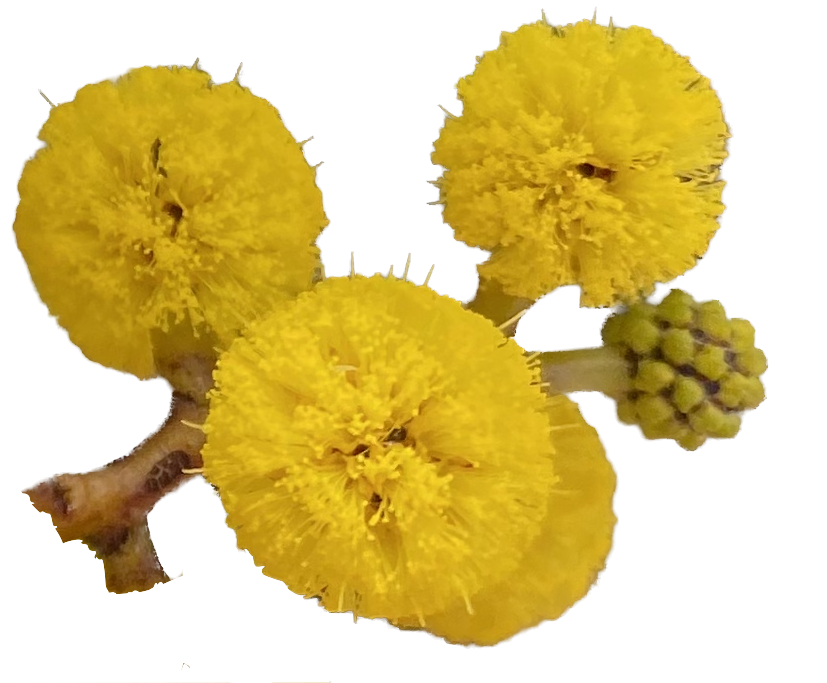
\includegraphics[width=1.5cm]{images/mulga-flowers2.png} % Adjust the image size as needed
    \end{minipage}%
    \hfill % Horizontal space between image and text
    \begin{minipage}[c]{0.8\linewidth} % Adjust width as needed for the text
      \bigskip%
      \textsf{#1}%
      \bigskip%
    \end{minipage}%
    \hspace*{3mm}%
  \end{minipage}%
}%
}
\usepackage{booktabs}
\usepackage{caption}
\usepackage{longtable}
\usepackage{amsmath}
\usepackage{blkarray}
\usepackage[most]{tcolorbox}
\usepackage{xcolor}
\definecolor{info}{HTML}{CBC988}
\definecolor{infostripe}{HTML}{EAC024}
\definecolor{insight}{HTML}{E87C00}
\definecolor{grey}{RGB}{192, 192, 192}
\usepackage{imakeidx}
\makeindex
\makeatletter
\makeatother
\makeatletter
\@ifpackageloaded{bookmark}{}{\usepackage{bookmark}}
\makeatother
\makeatletter
\@ifpackageloaded{caption}{}{\usepackage{caption}}
\AtBeginDocument{%
\ifdefined\contentsname
  \renewcommand*\contentsname{Table of contents}
\else
  \newcommand\contentsname{Table of contents}
\fi
\ifdefined\listfigurename
  \renewcommand*\listfigurename{List of Figures}
\else
  \newcommand\listfigurename{List of Figures}
\fi
\ifdefined\listtablename
  \renewcommand*\listtablename{List of Tables}
\else
  \newcommand\listtablename{List of Tables}
\fi
\ifdefined\figurename
  \renewcommand*\figurename{Figure}
\else
  \newcommand\figurename{Figure}
\fi
\ifdefined\tablename
  \renewcommand*\tablename{Table}
\else
  \newcommand\tablename{Table}
\fi
}
\@ifpackageloaded{float}{}{\usepackage{float}}
\floatstyle{ruled}
\@ifundefined{c@chapter}{\newfloat{codelisting}{h}{lop}}{\newfloat{codelisting}{h}{lop}[chapter]}
\floatname{codelisting}{Listing}
\newcommand*\listoflistings{\listof{codelisting}{List of Listings}}
\makeatother
\makeatletter
\@ifpackageloaded{caption}{}{\usepackage{caption}}
\@ifpackageloaded{subcaption}{}{\usepackage{subcaption}}
\makeatother
\makeatletter
\@ifpackageloaded{tcolorbox}{}{\usepackage[skins,breakable]{tcolorbox}}
\makeatother
\makeatletter
\@ifundefined{shadecolor}{\definecolor{shadecolor}{rgb}{.97, .97, .97}}
\makeatother
\makeatletter
\makeatother
\makeatletter
\makeatother
\ifLuaTeX
  \usepackage{selnolig}  % disable illegal ligatures
\fi
\IfFileExists{bookmark.sty}{\usepackage{bookmark}}{\usepackage{hyperref}}
\IfFileExists{xurl.sty}{\usepackage{xurl}}{} % add URL line breaks if available
\urlstyle{same} % disable monospaced font for URLs
\hypersetup{
  pdftitle={Interactively exploring high-dimensional data and models in R},
  pdfauthor={Dianne Cook and Ursula Laa},
  colorlinks=true,
  linkcolor={blue},
  filecolor={Maroon},
  citecolor={Blue},
  urlcolor={Blue},
  pdfcreator={LaTeX via pandoc}}

\title{Interactively exploring high-dimensional data and models in R}
\author{Dianne Cook and Ursula Laa}
\date{2024-01-26}

\begin{document}
\maketitle
\ifdefined\Shaded\renewenvironment{Shaded}{\begin{tcolorbox}[enhanced, boxrule=0pt, frame hidden, borderline west={3pt}{0pt}{shadecolor}, breakable, interior hidden, sharp corners]}{\end{tcolorbox}}\fi

\renewcommand*\contentsname{Table of contents}
{
\hypersetup{linkcolor=}
\setcounter{tocdepth}{2}
\tableofcontents
}
\bookmarksetup{startatroot}

\hypertarget{preface}{%
\chapter*{Preface}\label{preface}}
\addcontentsline{toc}{chapter}{Preface}

\markboth{Preface}{Preface}

It is important to visualise your data because you might discover things
that you could never have anticipated. Although there are many resources
available for data visualisation, there are few comprehensive resources
on high-dimensional data visualisation. High-dimensional (or
multivariate) data arises when many different things are measured for
each observation. While we can learn many things from plotting with 1D
and 2D or 3D methods there are likely more structures hidden in the
higher dimensions. This book provides guidance on visualising
high-dimensional data and models using linear projections, with R.

High-dimensional data spaces are fascinating places. You may think that
there's a lot of ways to plot one or two variables, and a lot of types
of patterns that can be found. You might use a density plot and see
skewness or a dot plot to find outliers. A scatterplot of two variables
might reveal a non-linear relationship or a barrier beyond which no
observations exist. We don't as yet have so many different choices of
plot types for high-dimensions, but these types of patterns are also
what we seek in scatterplots of high-dimensional data. The additional
dimensions can clarify these patterns, that clusters are likely to be
more distinct. Observations that did not appear to be very different can
be seen to be lonely anomalies in high-dimensions, that no other
observations have quite the same combination of values.

\hypertarget{whats-in-this-book}{%
\section*{What's in this book?}\label{whats-in-this-book}}
\addcontentsline{toc}{section}{What's in this book?}

\markright{What's in this book?}

The book is divided into these parts:

\begin{itemize}
\tightlist
\item
  \textbf{Introduction}: Here we introduce you to high-dimensional
  spaces, how they can be visualised, and notation that is useful for
  describing methods in later chapters.\\
\item
  \textbf{Dimension reduction}: This part covers linear and non-linear
  dimension reduction. It includes ways to help decide on the number of
  dimensions needed to summarise the high dimensional data, whether
  linear dimension reduction is appropriate, detecting problems that
  might affect the dimension reduction, and examining how well or badly
  a non-linear dimension reduction is representing the data.
\item
  \textbf{Cluster analysis}: This part described methods for finding
  groups in data. Although it includes an explanation of a purely
  graphical approach, it is mostly on using graphics in association with
  numerical clustering algorithms. There are explanations of assessing
  the suitability of different numerical techniques for extracting
  clusters, based on the data shapes, evaluating the clustering result,
  and showing the solutions in high dimensions.
\item
  \textbf{Classification}: This part describes methods for exploring
  known groups in the data. You'll learn how to check model assumptions,
  to help decide if a method is suited to the data, examine
  classification boundaries and explore where errors arise.
\item
  \textbf{Miscellaneous}: The material in this part focuses on examining
  data from different contexts. This includes multiple time series,
  longitudinal data. A key pre-processing step is to convert the data
  into Euclidean space.
\end{itemize}

In each of these parts an emphasis is also showing your model with your
data in the high dimensional space.

Our hopes are that you will come away with understanding the importance
of plotting your high dimensional data as a regular step in your
statistical or machine learning analyses. There are many examples of
what you might miss if you don't plot the data. Effective use of
graphics goes hand-in-hand with analytical techniques. With high
dimensions visualisation is a challenge but it is fascinating, and leads
to many surprising moments.

\hypertarget{audience}{%
\section*{Audience}\label{audience}}
\addcontentsline{toc}{section}{Audience}

\markright{Audience}

High-dimensional data arises in many fields such as biology, social
sciences, finance, and more. Anyone who is doing exploratory data
analysis and model fitting for more than two variables will benefit from
learning how to effectively visualise high-dimensions. This book will be
useful for students and teachers of multivariate data analysis and
machine learning, and researchers, data analysts, and industry
professionals who work in these areas.

\hypertarget{how-to-use-the-book}{%
\section*{How to use the book?}\label{how-to-use-the-book}}
\addcontentsline{toc}{section}{How to use the book?}

\markright{How to use the book?}

The book is written with explanations accompanied by examples with R
code. The chapters are organised by types of analysis and focus on how
to use the high-dimensional visualisation to complement the commonly
used analytical methods. The toolbox chapter in the Appendix provides an
overview of the primary high-dimensional visualisation methods discussed
in the book and how to get started.

\hypertarget{what-should-i-know-before-reading-this-book}{%
\section*{What should I know before reading this
book?}\label{what-should-i-know-before-reading-this-book}}
\addcontentsline{toc}{section}{What should I know before reading this
book?}

\markright{What should I know before reading this book?}

The examples assume that you already use R, and have a working knowledge
of base R and tidyverse way of thinking about data analysis. It also
assumes that you have some knowledge of statistical methods, and some
experience with machine learning methods.

If you feel like you need build up your skills in these areas in
preparation for working through this book, these are our recommended
resources:

\begin{itemize}
\tightlist
\item
  \href{https://r4ds.had.co.nz}{R for Data Science} by Wickham and
  Grolemund for learning about data wrangling and visualisation.
\item
  \href{https://openintro-ims.netlify.app}{Introduction to Modern
  Statistics} by Çetinkaya-Rundel and Hardin to learn about introductory
  statistics.
\item
  \href{https://bradleyboehmke.github.io/HOML/}{Hands-On Machine
  Learning with R} by Boehmke and Greenwell to learn about machine
  learning.
\end{itemize}

We will assume you know how to plot your data and models in 2D. Our
material starts from 2D and beyond.

\hypertarget{setting-up-your-workflow}{%
\section*{Setting up your workflow}\label{setting-up-your-workflow}}
\addcontentsline{toc}{section}{Setting up your workflow}

\markright{Setting up your workflow}

To get started set up your computer with the current versions of
\href{https://cran.r-project.org}{R} and ideally also with
\href{https://posit.co/download/rstudio-desktop/}{Rstudio Desktop}.

In addition, we have made an R package to share the data and functions
used in this book, called
\href{http://dicook.github.io/mulgar}{\texttt{mulgar}}.\footnote{Mulga
  is a type of Australian habitat composed of woodland or open forest
  dominated by the mulga tree. Massive clearing of mulga led to the vast
  wheat fields of Western Australia. Here \textbf{mulgar} is an acronym
  for \textbf{MUL}tivariate \textbf{G}raphical \textbf{A}nalysis with
  \textbf{R}.}\footnote{Photo of mulga tree taken by L. G. Cook.}

\begin{Shaded}
\begin{Highlighting}[]
\FunctionTok{install.packages}\NormalTok{(}\StringTok{"mulgar"}\NormalTok{, }\AttributeTok{dependencies=}\ConstantTok{TRUE}\NormalTok{)}
\CommentTok{\# or the development version}
\NormalTok{devtools}\SpecialCharTok{::}\FunctionTok{install\_github}\NormalTok{(}\StringTok{"dicook/mulgar"}\NormalTok{)}
\end{Highlighting}
\end{Shaded}

To get a copy of the code and data used and an RStudio project to get
started, you can download with this code:

\begin{Shaded}
\begin{Highlighting}[]
\NormalTok{book\_url }\OtherTok{\textless{}{-}} \StringTok{"https://dicook.github.io/mulgar\_book/code\_and\_data.zip"}
\NormalTok{usethis}\SpecialCharTok{::}\FunctionTok{use\_zip}\NormalTok{(}\AttributeTok{url=}\NormalTok{book\_url)}
\end{Highlighting}
\end{Shaded}

You will be able to click on the \texttt{mulgar\_book.Rproj} to get
started with the code.

\hypertarget{suggestion-feedback-or-error}{%
\section*{Suggestion, feedback or
error?}\label{suggestion-feedback-or-error}}
\addcontentsline{toc}{section}{Suggestion, feedback or error?}

\markright{Suggestion, feedback or error?}

We welcome suggestions, feedback or details of errors. You can report
them as an issue at the
\href{https://github.com/dicook/mulgar_book}{Github repo for this book}.

Please make a small \href{https://reprex.tidyverse.org}{reproducible
example} and report the error encountered. Reproducible examples have
these components:

\begin{itemize}
\tightlist
\item
  a small amount of data
\item
  small amount of code that generates the error
\item
  copy of the error message that was generated
\end{itemize}

\part{Introduction}

\hypertarget{intro}{%
\chapter{Picturing high dimensions}\label{intro}}

High-dimensional data means that we have a large number of numeric
features or variables, which can be considered as dimensions in a
mathematical space. The variables can be different types, such as
categorical or temporal, but the handling of these variables involves
different techniques. \index{dimensionality}
\index{variable}\index{feature} \index{projection}

\begin{figure*}

{\centering 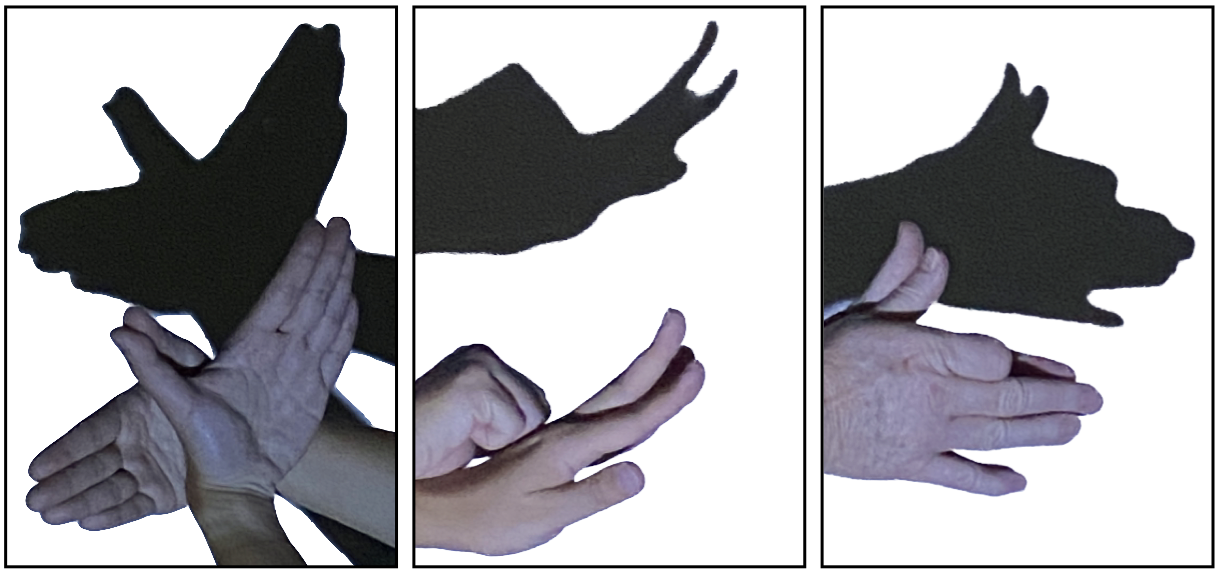
\includegraphics[width=4.6875in,height=\textheight]{images/shadow_puppets.png}

}

\end{figure*}

\hypertarget{getting-familiar-with-tours}{%
\section{Getting familiar with
tours}\label{getting-familiar-with-tours}}

\begin{figure*}

{\centering 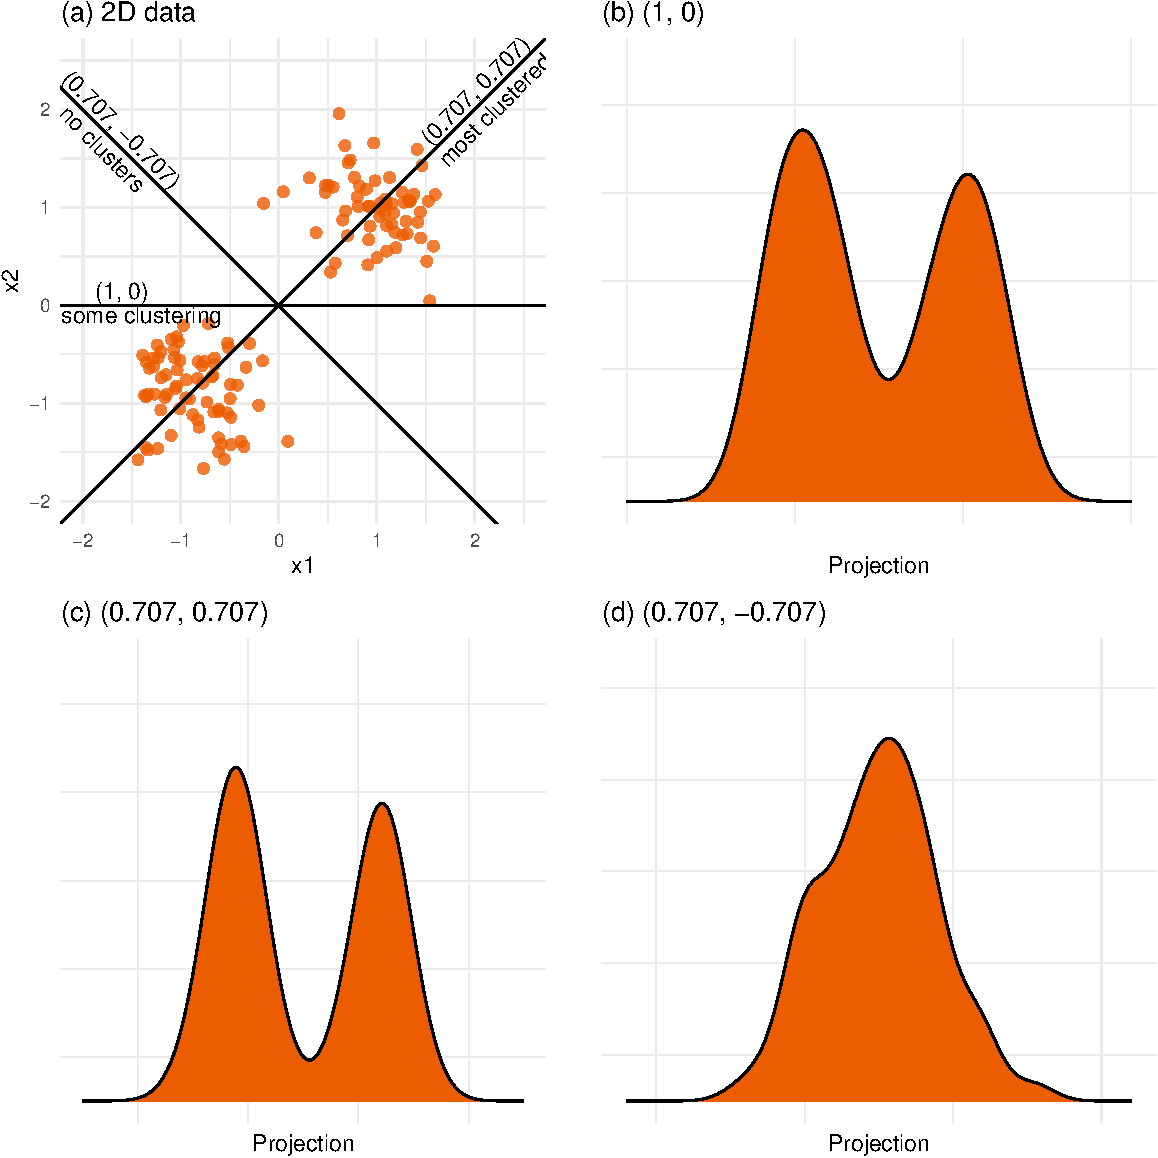
\includegraphics[width=1\textwidth,height=\textheight]{1-intro_files/figure-pdf/fig-explain-1D-pdf-1.pdf}

}

\caption{\label{fig-explain-1D-pdf}How a tour can be used to explore
high-dimensional data illustrated using (a) 2D data with two clusters
and (b,c,d) 1D projections from a tour shown as a density plot. Imagine
spinning a line around the centre of the data plot, with points
projected orthogonally onto the line. With this data, when the line is
at \texttt{x1=x2\ (0.707,\ 0.707)} or \texttt{(-0.707,\ -0.707)} the
clustering is the strongest. When it is at
\texttt{x1=-x2\ \ (0.707,\ -0.707)} there is no clustering.}

\end{figure*}

Figure~\ref{fig-explain-1D-pdf} illustrates a tour for 2D data and 1D
projections. The (grand) tour will generate all possible 1D projections
of the data, and display with a univariate plot like a histogram or
density plot. For this data, the \texttt{simple\_clusters} data,
depending on the projection, the distribution might be clustered into
two groups (bimodal), or there might be no clusters (unimodal). In this
example, all projections are generated by rotating a line around the
centre of the plot. Clustering can be seen in many of the projections,
with the strongest being when the contribution of both variables is
equal, and the projection is \texttt{(0.707,\ \ 0.707)} or
\texttt{(-0.707,\ -0.707)}. (If you are curious about the number
\texttt{0.707}, read the last section of this chapter.)

\index{projection!1D}

\begin{figure*}

{\centering 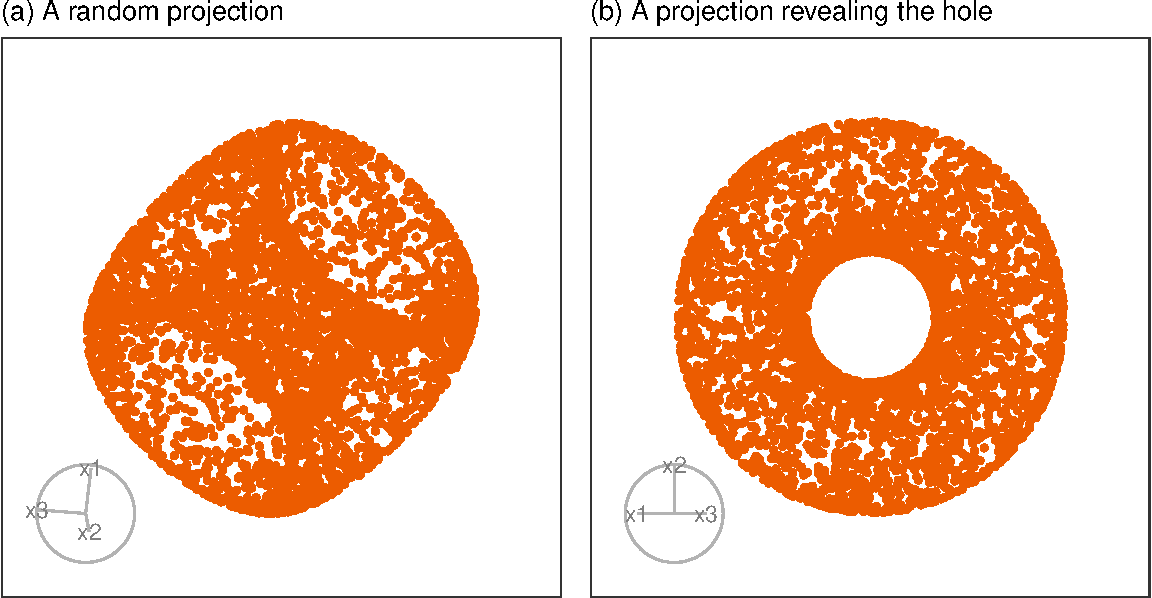
\includegraphics[width=1\textwidth,height=\textheight]{1-intro_files/figure-pdf/fig-explain-2D-pdf-1.pdf}

}

\caption{\label{fig-explain-2D-pdf}How a tour can be used to explore
high-dimensional data illustrated by showing a sequence of random 2D
projections of 3D data (a). The data has a donut shape with the hole
revealed in a single 2D projection (b). Data usually arrives with a
given number of observations, and when we plot it like this using a
scatterplot, it is like shadows of a transparent object.}

\end{figure*}

Figure~\ref{fig-explain-2D-pdf} illustrates a tour for 3D data using 2D
projections. The data are points on the surface of a donut shape. By
showing the projections using a scatterplot the donut looks transparent
and we can see through the data. The donut shape can be inferred from
watching many 2D projections but some are more revealing that others.
The projection shown in (b) is where the hole in the donut is clearly
visible. \index{projection!2D}

\hypertarget{whats-different-about-space-beyond-2d}{%
\section{What's different about space beyond
2D?}\label{whats-different-about-space-beyond-2d}}

The term ``high-dimensional'' in this book refers to the dimensionality
of the Euclidean space. Figure~\ref{fig-dimension-cubes} shows a way to
imagine this. It shows a sequence of cube wireframes, ranging from
one-dimensional (1D) through to five-dimensional (5D), where beyond 2D
is a linear projection of the cube. As the dimension increases, a new
orthogonal axis is added. For cubes, this is achieved by doubling the
cube: a 2D cube consists of two 1D cubes, a 3D cube consists of two 2D
cubes, and so forth. This is a great way to think about the space being
examined by the visual methods, and also all of the machine learning
methods mentioned, in this book.

\index{dimensionality}

\begin{figure}

{\centering 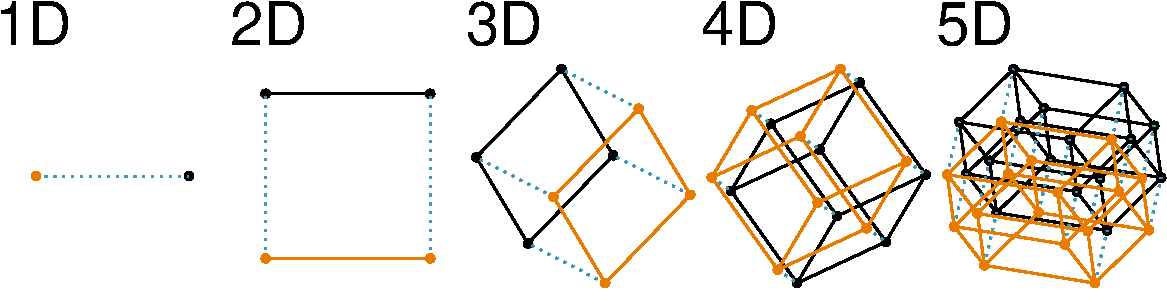
\includegraphics[width=0.8\textwidth,height=\textheight]{1-intro_files/figure-pdf/fig-dimension-cubes-1.pdf}

}

\caption{\label{fig-dimension-cubes}Space can be considered to be a
high-dimensional cube. Here we have pictured a sequence of increasing
dimension cubes, from 1D to 5D, as wireframes, it can be seen that as
the dimension increase by one, the cube doubles.}

\end{figure}

Interestingly, the struggle with imagining high-dimensions this way is
described in a novel published in 1884 (Abbott, 1884) \footnote{Thanks
  to Barret Schloerke for directing co-author Cook to this history when
  he was an undergraduate student and we were starting the
  \href{http://schloerke.com/geozoo/}{geozoo} project.}. Yes, more than
100 years ago! This is a story about characters living in a 2D world,
being visited by an alien 3D character. It also is a social satire,
serving the reader strong messages about gender inequity, although this
provides the means to explain more intricacies in perceiving dimensions.
There have been several movies made based on the book in recent decades
(e.g. Martin (1965), D. Johnson \& Travis (2007)). Although purchasing
the movies may be prohibitive, watching the trailers available for free
online is sufficient to gain enough geometric intuition on the nature of
understanding high-dimensional spaces while living in a low-dimensional
world.

When we look at high-dimensional spaces from a low-dimensional space, we
meet the ``curse of dimensionality'', a term introduced by Bellman
(1961) to express the difficulty of doing optimization in high
dimensions because of the exponential growth in space as dimension
increases. A way to imagine this is look at the cubes in
Figure~\ref{fig-dimension-cubes}: As you go from 1D to 2D, 2D to 3D, the
space expands a lot, and imagine how vast space might get as more
dimensions are added\footnote{``Space is big. Really big. You might
  think it's a long way to the pharmacy, but that's peanuts to space.''
  from Douglas Adams'
  \href{https://en.wikipedia.org/wiki/The_Hitchhiker\%27s_Guide_to_the_Galaxy\#Stage_shows}{Hitchhiker's
  Guide to the Galaxy} always springs to mind when thinking about high
  dimensions!}. The volume of the space grows exponentially with
dimension, which makes it infeasible to sample enough points -- any
sample will be less densely covering the space as dimension increases.
The effect is that most points will be far from the sample mean, on the
edge of the sample space.

\index{dimensionality!curse of}

For visualisation, the curse manifests in an opposite manner. Projecting
from high to low dimensions creates a crowding or piling of points near
the center of the distribution. This was noted by Diaconis \& Freedman
(1984a). Figure~\ref{fig-density} illustrates this phenomenon. As
dimension increases, the points crowd the centre, even with as few as
ten dimensions. This is something that we may need to correct for when
exploring high dimensions with low-dimensional projections.

\index{dimensionality!crowding}

\begin{figure}

{\centering 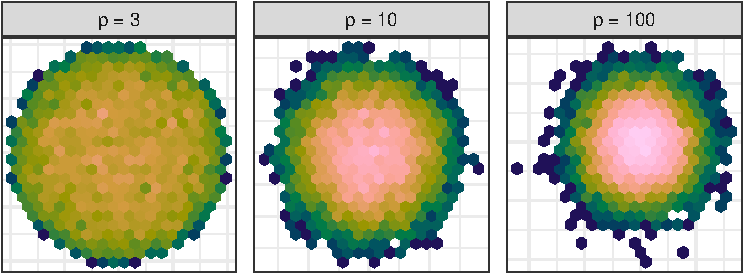
\includegraphics[width=0.95\textwidth,height=\textheight]{1-intro_files/figure-pdf/fig-density-1.pdf}

}

\caption{\label{fig-density}Illustration of data crowding in the
low-dimensional projection as dimension increases, here from 3, 10, 100.
Colour shows the number of points in each hexagon bin (pink is large,
navy is small). As dimension increases the points concentrate near the
centre.}

\end{figure}

Figure~\ref{fig-tour-intro-pdf} shows 2D tours of two different 5D data
sets. One has clusters (a) and the other has two outliers and a plane
(b). Can you see these? One difference in the viewing of data with more
than three dimensions with 2D projections is that the points seem to
shrink towards the centre, and then expand out again. This the effect of
dimensionality, with different variance or spread in some directions.

\begin{figure}

\begin{minipage}[t]{0.50\linewidth}

{\centering 

\raisebox{-\height}{

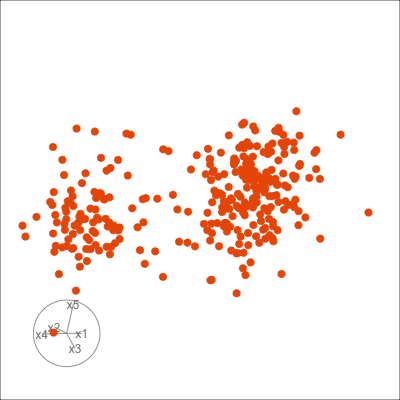
\includegraphics[width=2.08333in,height=\textheight]{images/clusters-intro.png}

}

}

\subcaption{\label{fig-tour-clusters}Clusters}
\end{minipage}%
%
\begin{minipage}[t]{0.50\linewidth}

{\centering 

\raisebox{-\height}{

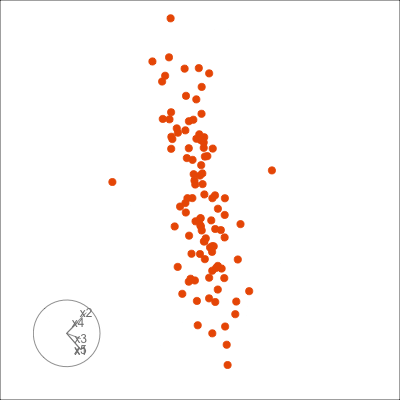
\includegraphics[width=2.08333in,height=\textheight]{images/outlier-intro.png}

}

}

\subcaption{\label{fig-tour-clusters}Outliers}
\end{minipage}%

\caption{\label{fig-tour-intro-pdf}Frames from 2D tours on two 5D
datasets, with clusters of points in (a) and two outliers with a plane
in (b). This figure is best viewed in the HTML version of the book.}

\end{figure}

\hypertarget{what-can-you-learn}{%
\section{What can you learn?}\label{what-can-you-learn}}

There are two ways of detecting structure in tours:

\begin{itemize}
\tightlist
\item
  patterns in a single low-dimensional projection
\item
  movement patterns
\end{itemize}

with the latter being especially useful when displaying the projected
data as a scatterplot. Figure~\ref{fig-example-structure} shows examples
of patterns we typically look for when making a scatterplot of data.
These include clustering, linear and non-linear association, outliers,
barriers where there is a sharp edge beyond which no observations are
seen. Not shown, but it also might be possible to observe multiple
modes, or density of observations, L-shapes, discreteness or uneven
spread of points. The tour is especially useful if these patterns are
only visible in combinations of variables.

\begin{figure}

{\centering 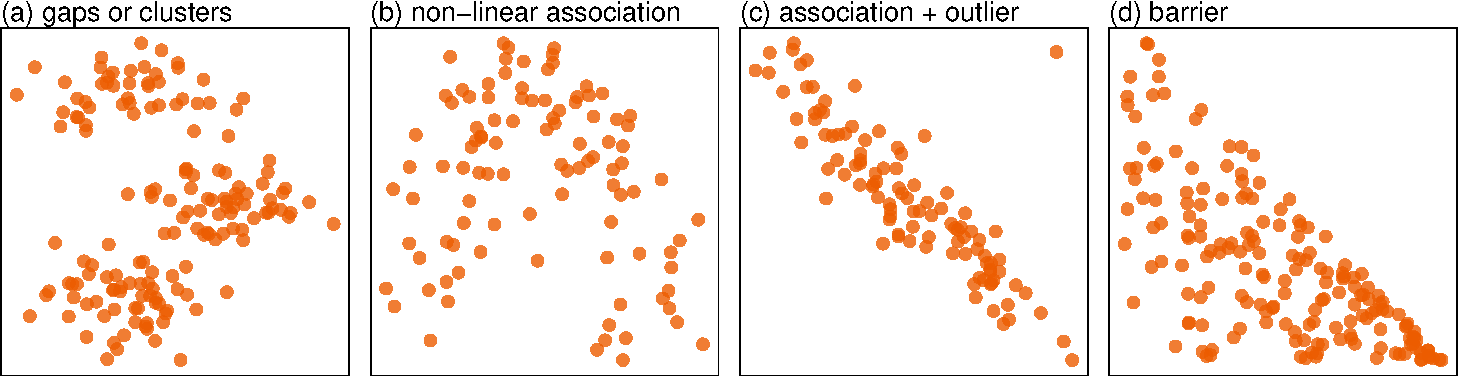
\includegraphics[width=1\textwidth,height=\textheight]{1-intro_files/figure-pdf/fig-example-structure-1.pdf}

}

\caption{\label{fig-example-structure}Example structures that might be
visible in a 2D projection that imply presence of structure in high
dimensions. These include clusters, linear and non-linear association,
outliers and barriers.}

\end{figure}

Figure~\ref{fig-trails} illustrates how movement patterns of points when
using scatterplots to display 2D projections indicate clustering (a, b)
and outliers (c, d).

\begin{figure}

\begin{minipage}[t]{0.50\linewidth}

{\centering 

\raisebox{-\height}{

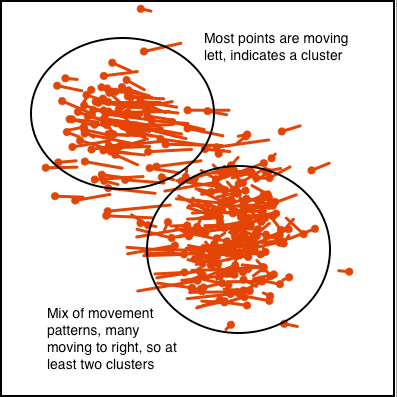
\includegraphics{images/trails-clusters.png}

}

}

\subcaption{\label{fig-clusters-trails-static}Clustering}
\end{minipage}%
%
\begin{minipage}[t]{0.50\linewidth}

{\centering 

\raisebox{-\height}{

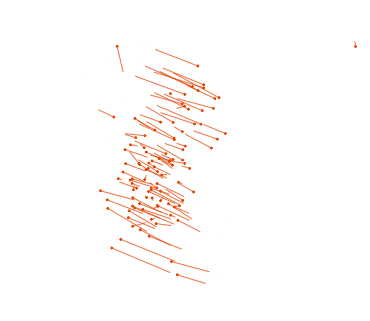
\includegraphics{images/trails-outlier.png}

}

}

\subcaption{\label{fig-outlier-trails-static}Outliers}
\end{minipage}%

\caption{\label{fig-trails}The movement of points give further clues
about the structure of the data in high-dimensions. In the data with
clustering, often we can see a group of points moving differently from
the others. Because there are three clusters, you should see three
distinct movement patterns. It is similar with outliers, except these
may be individual points moving alone, and different from all others.
This can be seen in the static plot, one point (top left) has a movement
pattern upwards whereas most of the other observations near it are
moving down towards the right.}

\end{figure}

This type of visualisation is useful for many activities in dealing with
high-dimensional data, including:

\begin{itemize}
\tightlist
\item
  exploring high-dimensional data.
\item
  detecting if the data lives in a lower dimensional space than the
  number of variables.
\item
  checking assumptions required for multivariate models to be
  applicable.
\item
  check for potential problems in modeling such as multicollinearity
  among predictors.
\item
  checking assumptions required for probabilties calculated for
  statistical hypothesis testing to be valid.
\item
  diagnosing the fit of multivariate models.
\end{itemize}

\infobox{With a tour we slowly rotate the viewing direction, this allows us to see many individual projections and to track movement patterns. Look for interesting structures such as clusters or outlying points.}

\hypertarget{a-little-history}{%
\section{A little history}\label{a-little-history}}

Viewing high-dimensional data based on low-dimensional projections can
probably be traced back to the early work on principal component
analysis by Pearson (1901) and Hotelling (1933), which was extended to
known classes as part of discriminant analysis by Fisher (1936a).

With computer graphics, the capability of animating plots to show more
than a single best projection became possible. The video library (ASA
Statistical Graphics Section, 2023) is the best place to experience the
earliest work. Kruskal's 1962 animation of multidimensional scaling
showed the process of finding a good 2D representation of high
dimensional data, although the views are not projections. Chang's 1970
video shows her rotating a high dimensional point cloud along coordinate
axes to find a special projection where all the numbers align. The
classic video that must be watched is PRIM9 (Fisherkeller et al., 1973)
where a variety of interactive and dynamic tools are used together to
explore high dimensional physics data, documented in Fisherkeller et al.
(1974).

The methods in this book primarily emerge from Asimov (1985)'s grand
tour method. The algorithm provided the first smooth and continuous
sequence of low dimensional projections, and guaranteed that all
possible low dimensional projections were likely to be shown. The
algorithm was refined in Buja \& Asimov (1986) (and documented in detail
in Buja et al. (2005)) to make it \emph{efficiently} show all possible
projections. Since then there have been numerous varieties of tour
algorithms developed to focus on specific tasks in exploring high
dimensional data, and these are documented in S. Lee et al. (2022).

This book is an evolution from Cook \& Swayne (2007). One of the
difficulties in working on interactive and dynamic graphics research has
been the rapid change in technology. Programming languages have changed
a little (fortran to C to java to python) but graphics toolkits and
display devices have changed a lot! The tour software used in this book
evolved from XGobi, which was written in C and used the X Window System,
which was then rewritten in GGobi using gtk. The video library has
engaging videos of these software systems There have been several other
short-lived implementations, including orca (Sutherland et al., 2000a),
written in java, and cranvas (Xie et al., 2014), written in R with a
back-end provided by wrapper functions to qt libraries.

Although attempts were made with these ancestor systems to connect the
data plots to a statistical analysis system, these were always limited.
With the emergence of R, having graphics in the data analysis workflow
has been much easier, albeit at the cost of the interactivity with
graphics that matches the old systems. We are mostly using the R
package, \texttt{tourr} (Wickham et al., 2011a) for examples in this
book. It provides the machinery for running a tour, and has the
flexibility that it can be ported, modified, and used as a regular
element of data analysis.

\hypertarget{exercises}{%
\section*{Exercises}\label{exercises}}
\addcontentsline{toc}{section}{Exercises}

\markright{Exercises}

\begin{enumerate}
\def\labelenumi{\arabic{enumi}.}
\tightlist
\item
  Randomly generate data points that are uniformly distributed in a
  hyper-cube of 3, 5 and 10 dimensions, with 500 points in each sample,
  using the \texttt{cube.solid.random} function of the \texttt{geozoo}
  package. What differences do we expect to see? Now visualise each set
  in a grand tour and describe how they differ, and whether this matched
  your expectations?
\item
  Use the \texttt{geozoo} package to generate samples from different
  shapes and use them to get a better understanding of how shapes appear
  in a grand tour. You can start with exploring the conic spiral in 3D,
  a torus in 4D and points along the wire frame of a cube in 5D.
\item
  For each of the challenge data sets, \texttt{c1}, \ldots, \texttt{c7}
  from the \texttt{mulgar} package, use the grand tour to view and try
  to identify structure (outliers, clusters, non-linear relationships).
\end{enumerate}

\hypertarget{notation-conventions-and-r-objects}{%
\chapter{Notation conventions and R
objects}\label{notation-conventions-and-r-objects}}

The data can be considered to be a matrix of numbers with the columns
corresponding to variables, and the rows correspond to observations. It
can be helpful to write this in mathematical notation, like:

\begin{eqnarray*}
X_{n\times p} =
[X_1~X_2~\dots~X_p]_{n\times p} = \left[ \begin{array}{cccc}
X_{11} & X_{12} & \dots & X_{1p} \\
X_{21} & X_{22} & \dots & X_{2p}\\
\vdots & \vdots &  & \vdots \\
X_{n1} & X_{n2} & \dots & X_{np} \end{array} \right]_{n\times p}
\end{eqnarray*}

where \(X\) indicates the the \(n\times p\) data matrix, \(X_j\)
indicates variable \(j, j=1, \dots, p\) and \(X_{ij}\) indicates the
value \(j^{th}\) variable of the \(i^{th}\) observation. (It can be
confusing to distinguish whether one is referring to the observation or
a variable, because \(X_i\) is used to indicate observation also. When
this is done it is usually accompanied by qualifying words such as
\textbf{observation} \(X_3\), or \textbf{variable} \(X_3\).)

Having notation is helpful for concise explanations of different
methods, to explain how data is scaled, processed and projected for
various tasks, and how different quantities are calculated from the
data.

When there is a response variable(s), it is common to consider \(X\) to
be the predictors, and use \(Y\) to indicate the response variable(s).
\(Y\) could be a matrix, also, and would be \(n\times q\), where
commonly \(q=1\). \(Y\) could be numeric or categorical, and this would
change how it is handled with visualisation.

To make a low-dimensional projection (shadow) of the data, we need a
projection matrix:

\begin{eqnarray*}
A_{p\times d} = \left[ \begin{array}{cccc}
A_{11} & A_{12} & \dots & A_{1d} \\
A_{21} & A_{22} & \dots & A_{2d}\\
\vdots & \vdots &  & \vdots \\
A_{p1} & A_{p2} & \dots & A_{pd} \end{array} \right]_{p\times d}
\end{eqnarray*}

\(A\) should be an orthonormal matrix, which means that the
\(\sum_{j=1}^p A_{jk}^2=1, k=1, \dots, d\) (columns represent vectors of
length 1) and \(\sum_{j=1}^p A_{jk}A_{jl}=0, k,l=1, \dots, d; k\neq l\)
(columns represent vectors that are orthogonal to each other). In matrix
notation, this can be written as \(A^{\top}A = I_d\).

Then the projected data is written as:

\begin{eqnarray*}
Y_{n\times d} = XA = \left[ \begin{array}{cccc}
y_{11} & y_{12} & \dots & y_{1d} \\
y_{21} & y_{22} & \dots & y_{2d}\\
\vdots & \vdots &  & \vdots \\
y_{n1} & y_{n2} & \dots & y_{nd} \end{array} \right]_{n\times d}
\end{eqnarray*}

where \(y_{ij} = \sum_{k=1}^p X_{ik}A_{kj}\). Note that we are using
\(Y\) as the projected data here, as well as it possibly being used for
a response variable. Where necessary, this will be clarified with words
in the text, when notation is used in explanations later.

When using R, if we only have the data corresponding to \(X\) it makes
sense to use a \texttt{matrix} object. However, if the response variable
is included and it is categorical, then we might use a
\texttt{data.frame} or a \texttt{tibble} which can accommodate
non-numerical values. Then to work with the data, we can use the base R
methods:

\begin{Shaded}
\begin{Highlighting}[]
\NormalTok{X }\OtherTok{\textless{}{-}} \FunctionTok{matrix}\NormalTok{(}\FunctionTok{c}\NormalTok{(}\FloatTok{1.1}\NormalTok{, }\FloatTok{1.3}\NormalTok{, }\FloatTok{1.4}\NormalTok{, }\FloatTok{1.2}\NormalTok{, }
              \FloatTok{2.7}\NormalTok{, }\FloatTok{2.6}\NormalTok{, }\FloatTok{2.4}\NormalTok{, }\FloatTok{2.5}\NormalTok{, }
              \FloatTok{3.5}\NormalTok{, }\FloatTok{3.4}\NormalTok{, }\FloatTok{3.2}\NormalTok{, }\FloatTok{3.6}\NormalTok{), }
            \AttributeTok{ncol=}\DecValTok{4}\NormalTok{, }\AttributeTok{byrow=}\ConstantTok{TRUE}\NormalTok{)}
\NormalTok{X}
\end{Highlighting}
\end{Shaded}

\begin{verbatim}
     [,1] [,2] [,3] [,4]
[1,]  1.1  1.3  1.4  1.2
[2,]  2.7  2.6  2.4  2.5
[3,]  3.5  3.4  3.2  3.6
\end{verbatim}

which is a data matrix with \(n=3, p=4\) and to extract a column
(variable):

\begin{Shaded}
\begin{Highlighting}[]
\NormalTok{X[,}\DecValTok{2}\NormalTok{]}
\end{Highlighting}
\end{Shaded}

\begin{verbatim}
[1] 1.3 2.6 3.4
\end{verbatim}

or a row (observation):

\begin{Shaded}
\begin{Highlighting}[]
\NormalTok{X[}\DecValTok{2}\NormalTok{,]}
\end{Highlighting}
\end{Shaded}

\begin{verbatim}
[1] 2.7 2.6 2.4 2.5
\end{verbatim}

or an individual cell (value):

\begin{Shaded}
\begin{Highlighting}[]
\NormalTok{X[}\DecValTok{3}\NormalTok{,}\DecValTok{2}\NormalTok{]}
\end{Highlighting}
\end{Shaded}

\begin{verbatim}
[1] 3.4
\end{verbatim}

To make a projection we need an orthonormal matrix:

\begin{Shaded}
\begin{Highlighting}[]
\NormalTok{A }\OtherTok{\textless{}{-}} \FunctionTok{matrix}\NormalTok{(}\FunctionTok{c}\NormalTok{(}\FloatTok{0.707}\NormalTok{,}\FloatTok{0.707}\NormalTok{,}\DecValTok{0}\NormalTok{,}\DecValTok{0}\NormalTok{,}\DecValTok{0}\NormalTok{,}\DecValTok{0}\NormalTok{,}\FloatTok{0.707}\NormalTok{,}\FloatTok{0.707}\NormalTok{), }\AttributeTok{ncol=}\DecValTok{2}\NormalTok{, }\AttributeTok{byrow=}\ConstantTok{FALSE}\NormalTok{)}
\NormalTok{A}
\end{Highlighting}
\end{Shaded}

\begin{verbatim}
      [,1]  [,2]
[1,] 0.707 0.000
[2,] 0.707 0.000
[3,] 0.000 0.707
[4,] 0.000 0.707
\end{verbatim}

You can check that it is orthonormal by

\begin{Shaded}
\begin{Highlighting}[]
\FunctionTok{sum}\NormalTok{(A[,}\DecValTok{1}\NormalTok{]}\SpecialCharTok{\^{}}\DecValTok{2}\NormalTok{)}
\end{Highlighting}
\end{Shaded}

\begin{verbatim}
[1] 0.999698
\end{verbatim}

\begin{Shaded}
\begin{Highlighting}[]
\FunctionTok{sum}\NormalTok{(A[,}\DecValTok{1}\NormalTok{]}\SpecialCharTok{*}\NormalTok{A[,}\DecValTok{2}\NormalTok{])}
\end{Highlighting}
\end{Shaded}

\begin{verbatim}
[1] 0
\end{verbatim}

and make a projection using matrix multiplication:

\begin{Shaded}
\begin{Highlighting}[]
\NormalTok{X }\SpecialCharTok{\%*\%}\NormalTok{ A}
\end{Highlighting}
\end{Shaded}

\begin{verbatim}
       [,1]   [,2]
[1,] 1.6968 1.8382
[2,] 3.7471 3.4643
[3,] 4.8783 4.8076
\end{verbatim}

The seemingly magical number \texttt{0.707} used above and to create the
projection in Figure~\ref{fig-explain-1D-pdf} arises from normalising a
vector with equal contributions from each variable, \texttt{(1,\ 1)}.
Dividing by \texttt{sqrt(2)} gives \texttt{(0.707,\ 0.707)}.

The notation convention used throughout the book is:

\texttt{n\ =} number of observations \texttt{p\ =} number of variables,
dimension of data \texttt{d\ =} dimension of the projection
\texttt{g\ =} number of groups, in classification \texttt{X\ =} data
matrix

\hypertarget{exercises-1}{%
\section*{Exercises}\label{exercises-1}}
\addcontentsline{toc}{section}{Exercises}

\markright{Exercises}

\begin{enumerate}
\def\labelenumi{\arabic{enumi}.}
\tightlist
\item
  Generate a matrix \(A\) with \(p=5\) (rows) and \(d=2\) (columns),
  where each value is randomly drawn from a standard normal
  distribution. Extract the element at row 3 and column 1.
\item
  We will interpret \(A\) as a projection matrix and therefore it needs
  to be orthonormalised. Use the function \texttt{tourr::orthonormalise}
  to do this, and explicitly check that each column is normalised and
  that the two columns are orthogonal now. Which dimensions contribute
  most to the projection for your \(A\)?
\item
  Use matrix multiplication to calculate the projection of the
  \texttt{mulgar::clusters} data onto the 2D plane defined by \(A\).
  Make a scatterplot of the projected data. Can you identify clustering
  in this view?
\end{enumerate}

\part{Dimension reduction}

\hypertarget{sec-dimension-overview}{%
\chapter{Overview}\label{sec-dimension-overview}}

This chapter will focus on methods for reducing dimension, and how the
tour can be used to assist with the common methods such as principal
component analysis (PCA), multidimensional scaling (MDS), t-stochastic
neighbour embedding (t-SNE), and factor analysis.

Dimension is perceived in a tour using the spread of points. When the
points are spread far apart, then the data is filling the space.
Conversely when the points ``collapse'' into a sub-region then the data
is only partially filling the space, and some dimension reduction to
reduce to this smaller dimensional space may be worthwhile.

\infobox{When points do not fill the plotting canvas fully, it means that it lives in a lower dimension. This low-dimensional space might be linear or non-linear, with the latter being much harder to define and capture.}

Let's start with some 2D examples. You need at least two variables to be
able to talk about association between variables. Figure~\ref{fig-2D}
shows three plots of two variables. Plot (a) shows two variables that
are strongly linearly associated\footnote{It is generally better to use
  \emph{associated} than \emph{correlated}. Correlation is a statistical
  quantity, measuring linear association. The term \emph{associated} can
  be prefaced with the type of association, such as \emph{linear} or
  \emph{non-linear}.}, because when \texttt{x1} is low, \texttt{x2} is
low also, and conversely when \texttt{x1} is high, \texttt{x2} is also
high. This can also be seen by the reducton in spread of points (or
``collapse'') in one direction making the data fill less than the full
square of the plot. \emph{So from this we can conclude that the data is
not fully 2D.} The second step is to infer which variables contribute to
this reduction in dimension. The axes for \texttt{x1} and \texttt{x2}
are drawn extending from \((0,0)\) and because they both extend out of
the cloud of points, in the direction away from the collapse of points
we can say that they are jointly responsible for the dimension
reduction.

Figure~\ref{fig-2D} (b) shows a pair of variables that are \textbf{not}
linearly associated. Variable \texttt{x1} is more varied than
\texttt{x3} but knowing the value on \texttt{x1} tells us nothing about
possible values on \texttt{x3}. Before running a tour all variables are
typically scaled to have equal spread. The purpose of the tour is to
capture association and relationships between the variables, so any
univariate differences should be removed ahead of time.
Figure~\ref{fig-2D} (c) shows what this would look like when \texttt{x3}
is scaled - the points are fully spread in the full square of the plot.

\begin{Shaded}
\begin{Highlighting}[]
\FunctionTok{library}\NormalTok{(tibble)}
\FunctionTok{set.seed}\NormalTok{(}\DecValTok{6045}\NormalTok{)}
\NormalTok{x1 }\OtherTok{\textless{}{-}} \FunctionTok{runif}\NormalTok{(}\DecValTok{123}\NormalTok{)}
\NormalTok{x2 }\OtherTok{\textless{}{-}}\NormalTok{ x1 }\SpecialCharTok{+} \FunctionTok{rnorm}\NormalTok{(}\DecValTok{123}\NormalTok{, }\AttributeTok{sd=}\FloatTok{0.1}\NormalTok{)}
\NormalTok{x3 }\OtherTok{\textless{}{-}} \FunctionTok{rnorm}\NormalTok{(}\DecValTok{123}\NormalTok{, }\AttributeTok{sd=}\FloatTok{0.2}\NormalTok{)}
\NormalTok{df }\OtherTok{\textless{}{-}} \FunctionTok{tibble}\NormalTok{(}\AttributeTok{x1 =}\NormalTok{ (x1}\SpecialCharTok{{-}}\FunctionTok{mean}\NormalTok{(x1))}\SpecialCharTok{/}\FunctionTok{sd}\NormalTok{(x1), }
             \AttributeTok{x2 =}\NormalTok{ (x2}\SpecialCharTok{{-}}\FunctionTok{mean}\NormalTok{(x2))}\SpecialCharTok{/}\FunctionTok{sd}\NormalTok{(x2),}
\NormalTok{             x3, }
             \AttributeTok{x3scaled =}\NormalTok{ (x3}\SpecialCharTok{{-}}\FunctionTok{mean}\NormalTok{(x3))}\SpecialCharTok{/}\FunctionTok{sd}\NormalTok{(x3))}
\end{Highlighting}
\end{Shaded}

\begin{figure}

{\centering 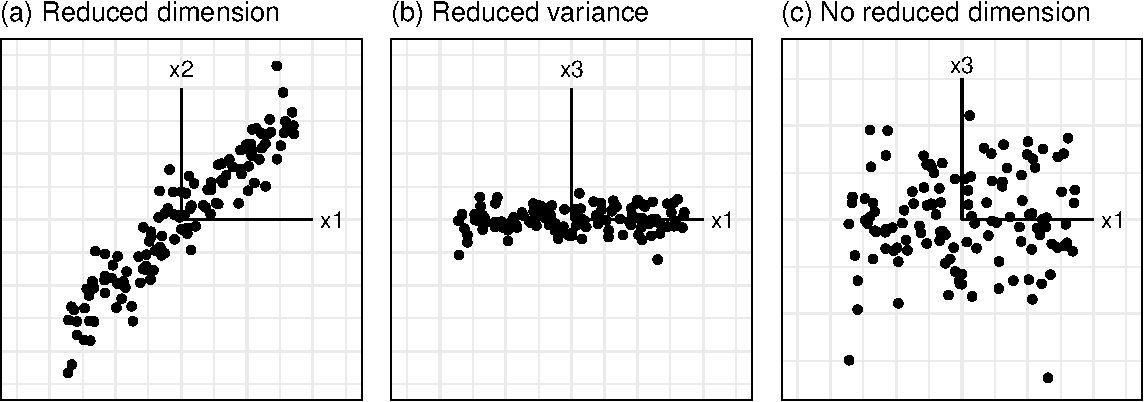
\includegraphics[width=1\textwidth,height=\textheight]{3-intro-dimred_files/figure-pdf/fig-2D-1.pdf}

}

\caption{\label{fig-2D}Explanation of how dimension reduction is
perceived in 2D, relative to variables: (a) Two variables with strong
linear association. Both variables contribute to the association, as
indicated by their axes extending out from the `collapsed' direction of
the points; (b) Two variables with no linear association. But x3 has
less variation, so points collapse in this direction; (c) The situation
in plot (b) does not arise in a tour because all variables are (usually)
scaled. When an axes extends out of a direction where the points are
collapsed, it means that this variable is partially responsible for the
reduced dimension.}

\end{figure}

Now let's think about what this looks like with five variables.
Figure~\ref{fig-dimension-pdf} shows a grand tour on five variables,
with (a) data that is primarily 2D, (b) data that is primarily 3D and
(c) fully 5D data. You can see that both (a) and (b) the spread of
points collapse in some projections, with it happening more in (a). In
(c) the data is always spread out in the square, although it does seem
to concentrate or pile in the centre. This piling is typical when
projecting from high dimensions to low dimensions. The sage tour (Laa et
al., 2020a) makes a correction for this.

\begin{Shaded}
\begin{Highlighting}[]
\FunctionTok{library}\NormalTok{(mulgar)}
\FunctionTok{data}\NormalTok{(plane)}
\FunctionTok{data}\NormalTok{(box)}
\FunctionTok{render\_gif}\NormalTok{(plane,}
           \FunctionTok{grand\_tour}\NormalTok{(), }
           \FunctionTok{display\_xy}\NormalTok{(),}
           \AttributeTok{gif\_file=}\StringTok{"gifs/plane.gif"}\NormalTok{,}
           \AttributeTok{frames=}\DecValTok{500}\NormalTok{,}
           \AttributeTok{width=}\DecValTok{200}\NormalTok{,}
           \AttributeTok{height=}\DecValTok{200}\NormalTok{)}
\FunctionTok{render\_gif}\NormalTok{(box,}
           \FunctionTok{grand\_tour}\NormalTok{(), }
           \FunctionTok{display\_xy}\NormalTok{(),}
           \AttributeTok{gif\_file=}\StringTok{"gifs/box.gif"}\NormalTok{,}
           \AttributeTok{frames=}\DecValTok{500}\NormalTok{,}
           \AttributeTok{width=}\DecValTok{200}\NormalTok{,}
           \AttributeTok{height=}\DecValTok{200}\NormalTok{)}
\CommentTok{\# Simulate full cube}
\FunctionTok{library}\NormalTok{(geozoo)}
\NormalTok{cube5d }\OtherTok{\textless{}{-}} \FunctionTok{data.frame}\NormalTok{(}\FunctionTok{cube.solid.random}\NormalTok{(}\AttributeTok{p=}\DecValTok{5}\NormalTok{, }\AttributeTok{n=}\DecValTok{300}\NormalTok{)}\SpecialCharTok{$}\NormalTok{points)}
\FunctionTok{colnames}\NormalTok{(cube5d) }\OtherTok{\textless{}{-}} \FunctionTok{paste0}\NormalTok{(}\StringTok{"x"}\NormalTok{, }\DecValTok{1}\SpecialCharTok{:}\DecValTok{5}\NormalTok{)}
\NormalTok{cube5d }\OtherTok{\textless{}{-}} \FunctionTok{data.frame}\NormalTok{(}\FunctionTok{apply}\NormalTok{(cube5d, }\DecValTok{2}\NormalTok{, }\ControlFlowTok{function}\NormalTok{(x) (x}\SpecialCharTok{{-}}\FunctionTok{mean}\NormalTok{(x))}\SpecialCharTok{/}\FunctionTok{sd}\NormalTok{(x)))}
\FunctionTok{render\_gif}\NormalTok{(cube5d,}
           \FunctionTok{grand\_tour}\NormalTok{(), }
           \FunctionTok{display\_xy}\NormalTok{(),}
           \AttributeTok{gif\_file=}\StringTok{"gifs/cube5d.gif"}\NormalTok{,}
           \AttributeTok{frames=}\DecValTok{500}\NormalTok{,}
           \AttributeTok{width=}\DecValTok{200}\NormalTok{,}
           \AttributeTok{height=}\DecValTok{200}\NormalTok{)}
\end{Highlighting}
\end{Shaded}

\begin{figure}

\begin{minipage}[t]{0.33\linewidth}

{\centering 

\raisebox{-\height}{

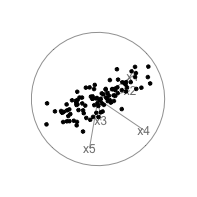
\includegraphics[width=1.66667in,height=\textheight]{images/plane.png}

}

}

\subcaption{\label{fig-plane}2D plane in 5D}
\end{minipage}%
%
\begin{minipage}[t]{0.33\linewidth}

{\centering 

\raisebox{-\height}{

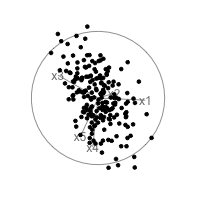
\includegraphics[width=1.66667in,height=\textheight]{images/box.png}

}

}

\subcaption{\label{fig-box}3D plane in 5D}
\end{minipage}%
%
\begin{minipage}[t]{0.33\linewidth}

{\centering 

\raisebox{-\height}{

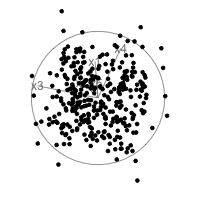
\includegraphics[width=1.66667in,height=\textheight]{images/cube5d.png}

}

}

\subcaption{\label{fig-cube5}5D plane in 5D}
\end{minipage}%

\caption{\label{fig-dimension-pdf}Single frames from different
dimensional planes - 2D, 3D, 5D - displayed in a grand tour projecting
into 2D. Notice that the 5D in 5D always fills out the box (although it
does concentrate some in the middle which is typical when projecting
from high to low dimensions). Also you can see that the 2D in 5D,
concentrates into a line more than the 3D in 5D. This suggests that it
is lower dimensional. (Animations can be viewed
\href{https://dicook.github.io/mulgar_book/3-intro-dimred.html}{here}.)}

\end{figure}

The next step is to determine which variables contribute. In the
examples just provided, all variables are linearly associated in the 2D
and 3D data. You can check this by making a scatterplot matrix,
Figure~\ref{fig-plane-scatmat}.

\begin{Shaded}
\begin{Highlighting}[]
\FunctionTok{library}\NormalTok{(GGally)}
\FunctionTok{library}\NormalTok{(mulgar)}
\FunctionTok{data}\NormalTok{(plane)}
\FunctionTok{ggscatmat}\NormalTok{(plane) }\SpecialCharTok{+}
  \FunctionTok{theme}\NormalTok{(}\AttributeTok{panel.background =} 
          \FunctionTok{element\_rect}\NormalTok{(}\AttributeTok{colour=}\StringTok{"black"}\NormalTok{, }\AttributeTok{fill=}\ConstantTok{NA}\NormalTok{),}
    \AttributeTok{axis.text =} \FunctionTok{element\_blank}\NormalTok{(),}
    \AttributeTok{axis.ticks =} \FunctionTok{element\_blank}\NormalTok{())}
\end{Highlighting}
\end{Shaded}

\begin{figure}[H]

{\centering 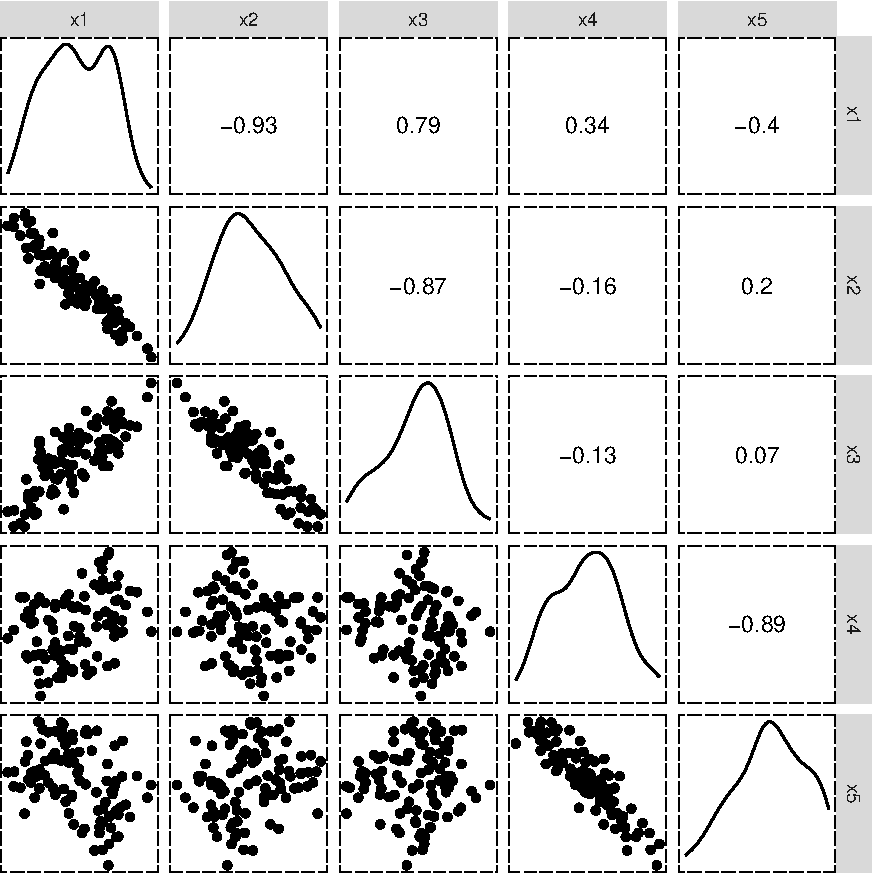
\includegraphics[width=0.8\textwidth,height=\textheight]{3-intro-dimred_files/figure-pdf/fig-plane-scatmat-1.pdf}

}

\caption{\label{fig-plane-scatmat}Scatterplot matrix of plane data. You
can see that x1-x3 are strongly linearly associated, and also x4 and x5.
When you watch the tour of this data, any time the data collapses into a
line you should see only (x1, x2, x3) or (x4, x5). When combinations of
x1 and x4 or x5 show, the data should be spread out.}

\end{figure}

To make an example where not all variables contribute, we have added two
additional variables to the \texttt{plane} data set, which are purely
noise.

\begin{Shaded}
\begin{Highlighting}[]
\CommentTok{\# Add two pure noise dimensions to the plane}
\NormalTok{plane\_noise }\OtherTok{\textless{}{-}}\NormalTok{ plane}
\NormalTok{plane\_noise}\SpecialCharTok{$}\NormalTok{x6 }\OtherTok{\textless{}{-}} \FunctionTok{rnorm}\NormalTok{(}\DecValTok{100}\NormalTok{)}
\NormalTok{plane\_noise}\SpecialCharTok{$}\NormalTok{x7 }\OtherTok{\textless{}{-}} \FunctionTok{rnorm}\NormalTok{(}\DecValTok{100}\NormalTok{)}
\NormalTok{plane\_noise }\OtherTok{\textless{}{-}} \FunctionTok{data.frame}\NormalTok{(}\FunctionTok{apply}\NormalTok{(plane\_noise, }\DecValTok{2}\NormalTok{, }
    \ControlFlowTok{function}\NormalTok{(x) (x}\SpecialCharTok{{-}}\FunctionTok{mean}\NormalTok{(x))}\SpecialCharTok{/}\FunctionTok{sd}\NormalTok{(x)))}
\FunctionTok{ggduo}\NormalTok{(plane\_noise, }\AttributeTok{columnsX =} \DecValTok{1}\SpecialCharTok{:}\DecValTok{5}\NormalTok{, }\AttributeTok{columnsY =} \DecValTok{6}\SpecialCharTok{:}\DecValTok{7}\NormalTok{, }
    \AttributeTok{types =} \FunctionTok{list}\NormalTok{(}\AttributeTok{continuous =} \StringTok{"points"}\NormalTok{)) }\SpecialCharTok{+}
  \FunctionTok{theme}\NormalTok{(}\AttributeTok{aspect.ratio=}\DecValTok{1}\NormalTok{,}
    \AttributeTok{panel.background =} 
          \FunctionTok{element\_rect}\NormalTok{(}\AttributeTok{colour=}\StringTok{"black"}\NormalTok{, }\AttributeTok{fill=}\ConstantTok{NA}\NormalTok{),}
    \AttributeTok{axis.text =} \FunctionTok{element\_blank}\NormalTok{(),}
    \AttributeTok{axis.ticks =} \FunctionTok{element\_blank}\NormalTok{())}
\end{Highlighting}
\end{Shaded}

\begin{figure}[H]

{\centering 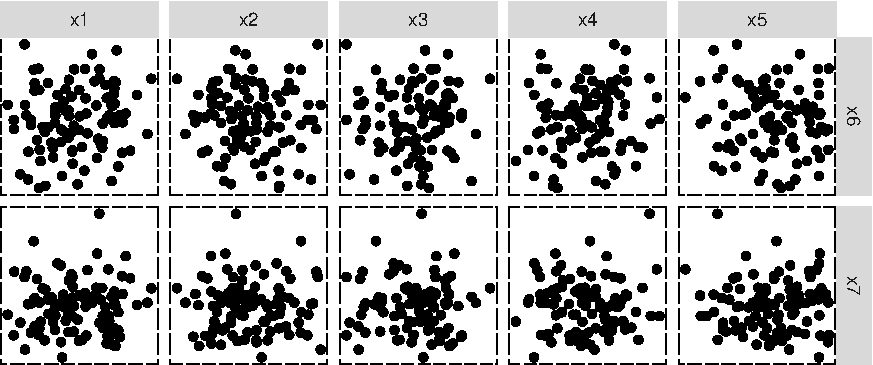
\includegraphics[width=0.8\textwidth,height=\textheight]{3-intro-dimred_files/figure-pdf/fig-plane-noise-scatter-1.pdf}

}

\caption{\label{fig-plane-noise-scatter}Scatterplots showing two
additional noise variables that are not associated with any of the first
five variables.}

\end{figure}

Now we have 2D structure in 7D, but only five of the variables
contribute to the 2D structure, that is, five of the variables are
linearly related with each other. The other two variables (x6, x7) are
not linearly related to any of the others.

The data is viewed with a grand tour in
Figure~\ref{fig-plane-noise-pdf}. We can still see the concentration of
points along a line in some dimensions, which tells us that the data is
not fully 7D. Then if you look closely at the variable axes you will see
that the collapsing to a line only occurs when any of x1-x5 contribute
strongly in the direction orthogonal to this. This does not happen when
x6 or x7 contribute strongly to a projection - the data is always
expanded to fill much of the space. That tells us that x6 and x7 don't
substantially contribute to the dimension reduction, that is, they are
not linearly related to the other variables.

\begin{Shaded}
\begin{Highlighting}[]
\FunctionTok{library}\NormalTok{(ggplot2)}
\FunctionTok{library}\NormalTok{(plotly)}
\FunctionTok{library}\NormalTok{(htmlwidgets)}

\FunctionTok{set.seed}\NormalTok{(}\DecValTok{78}\NormalTok{)}
\NormalTok{b }\OtherTok{\textless{}{-}} \FunctionTok{basis\_random}\NormalTok{(}\DecValTok{7}\NormalTok{, }\DecValTok{2}\NormalTok{)}
\NormalTok{pn\_t }\OtherTok{\textless{}{-}}\NormalTok{ tourr}\SpecialCharTok{::}\FunctionTok{save\_history}\NormalTok{(plane\_noise, }
                    \AttributeTok{tour\_path =} \FunctionTok{grand\_tour}\NormalTok{(),}
                    \AttributeTok{start =}\NormalTok{ b,}
                    \AttributeTok{max\_bases =} \DecValTok{8}\NormalTok{)}
\NormalTok{pn\_t }\OtherTok{\textless{}{-}} \FunctionTok{interpolate}\NormalTok{(pn\_t, }\FloatTok{0.1}\NormalTok{)}
\NormalTok{pn\_anim }\OtherTok{\textless{}{-}} \FunctionTok{render\_anim}\NormalTok{(plane\_noise,}
                         \AttributeTok{frames=}\NormalTok{pn\_t)}

\NormalTok{pn\_gp }\OtherTok{\textless{}{-}} \FunctionTok{ggplot}\NormalTok{() }\SpecialCharTok{+}
     \FunctionTok{geom\_path}\NormalTok{(}\AttributeTok{data=}\NormalTok{pn\_anim}\SpecialCharTok{$}\NormalTok{circle, }
               \FunctionTok{aes}\NormalTok{(}\AttributeTok{x=}\NormalTok{c1, }\AttributeTok{y=}\NormalTok{c2,}
                   \AttributeTok{frame=}\NormalTok{frame), }\AttributeTok{linewidth=}\FloatTok{0.1}\NormalTok{) }\SpecialCharTok{+}
     \FunctionTok{geom\_segment}\NormalTok{(}\AttributeTok{data=}\NormalTok{pn\_anim}\SpecialCharTok{$}\NormalTok{axes, }
                  \FunctionTok{aes}\NormalTok{(}\AttributeTok{x=}\NormalTok{x1, }\AttributeTok{y=}\NormalTok{y1, }
                      \AttributeTok{xend=}\NormalTok{x2, }\AttributeTok{yend=}\NormalTok{y2, }
                      \AttributeTok{frame=}\NormalTok{frame), }
                  \AttributeTok{linewidth=}\FloatTok{0.1}\NormalTok{) }\SpecialCharTok{+}
     \FunctionTok{geom\_text}\NormalTok{(}\AttributeTok{data=}\NormalTok{pn\_anim}\SpecialCharTok{$}\NormalTok{axes, }
               \FunctionTok{aes}\NormalTok{(}\AttributeTok{x=}\NormalTok{x2, }\AttributeTok{y=}\NormalTok{y2, }
                   \AttributeTok{frame=}\NormalTok{frame, }
                   \AttributeTok{label=}\NormalTok{axis\_labels), }
               \AttributeTok{size=}\DecValTok{5}\NormalTok{) }\SpecialCharTok{+}
     \FunctionTok{geom\_point}\NormalTok{(}\AttributeTok{data=}\NormalTok{pn\_anim}\SpecialCharTok{$}\NormalTok{frames, }
                \FunctionTok{aes}\NormalTok{(}\AttributeTok{x=}\NormalTok{P1, }\AttributeTok{y=}\NormalTok{P2, }
                    \AttributeTok{frame=}\NormalTok{frame), }
                \AttributeTok{alpha=}\FloatTok{0.8}\NormalTok{) }\SpecialCharTok{+}
     \FunctionTok{xlim}\NormalTok{(}\SpecialCharTok{{-}}\DecValTok{1}\NormalTok{,}\DecValTok{1}\NormalTok{) }\SpecialCharTok{+} \FunctionTok{ylim}\NormalTok{(}\SpecialCharTok{{-}}\DecValTok{1}\NormalTok{,}\DecValTok{1}\NormalTok{) }\SpecialCharTok{+}
     \FunctionTok{coord\_equal}\NormalTok{() }\SpecialCharTok{+}
     \FunctionTok{theme\_bw}\NormalTok{() }\SpecialCharTok{+}
     \FunctionTok{theme}\NormalTok{(}\AttributeTok{axis.text=}\FunctionTok{element\_blank}\NormalTok{(),}
         \AttributeTok{axis.title=}\FunctionTok{element\_blank}\NormalTok{(),}
         \AttributeTok{axis.ticks=}\FunctionTok{element\_blank}\NormalTok{(),}
         \AttributeTok{panel.grid=}\FunctionTok{element\_blank}\NormalTok{())}
\NormalTok{pn\_tour }\OtherTok{\textless{}{-}} \FunctionTok{ggplotly}\NormalTok{(pn\_gp,}
                        \AttributeTok{width=}\DecValTok{500}\NormalTok{,}
                        \AttributeTok{height=}\DecValTok{550}\NormalTok{) }\SpecialCharTok{\%\textgreater{}\%}
       \FunctionTok{animation\_button}\NormalTok{(}\AttributeTok{label=}\StringTok{"Go"}\NormalTok{) }\SpecialCharTok{\%\textgreater{}\%}
       \FunctionTok{animation\_slider}\NormalTok{(}\AttributeTok{len=}\FloatTok{0.8}\NormalTok{, }\AttributeTok{x=}\FloatTok{0.5}\NormalTok{,}
                        \AttributeTok{xanchor=}\StringTok{"center"}\NormalTok{) }\SpecialCharTok{\%\textgreater{}\%}
       \FunctionTok{animation\_opts}\NormalTok{(}\AttributeTok{easing=}\StringTok{"linear"}\NormalTok{, }
                      \AttributeTok{transition =} \DecValTok{0}\NormalTok{)}

\NormalTok{htmlwidgets}\SpecialCharTok{::}\FunctionTok{saveWidget}\NormalTok{(pn\_tour,}
          \AttributeTok{file=}\StringTok{"html/plane\_noise.html"}\NormalTok{,}
          \AttributeTok{selfcontained =} \ConstantTok{TRUE}\NormalTok{)}
\end{Highlighting}
\end{Shaded}

\begin{figure}

\begin{minipage}[t]{0.50\linewidth}

{\centering 

\raisebox{-\height}{

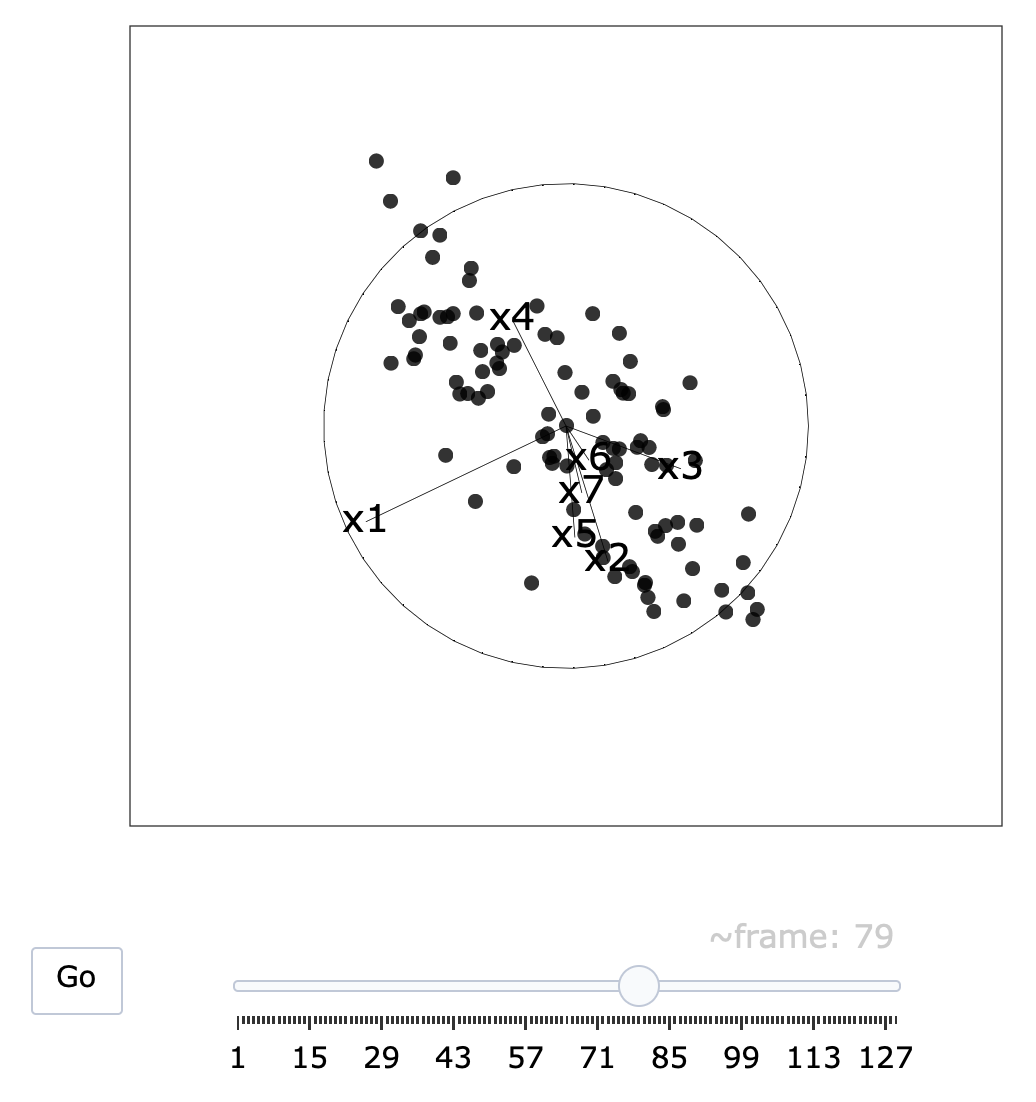
\includegraphics[width=2.08333in,height=\textheight]{images/plane_noise1.png}

}

}

\end{minipage}%
%
\begin{minipage}[t]{0.50\linewidth}

{\centering 

\raisebox{-\height}{

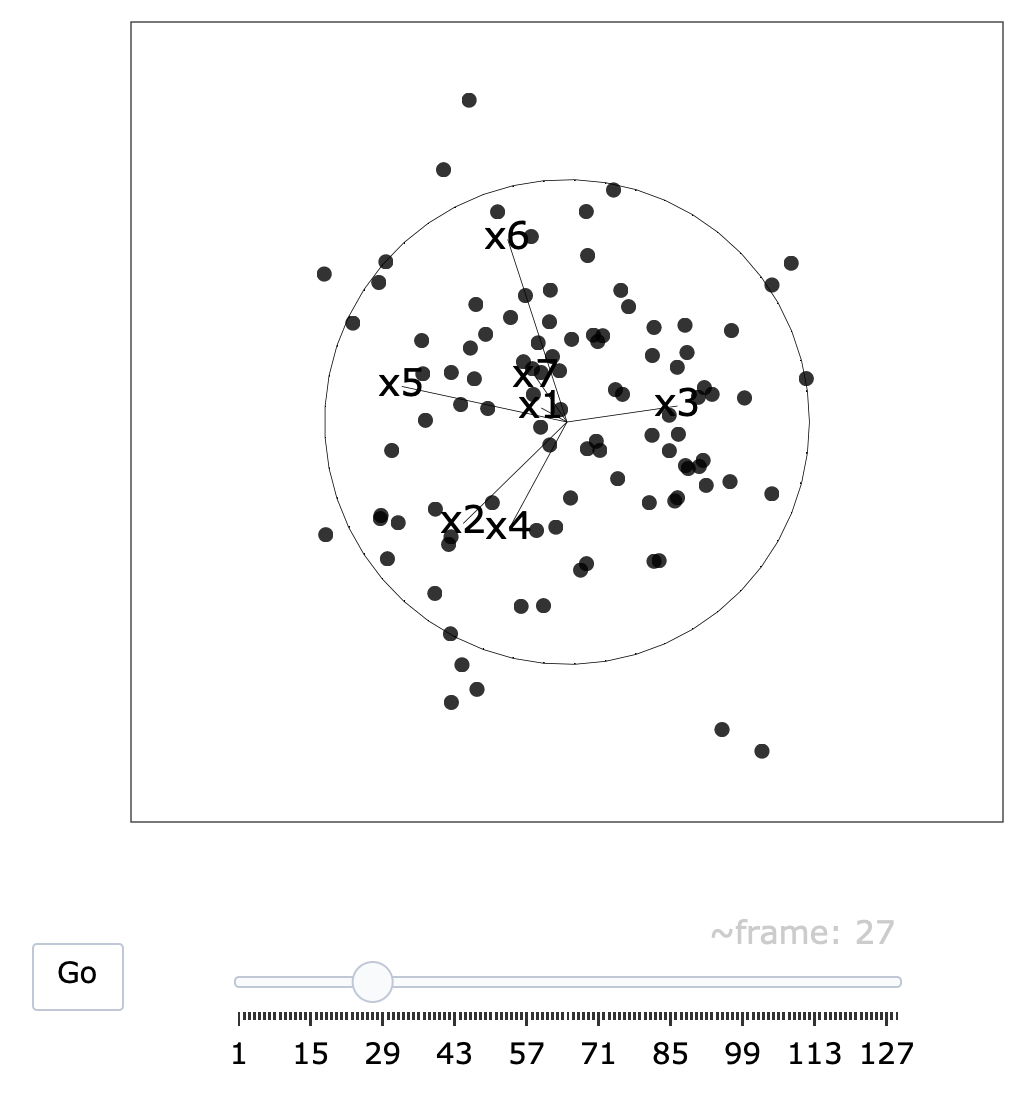
\includegraphics[width=2.08333in,height=\textheight]{images/plane_noise2.png}

}

}

\end{minipage}%

\caption{\label{fig-plane-noise-pdf}Two frames from a grand tour of the
plane with two additional dimensions of pure noise
(\href{https://dicook.github.io/mulgar_book/3-intro-dimred.html}{can be
viewed here}). The collapsing of the points indicates that this is not
fully 7D. This only happens when any of x1-x5 are contributing strongly
(frame 49 x4, x5; frame 79 x1; frame 115 x2, x3). If x6 or x7 are
contributing strongly the data is spread out fully (frames 27, 96). This
tells us that x6 and x7 are not linearly associated, but other variables
are.}

\end{figure}

\infobox{To determine which variables are responsible for the reduced dimension look for the axes that extend out of the point cloud. These contribute to smaller variation in the observations, and thus indicate dimension reduction.}

The simulated data here is very simple, and what we have learned from
the tour could also be learned from principal component analysis.
However, if there are small complications, such as outliers or nonlinear
relationships, that might not be visible from principal component
analysis, the tour can help you to see them.

Figure~\ref{fig-plane-noise-outlier} and
Figure~\ref{fig-outlier-nonlin-pdf}(a) show example data with an outlier
and Figure~\ref{fig-outlier-nonlin-pdf}(b) shows data with non-linear
relationships.

\begin{Shaded}
\begin{Highlighting}[]
\CommentTok{\# Add several outliers to the plane\_noise data}
\NormalTok{plane\_noise\_outliers }\OtherTok{\textless{}{-}}\NormalTok{ plane\_noise}
\NormalTok{plane\_noise\_outliers[}\DecValTok{101}\NormalTok{,] }\OtherTok{\textless{}{-}} \FunctionTok{c}\NormalTok{(}\DecValTok{2}\NormalTok{, }\DecValTok{2}\NormalTok{, }\SpecialCharTok{{-}}\DecValTok{2}\NormalTok{, }\DecValTok{0}\NormalTok{, }\DecValTok{0}\NormalTok{, }\DecValTok{0}\NormalTok{, }\DecValTok{0}\NormalTok{)}
\NormalTok{plane\_noise\_outliers[}\DecValTok{102}\NormalTok{,] }\OtherTok{\textless{}{-}} \FunctionTok{c}\NormalTok{(}\DecValTok{0}\NormalTok{, }\DecValTok{0}\NormalTok{, }\DecValTok{0}\NormalTok{,}\SpecialCharTok{{-}}\DecValTok{2}\NormalTok{, }\SpecialCharTok{{-}}\DecValTok{2}\NormalTok{, }\DecValTok{0}\NormalTok{, }\DecValTok{0}\NormalTok{)}

\FunctionTok{ggscatmat}\NormalTok{(plane\_noise\_outliers, }\AttributeTok{columns =} \DecValTok{1}\SpecialCharTok{:}\DecValTok{5}\NormalTok{) }\SpecialCharTok{+}
  \FunctionTok{theme}\NormalTok{(}\AttributeTok{aspect.ratio=}\DecValTok{1}\NormalTok{,}
    \AttributeTok{panel.background =} 
          \FunctionTok{element\_rect}\NormalTok{(}\AttributeTok{colour=}\StringTok{"black"}\NormalTok{, }\AttributeTok{fill=}\ConstantTok{NA}\NormalTok{),}
    \AttributeTok{axis.text =} \FunctionTok{element\_blank}\NormalTok{(),}
    \AttributeTok{axis.ticks =} \FunctionTok{element\_blank}\NormalTok{())}
\end{Highlighting}
\end{Shaded}

\begin{figure}[H]

{\centering 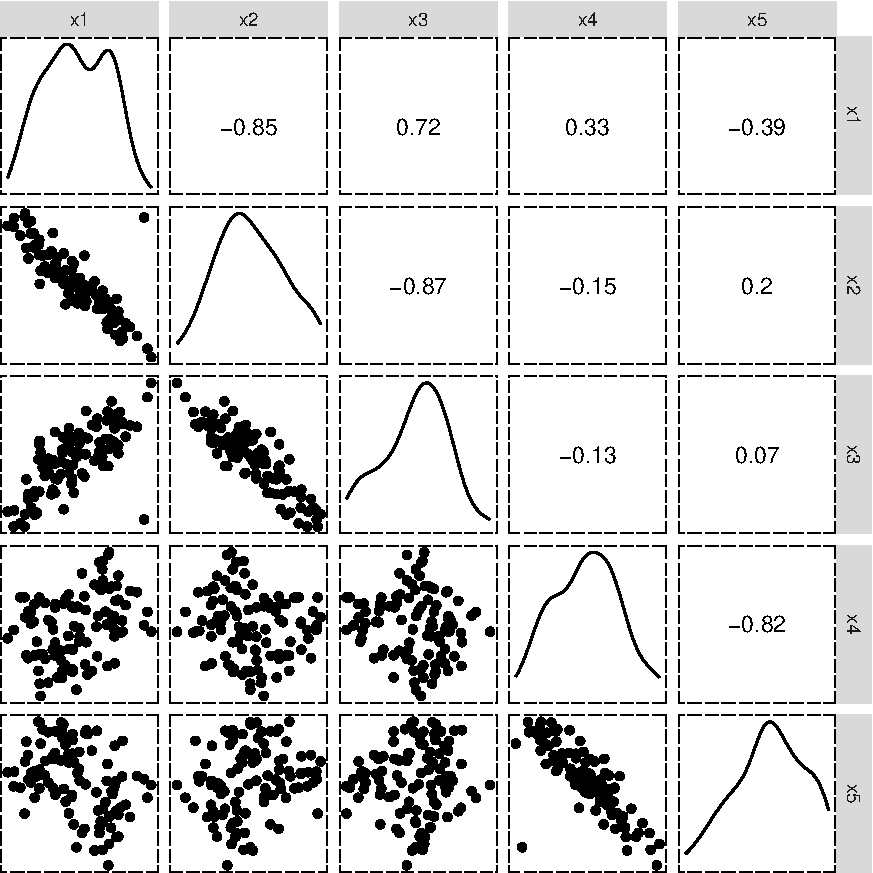
\includegraphics[width=0.8\textwidth,height=\textheight]{3-intro-dimred_files/figure-pdf/fig-plane-noise-outlier-1.pdf}

}

\caption{\label{fig-plane-noise-outlier}Scatterplot matrix of the plane
with noise data, with two added outliers in variables with strong
correlation.}

\end{figure}

\begin{Shaded}
\begin{Highlighting}[]
\FunctionTok{render\_gif}\NormalTok{(plane\_noise\_outliers,          }
           \FunctionTok{grand\_tour}\NormalTok{(), }
           \FunctionTok{display\_xy}\NormalTok{(),}
           \AttributeTok{gif\_file=}\StringTok{"gifs/pn\_outliers.gif"}\NormalTok{,}
           \AttributeTok{frames=}\DecValTok{500}\NormalTok{,}
           \AttributeTok{width=}\DecValTok{200}\NormalTok{,}
           \AttributeTok{height=}\DecValTok{200}\NormalTok{)}

\FunctionTok{data}\NormalTok{(plane\_nonlin)}
\FunctionTok{render\_gif}\NormalTok{(plane\_nonlin,          }
           \FunctionTok{grand\_tour}\NormalTok{(), }
           \FunctionTok{display\_xy}\NormalTok{(),}
           \AttributeTok{gif\_file=}\StringTok{"gifs/plane\_nonlin.gif"}\NormalTok{,}
           \AttributeTok{frames=}\DecValTok{500}\NormalTok{,}
           \AttributeTok{width=}\DecValTok{200}\NormalTok{,}
           \AttributeTok{height=}\DecValTok{200}\NormalTok{)}
\end{Highlighting}
\end{Shaded}

\begin{figure}

\begin{minipage}[t]{0.50\linewidth}

{\centering 

\raisebox{-\height}{

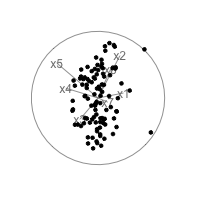
\includegraphics[width=2.08333in,height=\textheight]{images/pn_outliers.png}

}

}

\subcaption{\label{fig-outlier}Outliers}
\end{minipage}%
%
\begin{minipage}[t]{0.50\linewidth}

{\centering 

\raisebox{-\height}{

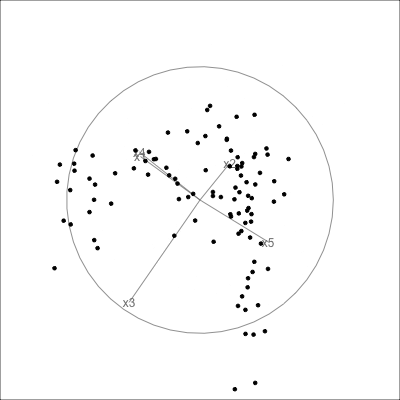
\includegraphics[width=2.08333in,height=\textheight]{images/plane_nonlin.png}

}

}

\subcaption{\label{fig-nonlinear}Non-linear relationship}
\end{minipage}%

\caption{\label{fig-outlier-nonlin-pdf}Two frames from tours of examples
of different types of dimensionality issues: outliers (a) and
non-linearity (b). In (a) you can see two points far from the others in
the projection. During a tour the two can be seen with different
movement patterns -- moving faster and in different directions than
other points. Outliers will affect detection of reduced dimension, but
they can be ignored when assessing dimensionality with the tour. In (b)
there is a non-linear relationship between several variables, primarily
with x3. Non-linear relationships may not be easily captured by other
techniques but are often visible with the tour. (The tours can be viewed
\href{https://dicook.github.io/mulgar_book/3-intro-dimred.html}{here}.)}

\end{figure}

\hypertarget{exercises-2}{%
\section*{Exercises}\label{exercises-2}}
\addcontentsline{toc}{section}{Exercises}

\markright{Exercises}

\begin{enumerate}
\def\labelenumi{\arabic{enumi}.}
\tightlist
\item
  Multicollinearity is when the predictors for a model are strongly
  linearly associated. It can adversely affect the fitting of most
  models, because many possible models may be equally as good. Variable
  importance might be masked by correlated variables, and confidence
  intervals generated for linear models might be too wide. Check the for
  multicollinearity or other associations between the predictors in:
\end{enumerate}

\begin{enumerate}
\def\labelenumi{\alph{enumi}.}
\tightlist
\item
  2001 Australian election data
\item
  2016 Australian election data
\end{enumerate}

\begin{enumerate}
\def\labelenumi{\arabic{enumi}.}
\setcounter{enumi}{1}
\tightlist
\item
  Examine 5D multivariate normal samples drawn from populations with a
  range of variance-covariance matrices. (You can use the
  \texttt{mvtnorm} package to do the sampling, for example.) Examine the
  data using a grand tour. What changes when you change the correlation
  from close to zero to close to 1? Can you see a difference between
  strong positive correlation and strong negative correlation?
\end{enumerate}

\hypertarget{principal-component-analysis}{%
\chapter{Principal component
analysis}\label{principal-component-analysis}}

Reducing dimensionality using principal component analysis (PCA) dates
back to Pearson (1901) and Hotelling (1933), and Jolliffe \& Cadima
(2016) provides a current overview. The goal is to find a smaller set of
variables, \(q (< p)\), that contain as much information as the original
as possible. The new set of variables, known as principal components
(PCs), are linear combinations of the original variables. The PCs can be
used to represent the data in a lower-dimensional space.

The process is essentially an optimisation procedure, although PCA has
an analytical solution. It solves the problem of

\[
\max_{a_k} ~\text{Var} (Xa_k),
\] where \(X\) is the \(n \times p\) data matrix, \(a_k (k=1, ..., p)\)
is a 1D projection vector, called an eigenvector, and the
\(\text{Var} (Xa_k)\) is called an eigenvalue. So PCA is a sequential
process, that will find the direction in the high-dimensional space (as
given by the first eigenvector) where the data is most varied, and then
find the second most varied direction, and so on. The eigenvectors
define the combination of the original variables, and the eigenvalues
define the amount of variance explained by the reduced number of
variables.

PCA is very broadly useful for summarising linear association by using
combinations of variables that are highly correlated. However, high
correlation can also occur when there are outliers, or clustering. PCA
is commonly used to detect these patterns also.

\infobox{With visualisation we want to assess whether it is appropriate to use PCA to summarise any linear association by using combinations of variables that are highly correlated. It can help to detect other patterns that might affect the PCA results such as outliers, clustering or non-linear dependence.}

PCA is not very effective when the distribution of the variables is
highly skewed, so it can be helpful to transform variables to make them
more symmetrically distributed before conducting PCA. It is also
possible to summarise different types of structure by generalising the
optimisation criteria to any function of projected data, \(f(XA)\),
which is called \emph{projection pursuit} (PP). PP has a long history
(Kruskal (1964a), Friedman \& Tukey (1974), Diaconis \& Freedman
(1984b), Jones \& Sibson (1987), Huber (1985)), and there are regularly
new developments (e.g. E.-K. Lee \& Cook (2009), Perisic \& Posse
(2005), Y. D. Lee et al. (2013), Loperfido (2018), Bickel et al. (2018),
C. Zhang et al. (2023)).

\hypertarget{determining-how-many-dimensions}{%
\section{Determining how many
dimensions}\label{determining-how-many-dimensions}}

We would start by examining the data using a grand tour. The goal is to
check whether there might be potential issues for PCA, such as skewness,
outliers or clustering, or even non-linear dependencies.

We'll start be showing PCA on the simulated data from
Chapter~\ref{sec-dimension-overview}. The scree plots show that PCA
supports that the data are 2D, 3D and 5D respectively.

\begin{Shaded}
\begin{Highlighting}[]
\FunctionTok{library}\NormalTok{(dplyr)}
\FunctionTok{library}\NormalTok{(ggplot2)}
\FunctionTok{library}\NormalTok{(mulgar)}
\FunctionTok{data}\NormalTok{(plane)}
\FunctionTok{data}\NormalTok{(box)}
\FunctionTok{library}\NormalTok{(geozoo)}
\NormalTok{cube5d }\OtherTok{\textless{}{-}} \FunctionTok{data.frame}\NormalTok{(}\FunctionTok{cube.solid.random}\NormalTok{(}\AttributeTok{p=}\DecValTok{5}\NormalTok{, }\AttributeTok{n=}\DecValTok{300}\NormalTok{)}\SpecialCharTok{$}\NormalTok{points)}
\FunctionTok{colnames}\NormalTok{(cube5d) }\OtherTok{\textless{}{-}} \FunctionTok{paste0}\NormalTok{(}\StringTok{"x"}\NormalTok{, }\DecValTok{1}\SpecialCharTok{:}\DecValTok{5}\NormalTok{)}
\NormalTok{cube5d }\OtherTok{\textless{}{-}} \FunctionTok{data.frame}\NormalTok{(}\FunctionTok{apply}\NormalTok{(cube5d, }\DecValTok{2}\NormalTok{, }\ControlFlowTok{function}\NormalTok{(x) (x}\SpecialCharTok{{-}}\FunctionTok{mean}\NormalTok{(x))}\SpecialCharTok{/}\FunctionTok{sd}\NormalTok{(x)))}
\NormalTok{p\_pca }\OtherTok{\textless{}{-}} \FunctionTok{prcomp}\NormalTok{(plane)}
\NormalTok{b\_pca }\OtherTok{\textless{}{-}} \FunctionTok{prcomp}\NormalTok{(box)}
\NormalTok{c\_pca }\OtherTok{\textless{}{-}} \FunctionTok{prcomp}\NormalTok{(cube5d)}
\NormalTok{p\_scree }\OtherTok{\textless{}{-}} \FunctionTok{ggscree}\NormalTok{(p\_pca, }\AttributeTok{q =} \DecValTok{5}\NormalTok{) }\SpecialCharTok{+} \FunctionTok{theme\_minimal}\NormalTok{()}

\NormalTok{b\_scree }\OtherTok{\textless{}{-}} \FunctionTok{ggscree}\NormalTok{(b\_pca, }\AttributeTok{q =} \DecValTok{5}\NormalTok{) }\SpecialCharTok{+} \FunctionTok{theme\_minimal}\NormalTok{()}
\NormalTok{c\_scree }\OtherTok{\textless{}{-}} \FunctionTok{ggscree}\NormalTok{(c\_pca, }\AttributeTok{q =} \DecValTok{5}\NormalTok{) }\SpecialCharTok{+} \FunctionTok{theme\_minimal}\NormalTok{()}
\end{Highlighting}
\end{Shaded}

\begin{figure}

{\centering 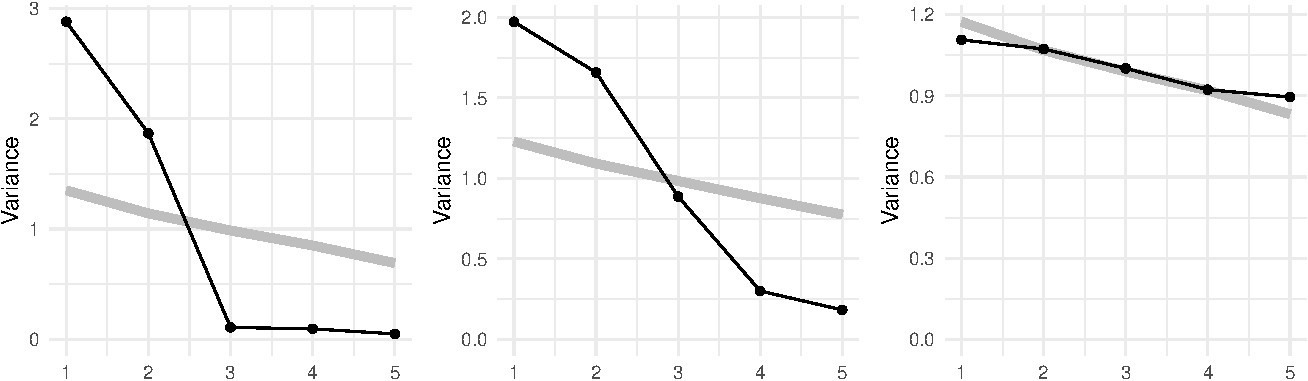
\includegraphics[width=1\textwidth,height=\textheight]{4-pca_files/figure-pdf/fig-2D-pca-1.pdf}

}

\caption{\label{fig-2D-pca}Scree plots for the three simulated data sets
shown in Figure 3.2. The 2D in 5D is clearly recognised by PCA to be 2D
because the variance drops substantially between 2-3 principal
components. The 3D in 5D is possibly 3D because the variance drops from
3-4 principal components. The fully 5D data has no drop in variance, and
all values are close to the typical value one would observe if the data
was fully 5D.}

\end{figure}

The next step is to look at the coefficients for the selected number of
PCs. Table~\ref{tbl-plane-pcs} shows the coefficients for the first two
PCs of the \texttt{plane} data. All five variables contribute, with
\texttt{x1}, \texttt{x2}, \texttt{x3} contributing more to \texttt{PC1},
and \texttt{x4}, \texttt{x5} contributing more to \texttt{PC2}.
Table~\ref{tbl-box-pcs} shows the coefficients for the first three PCs.
Variables \texttt{x1}, \texttt{x2}, \texttt{x3} contribute strongly to
\texttt{PC1}, \texttt{PC2} has contributions from all variables except
\texttt{x3} and variables \texttt{x4} and \texttt{x5} contribute
strongly to \texttt{PC3}.

\begin{Shaded}
\begin{Highlighting}[]
\FunctionTok{library}\NormalTok{(gt)}
\NormalTok{p\_pca}\SpecialCharTok{$}\NormalTok{rotation[,}\DecValTok{1}\SpecialCharTok{:}\DecValTok{2}\NormalTok{] }\SpecialCharTok{\%\textgreater{}\%}
  \FunctionTok{as\_tibble}\NormalTok{(}\AttributeTok{rownames=}\StringTok{"Variable"}\NormalTok{) }\SpecialCharTok{\%\textgreater{}\%} 
  \FunctionTok{gt}\NormalTok{() }\SpecialCharTok{\%\textgreater{}\%}
  \FunctionTok{fmt\_number}\NormalTok{(}\AttributeTok{columns =} \FunctionTok{c}\NormalTok{(PC1, PC2),}
             \AttributeTok{decimals =} \DecValTok{2}\NormalTok{)}
\end{Highlighting}
\end{Shaded}

\hypertarget{tbl-plane-pcs}{}
\begin{longtable}{lrr}
\caption{\label{tbl-plane-pcs}Coefficients for the first two PCs for the plane data. }\tabularnewline

\toprule
Variable & PC1 & PC2 \\ 
\midrule
x1 & $0.58$ & $-0.06$ \\ 
x2 & $-0.55$ & $0.21$ \\ 
x3 & $0.47$ & $-0.41$ \\ 
x4 & $0.25$ & $0.64$ \\ 
x5 & $-0.29$ & $-0.62$ \\ 
\bottomrule
\end{longtable}

\begin{Shaded}
\begin{Highlighting}[]
\NormalTok{b\_pca}\SpecialCharTok{$}\NormalTok{rotation[,}\DecValTok{1}\SpecialCharTok{:}\DecValTok{3}\NormalTok{] }\SpecialCharTok{\%\textgreater{}\%}
  \FunctionTok{as\_tibble}\NormalTok{(}\AttributeTok{rownames=}\StringTok{"Variable"}\NormalTok{) }\SpecialCharTok{\%\textgreater{}\%} 
  \FunctionTok{gt}\NormalTok{() }\SpecialCharTok{\%\textgreater{}\%}
  \FunctionTok{fmt\_number}\NormalTok{(}\AttributeTok{columns =} \FunctionTok{c}\NormalTok{(PC1, PC2, PC3),}
             \AttributeTok{decimals =} \DecValTok{2}\NormalTok{)}
\end{Highlighting}
\end{Shaded}

\hypertarget{tbl-box-pcs}{}
\begin{longtable}{lrrr}
\caption{\label{tbl-box-pcs}Coefficients for the first three PCs for the box data. }\tabularnewline

\toprule
Variable & PC1 & PC2 & PC3 \\ 
\midrule
x1 & $-0.51$ & $0.46$ & $0.11$ \\ 
x2 & $0.51$ & $0.46$ & $0.00$ \\ 
x3 & $-0.65$ & $-0.09$ & $0.23$ \\ 
x4 & $-0.22$ & $0.36$ & $-0.87$ \\ 
x5 & $0.02$ & $0.66$ & $0.43$ \\ 
\bottomrule
\end{longtable}

In each of these simulated data sets, all five variables contributed to
the dimension reduction. If we added two purely noise variables to the
plane data, as done in Chapter~\ref{sec-dimension-overview}, the scree
plot would indicate that the data is now 4D, and we would get a
different interpretation of the coefficients from the PCA. We see that
\texttt{PC1} and \texttt{PC2} are approximately the same as before, with
main variables being (\texttt{x1}, \texttt{x2}, \texttt{x3}) and
(\texttt{x4}, \texttt{x5}) respectively. \texttt{PC3} and \texttt{PC4}
are both \texttt{x6} and \texttt{x7}.

\begin{Shaded}
\begin{Highlighting}[]
\FunctionTok{set.seed}\NormalTok{(}\DecValTok{5143}\NormalTok{)}
\NormalTok{plane\_noise }\OtherTok{\textless{}{-}}\NormalTok{ plane}
\NormalTok{plane\_noise}\SpecialCharTok{$}\NormalTok{x6 }\OtherTok{\textless{}{-}} \FunctionTok{rnorm}\NormalTok{(}\DecValTok{100}\NormalTok{)}
\NormalTok{plane\_noise}\SpecialCharTok{$}\NormalTok{x7 }\OtherTok{\textless{}{-}} \FunctionTok{rnorm}\NormalTok{(}\DecValTok{100}\NormalTok{)}
\NormalTok{plane\_noise }\OtherTok{\textless{}{-}} \FunctionTok{data.frame}\NormalTok{(}\FunctionTok{apply}\NormalTok{(plane\_noise, }\DecValTok{2}\NormalTok{, }\ControlFlowTok{function}\NormalTok{(x) (x}\SpecialCharTok{{-}}\FunctionTok{mean}\NormalTok{(x))}\SpecialCharTok{/}\FunctionTok{sd}\NormalTok{(x)))}

\NormalTok{pn\_pca }\OtherTok{\textless{}{-}} \FunctionTok{prcomp}\NormalTok{(plane\_noise)}
\FunctionTok{ggscree}\NormalTok{(pn\_pca, }\AttributeTok{q =} \DecValTok{7}\NormalTok{) }\SpecialCharTok{+} \FunctionTok{theme\_minimal}\NormalTok{()}
\end{Highlighting}
\end{Shaded}

\begin{figure}[H]

{\centering 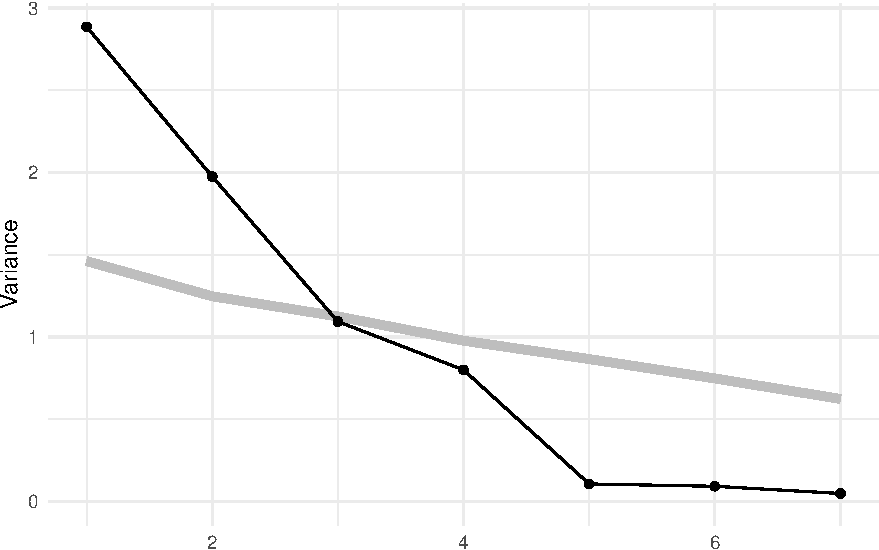
\includegraphics[width=0.8\textwidth,height=\textheight]{4-pca_files/figure-pdf/fig-plane-noise-scree-1.pdf}

}

\caption{\label{fig-plane-noise-scree}Additional noise variables expands
the data to 4D.}

\end{figure}

\begin{Shaded}
\begin{Highlighting}[]
\NormalTok{pn\_pca}\SpecialCharTok{$}\NormalTok{rotation[,}\DecValTok{1}\SpecialCharTok{:}\DecValTok{4}\NormalTok{] }\SpecialCharTok{\%\textgreater{}\%}
  \FunctionTok{as\_tibble}\NormalTok{(}\AttributeTok{rownames=}\StringTok{"Variable"}\NormalTok{) }\SpecialCharTok{\%\textgreater{}\%} 
  \FunctionTok{gt}\NormalTok{() }\SpecialCharTok{\%\textgreater{}\%}
  \FunctionTok{fmt\_number}\NormalTok{(}\AttributeTok{columns =} \FunctionTok{c}\NormalTok{(PC1, PC2, PC3, PC4),}
             \AttributeTok{decimals =} \DecValTok{2}\NormalTok{)}
\end{Highlighting}
\end{Shaded}

\hypertarget{tbl-plane-noise-pcs}{}
\begin{longtable}{lrrrr}
\caption{\label{tbl-plane-noise-pcs}Coefficients for the first four PCs for the box data. }\tabularnewline

\toprule
Variable & PC1 & PC2 & PC3 & PC4 \\ 
\midrule
x1 & $0.58$ & $0.04$ & $0.01$ & $0.00$ \\ 
x2 & $-0.55$ & $-0.18$ & $-0.03$ & $0.07$ \\ 
x3 & $0.47$ & $0.37$ & $0.05$ & $-0.20$ \\ 
x4 & $0.24$ & $-0.62$ & $-0.06$ & $0.17$ \\ 
x5 & $-0.28$ & $0.60$ & $0.07$ & $-0.14$ \\ 
x6 & $0.05$ & $0.29$ & $-0.58$ & $0.76$ \\ 
x7 & $-0.02$ & $-0.08$ & $-0.81$ & $-0.58$ \\ 
\bottomrule
\end{longtable}

\hypertarget{example-pisa}{%
\subsection{Example: pisa}\label{example-pisa}}

The \texttt{pisa} data contains simulated data from math, reading and
science scores, totalling 30 variables. PCA is used here to examine the
association. We might expect that it is 3D, but what we see suggests it
is primarily 1D. This means that a student that scores well in math,
will also score well in reading and science.

\begin{Shaded}
\begin{Highlighting}[]
\FunctionTok{data}\NormalTok{(pisa)}
\NormalTok{pisa\_std }\OtherTok{\textless{}{-}}\NormalTok{ pisa }\SpecialCharTok{\%\textgreater{}\%}
  \FunctionTok{filter}\NormalTok{(CNT }\SpecialCharTok{==} \StringTok{"Australia"}\NormalTok{) }\SpecialCharTok{\%\textgreater{}\%}
  \FunctionTok{select}\NormalTok{(}\SpecialCharTok{{-}}\NormalTok{CNT) }\SpecialCharTok{\%\textgreater{}\%}
  \FunctionTok{mutate\_all}\NormalTok{(mulgar}\SpecialCharTok{:::}\NormalTok{scale2)}
\NormalTok{pisa\_pca }\OtherTok{\textless{}{-}} \FunctionTok{prcomp}\NormalTok{(pisa\_std)}
\NormalTok{pisa\_scree }\OtherTok{\textless{}{-}} \FunctionTok{ggscree}\NormalTok{(pisa\_pca, }\AttributeTok{q =} \DecValTok{15}\NormalTok{) }\SpecialCharTok{+} \FunctionTok{theme\_minimal}\NormalTok{()}
\end{Highlighting}
\end{Shaded}

The scree plot in \textbf{?@fig-pisa-scree} shows a big drop from one to
two PCs in the amount of variance explained. A grand tour on the 30
variables can be run using \texttt{animate\_xy()}:

\begin{Shaded}
\begin{Highlighting}[]
\FunctionTok{animate\_xy}\NormalTok{(pisa\_std, }\AttributeTok{half\_range=}\DecValTok{1}\NormalTok{)}
\end{Highlighting}
\end{Shaded}

or rendered as an animated gif using \texttt{render\_gif()}:

\begin{Shaded}
\begin{Highlighting}[]
\FunctionTok{render\_gif}\NormalTok{(pisa\_std, }
           \FunctionTok{grand\_tour}\NormalTok{(), }
           \FunctionTok{display\_xy}\NormalTok{(}\AttributeTok{half\_range=}\FloatTok{0.9}\NormalTok{),}
           \AttributeTok{gif\_file=}\StringTok{"gifs/pisa\_gt.gif"}\NormalTok{,}
           \AttributeTok{frames=}\DecValTok{500}\NormalTok{,}
           \AttributeTok{width=}\DecValTok{400}\NormalTok{,}
           \AttributeTok{height=}\DecValTok{400}\NormalTok{,}
           \AttributeTok{loop=}\ConstantTok{FALSE}\NormalTok{)}
\end{Highlighting}
\end{Shaded}

and we can see that the data is elliptical in most projections,
sometimes shrinking to be a small circle. This pattern strongly
indicates that there is one primary direction of variation in the data,
with only small variation in any direction away from it. Shrinking to
the small circle is analogous to to how \emph{a pencil or cigar or water
bottle in 3D looks from some angles}.

The coefficients of the first PC (first eigenvector) are roughly equal
in magnitude (as shown below), which tells us that all variables roughly
contribute. Interestingly, they are all negative, which is not actually
meaningful. With different software these could easily have been all
positive. The sign of the coefficients can be reversed, as long as all
are reversed, which is the same as an arrow pointing one way, changing
and pointing the other way.

\begin{Shaded}
\begin{Highlighting}[]
\FunctionTok{round}\NormalTok{(pisa\_pca}\SpecialCharTok{$}\NormalTok{rotation[,}\DecValTok{1}\NormalTok{], }\DecValTok{2}\NormalTok{)}
\end{Highlighting}
\end{Shaded}

\begin{verbatim}
 PV1MATH  PV2MATH  PV3MATH  PV4MATH  PV5MATH  PV6MATH 
   -0.18    -0.18    -0.18    -0.18    -0.18    -0.18 
 PV7MATH  PV8MATH  PV9MATH PV10MATH  PV1READ  PV2READ 
   -0.18    -0.18    -0.18    -0.18    -0.19    -0.18 
 PV3READ  PV4READ  PV5READ  PV6READ  PV7READ  PV8READ 
   -0.19    -0.19    -0.19    -0.19    -0.19    -0.19 
 PV9READ PV10READ  PV1SCIE  PV2SCIE  PV3SCIE  PV4SCIE 
   -0.19    -0.19    -0.18    -0.18    -0.19    -0.18 
 PV5SCIE  PV6SCIE  PV7SCIE  PV8SCIE  PV9SCIE PV10SCIE 
   -0.19    -0.18    -0.19    -0.18    -0.19    -0.18 
\end{verbatim}

\insightbox{The tour verifies that the `pisa` data is primarily 1D, indicating that a student who scores well in math, probably scores well in reading and science, too. More interestingly, the regular shape of the data strongly indicates that it is "synthetic", simulated rather than observed.}

\hypertarget{example-aflw}{%
\subsection{Example: aflw}\label{example-aflw}}

This data has player statistics for all the matches in the 2021 season.
We would be interested to know which variables contain similar
information, and thus might be combined into single variables. We would
expect that many statistics to group into a few small sets, such as
offensive and defensive skills. We might also expect that some of the
statistics are skewed, most players have low values and just a handful
of players are stellar. It is also possible that there are some extreme
values. These are interesting features, but they will distract from the
main purpose of grouping the statistics. Thus the tour is used to check
for potential problems with the data prior to conducting PCA.

\begin{Shaded}
\begin{Highlighting}[]
\FunctionTok{library}\NormalTok{(tourr)}
\FunctionTok{data}\NormalTok{(aflw)}
\NormalTok{aflw\_std }\OtherTok{\textless{}{-}}\NormalTok{ aflw }\SpecialCharTok{\%\textgreater{}\%}
  \FunctionTok{mutate\_if}\NormalTok{(is.numeric, }\ControlFlowTok{function}\NormalTok{(x) (x}\SpecialCharTok{{-}}
      \FunctionTok{mean}\NormalTok{(x, }\AttributeTok{na.rm=}\ConstantTok{TRUE}\NormalTok{))}\SpecialCharTok{/}
      \FunctionTok{sd}\NormalTok{(x, }\AttributeTok{na.rm=}\ConstantTok{TRUE}\NormalTok{))}
\end{Highlighting}
\end{Shaded}

To look at all of the 29 player statistics in a grand tour.

\begin{Shaded}
\begin{Highlighting}[]
\FunctionTok{animate\_xy}\NormalTok{(aflw\_std[,}\DecValTok{7}\SpecialCharTok{:}\DecValTok{35}\NormalTok{], }\AttributeTok{half\_range=}\FloatTok{0.9}\NormalTok{)}
\FunctionTok{render\_gif}\NormalTok{(aflw\_std[,}\DecValTok{7}\SpecialCharTok{:}\DecValTok{35}\NormalTok{], }
           \FunctionTok{grand\_tour}\NormalTok{(), }
           \FunctionTok{display\_xy}\NormalTok{(}\AttributeTok{half\_range=}\FloatTok{0.9}\NormalTok{),}
           \AttributeTok{gif\_file=}\StringTok{"gifs/aflw\_gt.gif"}\NormalTok{,}
           \AttributeTok{frames=}\DecValTok{500}\NormalTok{,}
           \AttributeTok{loop=}\ConstantTok{FALSE}\NormalTok{)}
\end{Highlighting}
\end{Shaded}

No major surprises! There is a small amount of skewness, and there are
no major outliers. Skewness indicates that most players have reasonably
similar skills (bunching of points), except for some key players (the
moderate outliers). The skewness could be reduced by applying a log or
square root transformation to some variables prior to running the PCA.
However, we elect not to do this because the moderate outliers are of
interest. These correspond to talented players that we'd like to explore
further with the analysis.

Below we have the conventional summary of the PCA, a scree plot showing
the reduction in variance to be explained when each additional PC is
considered. It is also conventional to look at a table summarising the
proportions of variance explained by PCs, but with almost 30 variables
it is easier to make some decision on the number of PCs needed based on
the scree plot.

\begin{Shaded}
\begin{Highlighting}[]
\NormalTok{aflw\_pca }\OtherTok{\textless{}{-}} \FunctionTok{prcomp}\NormalTok{(aflw\_std[,}\DecValTok{7}\SpecialCharTok{:}\DecValTok{35}\NormalTok{], }
               \AttributeTok{scale =} \ConstantTok{FALSE}\NormalTok{, }
               \AttributeTok{retx=}\ConstantTok{TRUE}\NormalTok{)}

\FunctionTok{ggscree}\NormalTok{(aflw\_pca, }\AttributeTok{q =} \DecValTok{29}\NormalTok{) }\SpecialCharTok{+} \FunctionTok{theme\_minimal}\NormalTok{()}
\end{Highlighting}
\end{Shaded}

\begin{figure}[H]

{\centering 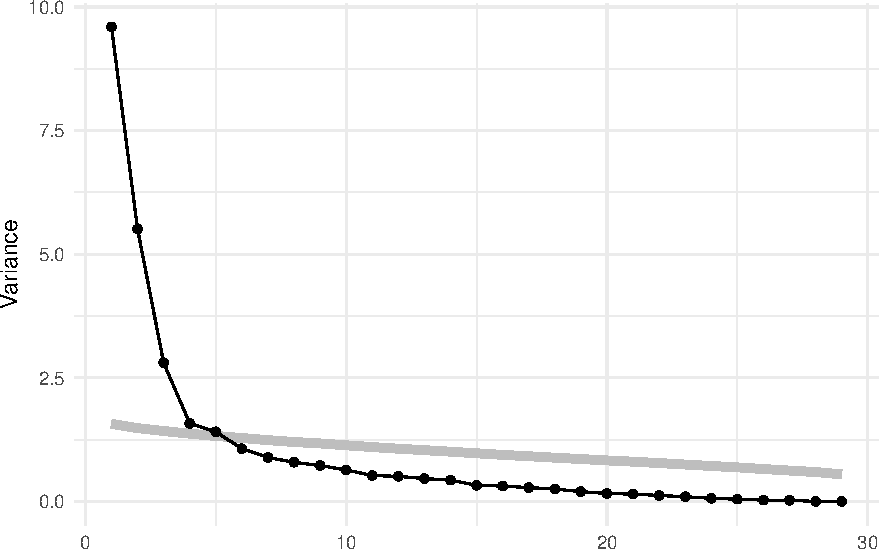
\includegraphics[width=0.8\textwidth,height=\textheight]{4-pca_files/figure-pdf/fig-aflw-pca-1.pdf}

}

\caption{\label{fig-aflw-pca}Scree plot showing decay in variance of
PCs.}

\end{figure}

From the scree plot in Figure~\ref{fig-aflw-pca}, we see a sharp drop
from one to two, two to three and then smaller drops. After four PCs the
variance drops again at six PCs and then gradually decays. We will
choose four PCs to examine more closely. This explains 67.2\% of the
variance.

\begin{Shaded}
\begin{Highlighting}[]
\FunctionTok{library}\NormalTok{(gt)}
\NormalTok{aflw\_pca}\SpecialCharTok{$}\NormalTok{rotation[,}\DecValTok{1}\SpecialCharTok{:}\DecValTok{4}\NormalTok{] }\SpecialCharTok{\%\textgreater{}\%}
  \FunctionTok{as\_tibble}\NormalTok{(}\AttributeTok{rownames=}\StringTok{"Variable"}\NormalTok{) }\SpecialCharTok{\%\textgreater{}\%} 
  \FunctionTok{arrange}\NormalTok{(}\FunctionTok{desc}\NormalTok{(PC1), }\FunctionTok{desc}\NormalTok{(PC2), }\FunctionTok{desc}\NormalTok{(PC3)) }\SpecialCharTok{\%\textgreater{}\%}
  \FunctionTok{gt}\NormalTok{() }\SpecialCharTok{\%\textgreater{}\%}
  \FunctionTok{fmt\_number}\NormalTok{(}\AttributeTok{columns =} \FunctionTok{c}\NormalTok{(PC1, PC2, PC3, PC4),}
             \AttributeTok{decimals =} \DecValTok{2}\NormalTok{)}
\end{Highlighting}
\end{Shaded}

\hypertarget{tbl-aflw-pcs}{}
\begin{longtable}{lrrrr}
\caption{\label{tbl-aflw-pcs}Coefficients for the first four PCs. }\tabularnewline

\toprule
Variable & PC1 & PC2 & PC3 & PC4 \\ 
\midrule
disposals & $0.31$ & $-0.05$ & $-0.03$ & $0.07$ \\ 
possessions & $0.31$ & $-0.03$ & $-0.07$ & $0.09$ \\ 
kicks & $0.29$ & $-0.04$ & $0.09$ & $-0.12$ \\ 
metres & $0.28$ & $-0.03$ & $0.10$ & $-0.15$ \\ 
contested & $0.28$ & $0.01$ & $-0.12$ & $0.23$ \\ 
uncontested & $0.28$ & $-0.06$ & $-0.01$ & $-0.05$ \\ 
turnovers & $0.27$ & $-0.01$ & $-0.01$ & $-0.29$ \\ 
clearances & $0.23$ & $0.00$ & $-0.29$ & $0.19$ \\ 
clangers & $0.23$ & $-0.02$ & $-0.06$ & $-0.33$ \\ 
handballs & $0.23$ & $-0.04$ & $-0.19$ & $0.31$ \\ 
frees\_for & $0.21$ & $0.02$ & $-0.13$ & $0.18$ \\ 
marks & $0.21$ & $0.03$ & $0.32$ & $0.02$ \\ 
tackles & $0.20$ & $0.01$ & $-0.28$ & $0.09$ \\ 
time\_pct & $0.16$ & $-0.04$ & $0.35$ & $-0.02$ \\ 
intercepts & $0.13$ & $-0.28$ & $0.24$ & $0.03$ \\ 
rebounds\_in50 & $0.13$ & $-0.28$ & $0.24$ & $-0.06$ \\ 
frees\_against & $0.13$ & $0.03$ & $-0.16$ & $-0.23$ \\ 
assists & $0.09$ & $0.23$ & $0.00$ & $0.05$ \\ 
bounces & $0.09$ & $0.03$ & $0.02$ & $-0.28$ \\ 
behinds & $0.09$ & $0.32$ & $0.08$ & $-0.02$ \\ 
shots & $0.08$ & $0.38$ & $0.12$ & $-0.03$ \\ 
tackles\_in50 & $0.07$ & $0.27$ & $-0.18$ & $0.03$ \\ 
marks\_in50 & $0.06$ & $0.34$ & $0.18$ & $0.04$ \\ 
contested\_marks & $0.05$ & $0.16$ & $0.34$ & $0.15$ \\ 
goals & $0.04$ & $0.37$ & $0.16$ & $0.03$ \\ 
accuracy & $0.04$ & $0.34$ & $0.10$ & $0.06$ \\ 
one\_pct & $0.03$ & $-0.21$ & $0.33$ & $0.08$ \\ 
disposal & $0.02$ & $-0.13$ & $0.20$ & $0.50$ \\ 
hitouts & $-0.04$ & $0.00$ & $-0.03$ & $0.32$ \\ 
\bottomrule
\end{longtable}

When there are as many variables as this, it can be hard to digest the
combinations of variables most contributing to each PC. Rearranging the
table by sorting on a selected PC can help. Table~\ref{tbl-aflw-pcs} has
been sorted according to the PC 1 coefficients.

PC 1 is primarily composed of \texttt{disposals}, \texttt{possessions},
\texttt{kicks}, \texttt{metres}, \texttt{uncontested},
\texttt{contested}, \ldots. Actually almost all variables positively
contribute, albeit in different amounts! It is quite common in PCA for
the first PC to be a combination of all variables, although it might
commonly be a closer to equal contribution, and it tells us that there
is one main direction of variation in the data. For PC 1 in the
\texttt{aflw} data, PCA is telling us that the primary variation is
through a combination of skills, and this maps to basic football playing
skills, where some skills (e.g.~disposals, possessions, kicks, \ldots)
are more important.

Thus the second PC might be the more interesting. PC 2 is primarily a
combination of \texttt{shots}, \texttt{goals}, \texttt{marks\_in50},
\texttt{accuracy}, and \texttt{behinds} contrasted against
\texttt{rebounds\_in50} and \texttt{intercepts}. The negative
coefficients are primary offensive skills and the positive coefficients
are defensive skills. This PC is reasonable measure of the offensive vs
defensive skills of a player.

We would continue to interpret each PC by examining large coefficients
to help decide how many PCs are a suitable summary of the information in
the data. Briefly, PC 3 is a measure of worth of the player because
\texttt{time\_pct} has a large coefficient, so players that are on the
field longer will contribute strongly to this new variable. It also has
large (and opposite) contributions from \texttt{clearances},
\texttt{tackles}, \texttt{contested\_marks}. PC 4 appears to be related
to aggressive play with \texttt{clangers}, \texttt{turnovers},
\texttt{bounces} and \texttt{frees\_against} featuring. So all four PCs
have useful information. (Note, if we had continued to examine large
coefficients on PC 5 we would find that all variables already have had
reasonably large coefficients on PC 1-4, which supports restricting
attention to the first four.)

Ideally, when we tour the four PCs, we'd like to be able to stop and
identify players. This involves creating a pre-computed animation, with
additional mouse-over. This is only feasible with a small number of
observations, like the \texttt{aflw} data, because all of the animation
frames are constructed in a single object and passed to \texttt{plotly}.
This object gets large very quickly!

\begin{Shaded}
\begin{Highlighting}[]
\FunctionTok{library}\NormalTok{(plotly)}
\FunctionTok{library}\NormalTok{(htmlwidgets)}
\FunctionTok{set.seed}\NormalTok{(}\DecValTok{20}\NormalTok{)}
\NormalTok{b }\OtherTok{\textless{}{-}} \FunctionTok{basis\_random}\NormalTok{(}\DecValTok{4}\NormalTok{, }\DecValTok{2}\NormalTok{)}
\NormalTok{aflw\_pct }\OtherTok{\textless{}{-}}\NormalTok{ tourr}\SpecialCharTok{::}\FunctionTok{save\_history}\NormalTok{(aflw\_pca}\SpecialCharTok{$}\NormalTok{x[,}\DecValTok{1}\SpecialCharTok{:}\DecValTok{4}\NormalTok{], }
                    \AttributeTok{tour\_path =} \FunctionTok{grand\_tour}\NormalTok{(),}
                    \AttributeTok{start =}\NormalTok{ b,}
                    \AttributeTok{max\_bases =} \DecValTok{5}\NormalTok{)}
\CommentTok{\# To reconstruct projected data plots, later}
\FunctionTok{save}\NormalTok{(aflw\_pct, }\AttributeTok{file=}\StringTok{"data/aflw\_pct.rda"}\NormalTok{) }
\NormalTok{aflw\_pcti }\OtherTok{\textless{}{-}} \FunctionTok{interpolate}\NormalTok{(aflw\_pct, }\FloatTok{0.1}\NormalTok{)}
\NormalTok{aflw\_anim }\OtherTok{\textless{}{-}} \FunctionTok{render\_anim}\NormalTok{(aflw\_pca}\SpecialCharTok{$}\NormalTok{x[,}\DecValTok{1}\SpecialCharTok{:}\DecValTok{4}\NormalTok{],}
                         \AttributeTok{frames=}\NormalTok{aflw\_pcti, }
             \AttributeTok{obs\_labels=}\FunctionTok{paste0}\NormalTok{(aflw}\SpecialCharTok{$}\NormalTok{surname,}
\NormalTok{                               aflw}\SpecialCharTok{$}\NormalTok{given\_name))}

\NormalTok{aflw\_gp }\OtherTok{\textless{}{-}} \FunctionTok{ggplot}\NormalTok{() }\SpecialCharTok{+}
     \FunctionTok{geom\_path}\NormalTok{(}\AttributeTok{data=}\NormalTok{aflw\_anim}\SpecialCharTok{$}\NormalTok{circle, }
               \FunctionTok{aes}\NormalTok{(}\AttributeTok{x=}\NormalTok{c1, }\AttributeTok{y=}\NormalTok{c2,}
                   \AttributeTok{frame=}\NormalTok{frame), }\AttributeTok{linewidth=}\FloatTok{0.1}\NormalTok{) }\SpecialCharTok{+}
     \FunctionTok{geom\_segment}\NormalTok{(}\AttributeTok{data=}\NormalTok{aflw\_anim}\SpecialCharTok{$}\NormalTok{axes, }
                  \FunctionTok{aes}\NormalTok{(}\AttributeTok{x=}\NormalTok{x1, }\AttributeTok{y=}\NormalTok{y1, }
                      \AttributeTok{xend=}\NormalTok{x2, }\AttributeTok{yend=}\NormalTok{y2, }
                      \AttributeTok{frame=}\NormalTok{frame), }
                  \AttributeTok{linewidth=}\FloatTok{0.1}\NormalTok{) }\SpecialCharTok{+}
     \FunctionTok{geom\_text}\NormalTok{(}\AttributeTok{data=}\NormalTok{aflw\_anim}\SpecialCharTok{$}\NormalTok{axes, }
               \FunctionTok{aes}\NormalTok{(}\AttributeTok{x=}\NormalTok{x2, }\AttributeTok{y=}\NormalTok{y2, }
                   \AttributeTok{frame=}\NormalTok{frame, }
                   \AttributeTok{label=}\NormalTok{axis\_labels), }
               \AttributeTok{size=}\DecValTok{5}\NormalTok{) }\SpecialCharTok{+}
     \FunctionTok{geom\_point}\NormalTok{(}\AttributeTok{data=}\NormalTok{aflw\_anim}\SpecialCharTok{$}\NormalTok{frames, }
                \FunctionTok{aes}\NormalTok{(}\AttributeTok{x=}\NormalTok{P1, }\AttributeTok{y=}\NormalTok{P2, }
                    \AttributeTok{frame=}\NormalTok{frame, }
                    \AttributeTok{label=}\NormalTok{obs\_labels), }
                \AttributeTok{alpha=}\FloatTok{0.8}\NormalTok{) }\SpecialCharTok{+}
     \FunctionTok{xlim}\NormalTok{(}\SpecialCharTok{{-}}\DecValTok{1}\NormalTok{,}\DecValTok{1}\NormalTok{) }\SpecialCharTok{+} \FunctionTok{ylim}\NormalTok{(}\SpecialCharTok{{-}}\DecValTok{1}\NormalTok{,}\DecValTok{1}\NormalTok{) }\SpecialCharTok{+}
     \FunctionTok{coord\_equal}\NormalTok{() }\SpecialCharTok{+}
     \FunctionTok{theme\_bw}\NormalTok{() }\SpecialCharTok{+}
     \FunctionTok{theme}\NormalTok{(}\AttributeTok{axis.text=}\FunctionTok{element\_blank}\NormalTok{(),}
         \AttributeTok{axis.title=}\FunctionTok{element\_blank}\NormalTok{(),}
         \AttributeTok{axis.ticks=}\FunctionTok{element\_blank}\NormalTok{(),}
         \AttributeTok{panel.grid=}\FunctionTok{element\_blank}\NormalTok{())}
\NormalTok{aflw\_pctour }\OtherTok{\textless{}{-}} \FunctionTok{ggplotly}\NormalTok{(aflw\_gp,}
                        \AttributeTok{width=}\DecValTok{500}\NormalTok{,}
                        \AttributeTok{height=}\DecValTok{550}\NormalTok{) }\SpecialCharTok{\%\textgreater{}\%}
       \FunctionTok{animation\_button}\NormalTok{(}\AttributeTok{label=}\StringTok{"Go"}\NormalTok{) }\SpecialCharTok{\%\textgreater{}\%}
       \FunctionTok{animation\_slider}\NormalTok{(}\AttributeTok{len=}\FloatTok{0.8}\NormalTok{, }\AttributeTok{x=}\FloatTok{0.5}\NormalTok{,}
                        \AttributeTok{xanchor=}\StringTok{"center"}\NormalTok{) }\SpecialCharTok{\%\textgreater{}\%}
       \FunctionTok{animation\_opts}\NormalTok{(}\AttributeTok{easing=}\StringTok{"linear"}\NormalTok{, }\AttributeTok{transition =} \DecValTok{0}\NormalTok{)}

\NormalTok{htmlwidgets}\SpecialCharTok{::}\FunctionTok{saveWidget}\NormalTok{(aflw\_pctour,}
          \AttributeTok{file=}\StringTok{"html/aflw\_pca.html"}\NormalTok{,}
          \AttributeTok{selfcontained =} \ConstantTok{TRUE}\NormalTok{)}
\end{Highlighting}
\end{Shaded}

From \textbf{?@fig-aflw-pcatour} the shape of the four PCs is similar to
that of all the variables, bunching of points in the centre with a lot
of moderate outliers.

\begin{Shaded}
\begin{Highlighting}[]
\FunctionTok{library}\NormalTok{(plotly)}
\FunctionTok{load}\NormalTok{(}\StringTok{"data/aflw\_pct.rda"}\NormalTok{)}
\NormalTok{aflw\_pcti }\OtherTok{\textless{}{-}} \FunctionTok{interpolate}\NormalTok{(aflw\_pct, }\FloatTok{0.1}\NormalTok{)}
\NormalTok{f18 }\OtherTok{\textless{}{-}} \FunctionTok{matrix}\NormalTok{(aflw\_pcti[,,}\DecValTok{18}\NormalTok{], }\AttributeTok{ncol=}\DecValTok{2}\NormalTok{)}
\NormalTok{p18 }\OtherTok{\textless{}{-}} \FunctionTok{render\_proj}\NormalTok{(aflw\_pca}\SpecialCharTok{$}\NormalTok{x[,}\DecValTok{1}\SpecialCharTok{:}\DecValTok{4}\NormalTok{], f18, }
                   \AttributeTok{obs\_labels=}\FunctionTok{paste0}\NormalTok{(aflw}\SpecialCharTok{$}\NormalTok{surname,}
\NormalTok{                               aflw}\SpecialCharTok{$}\NormalTok{given\_name))}
\NormalTok{pg18 }\OtherTok{\textless{}{-}} \FunctionTok{ggplot}\NormalTok{() }\SpecialCharTok{+}
  \FunctionTok{geom\_path}\NormalTok{(}\AttributeTok{data=}\NormalTok{p18}\SpecialCharTok{$}\NormalTok{circle, }\FunctionTok{aes}\NormalTok{(}\AttributeTok{x=}\NormalTok{c1, }\AttributeTok{y=}\NormalTok{c2)) }\SpecialCharTok{+}
  \FunctionTok{geom\_segment}\NormalTok{(}\AttributeTok{data=}\NormalTok{p18}\SpecialCharTok{$}\NormalTok{axes, }\FunctionTok{aes}\NormalTok{(}\AttributeTok{x=}\NormalTok{x1, }\AttributeTok{y=}\NormalTok{y1, }\AttributeTok{xend=}\NormalTok{x2, }\AttributeTok{yend=}\NormalTok{y2)) }\SpecialCharTok{+}
  \FunctionTok{geom\_text}\NormalTok{(}\AttributeTok{data=}\NormalTok{p18}\SpecialCharTok{$}\NormalTok{axes, }\FunctionTok{aes}\NormalTok{(}\AttributeTok{x=}\NormalTok{x2, }\AttributeTok{y=}\NormalTok{y2, }\AttributeTok{label=}\FunctionTok{rownames}\NormalTok{(p18}\SpecialCharTok{$}\NormalTok{axes))) }\SpecialCharTok{+}
  \FunctionTok{geom\_point}\NormalTok{(}\AttributeTok{data=}\NormalTok{p18}\SpecialCharTok{$}\NormalTok{data\_prj, }\FunctionTok{aes}\NormalTok{(}\AttributeTok{x=}\NormalTok{P1, }\AttributeTok{y=}\NormalTok{P2, }\AttributeTok{label=}\NormalTok{obs\_labels)) }\SpecialCharTok{+}
  \FunctionTok{xlim}\NormalTok{(}\SpecialCharTok{{-}}\DecValTok{1}\NormalTok{,}\DecValTok{1}\NormalTok{) }\SpecialCharTok{+} \FunctionTok{ylim}\NormalTok{(}\SpecialCharTok{{-}}\DecValTok{1}\NormalTok{, }\DecValTok{1}\NormalTok{) }\SpecialCharTok{+}
  \CommentTok{\#ggtitle("Frame 18") +}
  \FunctionTok{theme\_bw}\NormalTok{() }\SpecialCharTok{+}
  \FunctionTok{theme}\NormalTok{(}
    \AttributeTok{axis.text=}\FunctionTok{element\_blank}\NormalTok{(),}
    \AttributeTok{axis.title=}\FunctionTok{element\_blank}\NormalTok{(),}
    \AttributeTok{axis.ticks=}\FunctionTok{element\_blank}\NormalTok{(),}
    \AttributeTok{panel.grid=}\FunctionTok{element\_blank}\NormalTok{())}
\FunctionTok{ggplotly}\NormalTok{(pg18, }\AttributeTok{width=}\DecValTok{500}\NormalTok{, }\AttributeTok{height=}\DecValTok{500}\NormalTok{)}
\end{Highlighting}
\end{Shaded}

\begin{figure}[H]

{\centering 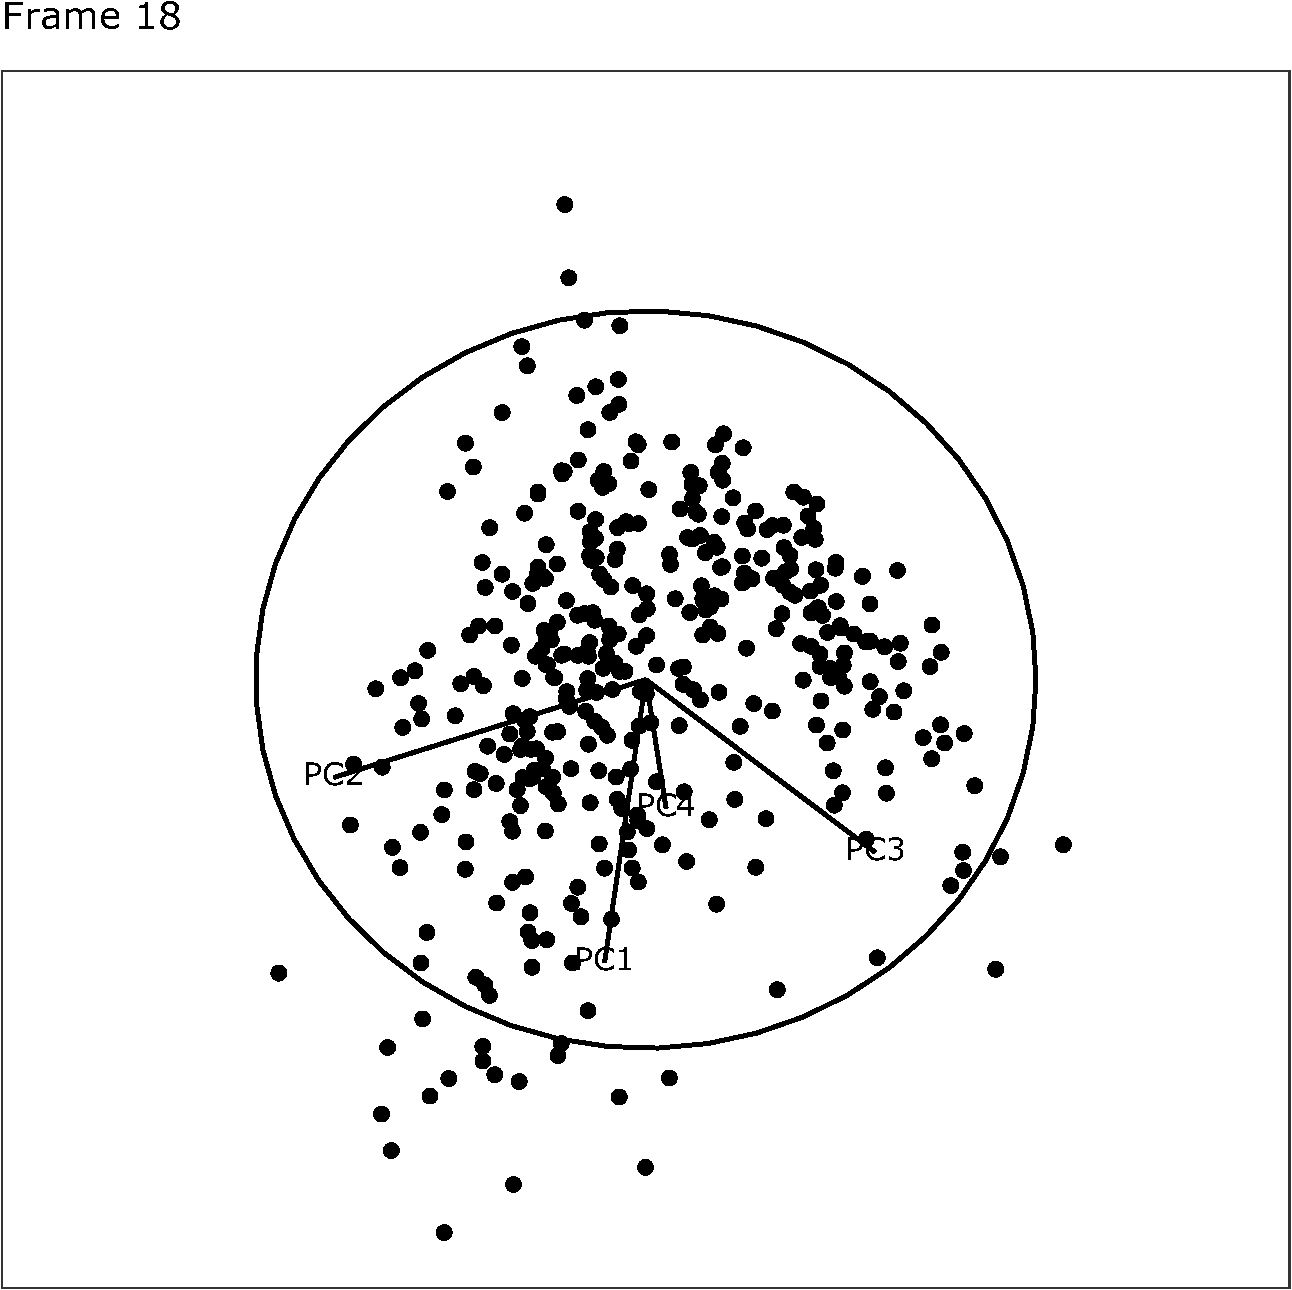
\includegraphics[width=0.8\textwidth,height=\textheight]{4-pca_files/figure-pdf/fig-aflw-pcaplots-1.pdf}

}

\caption{\label{fig-aflw-pcaplots}Frame 18 re-plotted so that players
can be identified on mouse-over.}

\end{figure}

For any particular frame, like 18 re-plotted in
Figure~\ref{fig-aflw-pcaplots}, we can investigate further. Here there
is a branching pattern, where the branch points in the direction of PC
1. Mouse-over the players at the tip of this branch and we find players
like Alyce Parker, Brittany Bonnici, Dana Hooker, Kiara Bowers. If you
look up the bios of these players you'll find they all have generally
good player descriptions like ``elite disposals'', ``powerful left
foot'', ``hard-running midfielder'', ``best and fairest''.

In the direction of PC 2, you'll find players like Lauren Ahrens, Stacey
Livingstone who are star defenders. Players in this end of PC 1, have
high scores on \texttt{intercepts} and \texttt{rebounds\_in50}.

Another interesting frame for inspecting PC 2 is 59. PC 2 at one end has
players with high goal scoring skills, and the other good defending
skills. So mousing over the other end of PC 2 finds players like Gemma
Houghton and Katie Brennan who are known for their goal scoring. The
branch pattern is an interesting one, because it tells us there is some
combination of skills that are lacking among all players, primarily this
appears to be there some distinction between defenders skills and
general playing skills. It's not as simple as this because the branching
is only visible when PC 1 and PC 2 are examined with PC 3.

PCA is useful for getting a sense of the variation in a high-dimensional
data set. Interpreting the principal components is often useful, but it
can be discombobulating. For the \texttt{aflw} data it would be good to
think about it as a guide to the main directions of variation and to
follow with a more direct engineering of variables into interesting
player characteristics. For example, calculate offensive skill as an
equal combination of goals, accuracy, shots, behinds. A set of new
variables specifically computed to measure particular skills would make
explaining an analysis easier.

\hypertarget{examining-the-pca-model-in-the-data-space}{%
\section{Examining the PCA model in the data
space}\label{examining-the-pca-model-in-the-data-space}}

When you choose a smaller number of PCs \((k)\) than the number of
original variables, this is essentially producing a model for the data.
The model is the lower dimensional \(k\)-D space. It is analogous to a
linear regression model, except that the residuals from the model are
\((p-k)\)-D.

It is common to show the model, that is the data projected into the
\(k\)-D model space. When \(k=2\) this is called a ``biplot''. For the
\texttt{plane} and \texttt{plane\_noise} data the biplots are shown in
Figure~\ref{fig-plane-biplot}. This is useful for checking which
variables contribute most to the new principal component variables, and
also to check for any problems that might have affected the fit, such as
outliers, clusters or non-linearity. Interestingly, biplots are
typically only made in 2D, even if the data should be summarised by more
than two PCs. Occasionally you will see the biplot made for PC \(j\) vs
PC \(k\) also. With the \texttt{pca\_tour()} function in the
\texttt{tourr} package you can view a \(k\)-D biplot. This will display
the \(k\) PCs with the axes displaying the original variables, and thus
see their contribution to the PCs.

\begin{Shaded}
\begin{Highlighting}[]
\FunctionTok{library}\NormalTok{(ggfortify)}
\FunctionTok{library}\NormalTok{(patchwork)}
\NormalTok{plane\_pca }\OtherTok{\textless{}{-}} \FunctionTok{prcomp}\NormalTok{(plane)}
\NormalTok{pl1 }\OtherTok{\textless{}{-}} \FunctionTok{autoplot}\NormalTok{(plane\_pca, }\AttributeTok{loadings =} \ConstantTok{TRUE}\NormalTok{, }
         \AttributeTok{loadings.label =} \ConstantTok{TRUE}\NormalTok{) }\SpecialCharTok{+} 
  \FunctionTok{ggtitle}\NormalTok{(}\StringTok{"(a)"}\NormalTok{) }\SpecialCharTok{+}
  \FunctionTok{theme\_minimal}\NormalTok{() }\SpecialCharTok{+} 
  \FunctionTok{theme}\NormalTok{(}\AttributeTok{aspect.ratio=}\DecValTok{1}\NormalTok{)}
\NormalTok{plane\_noise\_pca }\OtherTok{\textless{}{-}} \FunctionTok{prcomp}\NormalTok{(plane\_noise)}
\NormalTok{pl2 }\OtherTok{\textless{}{-}} \FunctionTok{autoplot}\NormalTok{(plane\_noise\_pca, }\AttributeTok{loadings =} \ConstantTok{TRUE}\NormalTok{, }
         \AttributeTok{loadings.label =} \ConstantTok{TRUE}\NormalTok{) }\SpecialCharTok{+} 
  \FunctionTok{ggtitle}\NormalTok{(}\StringTok{"(b)"}\NormalTok{) }\SpecialCharTok{+}
  \FunctionTok{theme\_minimal}\NormalTok{() }\SpecialCharTok{+} 
  \FunctionTok{theme}\NormalTok{(}\AttributeTok{aspect.ratio=}\DecValTok{1}\NormalTok{)}
\NormalTok{pl1 }\SpecialCharTok{+}\NormalTok{ pl2}
\end{Highlighting}
\end{Shaded}

\begin{figure}[H]

{\centering 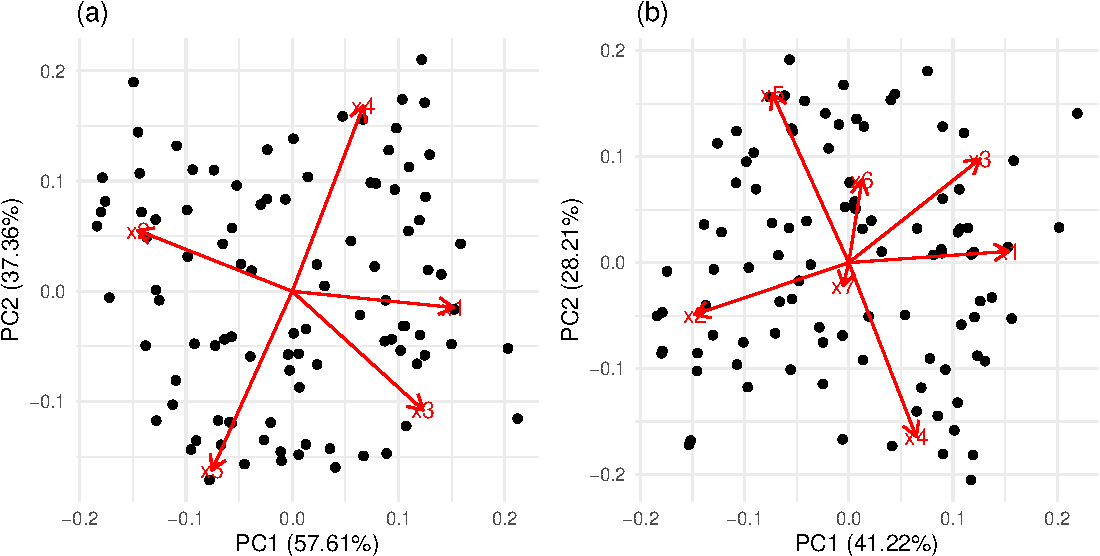
\includegraphics[width=0.8\textwidth,height=\textheight]{4-pca_files/figure-pdf/fig-plane-biplot-1.pdf}

}

\caption{\label{fig-plane-biplot}Biplots of the plane (a) and plane +
noise (b) data. All five variables contribute strongly to the two
principal components in (a): PC1 is primarily \texttt{x1}, \texttt{x2}
and \texttt{x3} and PC2 is primarily \texttt{x4} and \texttt{x5}. In (b)
the same four variables contribute in almost the same way, with
variables \texttt{x6} and \texttt{x7} contributing very little. The data
was constructed this way, that these two dimensions were purely noise.}

\end{figure}

It can be useful to examine this model using the tour. The model is
simply a plane in high dimensions. This would be considered to be the
model in the data space. The reason to do this is to check how well the
model fits the data. The plane corresponding to the model should be
oriented along the main direction of the points, and the spread of
points around the plane should be small. We should also be able to see
if there has been any strong non-linear relationship missed by the
model, or outliers and clusters.

The function \texttt{pca\_model()} from the \texttt{mulgar} package can
be used to represent the model as a \(k\)-D wire-frame plane.
\textbf{?@fig-plane-box-model} shows the models for the \texttt{plane}
and \texttt{box} data, 2D and 3D respectively.

\infobox{We look at the model in the data space to check how well the model fits the data. If it fits well, the points will cluster tightly around the model representation, with little spread in other directions.}

\begin{Shaded}
\begin{Highlighting}[]
\NormalTok{plane\_m }\OtherTok{\textless{}{-}} \FunctionTok{pca\_model}\NormalTok{(plane\_pca)}
\NormalTok{plane\_m\_d }\OtherTok{\textless{}{-}} \FunctionTok{rbind}\NormalTok{(plane\_m}\SpecialCharTok{$}\NormalTok{points, plane)}
\FunctionTok{animate\_xy}\NormalTok{(plane\_m\_d, }\AttributeTok{edges=}\NormalTok{plane\_m}\SpecialCharTok{$}\NormalTok{edges,}
           \AttributeTok{axes=}\StringTok{"bottomleft"}\NormalTok{,}
           \AttributeTok{edges.col=}\StringTok{"\#E7950F"}\NormalTok{,}
           \AttributeTok{edges.width=}\DecValTok{3}\NormalTok{)}
\FunctionTok{render\_gif}\NormalTok{(plane\_m\_d, }
           \FunctionTok{grand\_tour}\NormalTok{(), }
           \FunctionTok{display\_xy}\NormalTok{(}\AttributeTok{half\_range=}\FloatTok{0.9}\NormalTok{,}
                      \AttributeTok{edges=}\NormalTok{plane\_m}\SpecialCharTok{$}\NormalTok{edges, }
                      \AttributeTok{edges.col=}\StringTok{"\#E7950F"}\NormalTok{,}
                      \AttributeTok{edges.width=}\DecValTok{3}\NormalTok{),}
           \AttributeTok{gif\_file=}\StringTok{"gifs/plane\_model.gif"}\NormalTok{,}
           \AttributeTok{frames=}\DecValTok{500}\NormalTok{,}
           \AttributeTok{width=}\DecValTok{400}\NormalTok{,}
           \AttributeTok{height=}\DecValTok{400}\NormalTok{,}
           \AttributeTok{loop=}\ConstantTok{FALSE}\NormalTok{)}
\NormalTok{box\_pca }\OtherTok{\textless{}{-}} \FunctionTok{prcomp}\NormalTok{(box)}
\NormalTok{box\_m }\OtherTok{\textless{}{-}} \FunctionTok{pca\_model}\NormalTok{(box\_pca, }\AttributeTok{d=}\DecValTok{3}\NormalTok{)}
\NormalTok{box\_m\_d }\OtherTok{\textless{}{-}} \FunctionTok{rbind}\NormalTok{(box\_m}\SpecialCharTok{$}\NormalTok{points, box)}
\FunctionTok{animate\_xy}\NormalTok{(box\_m\_d, }\AttributeTok{edges=}\NormalTok{box\_m}\SpecialCharTok{$}\NormalTok{edges, }
           \AttributeTok{axes=}\StringTok{"bottomleft"}\NormalTok{, }\AttributeTok{edges.col=}\StringTok{"\#E7950F"}\NormalTok{, }\AttributeTok{edges.width=}\DecValTok{3}\NormalTok{)}
\FunctionTok{render\_gif}\NormalTok{(box\_m\_d, }
           \FunctionTok{grand\_tour}\NormalTok{(), }
           \FunctionTok{display\_xy}\NormalTok{(}\AttributeTok{half\_range=}\FloatTok{0.9}\NormalTok{,}
                      \AttributeTok{edges=}\NormalTok{box\_m}\SpecialCharTok{$}\NormalTok{edges, }
                      \AttributeTok{edges.col=}\StringTok{"\#E7950F"}\NormalTok{,}
                      \AttributeTok{edges.width=}\DecValTok{3}\NormalTok{),}
           \AttributeTok{gif\_file=}\StringTok{"gifs/box\_model.gif"}\NormalTok{,}
           \AttributeTok{frames=}\DecValTok{500}\NormalTok{,}
           \AttributeTok{width=}\DecValTok{400}\NormalTok{,}
           \AttributeTok{height=}\DecValTok{400}\NormalTok{,}
           \AttributeTok{loop=}\ConstantTok{FALSE}\NormalTok{)}
\end{Highlighting}
\end{Shaded}

\hypertarget{example-pisa-1}{%
\subsection{Example: pisa}\label{example-pisa-1}}

The model for the \texttt{pisa} data is a 1D vector, shown in
\textbf{?@fig-pisa-model}.

\begin{Shaded}
\begin{Highlighting}[]
\NormalTok{pisa\_model }\OtherTok{\textless{}{-}} \FunctionTok{pca\_model}\NormalTok{(pisa\_pca, }\AttributeTok{d=}\DecValTok{1}\NormalTok{, }\AttributeTok{s=}\DecValTok{2}\NormalTok{)}

\NormalTok{pisa\_all }\OtherTok{\textless{}{-}} \FunctionTok{rbind}\NormalTok{(pisa\_model}\SpecialCharTok{$}\NormalTok{points, pisa\_std)}
\FunctionTok{animate\_xy}\NormalTok{(pisa\_all, }\AttributeTok{edges=}\NormalTok{pisa\_model}\SpecialCharTok{$}\NormalTok{edges,}
           \AttributeTok{edges.col=}\StringTok{"\#E7950F"}\NormalTok{, }\AttributeTok{edges.width=}\DecValTok{3}\NormalTok{)}
\FunctionTok{render\_gif}\NormalTok{(pisa\_all, }
           \FunctionTok{grand\_tour}\NormalTok{(), }
           \FunctionTok{display\_xy}\NormalTok{(}\AttributeTok{half\_range=}\FloatTok{0.9}\NormalTok{,}
                      \AttributeTok{edges=}\NormalTok{pisa\_model}\SpecialCharTok{$}\NormalTok{edges, }
                      \AttributeTok{edges.col=}\StringTok{"\#E7950F"}\NormalTok{, }
                      \AttributeTok{edges.width=}\DecValTok{5}\NormalTok{),}
           \AttributeTok{gif\_file=}\StringTok{"gifs/pisa\_model.gif"}\NormalTok{,}
           \AttributeTok{frames=}\DecValTok{500}\NormalTok{,}
           \AttributeTok{width=}\DecValTok{400}\NormalTok{,}
           \AttributeTok{height=}\DecValTok{400}\NormalTok{,}
           \AttributeTok{loop=}\ConstantTok{FALSE}\NormalTok{)}
\end{Highlighting}
\end{Shaded}

\hypertarget{example-aflw-1}{%
\subsection{Example: aflw}\label{example-aflw-1}}

It is less useful to examine the PCA model for the \texttt{aflw} data,
because the main patterns that were of interest were the exceptional
players. However, we will do it anyway! \textbf{?@fig-aflw-model} shows
the 4D PCA model overlain on the data. Even though the distribution of
points is not as symmetric and balanced as the other examples, we can
see that the cube structure mirrors the variation. We can see that the
relationships between variables are not strictly linear, because the
spread extends unevenly away from the box.

\begin{Shaded}
\begin{Highlighting}[]
\NormalTok{aflw\_model }\OtherTok{\textless{}{-}} \FunctionTok{pca\_model}\NormalTok{(aflw\_pca, }\AttributeTok{d=}\DecValTok{4}\NormalTok{, }\AttributeTok{s=}\DecValTok{1}\NormalTok{)}

\NormalTok{aflw\_all }\OtherTok{\textless{}{-}} \FunctionTok{rbind}\NormalTok{(aflw\_model}\SpecialCharTok{$}\NormalTok{points, aflw\_std[,}\DecValTok{7}\SpecialCharTok{:}\DecValTok{35}\NormalTok{])}
\FunctionTok{animate\_xy}\NormalTok{(aflw\_all, }\AttributeTok{edges=}\NormalTok{aflw\_model}\SpecialCharTok{$}\NormalTok{edges,}
           \AttributeTok{edges.col=}\StringTok{"\#E7950F"}\NormalTok{, }
           \AttributeTok{edges.width=}\DecValTok{3}\NormalTok{, }
           \AttributeTok{half\_range=}\FloatTok{0.8}\NormalTok{, }
           \AttributeTok{axes=}\StringTok{"off"}\NormalTok{)}
\FunctionTok{render\_gif}\NormalTok{(aflw\_all, }
           \FunctionTok{grand\_tour}\NormalTok{(), }
           \FunctionTok{display\_xy}\NormalTok{(}\AttributeTok{half\_range=}\FloatTok{0.8}\NormalTok{,}
                      \AttributeTok{edges=}\NormalTok{aflw\_model}\SpecialCharTok{$}\NormalTok{edges, }
                      \AttributeTok{edges.col=}\StringTok{"\#E7950F"}\NormalTok{, }
                      \AttributeTok{edges.width=}\DecValTok{3}\NormalTok{, }
                      \AttributeTok{axes=}\StringTok{"off"}\NormalTok{),}
           \AttributeTok{gif\_file=}\StringTok{"gifs/aflw\_model.gif"}\NormalTok{,}
           \AttributeTok{frames=}\DecValTok{500}\NormalTok{,}
           \AttributeTok{width=}\DecValTok{400}\NormalTok{,}
           \AttributeTok{height=}\DecValTok{400}\NormalTok{,}
           \AttributeTok{loop=}\ConstantTok{FALSE}\NormalTok{)}
\end{Highlighting}
\end{Shaded}

\hypertarget{when-relationships-are-not-linear}{%
\section{When relationships are not
linear}\label{when-relationships-are-not-linear}}

\hypertarget{example-outliers}{%
\subsection{Example: outliers}\label{example-outliers}}

Figure~\ref{fig-plane-n-o-scree} shows the scree plot for the planar
data with noise and outliers. It is very similar to the scree plot on
the data without the outliers (Figure~\ref{fig-plane-noise-scree}).
However, what we see from \textbf{?@fig-p-o-pca} is that PCA loses the
outliers. The animation in (a) shows the full data, and the outliers
marked by colour and labels 1, 2, are clearly unusual in some
projections. When we examine the tour of the first four PCs (as
suggested by the scree plot) the outliers are not unusual. They are
almost contained in the point cloud. The reason is clear when all the
PCs are plotted, and the outliers can be seen to be clearly detected
only in PC5, PC6 and PC7.

\begin{Shaded}
\begin{Highlighting}[]
\NormalTok{plane\_n\_o\_pca }\OtherTok{\textless{}{-}} \FunctionTok{prcomp}\NormalTok{(plane\_noise\_outliers)}
\FunctionTok{ggscree}\NormalTok{(plane\_n\_o\_pca, }\AttributeTok{q =} \DecValTok{7}\NormalTok{) }\SpecialCharTok{+} \FunctionTok{theme\_minimal}\NormalTok{()}
\end{Highlighting}
\end{Shaded}

\begin{figure}[H]

{\centering 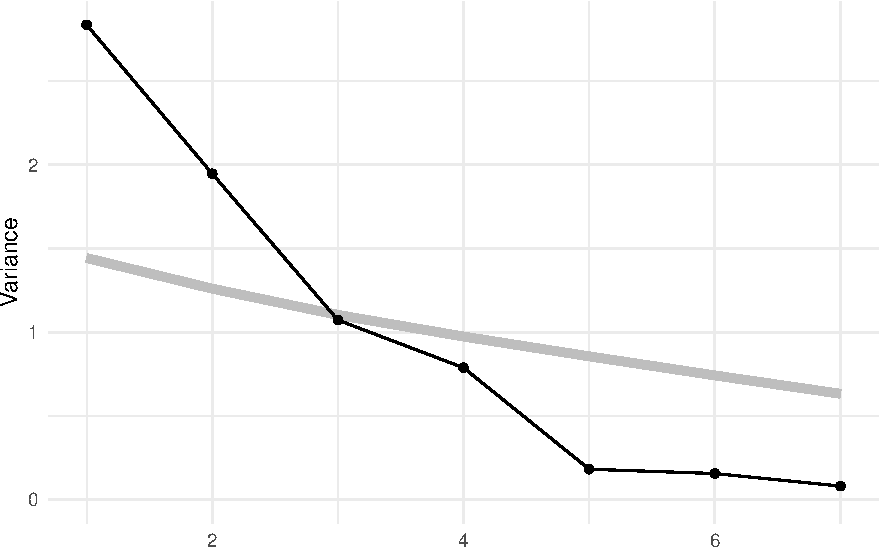
\includegraphics[width=0.8\textwidth,height=\textheight]{4-pca_files/figure-pdf/fig-plane-n-o-scree-1.pdf}

}

\caption{\label{fig-plane-n-o-scree}Scree plot of the planar data with
noise and an outlier. It is almost the same as the data without the
outliers.}

\end{figure}

\begin{Shaded}
\begin{Highlighting}[]
\NormalTok{clrs }\OtherTok{\textless{}{-}} \FunctionTok{hcl.colors}\NormalTok{(}\DecValTok{12}\NormalTok{, }\StringTok{"Zissou 1"}\NormalTok{)}
\NormalTok{p\_col }\OtherTok{\textless{}{-}} \FunctionTok{c}\NormalTok{(}\FunctionTok{rep}\NormalTok{(}\StringTok{"black"}\NormalTok{, }\DecValTok{100}\NormalTok{), clrs[}\DecValTok{11}\NormalTok{], clrs[}\DecValTok{11}\NormalTok{])}
\NormalTok{p\_obs\_labels }\OtherTok{\textless{}{-}} \FunctionTok{c}\NormalTok{(}\FunctionTok{rep}\NormalTok{(}\StringTok{""}\NormalTok{, }\DecValTok{100}\NormalTok{), }\StringTok{"1"}\NormalTok{, }\StringTok{"2"}\NormalTok{)}

\FunctionTok{animate\_xy}\NormalTok{(plane\_n\_o\_pca}\SpecialCharTok{$}\NormalTok{x[,}\DecValTok{1}\SpecialCharTok{:}\DecValTok{4}\NormalTok{],}
           \AttributeTok{col=}\NormalTok{p\_col,}
           \AttributeTok{obs\_labels=}\NormalTok{p\_obs\_labels)}
\FunctionTok{animate\_xy}\NormalTok{(plane\_noise\_outliers,}
           \AttributeTok{col=}\NormalTok{p\_col,}
           \AttributeTok{obs\_labels=}\NormalTok{p\_obs\_labels)}
\FunctionTok{render\_gif}\NormalTok{(plane\_noise\_outliers, }
           \FunctionTok{grand\_tour}\NormalTok{(), }
           \FunctionTok{display\_xy}\NormalTok{(}\AttributeTok{half\_range=}\FloatTok{0.8}\NormalTok{,}
                      \AttributeTok{col=}\NormalTok{p\_col,}
             \AttributeTok{obs\_labels=}\NormalTok{p\_obs\_labels),}
           \AttributeTok{gif\_file=}\StringTok{"gifs/plane\_n\_o\_clr.gif"}\NormalTok{,}
           \AttributeTok{frames=}\DecValTok{500}\NormalTok{,}
           \AttributeTok{width=}\DecValTok{200}\NormalTok{,}
           \AttributeTok{height=}\DecValTok{200}\NormalTok{,}
           \AttributeTok{loop=}\ConstantTok{FALSE}\NormalTok{)}
\FunctionTok{render\_gif}\NormalTok{(plane\_n\_o\_pca}\SpecialCharTok{$}\NormalTok{x[,}\DecValTok{1}\SpecialCharTok{:}\DecValTok{4}\NormalTok{], }
           \FunctionTok{grand\_tour}\NormalTok{(), }
           \FunctionTok{display\_xy}\NormalTok{(}\AttributeTok{half\_range=}\FloatTok{0.8}\NormalTok{,}
                      \AttributeTok{col=}\NormalTok{p\_col,}
             \AttributeTok{obs\_labels=}\NormalTok{p\_obs\_labels),}
           \AttributeTok{gif\_file=}\StringTok{"gifs/plane\_n\_o\_pca.gif"}\NormalTok{,}
           \AttributeTok{frames=}\DecValTok{500}\NormalTok{,}
           \AttributeTok{width=}\DecValTok{200}\NormalTok{,}
           \AttributeTok{height=}\DecValTok{200}\NormalTok{,}
           \AttributeTok{loop=}\ConstantTok{FALSE}\NormalTok{)}
\end{Highlighting}
\end{Shaded}

\begin{Shaded}
\begin{Highlighting}[]
\FunctionTok{library}\NormalTok{(GGally)}
\FunctionTok{ggscatmat}\NormalTok{(plane\_n\_o\_pca}\SpecialCharTok{$}\NormalTok{x) }\SpecialCharTok{+} \FunctionTok{theme\_minimal}\NormalTok{()}
\end{Highlighting}
\end{Shaded}

\begin{figure}[H]

{\centering 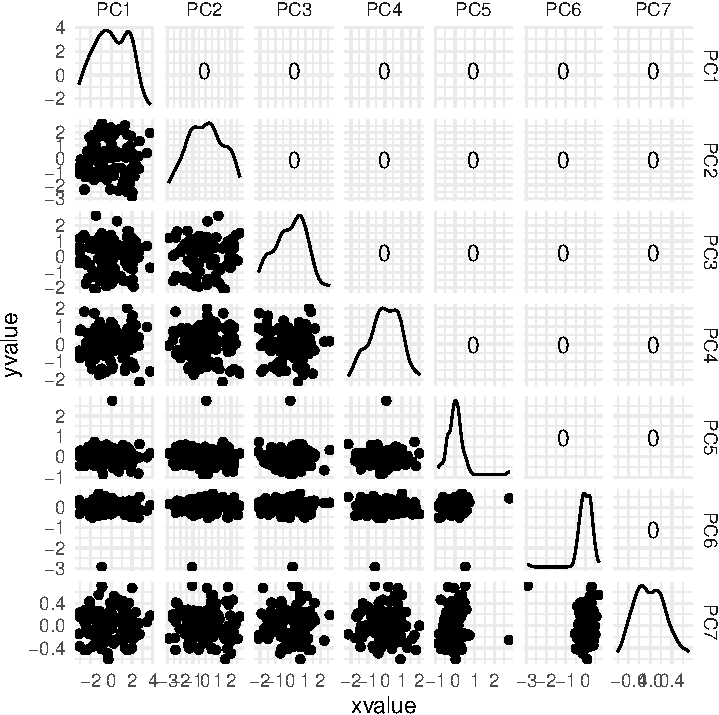
\includegraphics[width=0.8\textwidth,height=\textheight]{4-pca_files/figure-pdf/fig-plane-o-n-pairs-1.pdf}

}

\caption{\label{fig-plane-o-n-pairs}From the scatterplot matrix we can
see that the outliers are present in PC5, PC6 and PC7. That means by
reducing the dimensionality to the first four PCs the model has missed
some important characteristics in the data.}

\end{figure}

\hypertarget{example-non-linear-associations}{%
\subsection{Example: Non-linear
associations}\label{example-non-linear-associations}}

\textbf{?@fig-plane-nonlin} shows the tour of the full 5D data
containing non-linear relationships in comparison with a tour of the
first three PCs, as recommended by the scree plot
(Figure~\ref{fig-plane-nonlin-scree}). The PCs capture some clear and
very clean non-linear relationship, but it looks like it has missed some
of the complexities of the relationships. The scatterplot matrix of all
5 PCs (Figure~\ref{fig-plane-nonlin-pairs}) shows that PC4 and PC5
contain interesting features: more non-linearity, and curiously an
outlier.

\begin{Shaded}
\begin{Highlighting}[]
\FunctionTok{data}\NormalTok{(plane\_nonlin)}
\NormalTok{plane\_nonlin\_pca }\OtherTok{\textless{}{-}} \FunctionTok{prcomp}\NormalTok{(plane\_nonlin)}
\FunctionTok{ggscree}\NormalTok{(plane\_nonlin\_pca, }\AttributeTok{q =} \DecValTok{5}\NormalTok{) }\SpecialCharTok{+} \FunctionTok{theme\_minimal}\NormalTok{()}
\end{Highlighting}
\end{Shaded}

\begin{figure}[H]

{\centering 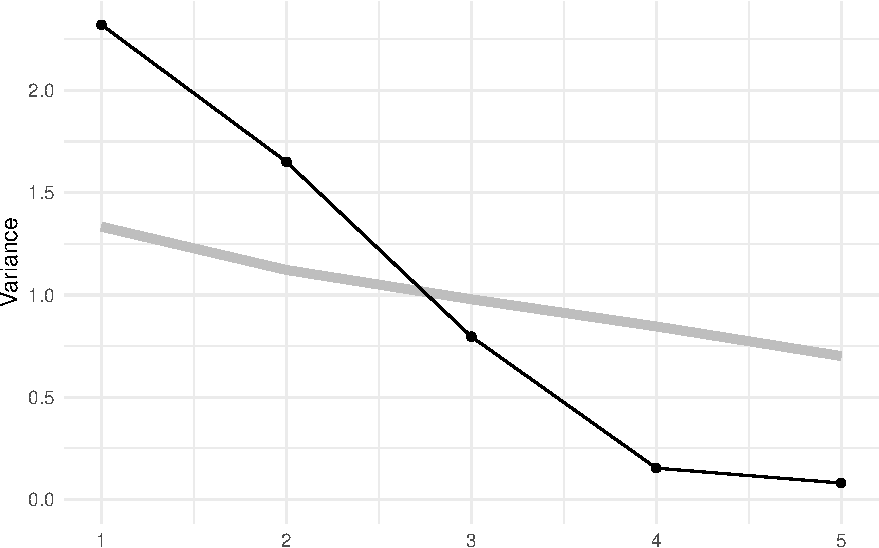
\includegraphics[width=0.8\textwidth,height=\textheight]{4-pca_files/figure-pdf/fig-plane-nonlin-scree-1.pdf}

}

\caption{\label{fig-plane-nonlin-scree}Scree plot of the non-linear data
suggests three PCs.}

\end{figure}

\begin{Shaded}
\begin{Highlighting}[]
\FunctionTok{animate\_xy}\NormalTok{(plane\_nonlin\_pca}\SpecialCharTok{$}\NormalTok{x[,}\DecValTok{1}\SpecialCharTok{:}\DecValTok{3}\NormalTok{])}
\FunctionTok{render\_gif}\NormalTok{(plane\_nonlin\_pca}\SpecialCharTok{$}\NormalTok{x[,}\DecValTok{1}\SpecialCharTok{:}\DecValTok{3}\NormalTok{], }
           \FunctionTok{grand\_tour}\NormalTok{(), }
           \FunctionTok{display\_xy}\NormalTok{(}\AttributeTok{half\_range=}\FloatTok{0.8}\NormalTok{),}
           \AttributeTok{gif\_file=}\StringTok{"gifs/plane\_nonlin\_pca.gif"}\NormalTok{,}
           \AttributeTok{frames=}\DecValTok{500}\NormalTok{,}
           \AttributeTok{width=}\DecValTok{200}\NormalTok{,}
           \AttributeTok{height=}\DecValTok{200}\NormalTok{)}
\end{Highlighting}
\end{Shaded}

\begin{Shaded}
\begin{Highlighting}[]
\FunctionTok{ggscatmat}\NormalTok{(plane\_nonlin\_pca}\SpecialCharTok{$}\NormalTok{x)}
\end{Highlighting}
\end{Shaded}

\begin{figure}[H]

{\centering 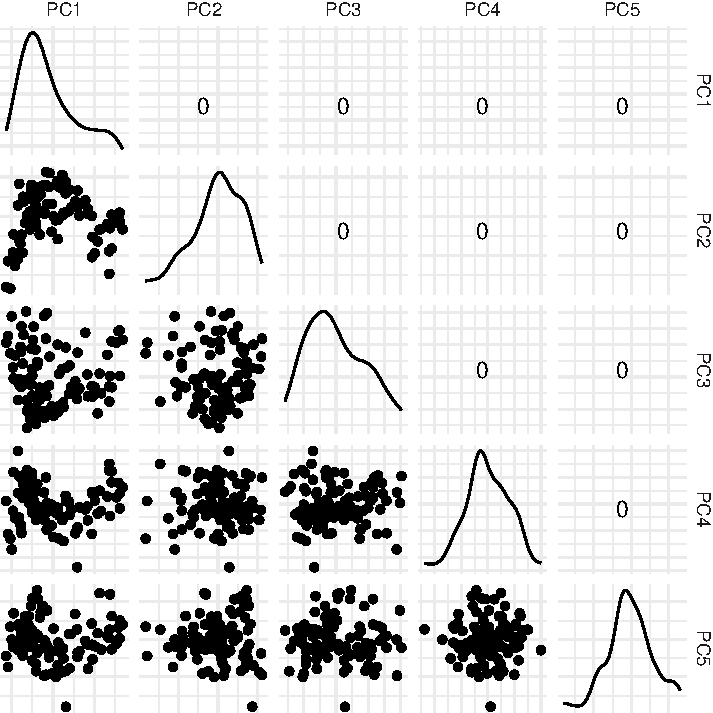
\includegraphics[width=0.8\textwidth,height=\textheight]{4-pca_files/figure-pdf/fig-plane-nonlin-pairs-1.pdf}

}

\caption{\label{fig-plane-nonlin-pairs}From the scatterplot matrix we
can see that the there is a non-linear relationship visible in PC1 and
PC2, with perhaps a small contribution from PC3. However, we can see
that when the data is reduced to three PCs, it misses catching all on
the non-linear relationships and also interestingly it seems that there
is an unusual observation also.}

\end{figure}

\infobox{One of the dangers of PCA is that interesting and curious details of the data only emerge in the lowest PCs, that are usually discarded. The tour, and examining the smaller PCs, can help to discover them.}

\hypertarget{exercises-3}{%
\section*{Exercises}\label{exercises-3}}
\addcontentsline{toc}{section}{Exercises}

\markright{Exercises}

\begin{enumerate}
\def\labelenumi{\arabic{enumi}.}
\tightlist
\item
  Make a scatterplot matrix of the first four PCs of the \texttt{aflw}
  data. Is the branch pattern visible in any pair?
\item
  Construct five new variables to measure these skills offense, defense,
  playing time, ball movement, errors. Using the tour, examine the
  relationship between these variables. Map out how a few players could
  be characterised based on these directions of skills.
\item
  Symmetrise any \texttt{aflw} variables that have skewed distributions
  using a log or square root transformation. Then re-do the PCA. What do
  we learn that is different about associations between the skill
  variables?
\item
  Examine the \texttt{bushfires} data using a grand tour on the numeric
  variables, ignoring the \texttt{cause} (class) variable. Note any
  issues such as outliers, or skewness that might affect PCA. How many
  principal components would be recommended by the scree plot? Examine
  this PCA model with the data, and explain how well it does or doesn't
  fit.
\item
  Use the \texttt{pca\_tour} to examine the first five PCs of the
  \texttt{bushfires} data. How do all of the variables contribute to
  this reduced space?
\item
  Reduce the dimension of the \texttt{sketches} data to 12 PCs. How much
  variation does this explain? Is there any obvious clustering in this
  lower dimensional space?
\end{enumerate}

\hypertarget{project}{%
\section*{Project}\label{project}}
\addcontentsline{toc}{section}{Project}

\markright{Project}

Linear dimension reduction can optimise for other criteria, and here we
will explore one example: the algorithm implemented in the
\texttt{dobin} package finds a basis in which the first few directions
are optimized for the detection of outliers in the data. We will examine
how it performs for the \texttt{plane\_noise\_outliers} data (the
example where outliers were hidden in the first four principal
components.)

\begin{enumerate}
\def\labelenumi{\arabic{enumi}.}
\tightlist
\item
  Start by looking up the documentation of \texttt{dobin::dobin}. How
  many parameters does the method depend on?
\item
  We first apply the function to the \texttt{plane\_noise\_outliers}
  data using default values for all parameters.
\item
  Recall that the outliers were added in rows 101 and 102 of the data.
  Make a scatter plots showing the projection onto the first, second and
  third component, using color to highlight the outliers. Are they
  visible as outliers with three components?
\item
  Adjust the \texttt{frac} parameter of the \texttt{dobin} function to
  \texttt{frac\ =\ 0.99} and repeat the graphical evaluation from point
  3. How does it compare to the previous solution?
\end{enumerate}

\hypertarget{non-linear-dimension-reduction}{%
\chapter{Non-linear dimension
reduction}\label{non-linear-dimension-reduction}}

\hypertarget{background}{%
\section{Background}\label{background}}

Non-linear dimension reduction (NLDR) aims to find a low-dimensional
representation of the high-dimensional data that shows the main features
of the data. In statistics, it dates back to Kruskal (1964a)'s work on
multidimensional scaling (MDS). Some techniques only require an
interpoint similarity or distance matrix as the main ingredient, rather
than the full data. We'll focus on when the full data is available here,
so we can also compare structure perceived using the tour on the
high-dimensional space, relative to structure revealed in the
low-dimensional embedding.

There are many methods available for generating non-linear low
dimensional representations of the data. MDS is a classical technique
that minimises the difference between two interpoint distance matrices,
the distance between points in the high-dimensions, and in the
low-dimensional representations. A good resource for learning about MDS
is Borg \& Groenen (2005).

\begin{Shaded}
\begin{Highlighting}[]
\FunctionTok{library}\NormalTok{(mulgar)}
\FunctionTok{library}\NormalTok{(Rtsne)}
\FunctionTok{library}\NormalTok{(uwot)}
\FunctionTok{library}\NormalTok{(ggplot2)}
\FunctionTok{library}\NormalTok{(patchwork)}
\FunctionTok{set.seed}\NormalTok{(}\DecValTok{42}\NormalTok{)}
\NormalTok{cnl\_tsne }\OtherTok{\textless{}{-}} \FunctionTok{Rtsne}\NormalTok{(clusters\_nonlin)}
\NormalTok{cnl\_umap }\OtherTok{\textless{}{-}} \FunctionTok{umap}\NormalTok{(clusters\_nonlin)}
\NormalTok{n1 }\OtherTok{\textless{}{-}} \FunctionTok{ggplot}\NormalTok{(}\FunctionTok{as.data.frame}\NormalTok{(cnl\_tsne}\SpecialCharTok{$}\NormalTok{Y), }\FunctionTok{aes}\NormalTok{(}\AttributeTok{x=}\NormalTok{V1, }\AttributeTok{y=}\NormalTok{V2)) }\SpecialCharTok{+}
  \FunctionTok{geom\_point}\NormalTok{() }\SpecialCharTok{+} 
  \FunctionTok{ggtitle}\NormalTok{(}\StringTok{"(a) t{-}SNE"}\NormalTok{) }\SpecialCharTok{+}
  \FunctionTok{theme\_minimal}\NormalTok{() }\SpecialCharTok{+} 
  \FunctionTok{theme}\NormalTok{(}\AttributeTok{aspect.ratio=}\DecValTok{1}\NormalTok{)}
\NormalTok{n2 }\OtherTok{\textless{}{-}} \FunctionTok{ggplot}\NormalTok{(}\FunctionTok{as.data.frame}\NormalTok{(cnl\_umap), }\FunctionTok{aes}\NormalTok{(}\AttributeTok{x=}\NormalTok{V1, }\AttributeTok{y=}\NormalTok{V2)) }\SpecialCharTok{+}
  \FunctionTok{geom\_point}\NormalTok{() }\SpecialCharTok{+} 
  \FunctionTok{ggtitle}\NormalTok{(}\StringTok{"(b) UMAP"}\NormalTok{) }\SpecialCharTok{+}
  \FunctionTok{theme\_minimal}\NormalTok{() }\SpecialCharTok{+} 
  \FunctionTok{theme}\NormalTok{(}\AttributeTok{aspect.ratio=}\DecValTok{1}\NormalTok{)}
\NormalTok{n1 }\SpecialCharTok{+}\NormalTok{ n2}
\end{Highlighting}
\end{Shaded}

\begin{figure}[H]

{\centering 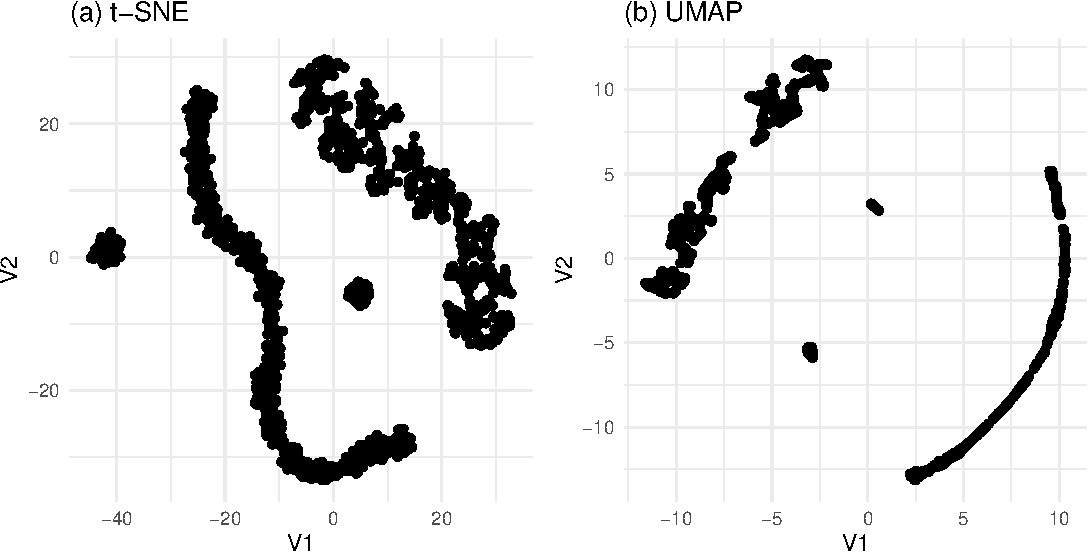
\includegraphics[width=0.8\textwidth,height=\textheight]{5-nldr_files/figure-pdf/fig-nldr-clusters-1.pdf}

}

\caption{\label{fig-nldr-clusters}Two non-linear embeddings of the
non-linear clusters data: (a) t-SNE, (b) UMAP. Both suggest four
clusters, with two being non-linear in some form.}

\end{figure}

Figure~\ref{fig-nldr-clusters} show two NLDR views of the
\texttt{clusters\_nonlin} data set from the \texttt{mulgar} package.
Both suggest that there are four clusters, and that some clusters are
non-linearly shaped. They disagree on the type of non-linear pattern,
where t-SNE represents one cluster as a wavy-shape and UMAP both have a
simple parabolic shape. Popular methods in current use include t-SNE
(Maaten \& Hinton, 2008), UMAP (McInnes et al., 2018) and PHATE (Moon et
al., 2019).

\begin{Shaded}
\begin{Highlighting}[]
\FunctionTok{library}\NormalTok{(tourr)}
\FunctionTok{render\_gif}\NormalTok{(clusters\_nonlin, }
           \FunctionTok{grand\_tour}\NormalTok{(),}
           \FunctionTok{display\_xy}\NormalTok{(),}
           \AttributeTok{gif\_file =} \StringTok{"gifs/clusters\_nonlin.gif"}\NormalTok{,}
           \AttributeTok{frames =} \DecValTok{500}\NormalTok{,}
           \AttributeTok{width =} \DecValTok{300}\NormalTok{, }
           \AttributeTok{height =} \DecValTok{300}\NormalTok{)}
\end{Highlighting}
\end{Shaded}

The full 4D data is shown with a grand tour in
\textbf{?@fig-clusters-nonlin}. The four clusters suggested by the NLDR
methods can be seen. We also get a better sense of the relative size and
proximity of the clusters. There are two small spherical clusters, one
quite close to the end of the large sine wave cluster. The fourth
cluster is relatively small, and has a slight curve, like a bent rod.
The t-SNE representation is slightly more accurate than the UMAP
representation. We would expect that the wavy cluster is the sine wave
seen in the tour.

NLDR can provide useful low-dimensional summaries of high-dimensional
structure but you need to check whether it is a sensible and accurate
representation by comparing with what is perceivd from a tour.

\hypertarget{linking-nldr-representation-with-tour-view}{%
\section{Linking NLDR representation with tour
view}\label{linking-nldr-representation-with-tour-view}}

NLDR can produce useful low-dimensional summaries of structure in
high-dimensional data, like those shown in
Figure~\ref{fig-nldr-clusters}. However, there are numerous pitfalls.
The fitting procedure can produce very different representations
depending on the parameter choices, and even the random number seeding
the fit. (You can check this by changing the \texttt{set.seed} in the
code above, and by changing from the default parameters.) Also, it may
not be possible to represent the high-dimensional structures faithfully
low dimensions. For these reasons, one needs to connect the NLDR view
with a tour of the data, to help assess its usefulness and accuracy. For
example, with this data, we would want to know which of the two curved
clusters in the UMAP representation correspond to the sine wave cluster.

\hypertarget{using-liminal}{%
\subsection{\texorpdfstring{Using
\texttt{liminal}}{Using liminal}}\label{using-liminal}}

Figure~\ref{fig-liminal-clusters-nonlin} shows how the NLDR plot can be
linked to a tour view, using the \texttt{liminal} package, to better
understand how well the structure of the data is represented. Here we
see learn that the smile in the UMAP embedding is the small bent rod
cluster, and that the unibrow is the sine wave.

\begin{Shaded}
\begin{Highlighting}[]
\FunctionTok{library}\NormalTok{(liminal)}
\NormalTok{umap\_df }\OtherTok{\textless{}{-}} \FunctionTok{data.frame}\NormalTok{(}\AttributeTok{umapX =}\NormalTok{ cnl\_umap[, }\DecValTok{1}\NormalTok{],}
                      \AttributeTok{umapY =}\NormalTok{ cnl\_umap[, }\DecValTok{2}\NormalTok{])}
\FunctionTok{limn\_tour\_link}\NormalTok{(}
\NormalTok{  umap\_df,}
\NormalTok{  clusters\_nonlin,}
  \AttributeTok{cols =}\NormalTok{ x1}\SpecialCharTok{:}\NormalTok{x4}
\NormalTok{)}
\end{Highlighting}
\end{Shaded}

\begin{figure}

{\centering 

}

\caption{\label{fig-liminal-clusters-nonlin}Two screenshots from liminal
showing which clusters match between the UMAP representation and the
tour animation. The smile corresponds to the small bent rod cluster. The
unibrow matches to the sine wave cluster.}

\end{figure}

\hypertarget{using-detourr}{%
\subsection{\texorpdfstring{Using
\texttt{detourr}}{Using detourr}}\label{using-detourr}}

\textbf{?@fig-detourr-clusters-nonlin} shows how the linking is achieved
using \texttt{detourr}. It uses a shared data object, as made possible
by the \texttt{crosstalk} package, and the UMAP view is made interactive
using \texttt{plotly}.

\begin{Shaded}
\begin{Highlighting}[]
\FunctionTok{library}\NormalTok{(detourr)}
\FunctionTok{library}\NormalTok{(dplyr)}
\FunctionTok{library}\NormalTok{(crosstalk)}
\FunctionTok{library}\NormalTok{(plotly)}
\NormalTok{umap\_df }\OtherTok{\textless{}{-}} \FunctionTok{data.frame}\NormalTok{(}\AttributeTok{umapX =}\NormalTok{ cnl\_umap[, }\DecValTok{1}\NormalTok{],}
                      \AttributeTok{umapY =}\NormalTok{ cnl\_umap[, }\DecValTok{2}\NormalTok{])}
\NormalTok{cnl\_df }\OtherTok{\textless{}{-}} \FunctionTok{bind\_cols}\NormalTok{(clusters\_nonlin, umap\_df)}
\NormalTok{shared\_cnl }\OtherTok{\textless{}{-}}\NormalTok{ SharedData}\SpecialCharTok{$}\FunctionTok{new}\NormalTok{(cnl\_df)}

\NormalTok{detour\_plot }\OtherTok{\textless{}{-}} \FunctionTok{detour}\NormalTok{(shared\_cnl, }\FunctionTok{tour\_aes}\NormalTok{(}
  \AttributeTok{projection =} \FunctionTok{starts\_with}\NormalTok{(}\StringTok{"x"}\NormalTok{))) }\SpecialCharTok{|\textgreater{}}
    \FunctionTok{tour\_path}\NormalTok{(}\FunctionTok{grand\_tour}\NormalTok{(}\DecValTok{2}\NormalTok{), }
                    \AttributeTok{max\_bases=}\DecValTok{50}\NormalTok{, }\AttributeTok{fps =} \DecValTok{60}\NormalTok{) }\SpecialCharTok{|\textgreater{}}
       \FunctionTok{show\_scatter}\NormalTok{(}\AttributeTok{alpha =} \FloatTok{0.7}\NormalTok{, }\AttributeTok{axes =} \ConstantTok{FALSE}\NormalTok{,}
                    \AttributeTok{width =} \StringTok{"100\%"}\NormalTok{, }\AttributeTok{height =} \StringTok{"450px"}\NormalTok{)}

\NormalTok{umap\_plot }\OtherTok{\textless{}{-}} \FunctionTok{plot\_ly}\NormalTok{(shared\_cnl,}
                    \AttributeTok{x =} \SpecialCharTok{\textasciitilde{}}\NormalTok{umapX, }
                    \AttributeTok{y =} \SpecialCharTok{\textasciitilde{}}\NormalTok{umapY,}
                    \AttributeTok{color =} \FunctionTok{I}\NormalTok{(}\StringTok{"black"}\NormalTok{),}
                    \AttributeTok{height =} \DecValTok{450}\NormalTok{) }\SpecialCharTok{\%\textgreater{}\%}
    \FunctionTok{highlight}\NormalTok{(}\AttributeTok{on =} \StringTok{"plotly\_selected"}\NormalTok{, }
              \AttributeTok{off =} \StringTok{"plotly\_doubleclick"}\NormalTok{) }\SpecialCharTok{\%\textgreater{}\%}
    \FunctionTok{add\_trace}\NormalTok{(}\AttributeTok{type =} \StringTok{"scatter"}\NormalTok{, }
              \AttributeTok{mode =} \StringTok{"markers"}\NormalTok{)}

\FunctionTok{bscols}\NormalTok{(}
\NormalTok{     detour\_plot, umap\_plot,}
     \AttributeTok{widths =} \FunctionTok{c}\NormalTok{(}\DecValTok{5}\NormalTok{, }\DecValTok{6}\NormalTok{)}
\NormalTok{ )}
\end{Highlighting}
\end{Shaded}

\hypertarget{example-fake_trees}{%
\section{\texorpdfstring{Example:
\texttt{fake\_trees}}{Example: fake\_trees}}\label{example-fake_trees}}

Figure~\ref{fig-liminal-trees} shows a more complex example, using the
\texttt{fake\_trees} data. We know that the 10D data has a main branch,
and 9 branches (clusters) attached to it, absed on our explorations in
the earlier chapters. The t-SNE view, where points are coloured by the
known branch ids, is very helpful for seeing the linear branch
structure.

What we can't tell is that there is a main branch from which all of the
others extend. We also can't tell which of the clusters corresponds to
this branch. Linking the plot with a tour helps with this. Although, not
shown in the sequence of snapshots in Figure~\ref{fig-liminal-trees},
the main branch is actually the dark blue cluster, which is separated
into three pieces by t-SNE.

\begin{Shaded}
\begin{Highlighting}[]
\FunctionTok{library}\NormalTok{(liminal)}
\FunctionTok{library}\NormalTok{(Rtsne)}
\FunctionTok{data}\NormalTok{(fake\_trees)}
\FunctionTok{set.seed}\NormalTok{(}\DecValTok{2020}\NormalTok{)}
\NormalTok{tsne }\OtherTok{\textless{}{-}}\NormalTok{ Rtsne}\SpecialCharTok{::}\FunctionTok{Rtsne}\NormalTok{(dplyr}\SpecialCharTok{::}\FunctionTok{select}\NormalTok{(fake\_trees, dplyr}\SpecialCharTok{::}\FunctionTok{starts\_with}\NormalTok{(}\StringTok{"dim"}\NormalTok{)))}
\NormalTok{tsne\_df }\OtherTok{\textless{}{-}} \FunctionTok{data.frame}\NormalTok{(}\AttributeTok{tsneX =}\NormalTok{ tsne}\SpecialCharTok{$}\NormalTok{Y[, }\DecValTok{1}\NormalTok{],}
                      \AttributeTok{tsneY =}\NormalTok{ tsne}\SpecialCharTok{$}\NormalTok{Y[, }\DecValTok{2}\NormalTok{])}
\FunctionTok{limn\_tour\_link}\NormalTok{(}
\NormalTok{  tsne\_df,}
\NormalTok{  fake\_trees,}
  \AttributeTok{cols =}\NormalTok{ dim1}\SpecialCharTok{:}\NormalTok{dim10,}
  \AttributeTok{color =}\NormalTok{ branches}
\NormalTok{)}
\end{Highlighting}
\end{Shaded}

\begin{figure}

{\centering 

}

\caption{\label{fig-liminal-trees}Three snapshots of using the
\texttt{liminal} linked views to explore how t-SNE has summarised the
\texttt{fake\_trees} data in 2D.}

\end{figure}

The t-SNE representation clearly shows the linear structures of the
data, but viewing this 10D data with the tour shows that t-SNE makes
several inaccurate breaks of some of the branches.

\hypertarget{exercises-4}{%
\section*{Exercises}\label{exercises-4}}
\addcontentsline{toc}{section}{Exercises}

\markright{Exercises}

\begin{enumerate}
\def\labelenumi{\arabic{enumi}.}
\tightlist
\item
  Using the \texttt{penguins\_sub} data generate a 2D representation
  using t-SNE. Plot the points mapping the colour to species. What is
  most surprising? (Hint: Are the three species represented by three
  distinct clusters?)
\item
  Re-do the t-SNE representation with different parameter choices. Are
  the results different each time, or could they be considered to be
  equivalent?
\item
  Use \texttt{liminal} to link the t-SNE representation to a tour of the
  penguins. Highlight the points that have been placed in an awkward
  position by t-SNE from others in their species. Watch them relative to
  the others in their species in the tour view, and think about whether
  there is any rationale for the awkward placement.
\item
  Use UMAP to make the 2D representation, and use \texttt{liminal} to
  link with a tour to explore the result.
\item
  Repeat 1-4 using \texttt{detourr}.
\end{enumerate}

\part{Cluster analysis}

\hypertarget{overview}{%
\chapter{Overview}\label{overview}}

Unsupervised classification, or cluster analysis, organizes observations
into similar groups. Cluster analysis is a commonly used, appealing, and
conceptually intuitive statistical method. Some of its uses include
market segmentation, where customers are grouped into clusters with
similar attributes for targeted marketing; gene expression analysis,
where genes with similar expression patterns are grouped together; and
the creation of taxonomies for animals, insects, or plants. Clustering
can be used as a way of reducing a massive amount of data because
observations within a cluster can be summarized by its centre. Also,
clustering effectively subsets the data thus simplifying analysis
because observations in each cluster can be analyzed separately.

\hypertarget{what-are-clusters}{%
\section{What are clusters?}\label{what-are-clusters}}

Organizing objects into groups is a common task to help make sense of
the world around us. Perhaps this is why it is an appealing method of
data analysis. However, cluster analysis is more complex than it
initially appears. Many people imagine that it will produce neatly
separated clusters like those in Figure~\ref{fig-ideal-clusters}(a), but
it almost never does. Such ideal clusters are rarely encountered in real
data, so we often need to modify our objective from \emph{find the
natural clusters in this data}. Instead, we need to organize the
\emph{cases into groups that are similar in some way}. Even though this
may seem disappointing when compared with the ideal, it is still often
an effective means of simplifying and understanding a dataset.

Knowing what shapes are in your data helps to decide on the best method
and to diagnose the result. For example, if the clusters are elliptical
model-based clustering is recommended.

\begin{figure}

{\centering 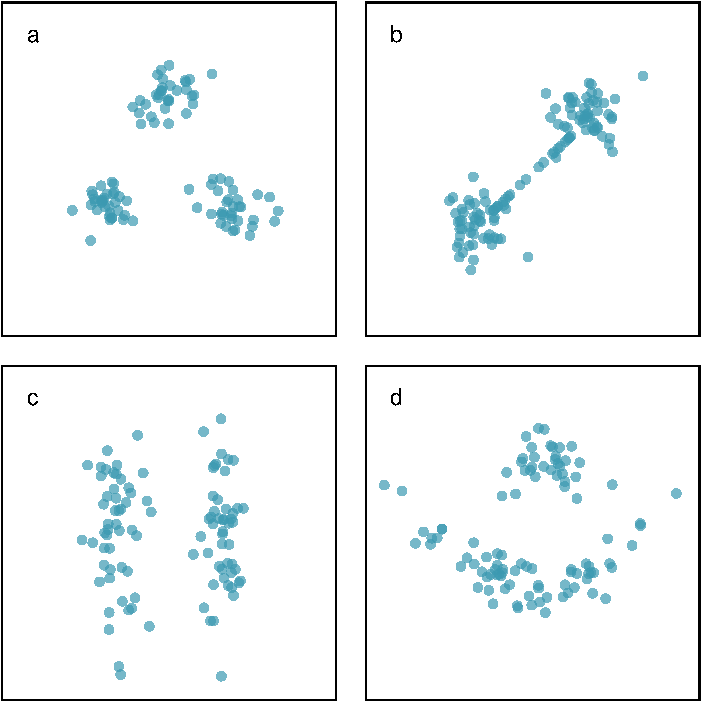
\includegraphics[width=1\textwidth,height=\textheight]{6-intro-clust_files/figure-pdf/fig-ideal-clusters-1.pdf}

}

\caption{\label{fig-ideal-clusters}Different structures in data impact
cluster analysis. When there are well-separated groups (a), it is simple
to group similar observations. Even when there are not, partitioning
observations into groups may still be useful. There may be nuisance
observations (b) or nuisance variables (c) that affect the interpoint
distance calculations and distract the clustering algorithm, and there
may oddly shaped clusters (d) which are hard to numerically describe.}

\end{figure}

At the heart of the clustering process is the work of discovering which
variables are most important for defining the groups. It is often true
that we only require a subset of the variables for finding clusters,
whereas another subset (called \emph{nuisance variables}) has no impact.
In the bottom left plot of Figure~\ref{fig-ideal-clusters}, it is clear
that the variable plotted horizontally is important for splitting this
data into two clusters, whereas the variable plotted vertically is a
nuisance variable. Nuisance is an apt term for these variables, because
they can radically change the interpoint distances and impair the
clustering process. \index{cluster analysis!interpoint distance}
\index{cluster analysis!nuisance variable}

Dynamic graphical methods help us to find and understand the cluster
structure in high dimensions. With the tools in our toolbox, primarily
tours, along with linked scatterplots and parallel coordinate plots, we
can see clusters in high-dimensional spaces. We can detect gaps between
clusters, the shape and relative positions of clusters, and the presence
of nuisance variables. We can even find unusually shaped clusters, like
those in the bottom right plot in Figure~\ref{fig-ideal-clusters}. In
simple situations we can use graphics alone to group observations into
clusters, using a ``spin and brush'' method. In more difficult data
problems, we can assess and refine numerical solutions using
graphics.\index{brushing!persistent}
\index{cluster analysis!spin and brush}

This part of the book discusses the use of interactive and dynamic
graphics in the clustering of data. Section~\ref{sec-clust-bg}
introduces cluster analysis, focusing on interpoint distance measures.
Chapter~\ref{sec-clust-graphics} describes an example of a purely
graphical approach to cluster analysis, the spin and brush method. In
the example shown in that section, we were able to find simplifications
of the data that had not been found using numerical clustering methods,
and to find a variety of structures in high-dimensional space.
\textbf{?@sec-hclust} describes methods for reducing the interpoint
distance matrix to an intercluster distance matrix using hierarchical
algorithms, \textbf{?@sec-mclust} covers model-based clustering, and
\textbf{?@sec-som} described clustering with self-organising maps. Each
of these chapters shows how graphical tools can be used to assess the
results of numerical methods. \textbf{?@sec-clust-compare} summarizes
the chapter and revisits the data analysis strategies used in the
examples. Additional references that provide good companions to the
material presented in these chapters are Venables \& Ripley (2002a),
Boehmke \& Greenwell (2019), Hennig et al. (2015), Giordani et al.
(2020), Kassambara (2017), and the CRAN Task View (Leisch \& Gruen,
2023). \textbf{?@sec-clust-compare} summarizes the chapter and revisits
the data analysis strategies used in the examples.

\hypertarget{sec-clust-bg}{%
\section{The importance of defining similar}\label{sec-clust-bg}}

Before we can begin finding groups of cases that are similar\footnote{Both
  \emph{similarity} and \emph{dissimilarity} measures are used for
  defining how similar cases are. It can be confusing! They measure
  similar in opposite directions. With a dissimilarity measure, a
  smaller number means the cases are closer, as in a distance metric. A
  similarity measure usually ranges between 0 and 1, with 1 indicating
  that the cases are closer, for example, correlation.}, we need to
decide how to define or measure whether they are close together or far
apart. Consider a dataset with three cases \((a_1, a_2, a_3)\) and four
variables \((V_1, V_2, V_3, V_4)\), described in matrix format as

\begin{align*}
X = \begin{bmatrix}
& {\color{grey} V_1} & {\color{grey} V_2} & {\color{grey} V_3} & {\color{grey} V_4} \\\hline
{\color{grey} a_1} | & x_{11} & x_{12} & x_{13} & x_{14} \\
{\color{grey} a_2} | & x_{21} & x_{22} & x_{23} & x_{24} \\
{\color{grey} a_3} | & x_{31} & x_{32} & x_{33} & x_{34}    
\end{bmatrix}
=  \begin{bmatrix}
& {\color{grey} V_1} & {\color{grey} V_2} & {\color{grey} V_3} & {\color{grey} V_4} \\\hline
{\color{grey} a_1} | & 7.3 & 7.6 & 7.7 & 8.0 \\
{\color{grey} a_2} | & 7.4 & 7.2 & 7.3 & 7.2 \\
{\color{grey} a_3} | & 4.1 & 4.6 & 4.6 & 4.8 
\end{bmatrix}
\end{align*}

\noindent which is plotted in Figure~\ref{fig-similarity1}. The
Euclidean distance between two cases (rows of the matrix) with \(p\)
elements is defined as

\begin{align*}
d_{\rm Euc}(a_i,a_j) &=& ||a_i-a_j|| %\\
% &=& \sqrt{(x_{i1}-x_{j1})^2+\dots + (x_{ip}-x_{jp})^2},
~~~~~~i,j=1,\dots, n,
\end{align*}

\noindent where \(||x_i||=\sqrt{x_{i1}^2+x_{i2}^2+\dots +x_{ip}^2}\).
For example, the Euclidean distance between cases 1 and 2 in the above
data, is

\begin{align*}
d_{\rm Euc}(a_1,a_2) &= \sqrt{(7.3-7.4)^2+(7.6-7.2)^2+ (7.7-7.3)^2+(8.0-7.2)^2} \\
&= 1.0 
\end{align*}

\index{cluster analysis!interpoint distance}

\noindent For the three cases, the interpoint Euclidean distance matrix
is

\begin{align*}
d_{\rm Euc} = \begin{bmatrix}
& {\color{grey} a_1} & {\color{grey} a_2} & {\color{grey} a_3} \\\hline
{\color{grey} a_1} | & 0.0 & 1.0 & 6.3 \\
{\color{grey} a_2} | & 1.0 & 0.0 & 5.5 \\
{\color{grey} a_3} | & 6.3 & 5.5 & 0.0
\end{bmatrix}
\end{align*}

\begin{figure}

\begin{minipage}[t]{0.50\linewidth}

{\centering 

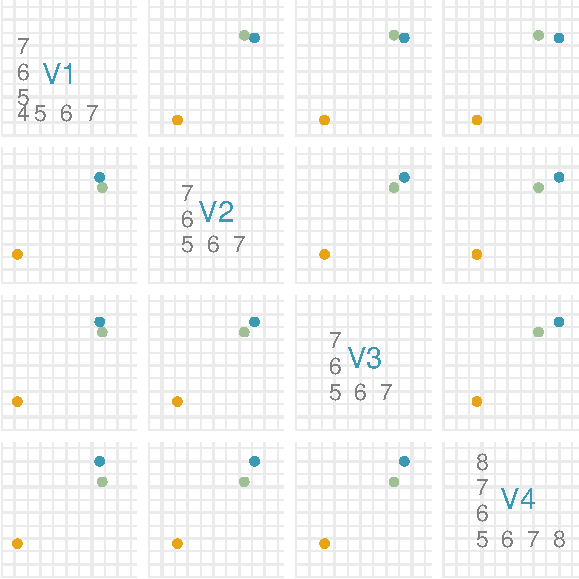
\includegraphics[width=0.8\textwidth,height=\textheight]{6-intro-clust_files/figure-pdf/unnamed-chunk-2-1.pdf}

}

\end{minipage}%
%
\begin{minipage}[t]{0.50\linewidth}

{\centering 

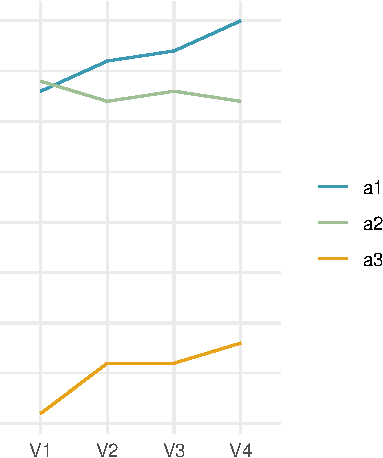
\includegraphics[width=0.8\textwidth,height=\textheight]{6-intro-clust_files/figure-pdf/unnamed-chunk-3-1.pdf}

}

\end{minipage}%

\caption{\label{fig-similarity1}The scatterplot matrix (left) shows that
cases \(a_1\) and \(a_2\) have similar values. The parallel coordinate
plot (right) allows a comparison of other structure, which shows the
similarity in the trend of the profiles on cases \(a_1\) and \(a_3\).}

\end{figure}

\noindent Cases \(a_1\) and \(a_2\) are more similar to each other than
they are to case \(a_3\), because the Euclidean distance between cases
\(a_1\) and \(a_2\) is much smaller than the distance between cases
\(a_1\) and \(a_3\) and between cases \(a_2\) and \(a_3\).

There are many different ways to calculate similarity. Similarity
measures based on correlation distance can be useful. It is typically
used where similarity of structure or shape is more important than
similarity in magnitude.

\index{parallel coordinate plot}

As an example, see the parallel coordinate plot of the sample data at
the right of Figure~\ref{fig-similarity1}. Cases \(a_1\) and \(a_3\) are
widely separated, but their shapes are similar (low, medium, medium,
high). Case \(a_2\), although overlapping with case \(a_1\), has a very
different shape (high, medium, medium, low). The Pearson correlation
between two cases, \(\rho(a_i,a_j)\), is defined as

\begin{align*}
\rho(a_i,a_j) = \frac{(a_i-c_i)^\top(a_j-c_j)}
{\sqrt(a_i-c_i)^\top(a_i-c_i) \sqrt(a_j-c_j)^\top(a_j-c_j)}
\label{corc}
\end{align*}

\noindent Typically, \(c_i, c_j\) are the sample means of each case,
\(\bar{a}_i,\bar{a}_j\). For these three observations,
\(c_1=\bar{a}_1=7.650, c_2=\bar{a}_2=7.275, c_3=\bar{a}_3=4.525\). An
interesting geometric fact, is that if \(c_i, c_j\) are set to be 0, as
is commonly done, \(\rho\) is a generalized correlation that describes
the angle between the two data vectors. The correlation is then
converted to a distance metric, with one possibility being as follows:

\begin{align*}
d_{\rm Cor}(a_i,a_j) = \sqrt{2(1-\rho(a_i,a_j))}
\end{align*}

This distance metric will treat cases that are strongly negatively
correlated as the most distant. If you want to consider strong negative
correlation as close, then you could take the absolute value of
\(\rho(a_i,a_j)\) in the above equation, and remove the multiplication
by 2.

The interpoint distance matrix for the sample data using \(d_{\rm Cor}\)
and the Pearson correlation coefficient is

\begin{align*}
d_{\rm Cor} = \begin{bmatrix}
& {\color{grey} a_1} & {\color{grey} a_2} & {\color{grey} a_3} \\\hline
{\color{grey} a_1} | & 0.0 & 3.6 & 0.1 \\
{\color{grey} a_2} | & 3.6 & 0.0 & 3.8 \\
{\color{grey} a_3} | & 0.1 & 3.8 & 0.0
\end{bmatrix}
\end{align*}

\noindent By this metric, cases \(a_1\) and \(a_3\) are the most
similar, because the correlation distance is smaller between these two
cases than the other pairs of cases.
\index{cluster analysis!interpoint distance}

Note that these interpoint distances differ dramatically from those for
Euclidean distance. As a consequence, the way the cases would be
clustered is also very different. Choosing the appropriate distance
measure is an important part of a cluster analysis.

After a distance metric has been chosen and a cluster analysis has been
performed, the analyst must evaluate the results, and this is actually a
difficult task. A cluster analysis does not generate \(p\)-values or
other numerical criteria, and the process tends to produce hypotheses
rather than testing them. Even the most determined attempts to produce
the ``best'' results using modeling and validation techniques may result
in clusters that, although seemingly significant, are useless for
practical purposes. As a result, cluster analysis is best thought of as
an exploratory technique, and it can be quite useful despite the lack of
formal validation because of its power in data simplification.

Defining an appropriate distance metric from the context of the problem
is a most important decision. For example, if your variables are all
numeric, and on the same scale then Euclidean distance might be best. If
your variables are categorical, you might need to use something like
Hamming distance.

The context in which the data arises is the key to assessing the
results. If the clusters can be characterized in a sensible manner, and
they increase our knowledge of the data, then we are on the right track.
To use an even more pragmatic criterion, if a company can gain an
economic advantage by using a particular clustering method to carve up
their customer database, then that is the method they should use.

\hypertarget{exercises-5}{%
\section*{Exercises}\label{exercises-5}}
\addcontentsline{toc}{section}{Exercises}

\markright{Exercises}

Use the following data to answer these questions:

\begin{verbatim}
     x1   x2   x3
a1 0.13 0.21 0.09
a2 0.91 0.95 0.85
a3 0.62 0.73 0.65
a4 0.21 0.92 0.43
\end{verbatim}

\begin{enumerate}
\def\labelenumi{\arabic{enumi}.}
\item
  Compute the Euclidean distance between cases \texttt{a1}, \texttt{a2},
  \texttt{a3}, \texttt{a4}.
\item
  Compute the correlation distance (as defined above) between cases
  \texttt{a1}, \texttt{a2}, \texttt{a3}, \texttt{a4}.
\item
  Which two points have the (a) biggest (b) smallest Mahalanobis
  (statistical) distance, assuming that the covariance matrix is:
\end{enumerate}

\begin{verbatim}
    x1  x2  x3
x1 1.0 0.8 0.8
x2 0.8 1.0 0.8
x3 0.8 0.8 1.0
\end{verbatim}

(The function \texttt{mahalanobis} will calculate this in R. Technically
this gives distance between each case and the mean vector.)

\begin{enumerate}
\def\labelenumi{\arabic{enumi}.}
\setcounter{enumi}{3}
\item
  Is the ordering of distance between cases the same if Manhattan
  distance is used instead of Euclidean?
\item
  Compute the Chebychev distance between cases \texttt{a1}, \texttt{a2},
  \texttt{a3}, \texttt{a4}.
\item
  Compute Bray-Curtis distance between cases \texttt{a1}, \texttt{a2},
  \texttt{a3}, \texttt{a4}.
\item
  Make a plot of the data, and write a paragraph describing how the
  different distance metrics agree and disagree on how close or far the
  cases are from each other.
\end{enumerate}

\hypertarget{sec-clust-graphics}{%
\chapter{Spin-and-brush approach}\label{sec-clust-graphics}}

\index{brushing!persistent} \index{tour}
\index{cluster analysis!spin-and-brush}

Several examples of the spin-and-brush approach are documented in the
literature, such as Cook et al. (1995a) and Wilhelm et al. (1999). The
steps are:

\begin{enumerate}
\def\labelenumi{\arabic{enumi}.}
\tightlist
\item
  Run the (grand) tour.
\item
  Stop when you see a separated cluster of points.
\item
  Paint the cluster a chosen colour.
\item
  Repeat 1-2 until the data is grouped, and when no other separated
  cluster is visible in any projection. You may need to re-paint some
  points if they appear to be grouped incorrectly in a different
  projection, or paint more points that after spinning most likely
  belong to an existing group.
\end{enumerate}

Spin-and-brush is useful for exploring clustering when the data is
numeric, and contains well-separated clusters. Patterns that adversely
affect numerical techniques, such as nuisance variables or cases,
differences in variances or shapes between clusters, don't pose any
problems for spin-and-brush. It is also effective if the data has
connected low-dimensional (1D or 2D) clusters in high dimensions.

It will not work very well when there are no distinct clusters and the
purpose of clustering is to partition the data into subsets. Here, you
could begin with a solution provided by some numerical clustering
algorithm, and to use visual tools to evaluate it, with goal of refining
the results.

With a complex problem where there are many clusters, one can work
sequentially, and remove each cluster after it is brushed, to de-clutter
the display, in order to find more clusters.

Spin-and-brush is best achieved using a fully interactive graphics
system like in the \texttt{detourr} package, where the results can be
saved for further analysis. The code is very easy, and then all the
controls are interactive.

\begin{Shaded}
\begin{Highlighting}[]
\FunctionTok{library}\NormalTok{(detourr)}
\NormalTok{grDevices}\SpecialCharTok{::}\FunctionTok{hcl.colors}\NormalTok{(}\DecValTok{3}\NormalTok{, }\AttributeTok{palette=}\StringTok{"Zissou 1"}\NormalTok{)}
\FunctionTok{detour}\NormalTok{(penguins\_sub[,}\DecValTok{1}\SpecialCharTok{:}\DecValTok{4}\NormalTok{], }
       \FunctionTok{tour\_aes}\NormalTok{(}\AttributeTok{projection =}\NormalTok{ bl}\SpecialCharTok{:}\NormalTok{bm)) }\SpecialCharTok{|\textgreater{}}
       \FunctionTok{tour\_path}\NormalTok{(}\FunctionTok{grand\_tour}\NormalTok{(}\DecValTok{2}\NormalTok{), }\AttributeTok{fps =} \DecValTok{60}\NormalTok{, }
                 \AttributeTok{max\_bases=}\DecValTok{20}\NormalTok{) }\SpecialCharTok{|\textgreater{}}
       \FunctionTok{show\_scatter}\NormalTok{(}\AttributeTok{alpha =} \FloatTok{0.7}\NormalTok{, }
                    \AttributeTok{axes =} \ConstantTok{FALSE}\NormalTok{)}
\end{Highlighting}
\end{Shaded}

\begin{itemize}
\tightlist
\item
  \texttt{tour\_aes(projection\ =\ bl:bm))} is \texttt{ggplot}-style
  syntax for specifying the variables \texttt{bl:bm} to include in the
  tour.
\item
  \texttt{tour\_path(grand\_tour(2),\ fps\ =\ 60,\ \ \ \ \ \ \ \ \ \ \ \ \ \ \ \ \ \ \ max\_bases=20)}
  specifies 2D grand tour path, with a longer than default path set by
  \texttt{max\_bases=20} and the \texttt{fps} argument sets the
  smoothness.
\item
  Brush interaction is set by choosing the square icon (4th from top),
  so when the cursor is moved over the window points are selected.
\item
  You can choose specific colours to brush, from the colour palette by
  using hexcolours to match your favourite palette. Here we've used
  colours from the Zissou palette.
\item
  The paintbrush icon sets the selected points to the current colour.
\item
  Save the final colour labels using the download icon.
\end{itemize}

\begin{figure}

\begin{minipage}[t]{0.50\linewidth}

{\centering 

\raisebox{-\height}{

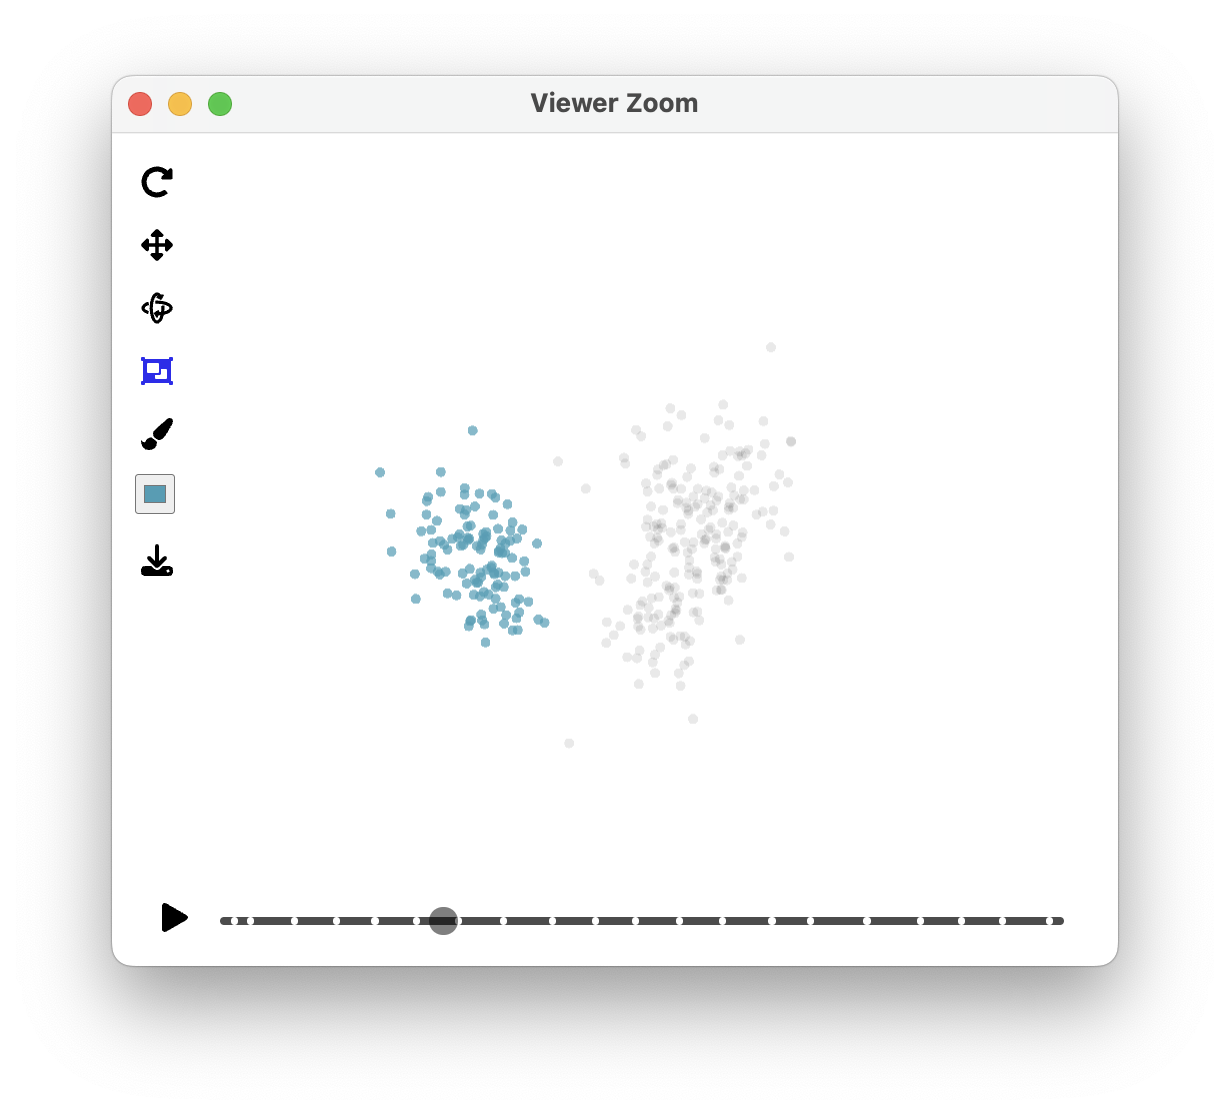
\includegraphics[width=3.125in,height=\textheight]{images/penguins-bs6.png}

}

}

\subcaption{\label{fig-penguins-bs3}One cluster painted}
\end{minipage}%
%
\begin{minipage}[t]{0.50\linewidth}

{\centering 

\raisebox{-\height}{

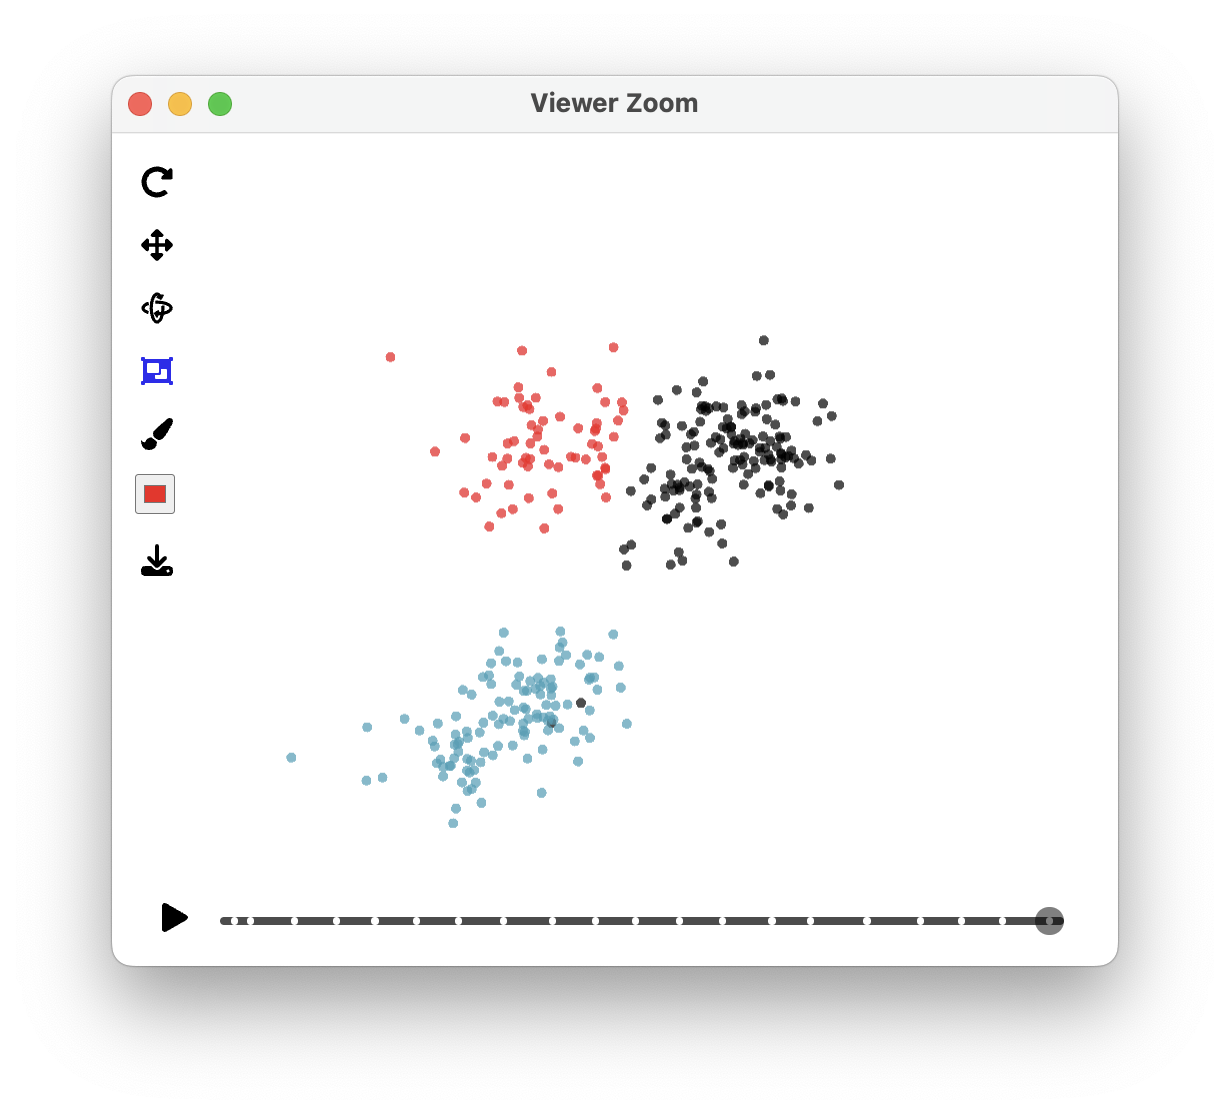
\includegraphics[width=3.125in,height=\textheight]{images/penguins-bs7.png}

}

}

\subcaption{\label{fig-penguins-bs4}Another cluster painted}
\end{minipage}%

\caption{\label{fig-penguins-bs-detourr}Screenshots of the
spin-and-brush approach using \texttt{detourr} on the penguins data.}

\end{figure}

Figure~\ref{fig-penguins-bs-detourr} shows the stages of spin-and-brush
on the penguins data using detourr. The final results can be examined
and used for later analysis. Because this data came with a class
variable, the penguin species, it is interesting to see how close the
spin-and-brush clustering approach came to recovering these:

\begin{Shaded}
\begin{Highlighting}[]
\FunctionTok{library}\NormalTok{(readr)}
\FunctionTok{load}\NormalTok{(}\StringTok{"data/penguins\_sub.rda"}\NormalTok{)}
\NormalTok{detourr\_penguins }\OtherTok{\textless{}{-}} \FunctionTok{read\_csv}\NormalTok{(}\StringTok{"data/detourr\_penguins.csv"}\NormalTok{)}
\FunctionTok{table}\NormalTok{(penguins\_sub}\SpecialCharTok{$}\NormalTok{species, detourr\_penguins}\SpecialCharTok{$}\NormalTok{colour)}
\end{Highlighting}
\end{Shaded}

\begin{verbatim}
           
            000000 3e9eb6 f5191c
  Adelie       143      0      3
  Chinstrap      6      0     62
  Gentoo         2    117      0
\end{verbatim}

It's quite close! All but two of the 119 Gentoo penguins were identified
as a cluster (labelled as ``3e9eb6'' from the chosen light blue hex
colour), and all but three of the 146 Adelie penguins were identified as
a cluster, (labelled as ``000000'' which is the unbrushed black group).
Most of the Chinstrap species were recovered also (labelled as
``f5191c'' for the red hex colour).

\hypertarget{exercises-6}{%
\section*{Exercises}\label{exercises-6}}
\addcontentsline{toc}{section}{Exercises}

\markright{Exercises}

\begin{enumerate}
\def\labelenumi{\arabic{enumi}.}
\tightlist
\item
  Use the spin-and-brush approach to identify the three clusters in the
  \texttt{mulgar::clusters} data set.
\item
  Use the spin-and-brush approach to identify the six clusters in the
  \texttt{mulgar::multicluster} data set. (The code below using detourr
  could be useful.)
\item
  Use spin-and-brush on the challenge data sets, \texttt{c1}-\texttt{c7}
  from the \texttt{mulgar} package. How many clusters do you detect in
  each?
\end{enumerate}

\begin{Shaded}
\begin{Highlighting}[]
\FunctionTok{library}\NormalTok{(detourr)}

\CommentTok{\# Use a random starting basis because the first two variables make it too easy}
\NormalTok{strt }\OtherTok{\textless{}{-}}\NormalTok{ tourr}\SpecialCharTok{::}\FunctionTok{basis\_random}\NormalTok{(}\DecValTok{10}\NormalTok{, }\DecValTok{2}\NormalTok{)}
\FunctionTok{detour}\NormalTok{(multicluster, }
       \FunctionTok{tour\_aes}\NormalTok{(}\AttributeTok{projection =} \SpecialCharTok{{-}}\NormalTok{group)) }\SpecialCharTok{|\textgreater{}}
       \FunctionTok{tour\_path}\NormalTok{(}\FunctionTok{grand\_tour}\NormalTok{(}\DecValTok{2}\NormalTok{), }\AttributeTok{start=}\NormalTok{strt, }\AttributeTok{fps =} \DecValTok{60}\NormalTok{) }\SpecialCharTok{|\textgreater{}}
       \FunctionTok{show\_scatter}\NormalTok{(}\AttributeTok{alpha =} \FloatTok{0.7}\NormalTok{, }\AttributeTok{axes =} \ConstantTok{FALSE}\NormalTok{)}
\end{Highlighting}
\end{Shaded}

\begin{enumerate}
\def\labelenumi{\arabic{enumi}.}
\setcounter{enumi}{2}
\tightlist
\item
  Use the spin-and-brush technique to identify the branches of the
  \texttt{fake\_trees} data available in the \texttt{liminal} package
  (originally from
  \href{https://phate.readthedocs.io/en/stable/}{PHATE}). The result
  should look something like this:
\end{enumerate}

\begin{figure}

{\centering 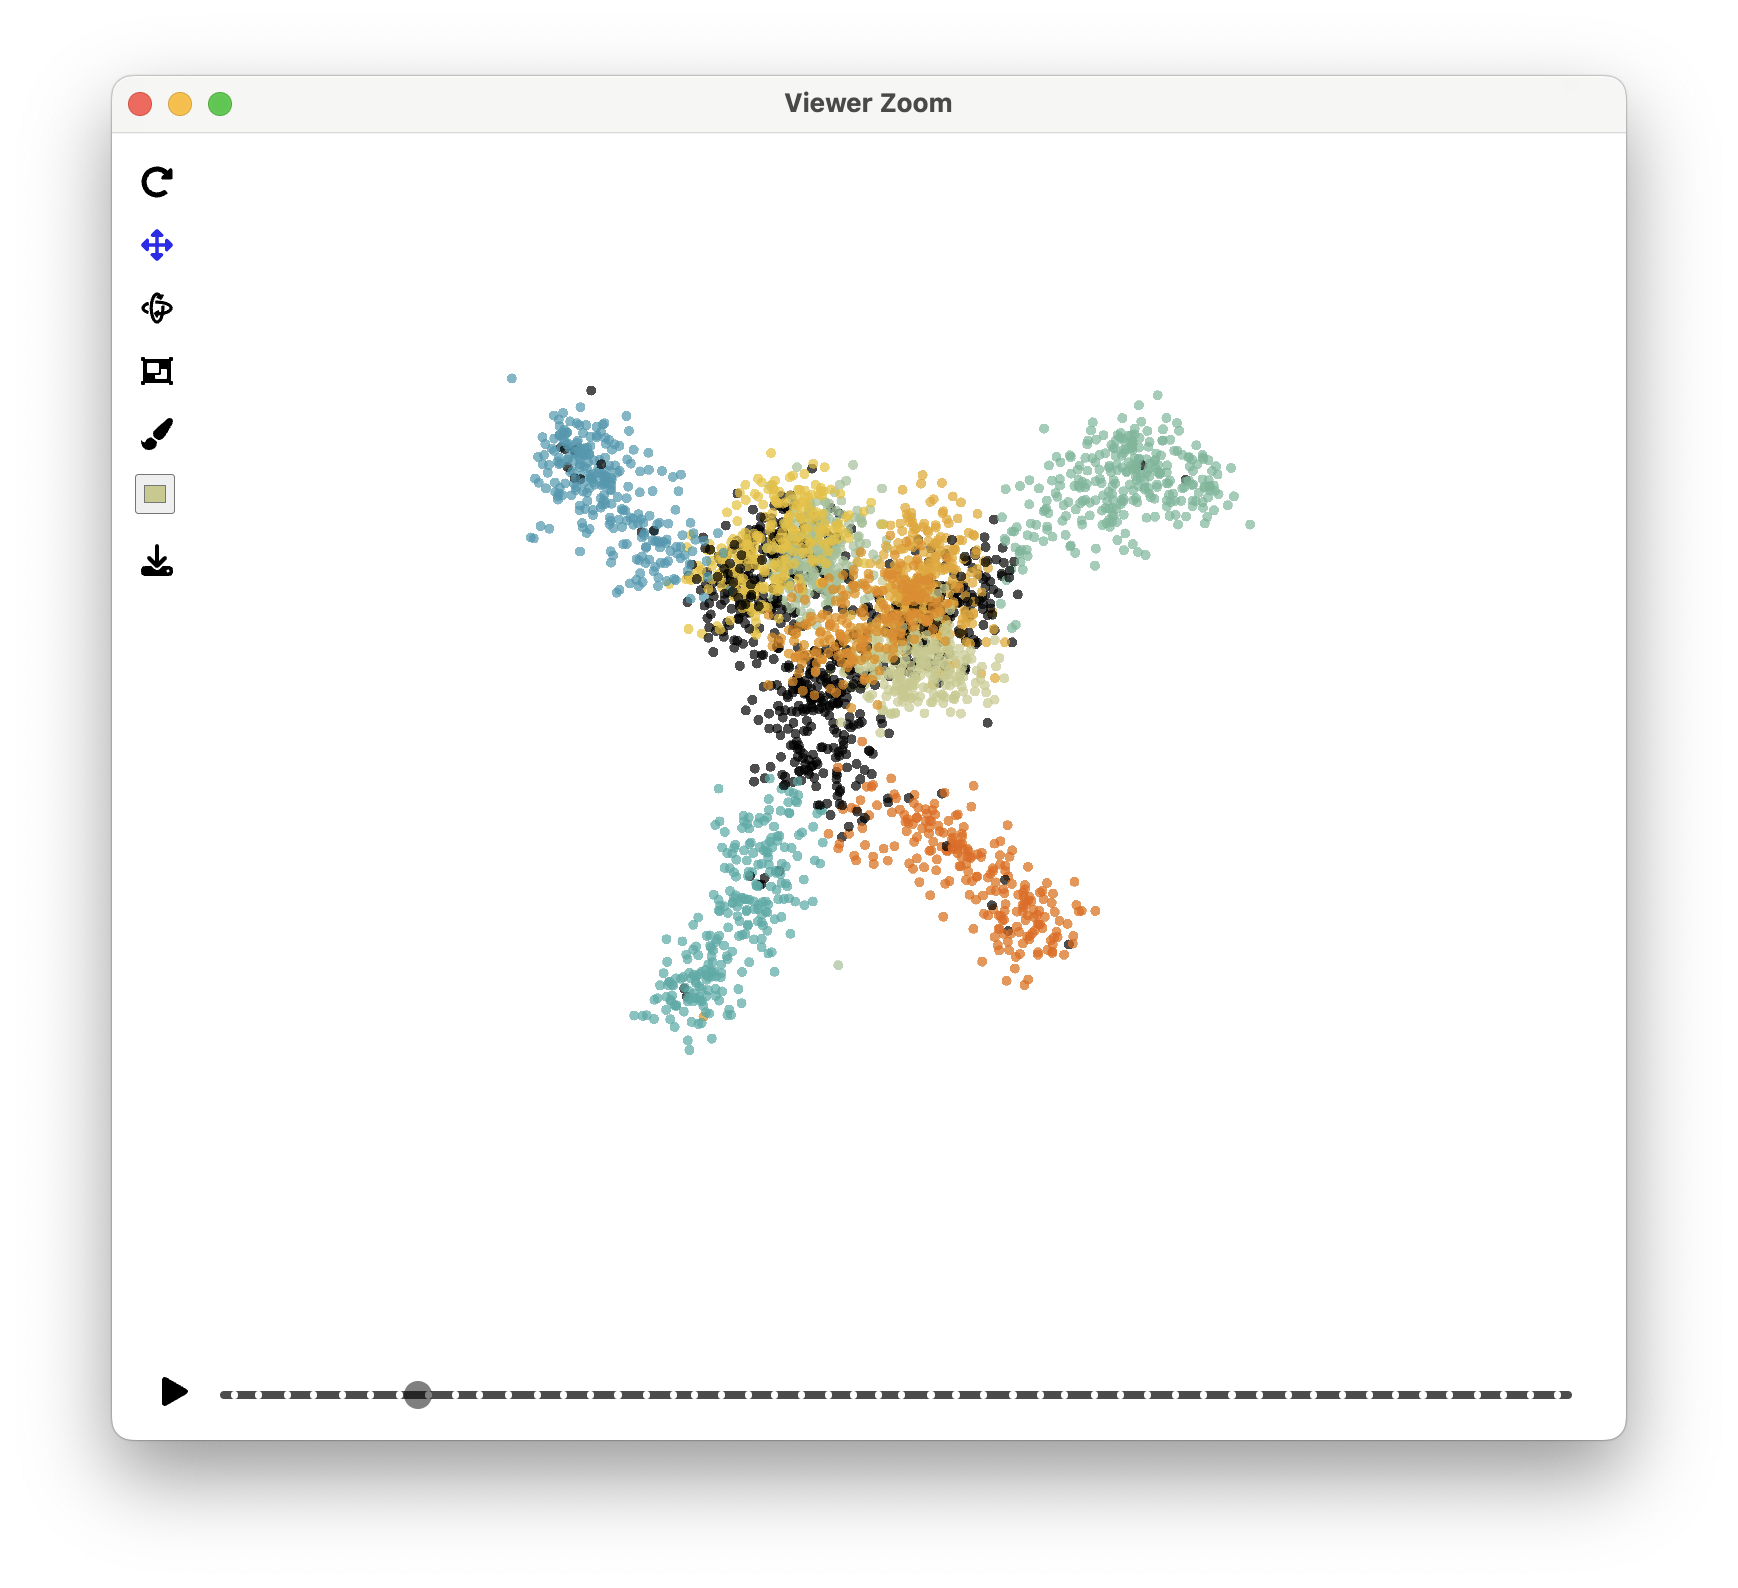
\includegraphics{images/fake_trees_sb.png}

}

\caption{\label{fig-fake-trees-sb}Example solution after spin-and-brush
on fake\_trees data.}

\end{figure}

You can use the download button to save the data with the colours.
Tabulate the \texttt{branches} id variable in the original data with the
\texttt{colour} groups created from brushing, to see how closely you
have recovered the original classes.

\part{Supervised classification}

\hypertarget{overview-1}{%
\chapter{Overview}\label{overview-1}}

Methods for supervised classification originated in the field of
Statistics in the early nineteenth century, under the moniker
\emph{discriminant analysis} (see, for example, Fisher (1936b)). An
increase in the collection of data, and storage in databases, in the
late twentieth century has inspired a growing desire to extract
knowledge from data, particularly to be able accurately predict the
class labels. This has contributed to an explosion of research on new
methods, especially on algorithms that focus on accurate prediction of
new data based on training samples.

\index{classification!supervised}

In contrast to unsupervised classification, the class label (categorical
response variable) is known, in the training sample. The training sample
is used to build the prediction model, and also to estimate the
accuracy, or inversely error, of the model for future data. It is also
important to understand the model and to interpret it, so that we can
know how predictions are made. High-dimensional visualisation can help
with this, and helps to tackle questions like:

\begin{itemize}
\tightlist
\item
  Are the classes well separated in the data space, so that they
  correspond to distinct clusters? If so, what are the shapes of the
  clusters? Is each cluster sufficiently ellipsoidal so that we can
  assume that the data arises from a mixture of multivariate normal
  distributions? Do the clusters exhibit characteristics that suggest
  one algorithm in preference to others?
\item
  Where does the boundary between classes fall? Are the classes linearly
  separable, or does the difference between classes suggest a non-linear
  boundary? How do changes in the input parameters affect these
  boundaries? How do the boundaries generated by different methods vary?
\item
  What cases are misclassified, or have more uncertain predictions? Are
  there places in the data space where predictions are especially good
  or bad?
\item
  Which predictors most contribute to the model predictions? Is it
  possible to reduce the set of explanatory variables?
\end{itemize}

Addressing these types of queries also motivate the emerging field
called explainable artificial intelligence (XAI), which goes beyond
predictive accuracy to more completely satisfy the \emph{desire to
extract knowledge from data}.

Although we focus on categorical response, some of the techniques here
can be modified or adapted for problems with a numeric, or continuous,
response variable. With a categorical response, and numerical
predictors, we map colour to the response variable and use the tour to
examine the relationship between predictors, and the different classes.

\begin{figure}

{\centering 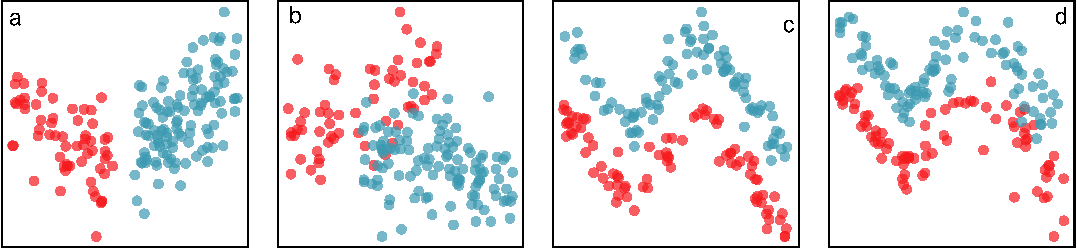
\includegraphics[width=0.8\textwidth,height=\textheight]{13-intro-class_files/figure-pdf/fig-sup-example-1.pdf}

}

\caption{\label{fig-sup-example}Examples of supervised classification
patterns: (a) linearly separable, (b) linear but not completely
separable, (c) non-linearly separable, (d) non-linear, but not
completely separable.}

\end{figure}

Figure~\ref{fig-sup-example} shows some 2D examples where the two
classes are (a) linearly separable, (b) not completely separable but
linearly different, (c) non-linearly separable and (d) not completely
separable but with a non-linear difference. We can also see that in (a)
only the horizontal variable would be important for the model because
the two classes are completely separable in this direction. Although the
pattern in (c) is separable classes, most models would have difficulty
capturing the separation. It is for this reason that it is important to
understand the boundary between classes produced by a fitted model. In
each of b, c, d it is likely that some observations would be
misclassified. Identifying these cases, and inspecting where they are in
the data space is important for understanding the model's future
performance.

\hypertarget{sec-lda}{%
\chapter{Linear discriminant analysis}\label{sec-lda}}

\index{classification!linear discriminant analysis (LDA)}

Linear discriminant analysis (LDA) dates to the early 1900s. It's one of
the most elegant and simple techniques for both modeling separation
between groups, and as an added bonus, producing a low-dimensional
representation of the differences between groups. LDA has two strong
assumptions: the groups are samples from multivariate normal
distributions, and each have the same variance-covariance. If the latter
assumption is relaxed, a slightly less elegant solution results from
quadratic discriminant analysis.

Useful explanations can be found in Venables \& Ripley (2002a) and
Ripley (1996). A good general treatment of parametric methods for
supervised classification can be found in R. A. Johnson \& Wichern
(2002) or another similar multivariate analysis textbook. It's also
useful to know that hypothesis testing for the difference in
multivariate means using multivariate analysis of variance (MANOVA) has
similar assumptions to LDA. Also model-based clustering assumes that
each cluster arises from a multivariate normal distribution, and is
related to LDA. The methods described here can be used to check these
assumptions when applying these methods,
too.\index{classification!multivariate analysis of variance (MANOVA)}
\index{cluster analysis!model-based}

\infobox{Because LDA is a parametric model it is important to check that these assumptions are reasonably satisfied:
\begin{itemize} \itemsep 0in
\item shape of clusters are elliptical.
\item spread of the observations are the same.
\end{itemize}
}

\hypertarget{extracting-the-key-elements-of-the-model}{%
\section{Extracting the key elements of the
model}\label{extracting-the-key-elements-of-the-model}}

LDA builds the model on the between-group sum-of-square matrix

\[B=\sum_{k=1}^g n_k(\bar{X}_k-\bar{X})(\bar{X}_k-\bar{X})^\top\] which
measures the differences between the class means, compared with the
overall data mean \(\bar{X}\) and the within-group sum-of-squares
matrix,

\[
W =
\sum_{k=1}^g\sum_{i=1}^{n_k}
(X_{ki}-\bar{X}_k)(X_{ki}-\bar{X}_k)^\top
\]

which measures the variation of values around each class mean. The
linear discriminant space is generated by computing the eigenvectors
(canonical coordinates) of \(W^{-1}B\), and this is the \((g-1)\)-D
space where the group means are most separated with respect to the
pooled variance-covariance. For each class we compute
\index{classification!discriminant space}

\[
\delta_k(x) = (x-\mu_k)^\top W^{-1}\mu_k + \log \pi_k
\]

where \(\pi_k\) is a prior probability for class \(k\) that might be
based on unequal sample sizes, or cost of misclassification. The LDA
classifier rule is to \emph{assign a new observation to the class with
the largest value} of \(\delta_k(x)\).

We can fit an LDA model using the \texttt{lda()} function from the
\texttt{MASS} package. Here we have used the \texttt{penguins} data,
assuming equal prior probability, to illustrate.

\begin{Shaded}
\begin{Highlighting}[]
\CommentTok{\# Code to fit the model}
\FunctionTok{library}\NormalTok{(dplyr)}
\FunctionTok{library}\NormalTok{(mulgar)}
\FunctionTok{library}\NormalTok{(MASS)}
\FunctionTok{load}\NormalTok{(}\StringTok{"data/penguins\_sub.rda"}\NormalTok{)}

\NormalTok{p\_lda }\OtherTok{\textless{}{-}} \FunctionTok{lda}\NormalTok{(species}\SpecialCharTok{\textasciitilde{}}\NormalTok{bl}\SpecialCharTok{+}\NormalTok{bd}\SpecialCharTok{+}\NormalTok{fl}\SpecialCharTok{+}\NormalTok{bm, }
             \AttributeTok{data=}\NormalTok{penguins\_sub,}
             \AttributeTok{prior=}\FunctionTok{c}\NormalTok{(}\DecValTok{1}\SpecialCharTok{/}\DecValTok{3}\NormalTok{, }\DecValTok{1}\SpecialCharTok{/}\DecValTok{3}\NormalTok{, }\DecValTok{1}\SpecialCharTok{/}\DecValTok{3}\NormalTok{))}
\FunctionTok{options}\NormalTok{(}\AttributeTok{digits=}\DecValTok{2}\NormalTok{)}
\CommentTok{\# p\_lda}
\end{Highlighting}
\end{Shaded}

Because there are three classes the dimension of the discriminant space
is 2D. We can easily extract the group means from the model.

\begin{Shaded}
\begin{Highlighting}[]
\CommentTok{\# Extract the sample means}
\NormalTok{p\_lda}\SpecialCharTok{$}\NormalTok{means}
\end{Highlighting}
\end{Shaded}

\begin{verbatim}
             bl    bd    fl    bm
Adelie    -0.95  0.60 -0.78 -0.62
Chinstrap  0.89  0.64 -0.37 -0.59
Gentoo     0.65 -1.10  1.16  1.10
\end{verbatim}

The coefficients to project the data into the discriminant space, that
is the eigenvectors of \(W^{-1}B\) are:

\begin{Shaded}
\begin{Highlighting}[]
\CommentTok{\# Extract the discriminant space}
\NormalTok{p\_lda}\SpecialCharTok{$}\NormalTok{scaling}
\end{Highlighting}
\end{Shaded}

\begin{verbatim}
     LD1   LD2
bl -0.24 -2.31
bd  2.04  0.19
fl -1.20  0.08
bm -1.22  1.24
\end{verbatim}

and the predicted values, which include class predictions, and
coordinates in the discriminant space are generated as:

\begin{Shaded}
\begin{Highlighting}[]
\CommentTok{\# Extract the fitted values}
\NormalTok{p\_lda\_pred }\OtherTok{\textless{}{-}} \FunctionTok{predict}\NormalTok{(p\_lda, penguins\_sub)}
\end{Highlighting}
\end{Shaded}

The best separation between classes can be viewed from this object,
which can be shown to match the original data projected using the
\texttt{scaling} component of the model object (see
Figure~\ref{fig-p-lda}).

\begin{Shaded}
\begin{Highlighting}[]
\CommentTok{\# Check calculations from the fitted model, and equations}
\FunctionTok{library}\NormalTok{(colorspace)}
\FunctionTok{library}\NormalTok{(ggplot2)}
\FunctionTok{library}\NormalTok{(ggpubr)}
\CommentTok{\# Using the predicted values from the model object}
\NormalTok{p\_lda\_pred\_x1 }\OtherTok{\textless{}{-}} \FunctionTok{data.frame}\NormalTok{(p\_lda\_pred}\SpecialCharTok{$}\NormalTok{x)}
\NormalTok{p\_lda\_pred\_x1}\SpecialCharTok{$}\NormalTok{species }\OtherTok{\textless{}{-}}\NormalTok{ penguins\_sub}\SpecialCharTok{$}\NormalTok{species}
\NormalTok{p\_lda1 }\OtherTok{\textless{}{-}} \FunctionTok{ggplot}\NormalTok{(p\_lda\_pred\_x1, }
                 \FunctionTok{aes}\NormalTok{(}\AttributeTok{x=}\NormalTok{LD1, }\AttributeTok{y=}\NormalTok{LD2, }
                     \AttributeTok{colour=}\NormalTok{species)) }\SpecialCharTok{+} 
  \FunctionTok{geom\_point}\NormalTok{() }\SpecialCharTok{+}
  \FunctionTok{xlim}\NormalTok{(}\SpecialCharTok{{-}}\DecValTok{6}\NormalTok{, }\DecValTok{8}\NormalTok{) }\SpecialCharTok{+} \FunctionTok{ylim}\NormalTok{(}\SpecialCharTok{{-}}\FloatTok{6.5}\NormalTok{, }\FloatTok{5.5}\NormalTok{) }\SpecialCharTok{+}
  \FunctionTok{scale\_color\_discrete\_divergingx}\NormalTok{(}\StringTok{"Zissou 1"}\NormalTok{) }\SpecialCharTok{+}
  \FunctionTok{ggtitle}\NormalTok{(}\StringTok{"(a)"}\NormalTok{) }\SpecialCharTok{+}
  \FunctionTok{theme\_minimal}\NormalTok{() }\SpecialCharTok{+}
  \FunctionTok{theme}\NormalTok{(}\AttributeTok{aspect.ratio =} \DecValTok{1}\NormalTok{, }\AttributeTok{legend.title =} \FunctionTok{element\_blank}\NormalTok{()) }

\CommentTok{\# matches the calculations done manually}
\NormalTok{p\_lda\_pred\_x2 }\OtherTok{\textless{}{-}} \FunctionTok{data.frame}\NormalTok{(}\FunctionTok{as.matrix}\NormalTok{(penguins\_sub[,}\DecValTok{1}\SpecialCharTok{:}\DecValTok{4}\NormalTok{]) }\SpecialCharTok{\%*\%}
\NormalTok{                              p\_lda}\SpecialCharTok{$}\NormalTok{scaling)}
\NormalTok{p\_lda\_pred\_x2}\SpecialCharTok{$}\NormalTok{species }\OtherTok{\textless{}{-}}\NormalTok{ penguins\_sub}\SpecialCharTok{$}\NormalTok{species}
\NormalTok{p\_lda2 }\OtherTok{\textless{}{-}} \FunctionTok{ggplot}\NormalTok{(p\_lda\_pred\_x2, }
                 \FunctionTok{aes}\NormalTok{(}\AttributeTok{x=}\NormalTok{LD1, }\AttributeTok{y=}\NormalTok{LD2, }
                     \AttributeTok{colour=}\NormalTok{species)) }\SpecialCharTok{+} 
  \FunctionTok{geom\_point}\NormalTok{() }\SpecialCharTok{+}
  \FunctionTok{xlim}\NormalTok{(}\SpecialCharTok{{-}}\DecValTok{6}\NormalTok{, }\DecValTok{8}\NormalTok{) }\SpecialCharTok{+} \FunctionTok{ylim}\NormalTok{(}\SpecialCharTok{{-}}\DecValTok{7}\NormalTok{, }\FloatTok{5.5}\NormalTok{) }\SpecialCharTok{+}
  \FunctionTok{scale\_color\_discrete\_divergingx}\NormalTok{(}\StringTok{"Zissou 1"}\NormalTok{) }\SpecialCharTok{+}
  \FunctionTok{ggtitle}\NormalTok{(}\StringTok{"(b)"}\NormalTok{) }\SpecialCharTok{+}
  \FunctionTok{theme\_minimal}\NormalTok{() }\SpecialCharTok{+}
  \FunctionTok{theme}\NormalTok{(}\AttributeTok{aspect.ratio =} \DecValTok{1}\NormalTok{, }\AttributeTok{legend.title =} \FunctionTok{element\_blank}\NormalTok{()) }
\FunctionTok{ggarrange}\NormalTok{(p\_lda1, p\_lda2, }\AttributeTok{ncol=}\DecValTok{2}\NormalTok{, }
          \AttributeTok{common.legend =} \ConstantTok{TRUE}\NormalTok{, }\AttributeTok{legend =} \StringTok{"bottom"}\NormalTok{)}
\end{Highlighting}
\end{Shaded}

\begin{figure}[H]

{\centering 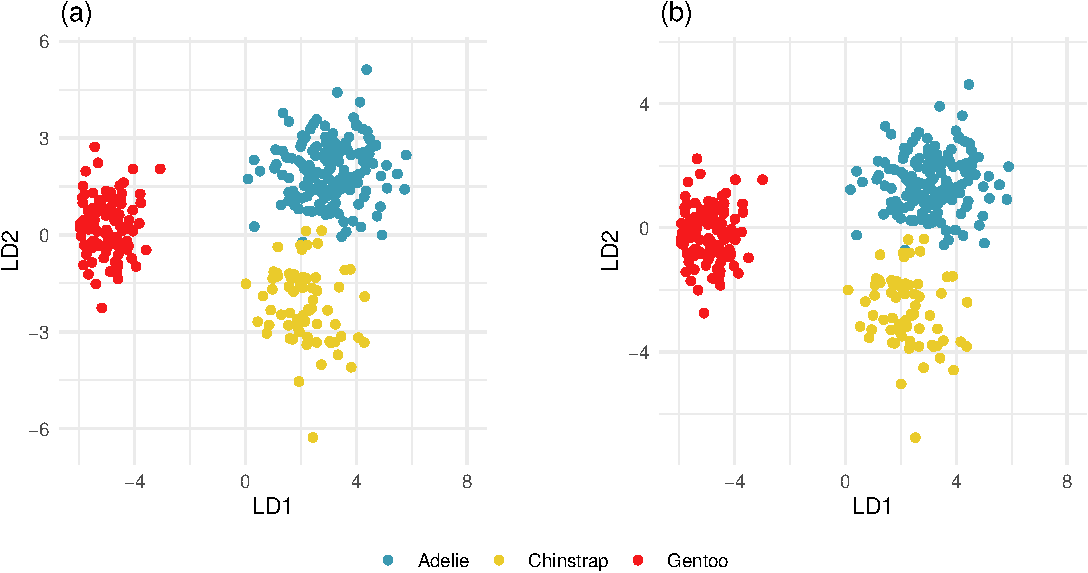
\includegraphics[width=0.8\textwidth,height=\textheight]{14-lda_files/figure-pdf/fig-p-lda-1.pdf}

}

\caption{\label{fig-p-lda}Penguins projected into the 2D discriminant
space, done two ways: (a) using the predicted values, (b) directly
projecting using the model component. The scale is not quite the same
but the projected data is identical in shape.}

\end{figure}

The \(W\) and \(B\) matrices cannot be extracted from the model object,
so we need to compute these separately. We only need \(W\) actually. It
is useful to think of this as the pooled variance-covariance matrix.
Because the assumption for LDA is that the population group
variance-covariances are identical, we estimate this by computing them
for each class and then averaging them to get the pooled
variance-covariance matrix. It's laborious, but easy.

\begin{Shaded}
\begin{Highlighting}[]
\CommentTok{\# Compute pooled variance{-}covariance}
\NormalTok{p\_vc\_pool }\OtherTok{\textless{}{-}}\NormalTok{ mulgar}\SpecialCharTok{::}\FunctionTok{pooled\_vc}\NormalTok{(penguins\_sub[,}\DecValTok{1}\SpecialCharTok{:}\DecValTok{4}\NormalTok{],}
\NormalTok{                               penguins\_sub}\SpecialCharTok{$}\NormalTok{species)}
\NormalTok{p\_vc\_pool}
\end{Highlighting}
\end{Shaded}

\begin{verbatim}
     bl   bd   fl   bm
bl 0.31 0.18 0.13 0.18
bd 0.18 0.32 0.14 0.20
fl 0.13 0.14 0.23 0.16
bm 0.18 0.20 0.16 0.31
\end{verbatim}

This can be used to draw an ellipse corresponding to the pooled
variance-covariance that is used by the LDA model.

\hypertarget{checking-assumptions}{%
\section{Checking assumptions}\label{checking-assumptions}}

This LDA approach is widely applicable, but it is useful to check the
underlying assumptions on which it depends: (1) that the cluster
structure corresponding to each class forms an ellipse, showing that the
class is consistent with a sample from a multivariate normal
distribution, and (2) that the variance of values around each mean is
nearly the same. Figure~\ref{fig-lda-assumptions1} and
Figure~\ref{fig-lda-assumptions2} illustrates two datasets, of which
only one is consistent with these assumptions. Other parametric models,
such as quadratic discriminant analysis or logistic regression, also
depend on assumptions about the data which should be validated.
\index{classification!quadratic discriminant analysis (QDA)}
\index{classification!logistic regression}

\infobox{To check the equal and elliptical variance-covariance assumption, generate points on the surface of an ellipse corresponding to the variance-covariance for each group. When watching these ellipses in a tour, they should similar in all projections.
}

\index{classification!variance-covariance} \index{variance-covariance}

\begin{Shaded}
\begin{Highlighting}[]
\CommentTok{\# Generate ellipses for each group\textquotesingle{}s variance{-}covariance}
\NormalTok{p\_ell }\OtherTok{\textless{}{-}} \ConstantTok{NULL}
\ControlFlowTok{for}\NormalTok{ (i }\ControlFlowTok{in} \FunctionTok{unique}\NormalTok{(penguins\_sub}\SpecialCharTok{$}\NormalTok{species)) \{}
\NormalTok{  x }\OtherTok{\textless{}{-}}\NormalTok{ penguins\_sub }\SpecialCharTok{\%\textgreater{}\%}\NormalTok{ dplyr}\SpecialCharTok{::}\FunctionTok{filter}\NormalTok{(species }\SpecialCharTok{==}\NormalTok{ i)}
\NormalTok{  e }\OtherTok{\textless{}{-}} \FunctionTok{gen\_xvar\_ellipse}\NormalTok{(x[,}\DecValTok{1}\SpecialCharTok{:}\DecValTok{2}\NormalTok{], }\AttributeTok{n=}\DecValTok{150}\NormalTok{, }\AttributeTok{nstd=}\FloatTok{1.5}\NormalTok{)}
\NormalTok{  e}\SpecialCharTok{$}\NormalTok{species }\OtherTok{\textless{}{-}}\NormalTok{ i}
\NormalTok{  p\_ell }\OtherTok{\textless{}{-}} \FunctionTok{bind\_rows}\NormalTok{(p\_ell, e)}
\NormalTok{\}}
\end{Highlighting}
\end{Shaded}

\begin{figure}

{\centering 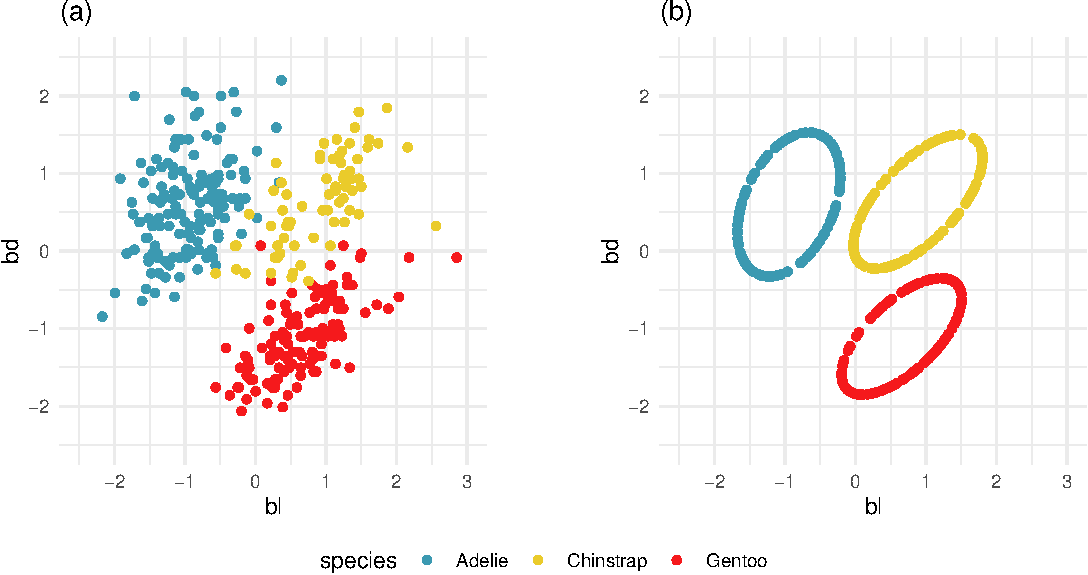
\includegraphics[width=0.8\textwidth,height=\textheight]{14-lda_files/figure-pdf/fig-lda-assumptions1-1.pdf}

}

\caption{\label{fig-lda-assumptions1}Scatterplot of flipper length by
bill length of the penguins data, and corresponding variance-covariance
ellipses. There is a small amount of difference between the ellipses,
but they are similar enough to be confident in assuming the population
variance-covariances are equal.}

\end{figure}

\begin{figure}

{\centering 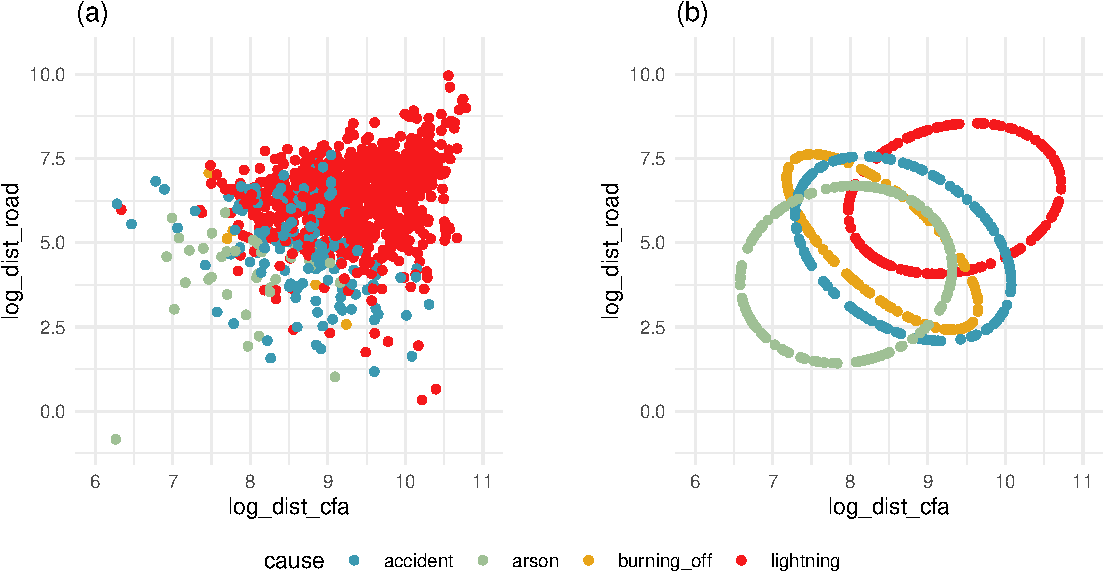
\includegraphics[width=0.8\textwidth,height=\textheight]{14-lda_files/figure-pdf/fig-lda-assumptions2-1.pdf}

}

\caption{\label{fig-lda-assumptions2}Scatterplot of distance to cfa and
road for the bushfires data, and corresponding variance-covariance
ellipses. There is a lot of difference between the ellipses, so it
cannot be assumed that the population variance-covariances are equal.}

\end{figure}

\index{data!bushfires}

\insightbox{The equal and elliptical variance-covariance assumption is reasonable for the penguins data because the ellipse shapes roughly match the spread of the data. It is not a suitable assumption for the bushfires data, because the spread is not elliptically-shaped and varies in size between groups.}

This approach extends to any dimension. We would use the same projection
sequence to view both the data and the variance-covariance ellipses, as
in Figure~\ref{fig-penguins-lda-ellipses-pdf}. It can be seen that there
is some difference in the shape and size of the ellipses between
species, in some projections, and also with the spread of points in the
projected data. However, it is the differences are small, so it would be
safe to assume that the population variance-covariances are equal.

\begin{figure}

\begin{minipage}[t]{0.50\linewidth}

{\centering 

\raisebox{-\height}{

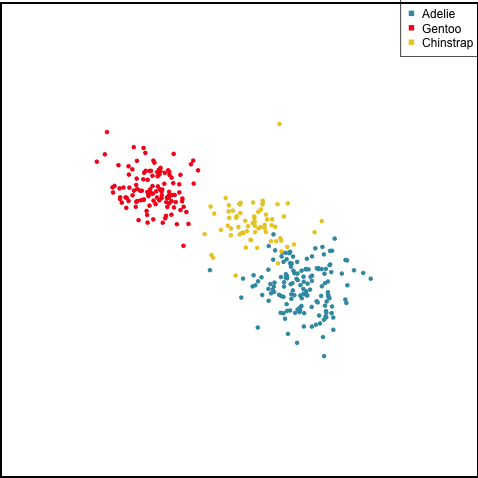
\includegraphics{images/penguins_lda1.png}

}

}

\subcaption{\label{fig-lda-4D-assumptions1}Data}
\end{minipage}%
%
\begin{minipage}[t]{0.50\linewidth}

{\centering 

\raisebox{-\height}{

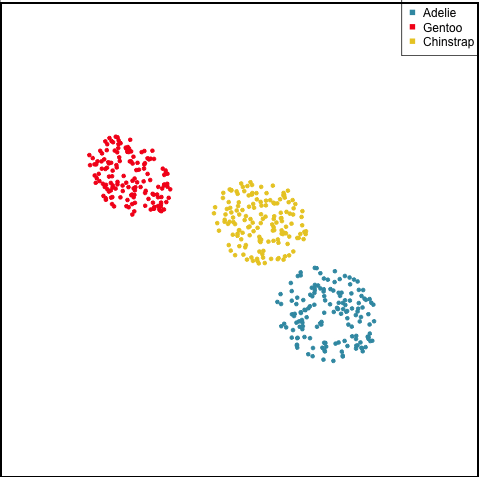
\includegraphics{images/penguins_lda2.png}

}

}

\subcaption{\label{fig-lda-4D-assumptions2}Variance-covariance ellipses}
\end{minipage}%

\caption{\label{fig-penguins-lda-ellipses-pdf}Checking the assumption of
equal variance-covariance matrices for the 4D penguins data. Each
ellipse corresponds to the sample variance-covariance for each species.}

\end{figure}

As a further check, we could generate three ellipses corresponding to
the pooled variance-covariance matrix, as would be used in the model,
centered at each of the means. Overlay this with the data, as done in
Figure~\ref{fig-penguins-lda-pooled-pdf}. Now you will compare the
spread of the observations in the data, with the elliptical shape of the
pooled variance-covariance. If it matches reasonably we can safely use
LDA. This can also be done group by group when multiple groups make it
difficult to view all together.

\infobox{To check the fit of the equal variance-covariance assumption, simulate points on the ellipse corresponding to the \emph{pooled sample variance-covariance matrix}. Generate one for each group centered at the group mean, and compare with the data.}

\index{classification!pooled variance-covariance}
\index{pooled variance-covariance}

\begin{Shaded}
\begin{Highlighting}[]
\CommentTok{\# Create an ellipse corresponding to pooled vc}
\NormalTok{pool\_ell }\OtherTok{\textless{}{-}} \FunctionTok{gen\_vc\_ellipse}\NormalTok{(p\_vc\_pool, }
                           \AttributeTok{xm=}\FunctionTok{rep}\NormalTok{(}\DecValTok{0}\NormalTok{, }\FunctionTok{ncol}\NormalTok{(p\_vc\_pool)))}

\CommentTok{\# Add means to produce ellipses for each species}
\NormalTok{p\_lda\_pool }\OtherTok{\textless{}{-}} \FunctionTok{data.frame}\NormalTok{(}\FunctionTok{rbind}\NormalTok{(}
\NormalTok{  pool\_ell }\SpecialCharTok{+}
    \FunctionTok{matrix}\NormalTok{(}\FunctionTok{rep}\NormalTok{(p\_lda}\SpecialCharTok{$}\NormalTok{means[}\DecValTok{1}\NormalTok{,],}
      \AttributeTok{each=}\FunctionTok{nrow}\NormalTok{(pool\_ell)), }\AttributeTok{ncol=}\DecValTok{4}\NormalTok{),}
\NormalTok{  pool\_ell }\SpecialCharTok{+}
    \FunctionTok{matrix}\NormalTok{(}\FunctionTok{rep}\NormalTok{(p\_lda}\SpecialCharTok{$}\NormalTok{means[}\DecValTok{2}\NormalTok{,],}
      \AttributeTok{each=}\FunctionTok{nrow}\NormalTok{(pool\_ell)), }\AttributeTok{ncol=}\DecValTok{4}\NormalTok{),}
\NormalTok{  pool\_ell }\SpecialCharTok{+}
    \FunctionTok{matrix}\NormalTok{(}\FunctionTok{rep}\NormalTok{(p\_lda}\SpecialCharTok{$}\NormalTok{means[}\DecValTok{3}\NormalTok{,],}
      \AttributeTok{each=}\FunctionTok{nrow}\NormalTok{(pool\_ell)), }\AttributeTok{ncol=}\DecValTok{4}\NormalTok{)))}
\CommentTok{\# Create one data set with means, data, ellipses}
\NormalTok{p\_lda\_pool}\SpecialCharTok{$}\NormalTok{species }\OtherTok{\textless{}{-}} \FunctionTok{factor}\NormalTok{(}\FunctionTok{rep}\NormalTok{(}\FunctionTok{levels}\NormalTok{(penguins\_sub}\SpecialCharTok{$}\NormalTok{species),}
                          \FunctionTok{rep}\NormalTok{(}\FunctionTok{nrow}\NormalTok{(pool\_ell), }\DecValTok{3}\NormalTok{)))}
\NormalTok{p\_lda\_pool}\SpecialCharTok{$}\NormalTok{type }\OtherTok{\textless{}{-}} \StringTok{"ellipse"}
\NormalTok{p\_lda\_means }\OtherTok{\textless{}{-}} \FunctionTok{data.frame}\NormalTok{(}
\NormalTok{  p\_lda}\SpecialCharTok{$}\NormalTok{means,}
  \AttributeTok{species=}\FunctionTok{factor}\NormalTok{(}\FunctionTok{rownames}\NormalTok{(p\_lda}\SpecialCharTok{$}\NormalTok{means)),}
                          \AttributeTok{type=}\StringTok{"mean"}\NormalTok{)}
\NormalTok{p\_data }\OtherTok{\textless{}{-}} \FunctionTok{data.frame}\NormalTok{(penguins\_sub[,}\DecValTok{1}\SpecialCharTok{:}\DecValTok{5}\NormalTok{], }
                     \AttributeTok{type=}\StringTok{"data"}\NormalTok{)}
\NormalTok{p\_lda\_all }\OtherTok{\textless{}{-}} \FunctionTok{bind\_rows}\NormalTok{(p\_lda\_means,}
\NormalTok{                       p\_data,}
\NormalTok{                       p\_lda\_pool)}
\NormalTok{p\_lda\_all}\SpecialCharTok{$}\NormalTok{type }\OtherTok{\textless{}{-}} \FunctionTok{factor}\NormalTok{(p\_lda\_all}\SpecialCharTok{$}\NormalTok{type, }
   \AttributeTok{levels=}\FunctionTok{c}\NormalTok{(}\StringTok{"mean"}\NormalTok{, }\StringTok{"data"}\NormalTok{, }\StringTok{"ellipse"}\NormalTok{))}
\NormalTok{shapes }\OtherTok{\textless{}{-}} \FunctionTok{c}\NormalTok{(}\DecValTok{3}\NormalTok{, }\DecValTok{4}\NormalTok{, }\DecValTok{20}\NormalTok{)}
\NormalTok{p\_pch }\OtherTok{\textless{}{-}}\NormalTok{ shapes[p\_lda\_all}\SpecialCharTok{$}\NormalTok{type]}
\end{Highlighting}
\end{Shaded}

\begin{figure}

\begin{minipage}[t]{0.50\linewidth}

{\centering 

\raisebox{-\height}{

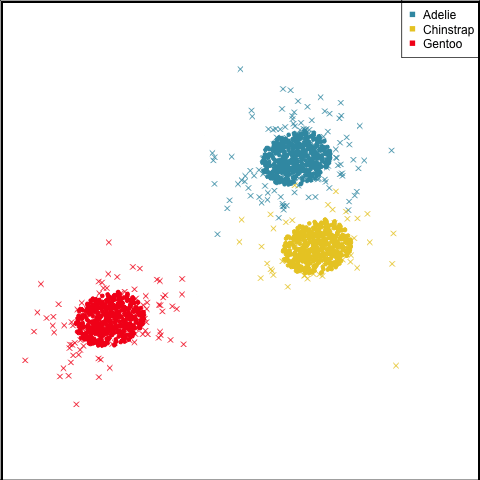
\includegraphics{images/penguins_lda_pooled1.png}

}

}

\subcaption{\label{fig-lda-pooled1}All species}
\end{minipage}%
%
\begin{minipage}[t]{0.50\linewidth}

{\centering 

\raisebox{-\height}{

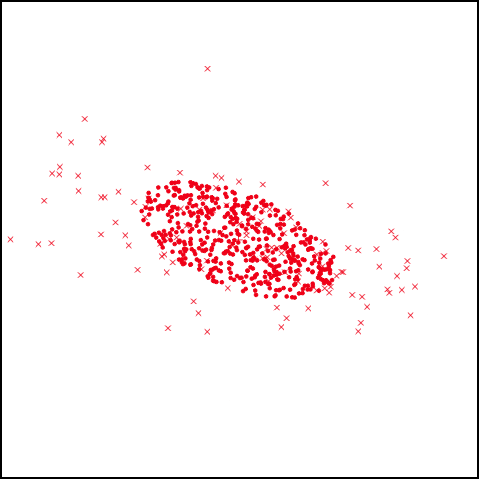
\includegraphics{images/penguins_lda_pooled2.png}

}

}

\subcaption{\label{fig-lda-pooled1}Gentoo}
\end{minipage}%

\caption{\label{fig-penguins-lda-pooled-pdf}Checking how the pooled
variance-covariance matches the spread of points in each group.}

\end{figure}

\insightbox{From the tour, we can see that the assumption of equal elliptical variance-covariance is a reasonable assumption for the penguins data. In all projections the ellipse is reasonably matching the spread of the observations.
}

\hypertarget{examining-results}{%
\section{Examining results}\label{examining-results}}

The boundaries for a classification model can be examined by:

\begin{enumerate}
\def\labelenumi{\arabic{enumi}.}
\tightlist
\item
  generating a large number of test points in the domain of the data
\item
  predicting the class for each test point
\end{enumerate}

We'll look at this for 2D using the LDA model fitted to \texttt{bl}, and
\texttt{bd} of the \texttt{penguins} data.

\begin{Shaded}
\begin{Highlighting}[]
\NormalTok{p\_bl\_bd\_lda }\OtherTok{\textless{}{-}} \FunctionTok{lda}\NormalTok{(species}\SpecialCharTok{\textasciitilde{}}\NormalTok{bl}\SpecialCharTok{+}\NormalTok{bd, }\AttributeTok{data=}\NormalTok{penguins\_sub, }
                                  \AttributeTok{prior =} \FunctionTok{c}\NormalTok{(}\DecValTok{1}\SpecialCharTok{/}\DecValTok{3}\NormalTok{, }\DecValTok{1}\SpecialCharTok{/}\DecValTok{3}\NormalTok{, }\DecValTok{1}\SpecialCharTok{/}\DecValTok{3}\NormalTok{))}
\end{Highlighting}
\end{Shaded}

The fitted model means \(\bar{x}_{Adelie} = (\) -0.95, 0.6\()^\top\),
\(\bar{x}_{Chinstrap} = (\) 0.89, 0.64\()^\top\), and
\(\bar{x}_{Gentoo} = (\) 0.65, -1.1\()^\top\) can be added to the plots.

The boundaries can be examined using the \texttt{explore()} function
from the \texttt{classifly} package, which generates observations in the
range of all values of\texttt{bl} and \texttt{bd} and predicts their
class. Figure~\ref{fig-lda-2D-boundary} shows the resulting prediction
regions, with the observed data and the sample means overlaid.

\begin{Shaded}
\begin{Highlighting}[]
\CommentTok{\# Compute points in domain of data and predict}
\FunctionTok{library}\NormalTok{(classifly)}

\NormalTok{p\_bl\_bd\_lda\_boundaries }\OtherTok{\textless{}{-}} \FunctionTok{explore}\NormalTok{(p\_bl\_bd\_lda, penguins\_sub)}
\NormalTok{p\_bl\_bd\_lda\_m1 }\OtherTok{\textless{}{-}} \FunctionTok{ggplot}\NormalTok{(p\_bl\_bd\_lda\_boundaries) }\SpecialCharTok{+}
  \FunctionTok{geom\_point}\NormalTok{(}\FunctionTok{aes}\NormalTok{(}\AttributeTok{x=}\NormalTok{bl, }\AttributeTok{y=}\NormalTok{bd, }
                 \AttributeTok{colour=}\NormalTok{species, }
                 \AttributeTok{shape=}\NormalTok{.TYPE), }\AttributeTok{alpha=}\FloatTok{0.8}\NormalTok{) }\SpecialCharTok{+} 
  \FunctionTok{scale\_color\_discrete\_divergingx}\NormalTok{(}\StringTok{"Zissou 1"}\NormalTok{) }\SpecialCharTok{+}
  \FunctionTok{scale\_shape\_manual}\NormalTok{(}\AttributeTok{values=}\FunctionTok{c}\NormalTok{(}\DecValTok{46}\NormalTok{, }\DecValTok{16}\NormalTok{)) }\SpecialCharTok{+}
  \FunctionTok{theme\_minimal}\NormalTok{() }\SpecialCharTok{+}
  \FunctionTok{theme}\NormalTok{(}\AttributeTok{aspect.ratio =} \DecValTok{1}\NormalTok{, }\AttributeTok{legend.position =} \StringTok{"none"}\NormalTok{)}

\NormalTok{p\_bl\_bd\_lda\_means }\OtherTok{\textless{}{-}} \FunctionTok{data.frame}\NormalTok{(p\_bl\_bd\_lda}\SpecialCharTok{$}\NormalTok{means,}
                        \AttributeTok{species=}\FunctionTok{rownames}\NormalTok{(p\_bl\_bd\_lda}\SpecialCharTok{$}\NormalTok{means))}
\NormalTok{p\_bl\_bd\_lda\_m1 }\SpecialCharTok{+}   
  \FunctionTok{geom\_point}\NormalTok{(}\AttributeTok{data=}\NormalTok{p\_bl\_bd\_lda\_means, }
             \FunctionTok{aes}\NormalTok{(}\AttributeTok{x=}\NormalTok{bl, }\AttributeTok{y=}\NormalTok{bd), }
             \AttributeTok{colour=}\StringTok{"black"}\NormalTok{, }
             \AttributeTok{shape=}\DecValTok{3}\NormalTok{,}
             \AttributeTok{size=}\DecValTok{3}\NormalTok{) }
\end{Highlighting}
\end{Shaded}

\begin{figure}[H]

{\centering 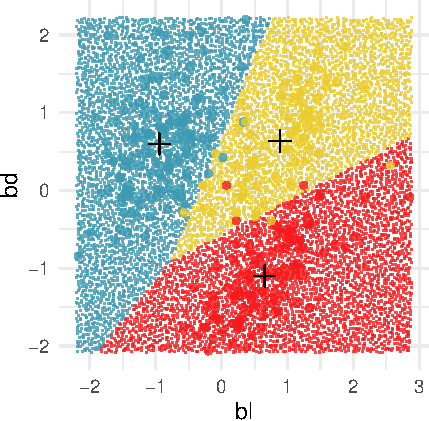
\includegraphics[width=0.7\textwidth,height=\textheight]{14-lda_files/figure-pdf/fig-lda-2D-boundary-1.pdf}

}

\caption{\label{fig-lda-2D-boundary}Prediction regions of the LDA model
for two variables of the three species of penguins indicated by the
small points. Large points are the observations, and the sample mean of
each species is represented by the plus. The boundaries between groups
can be seen to be roughly half-way between the means, taking the
elliptical spread into account, and mostly distinguishes the three
species.}

\end{figure}

\index{classification!boundaries}

This approach can be readily extended to higher dimensions. One first
fits the model with all four variables, and uses the \texttt{explore()}
to generate points in the 4D space with predictions, generating a
representation of the prediction regions.
Figure~\ref{fig-penguins-lda-boundaries-pdf}(a) shows the results.
Points inside the slice are shown in larger size. The slice is made in
the centre of the data, to show the boundaries in this neighbourhood. As
the tour progresses we see a thin slice through the centre of the data,
parallel with the projection plane. In most projections there is some
small overlap of points between groups, which happens because we are
examining a 4D object with 2D. The slice helps ot alleviate this,
allowing a focus on the boundaries in the centre of the cube. In all
projections the boundaries between groups is linear, as would be
expected when using LDA. We can also see that the model roughly divides
the cube into three relatively equally-sized regions.

Figure~\ref{fig-penguins-lda-boundaries-pdf}(b) shows the three
prediction regions, represented by points in 4D, projected into the
discriminant space. Linear boundaries neatly divide the full space,
which is to be expected because the LDA model computes it's
classification rules in this 2D space.\\
\index{classification!discriminant space}

\begin{figure}

\begin{minipage}[t]{0.50\linewidth}

{\centering 

\raisebox{-\height}{

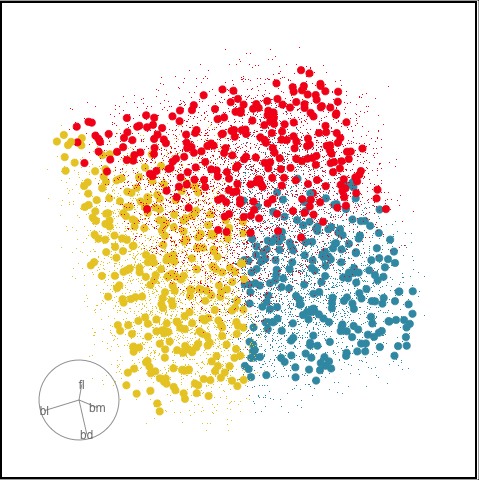
\includegraphics[width=2.08333in,height=\textheight]{images/penguins_lda_boundaries.png}

}

}

\subcaption{\label{fig-lda-4D-boundaries}4D}
\end{minipage}%
%
\begin{minipage}[t]{0.50\linewidth}

{\centering 

\raisebox{-\height}{

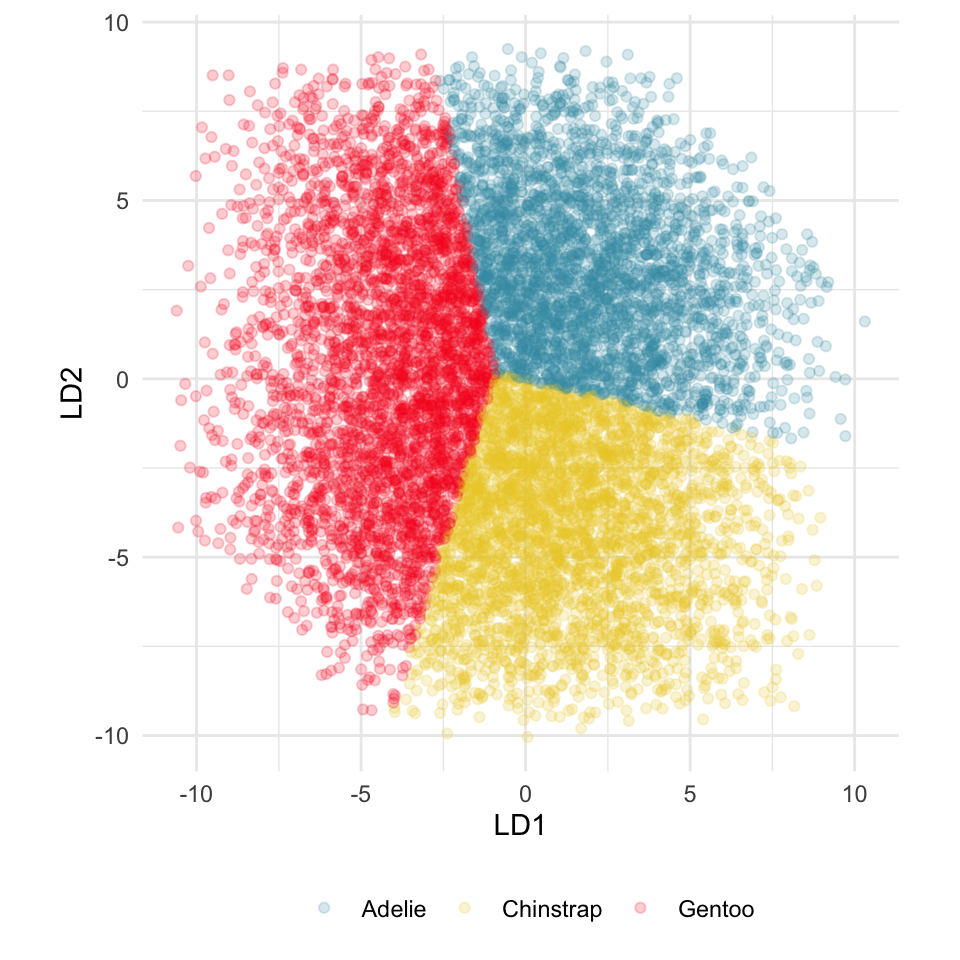
\includegraphics[width=2.08333in,height=\textheight]{images/fig-lda-2D-boundaries-1.png}

}

}

\subcaption{\label{fig-lda-4D-ds}Discriminant space}
\end{minipage}%
\newline
\begin{minipage}[t]{0.50\linewidth}

{\centering 

}

\end{minipage}%

\caption{\label{fig-penguins-lda-boundaries-pdf}Examining the boundaries
produced by the LDA model in the full 4D with a slice tour (left shows a
single frame) and in the discriminant space (right). Large points
indicate observations within the slice, and dots are observations
outside the slice. Focusing on the within-slice points, there is some
overlap of points between regions in most views which represents the
occlusion of 4D shapes when examining projections with thin slices. The
linear boundaries are seen exactly in the discriminant space, that is
they are orthogonal to these two dimensions.}

\end{figure}

\insightbox{From the tour, we can see that the LDA boundaries divide the classes only in the discriminant space. It is not using the space orthogonal to the 2D discriminant space. You can see this because the boundary is sharp in just one 2D projection, while most of the projections show some overlap of regions.}

\hypertarget{exercises-7}{%
\section*{Exercises}\label{exercises-7}}
\addcontentsline{toc}{section}{Exercises}

\markright{Exercises}

\begin{enumerate}
\def\labelenumi{\arabic{enumi}.}
\tightlist
\item
  For the \texttt{simple\_clusters} compute the LDA model, and make a
  plot of the data, with points coloured by the class. Overlay
  variance-covariance ellipses, and a \(+\) indicating the sample mean
  for each class. Is it reasonable to assume that the two classes are
  sampled from populations with the same variance-covariance?
\item
  Examine the clusters corresponding to the classes in the
  \texttt{clusters} data set, using a tour. Based on the shape of the
  data is the assumption of equal variance-covariance reasonable?
\item
  Examine the pooled variance-covariance for the \texttt{clusters} data,
  overlaid on the data in a tour on the 5D. Does it fit the variance of
  each cluster nicely?
\item
  Fit an LDA model to the \texttt{simple\_clusters} data. Examine the
  boundaries produced by the model, in 2D.
\item
  Fit an LDA model to the \texttt{clusters} data. Examine the boundaries
  produced by the model in 5D.
\item
  Assess the LDA assumptions for the \texttt{multicluster} data. Is LDA
  an appropriate model?
\item
  Compute the first 12 PCs of the \texttt{sketches} data. Check the
  assumption of equal, elliptical variance-covariance of the 6 groups.
  Regardless of whether you decide that the assumption is satisfied or
  not, fit an LDA to the 12 PCs. Extract the discriminant space (the
  \texttt{x} component of the \texttt{predict} object), and examine the
  separation (or not) of the 6 groups in this 5D space. Is LDA providing
  a good classification model for this data?
\item
  Even though the \texttt{bushfires} data does not satisfy the
  assumptions for LDA, fit LDA to the first five PCs. Examine the class
  differences in the 3D discriminant space.
\item
  Compute the boundary between classes, for the LDA model where the
  prior probability reflects the sample size, and the LDA model where
  the priors are equal for all groups. How does the boundary between
  lightning caused fires and the other groups change?
\end{enumerate}

\hypertarget{sec-trees-forests}{%
\chapter{Trees and forests}\label{sec-trees-forests}}

\hypertarget{sec-trees}{%
\section{Trees}\label{sec-trees}}

\index{classification!trees}

The tree algorithm (Breiman et al., 1984) is a simple and versatile
algorithmic method for supervised classification. The basic tree
algorithm generates a classification rule by sequentially splitting the
data into two buckets. Splits are made between sorted data values of
individual variables, with the goal of obtaining pure classes on each
side of the split. The inputs for a simple tree classifier commonly
include (1) an impurity measure, an indication of the relative diversity
among the cases in the terminal nodes; (2) a parameter that sets the
minimum number of cases in a node, or the minimum number of observations
in a terminal node of the tree; and (3) a complexity measure that
controls the growth of a tree, balancing the use of a simple
generalizable tree against a more accurate tree tailored to the sample.
When applying tree methods, exploring the effects of the input
parameters on the tree is instructive; for example, it helps us to
assess the stability of the tree model.

Although algorithmic models do not depend on distributional assumptions,
that does not mean that every algorithm is suitable for all data. For
example, the tree model works best when all variables are independent
within each class, because it does not take such dependencies into
account. Visualization can help us to determine whether a particular
model should be applied. In classification problems, it is useful to
explore the cluster structure, comparing the clusters with the classes
and looking for evidence of correlation within each class. The plots in
Figure~\ref{fig-lda-assumptions1} and
Figure~\ref{fig-penguins-lda-ellipses-pdf} shows a strong correlation
between the variables within each species, which indicates that the tree
model may not give good results for the penguins data. We'll show how
this is the case with two variables initially, and then extend to the
four variables.

\begin{figure}

{\centering \includegraphics[width=1\textwidth,height=\textheight]{15-forests_files/figure-pdf/fig-p-bl-bd-tree-1.pdf}

}

\caption{\label{fig-p-bl-bd-tree}The association between variables in
the penguins data causes problems for fitting a tree model. Although the
model, computed using only bl and bd, is simple (left), the fit is poor
(right) because it doesn't adequately utilise combinations of
variables.}

\end{figure}

The plots in Figure~\ref{fig-p-bl-bd-tree} show the inadequacies of the
tree fit. The background color indicates the class predictions, and thus
boundaries produced by the tree fit. They can be seen to be boxy, and
missing the elliptical nature of the penguin clusters. This produces
errors in the classification of observations which are indefensible. One
could always force the tree to fit the data more closely by adjusting
the parameters, but the main problem persists: that one is trying to fit
elliptical shapes using boxes.

\infobox{There are less strict assumptions for a non-parametric model but it is still important to understand the model fit relative to the data. 
}

The boundaries for the tree model on all four variables of the penguins
data can be viewed similarly, by predicting a set of points randomly
generated in the 4D domain of observed values.
Figure~\ref{fig-penguins-lda-tree-pdf} shows the prediction regions for
LDA and a default tree in a slice tour. The slice tour is used to help
see into the middle of the 4D cube. It slices the cube through the
centre of the data, where the boundaries of the regions should meet.

The prediction regions of the default fitted tree are shown in
comparison to those from the LDA model. We don't show the tree diagram
here, but it makes only six splits of the tree model, which is
delightfully simple. However, just like the model fitted to two
variables, the result is not adequate for the penguins data. The tree
model generates boxy boundaries, whereas the LDA model splits the 4D
cube obliquely. The boxy regions don't capture the differences between
the elliptically-shaped clusters. Overlaying the observed data on this
display would make this clearer, but the boundaries are easier to
examine without them.

\index{tour!slice}

\begin{figure}

\begin{minipage}[t]{0.50\linewidth}

{\centering 

\raisebox{-\height}{

\includegraphics{images/penguins_lda_boundaries.png}

}

}

\subcaption{\label{fig-lda-boundary}LDA model}
\end{minipage}%
%
\begin{minipage}[t]{0.50\linewidth}

{\centering 

\raisebox{-\height}{

\includegraphics{images/penguins_tree_boundaries.png}

}

}

\subcaption{\label{fig-tree-boundary}Tree model}
\end{minipage}%

\caption{\label{fig-penguins-lda-tree-pdf}Comparison of the boundaries
produced by the LDA (a) and the tree (b) model, using a slice tour.
(Here only a single frame is shown.) The tree boundaries are more
box-shaped than the LDA boundaries, which does not adequately capture
the differences between the elliptically-shaped clusters of the penguins
data.}

\end{figure}

\insightbox{With the penguins data, a tree model may not be a good choice due to the strong correlation between variables. The best separation is in combinations of variables, not the single variable tree splits.}

\hypertarget{random-forests}{%
\section{Random forests}\label{random-forests}}

\index{classification!random forest}

A random forest (Breiman, 2001) is a classifier that is built from
multiple trees generated by randomly sampling the cases and the
variables. The random sampling (with replacement) of cases has the
fortunate effect of creating a training (``in-bag'') and a test
(``out-of-bag'') sample for each tree computed. The class of each case
in the out-of-bag sample for each tree is predicted, and the predictions
for all trees are combined into a vote for the class identity.

A random forest is a computationally intensive method, a ``black box''
classifier, but it produces several diagnostics that make the outcome
less mysterious. Some diagnostics that help us to assess the model are
the votes, the measure of variable importance, and the proximity matrix.

\hypertarget{examining-the-votes-matrix}{%
\subsection{Examining the votes
matrix}\label{examining-the-votes-matrix}}

Here we show how to use the \texttt{randomForest} (Liaw \& Wiener, 2002)
votes matrix for the penguins data to investigate confusion between
classes, and observations which are problematic to classify. The votes
matrix can be considered to be predictive probability distribution,
where the values for each observation sum to 1. With only three classes
the votes matrix is only a 2D object, and thus easy to examine. With
four or more classes the votes matrix needs to be examined in a tour.
\index{classification!vote matrix}
\index{classification!predictive probability distribution}

\begin{Shaded}
\begin{Highlighting}[]
\FunctionTok{library}\NormalTok{(randomForest)}
\FunctionTok{library}\NormalTok{(dplyr)}
\NormalTok{penguins\_rf }\OtherTok{\textless{}{-}} \FunctionTok{randomForest}\NormalTok{(species}\SpecialCharTok{\textasciitilde{}}\NormalTok{.,}
                             \AttributeTok{data=}\NormalTok{penguins\_sub[,}\DecValTok{1}\SpecialCharTok{:}\DecValTok{5}\NormalTok{],}
                             \AttributeTok{importance=}\ConstantTok{TRUE}\NormalTok{)}
\end{Highlighting}
\end{Shaded}

To examine the votes matrix, we extract the \texttt{votes} element from
the random forest model object. The first five rows are:

\begin{Shaded}
\begin{Highlighting}[]
\FunctionTok{head}\NormalTok{(penguins\_rf}\SpecialCharTok{$}\NormalTok{votes, }\DecValTok{5}\NormalTok{)}
\end{Highlighting}
\end{Shaded}

\begin{verbatim}
  Adelie Chinstrap Gentoo
1 1.0000  0.000000      0
2 0.9789  0.021053      0
3 1.0000  0.000000      0
4 0.9944  0.005587      0
5 1.0000  0.000000      0
\end{verbatim}

This has three columns corresponding to the three species, but because
each row is a set of proportions it is only a 2D object. To reduce the
dimension from 3D to the 2D we use a Helmert matrix (Lancaster, 1965). A
Helmert matrix has a first row of all 1's. The remaining components of
the matrix are 1's in the lower triangle, and 0's in the upper triangle
and the diagonal elements are the negative row sum. The rows are usually
normalised to have length 1. They are used to create contrasts to test
combinations of factor levels for post-testing after Analysis of
Variance (ANOVA). For compositional data, like the votes matrix, when
the first row is removed a Helmert matrix can be used to reduce the
dimension appropriately. For three classes, this will generate the
common 2D ternary diagram, but for higher dimensions it will reduce to a
\((g-1)\)-dimensional simplex. For the penguins data, the Helmert matrix
for 3D is \index{ternary diagram}

\begin{Shaded}
\begin{Highlighting}[]
\NormalTok{geozoo}\SpecialCharTok{::}\FunctionTok{f\_helmert}\NormalTok{(}\DecValTok{3}\NormalTok{)}
\end{Highlighting}
\end{Shaded}

\begin{verbatim}
          [,1]    [,2]    [,3]
helmert 0.5774  0.5774  0.5774
x       0.7071 -0.7071  0.0000
x       0.4082  0.4082 -0.8165
\end{verbatim}

We drop the first row, transpose it, and use matrix multiplication with
the votes matrix to get the ternary diagram.

\begin{Shaded}
\begin{Highlighting}[]
\CommentTok{\# Project 4D into 3D}
\FunctionTok{library}\NormalTok{(geozoo)}
\NormalTok{proj }\OtherTok{\textless{}{-}} \FunctionTok{t}\NormalTok{(geozoo}\SpecialCharTok{::}\FunctionTok{f\_helmert}\NormalTok{(}\DecValTok{3}\NormalTok{)[}\SpecialCharTok{{-}}\DecValTok{1}\NormalTok{,])}
\NormalTok{p\_rf\_v\_p }\OtherTok{\textless{}{-}} \FunctionTok{as.matrix}\NormalTok{(penguins\_rf}\SpecialCharTok{$}\NormalTok{votes) }\SpecialCharTok{\%*\%}\NormalTok{ proj}
\FunctionTok{colnames}\NormalTok{(p\_rf\_v\_p) }\OtherTok{\textless{}{-}} \FunctionTok{c}\NormalTok{(}\StringTok{"x1"}\NormalTok{, }\StringTok{"x2"}\NormalTok{)}
\NormalTok{p\_rf\_v\_p }\OtherTok{\textless{}{-}}\NormalTok{ p\_rf\_v\_p }\SpecialCharTok{\%\textgreater{}\%}
  \FunctionTok{as.data.frame}\NormalTok{() }\SpecialCharTok{\%\textgreater{}\%}
  \FunctionTok{mutate}\NormalTok{(}\AttributeTok{species =}\NormalTok{ penguins\_sub}\SpecialCharTok{$}\NormalTok{species)}
\end{Highlighting}
\end{Shaded}

\begin{figure}

\begin{minipage}[t]{0.50\linewidth}

{\centering 

\raisebox{-\height}{

\includegraphics{images/penguins_rf_votes.png}

}

}

\subcaption{\label{fig-p-votes-tour}3D}
\end{minipage}%
%
\begin{minipage}[t]{0.50\linewidth}

{\centering 

\raisebox{-\height}{

\includegraphics{images/fig-p-votes-ggplot-1.png}

}

}

\subcaption{\label{fig-p-votes-ggplot-pdf}2D ternary diagram}
\end{minipage}%

\caption{\label{fig-penguins-votes-pdf}Examining the votes matrix from a
random forest fit to the penguins: (a) in a frame from a tour of the 3D,
(b) projected into 2D, to make a ternary diagram. In 3D the points can
be seen to lie along a 2D plane, which is due to the constraint that the
values sum to 1. From the ternary diagram, the classification can be
seen to be reasonably well distinguished because points mostly lie at
the vertex. There are a few penguins that are confused with a different
species, as seen from the few points spread between vertices.}

\end{figure}

We can use the \texttt{geozoo} package to generate the surrounding
simplex, which for 2D is a triangle.

The votes matrix reports the proportion of trees each observation is
classified as each class. From the tour of the votes matrix, as in
Figure~\ref{fig-penguins-votes-pdf}(a), it can be seen to be 2D in 3D
space. This is due to the constraint that the three proportions for each
observation sum to 1. Using a Helmert matrix, this data can be projected
into the 2D space, or more generally the \((g-1)\)-dimensional space
where it resides, shown in Figure~\ref{fig-penguins-votes-pdf}(b). In 2D
this is called a ternary diagram, and in higher dimensions the bounding
shapes might be considered to be a simplex. The vertices of this shape
correspond to \((1,0,0), (0,1,0), (0,0,1)\) (and analogously for higher
dimensions), which represent perfect confidence, that an observation is
classified into that group all the time.

What we can see here is a concentration of points in the corners of the
triangle indicates that most of the penguins are confidently classified
into their correct class. Then there is more separation between the
Gentoo and the others, than between Chinstrap and Adelie. That means
that as a group Gentoo are more distinguishable. Only one of the Gentoo
penguins has substantial confusion, mostly confused as a Chinstrap, but
occasionally confused as an Adelie -- if it was only ever confused as a
Chinstrap it would fall on the edge between Gentoo and Chinstrap. There
are quite a few Chinstrap and Adelie penguins confused as each other,
with a couple of each more confidently predicted to be the other class.
This can be seen because there are points of the wrong colour close to
those vertices.

The votes matrix is useful for investigating the fit, but one should
remember that there are some structural elements of the penguins data
that don't lend themselves to tree models. Although a forest has the
capacity to generate non-linear boundaries by combining predictions from
multiple trees, it is still based on the boxy boundaries of trees. This
makes it less suitable for the penguins data with elliptical classes.
You could use the techniques from the previous section to explore the
boundaries produced by the forest, and you will find that the are more
boxy than the LDA models. \index{classification!vote matrix}

\infobox{By visualising the votes matrix we can understand which observations are harder to classify, which of the classes are more easily confused with each other.}

To examine a vote matrix for a problem with more classes, we will
examine the 10 class fake\_trees data example. The full data has 100
variables, and we have seen from Chapter~\ref{sec-clust-graphics} that
reducing to 10 principal components allows the linear branching
structure in the data to be seen. Given that the branches correspond to
the classes, it will be interesting to see how well the random forest
model performs.

\begin{Shaded}
\begin{Highlighting}[]
\FunctionTok{library}\NormalTok{(mulgar)}
\FunctionTok{library}\NormalTok{(dplyr)}
\FunctionTok{library}\NormalTok{(liminal)}
\NormalTok{ft\_pca }\OtherTok{\textless{}{-}} \FunctionTok{prcomp}\NormalTok{(fake\_trees[,}\DecValTok{1}\SpecialCharTok{:}\DecValTok{100}\NormalTok{], }
                 \AttributeTok{scale=}\ConstantTok{TRUE}\NormalTok{, }\AttributeTok{retx=}\ConstantTok{TRUE}\NormalTok{)}
\NormalTok{ft\_pc }\OtherTok{\textless{}{-}} \FunctionTok{as.data.frame}\NormalTok{(ft\_pca}\SpecialCharTok{$}\NormalTok{x[,}\DecValTok{1}\SpecialCharTok{:}\DecValTok{10}\NormalTok{])}
\NormalTok{ft\_pc}\SpecialCharTok{$}\NormalTok{branches }\OtherTok{\textless{}{-}}\NormalTok{ fake\_trees}\SpecialCharTok{$}\NormalTok{branches}
\FunctionTok{library}\NormalTok{(randomForest)}
\NormalTok{ft\_rf }\OtherTok{\textless{}{-}} \FunctionTok{randomForest}\NormalTok{(branches}\SpecialCharTok{\textasciitilde{}}\NormalTok{., }\AttributeTok{data=}\NormalTok{ft\_pc, }
                            \AttributeTok{importance=}\ConstantTok{TRUE}\NormalTok{)}
\end{Highlighting}
\end{Shaded}

\begin{Shaded}
\begin{Highlighting}[]
\FunctionTok{head}\NormalTok{(ft\_rf}\SpecialCharTok{$}\NormalTok{votes, }\DecValTok{5}\NormalTok{)}
\end{Highlighting}
\end{Shaded}

\begin{verbatim}
    0 1    2    3    4    5 6 7    8    9
1 0.9 0 0.01 0.00 0.02 0.08 0 0 0.00 0.00
2 0.7 0 0.02 0.00 0.01 0.27 0 0 0.00 0.00
3 0.8 0 0.03 0.01 0.09 0.02 0 0 0.00 0.02
4 0.9 0 0.02 0.00 0.01 0.08 0 0 0.00 0.00
5 0.5 0 0.05 0.00 0.02 0.40 0 0 0.02 0.00
\end{verbatim}

\begin{figure}

\begin{minipage}[t]{0.50\linewidth}

{\centering 

\raisebox{-\height}{

\includegraphics[width=4.16667in,height=\textheight]{images/ft-votes.png}

}

}

\end{minipage}%

\caption{\label{fig-ft-votes-pdf}Several static views from the tour of
the votes matrix. Lines are the edges of the 8D simplex, which bounds
the shape. Points mostly concentrate in the vertices, or spread along
one of the edges, which means that most observations are clearly
belonging to one group, or confused with a single other group. The
exception to this is class 0, which spreads in many directions.}

\end{figure}

\index{data!fake trees} The votes matrix is 9D, due to the 9 groups.
With this many dimensions, if the cluster structure is weak, it will
look messy in a tour. However, what we can see in
Figure~\ref{fig-ft-votes-pdf} is that the structure is relatively
simple, and very interesting in that it suggests a strong clustering of
classes. Points are coloured by their true class. The lines represent
the 8D simplex that bounds the observations, akin to the triangle in the
ternary diagram.

Points concentrate at the vertices, which means that most are
confidently predicted to be their true class. The most spread of points
is along single edges, between pairs of vertices. This means that when
there is confusion it is mostly with just one other group. One vertex
(0) which has connections to all other vertexes. That is, there are
points stretching from this vertex to every other. It means that some
observations in every other class can be confused with class 0, and
class 0 observations can be confused with every other class. This
information suggests that cluster 0 is central to all the other
clusters.

Some of this information could also be inferred from the confusion
matrix for the model. However visualising the votes matrix provides more
intricate details. Here we have seen that the points spread out from a
vertex, with fewer and fewer the further one gets. It allows us to see
the distribution of points, which is not possible from the confusion
matrix alone. The same misclaassification rate could be due to a variety
of distributions. The visual pattern in the votes matrix is striking,
and gives additional information about how the clustering distribution,
and shapes of clusters, matches the class labels. It reinforces the
clusters are linear extending into different dimensions in the 100D
space, but really only into about 8D (as we'll see from the variable
importance explanation below). We also see that nine of the clusters are
all connected to a single cluster.

\insightbox{The votes matrix for the fake trees has a striking geometric structure, with one central cluster connected to all other clusters, each of which is distinct from each other.}

\hypertarget{sec-forest-var-imp}{%
\subsection{Using variable importance}\label{sec-forest-var-imp}}

\index{classification!variable importance}

The variable importance score across all classes, and for each class is
useful for choosing variables to enter into a tour, to explore class
differences. This is particularly so when there are many variables, as
in the fake\_trees data. We would also expect that this data will have a
difference between importance for some classes.

\hypertarget{tbl-ft-importance}{}
\begin{longtable}{lrrrrrrrrrrrr}
\caption{\label{tbl-ft-importance}Variable importance from the random forest fit to the fake\_trees data,
for each of the 9 classes, and using the accuracy and Gini metrics. }\tabularnewline

\toprule
Var & 0 & 1 & 2 & 3 & 4 & 5 & 6 & 7 & 8 & 9 & Acc & Gini \\ 
\midrule
PC1 & $0.1$ & $0.3$ & $0.5$ & $0.3$ & $0.2$ & $0.5$ & $0.4$ & $0.2$ & $0.3$ & $0.3$ & $0.30$ & $459$ \\ 
PC2 & $0.1$ & $0.2$ & $0.2$ & $0.5$ & $0.3$ & $0.3$ & $0.2$ & $0.4$ & $0.2$ & $0.3$ & $0.28$ & $388$ \\ 
PC3 & $0.1$ & $0.1$ & $0.1$ & $0.1$ & $0.6$ & $0.1$ & $0.1$ & $0.1$ & $0.2$ & $0.2$ & $0.17$ & $309$ \\ 
PC4 & $0.1$ & $0.5$ & $0.1$ & $0.0$ & $0.1$ & $0.0$ & $0.4$ & $0.2$ & $0.1$ & $0.1$ & $0.15$ & $346$ \\ 
PC5 & $0.1$ & $0.1$ & $0.4$ & $0.1$ & $0.2$ & $0.2$ & $0.1$ & $0.1$ & $0.3$ & $0.2$ & $0.18$ & $342$ \\ 
PC6 & $0.1$ & $0.2$ & $0.2$ & $0.2$ & $0.0$ & $0.1$ & $0.0$ & $0.3$ & $0.1$ & $0.2$ & $0.16$ & $293$ \\ 
PC7 & $0.1$ & $0.0$ & $0.1$ & $0.0$ & $0.0$ & $0.1$ & $0.1$ & $0.3$ & $0.1$ & $0.2$ & $0.11$ & $244$ \\ 
PC8 & $0.0$ & $0.1$ & $0.0$ & $0.2$ & $0.1$ & $0.1$ & $0.0$ & $0.0$ & $0.1$ & $0.3$ & $0.09$ & $214$ \\ 
PC9 & $0.1$ & $0.0$ & $0.0$ & $0.0$ & $0.0$ & $0.0$ & $0.0$ & $0.0$ & $0.1$ & $0.0$ & $0.03$ & $61$ \\ 
PC10 & $0.0$ & $0.0$ & $0.0$ & $0.0$ & $0.0$ & $0.0$ & $0.0$ & $0.0$ & $0.0$ & $0.0$ & $0.01$ & $45$ \\ 
\bottomrule
\end{longtable}

From the variable importance (Table~\ref{tbl-ft-importance}), we can see
that PC9 and PC10 do not substantially contribute. That means the 100D
data can be reduced to 8D without losing the information about the
cluster structure. PC1 is most important overall, and the order matches
the PC order, as might be expected because highest variance corresponds
to the most spread clusters. Each cluster has a different set of
variables that are important. For example, the variables important for
distinguishing cluster 1 are PC1 and PC4, and for cluster 2 they are PC1
and PC5.

\infobox{Class-wise variable importance helps to find a subspace on which to tour to examine how this class cluster differs from the others.}

We can use the accuracy information to choose variables to provide to
the tour. Overall, one would sequentially add the variables into a tour
based on their accuracy or Gini value. Here it is simply starting with
the first three PCs, and then sequentially adding the PCs to examine how
distinct the clusters are with ot without the extra variable. It can be
helpful to focus on a single class against all the others. To do this
create a new binary class variable, indicating that the observation
belongs to class \(k\) or not, as follows:

\begin{Shaded}
\begin{Highlighting}[]
\NormalTok{ft\_pc }\OtherTok{\textless{}{-}}\NormalTok{ ft\_pc }\SpecialCharTok{\%\textgreater{}\%}
  \FunctionTok{mutate}\NormalTok{(}\AttributeTok{cl1 =} \FunctionTok{factor}\NormalTok{(}\FunctionTok{case\_when}\NormalTok{(}
\NormalTok{                 branches }\SpecialCharTok{==} \StringTok{"0"} \SpecialCharTok{\textasciitilde{}} \StringTok{"0"}\NormalTok{,}
\NormalTok{                 branches }\SpecialCharTok{==} \StringTok{"1"} \SpecialCharTok{\textasciitilde{}} \StringTok{"1"}\NormalTok{,}
                 \AttributeTok{.default =} \StringTok{"other"}
\NormalTok{  )))}
\end{Highlighting}
\end{Shaded}

From Figure~\ref{fig-ft-cl-pdf} we can see how cluster 1 is distinct
from all of the other observations, albeit with a close connection to
the trunk of the tree (cluster 0). The distinction is visible whenever
PC4 contributes to the projection, but can be seen clearly with only PC1
and PC4.

\begin{figure}

\begin{minipage}[t]{0.50\linewidth}

{\centering 

\raisebox{-\height}{

\includegraphics{images/ft_cl1.png}

}

}

\end{minipage}%
%
\begin{minipage}[t]{0.50\linewidth}

{\centering 

\raisebox{-\height}{

\includegraphics{images/fig-ft-cl1-pc-1.png}

}

}

\end{minipage}%

\caption{\label{fig-ft-cl-pdf}Focusing on class 1 in the fake\_trees
data. The most important variables were PC1 and PC4. A combination of
PC2 and PC4 reveals the difference between cluster 1 and all the other
clusters.}

\end{figure}

For a problem like this, it can be useful to several classes together.
We've chosen to start with class 8 (light green), because from
Figure~\ref{fig-ft-votes-pdf} it appears to have less connection with
class 0, and closer connection with another class. This is class 6
(medium green). A good guess because it has one observation confused
with class 8 according to the confusion matrix (printed below).
\index{classification!confusion matrix}

When we examine these two clusters in association with class 0, we can
see that there is a third cluster that is connected with clusters 6 and
8. It turns out to be cluster 1. It's confusing, because the confusion
matrix would suggest that the overlap from all is with cluster 0, but
not each other.

\begin{Shaded}
\begin{Highlighting}[]
\NormalTok{ft\_rf}\SpecialCharTok{$}\NormalTok{confusion}
\end{Highlighting}
\end{Shaded}

\begin{verbatim}
    0   1   2   3   4   5   6   7   8   9 class.error
0 267   6   2   2   3   3   4   5   5   3       0.110
1  14 286   0   0   0   0   0   0   0   0       0.047
2  11   0 288   0   1   0   0   0   0   0       0.040
3   6   0   0 289   0   0   0   3   0   2       0.037
4  13   0   0   0 287   0   0   0   0   0       0.043
5  12   0   0   0   0 288   0   0   0   0       0.040
6  13   0   0   0   0   0 286   0   1   0       0.047
7   4   0   0   5   0   0   0 291   0   0       0.030
8   8   0   0   0   0   0   0   0 292   0       0.027
9   4   0   0   0   0   0   0   0   0 296       0.013
\end{verbatim}

From the tour in Figure~\ref{fig-ft-cl2} we can see that clusters 1, 6,
and 8 share one end of the trunk (cluster 0). Cluster 8 is almost more
closely connected with cluster 6, though, than cluster 0. PC1 and PC5
mostly show the distinction between cluster 8 and the rest of the
points, but it is clearer if more variables are used.

\begin{figure}

\begin{minipage}[t]{0.50\linewidth}

{\centering 

\raisebox{-\height}{

\includegraphics{images/ft_cl8.png}

}

}

\end{minipage}%
%
\begin{minipage}[t]{0.50\linewidth}

{\centering 

\raisebox{-\height}{

\includegraphics{images/fig-ft-cl8-pc-1.png}

}

}

\end{minipage}%

\caption{\label{fig-ft-cl2}Focusing on class 8 in the fake\_trees data
using a tour (left) reveals that it shares an end of cluster 0 with
clusters 1 and 6. A combination of PC1 and PC5 reveals that there is a
difference between the observations in class 8 relative to 6, 1 and 0 is
largely due to PC5 (right).}

\end{figure}

\insightbox{Although the confusion matrix suggests that class clusters are separated except for class 0, focusing on a few classes and using the variable importance to examine smaller subspaces, reveals they are connected in groups of three to class 0.}

\hypertarget{exercises-8}{%
\section*{Exercises}\label{exercises-8}}
\addcontentsline{toc}{section}{Exercises}

\markright{Exercises}

\begin{enumerate}
\def\labelenumi{\arabic{enumi}.}
\tightlist
\item
  Using a grand tour compare the boundaries from the random forest model
  on the \texttt{penguins} data to that of (a) a default tree model, (b)
  an LDA model. Is it less boxy than the tree model, but still more boxy
  than that of the LDA model?
\item
  Tinker with the parameters of the tree model to force it to fit a tree
  more closely to the data. Compare the boundaries from this with the
  default tree, and with the forest model. Is it less boxy than the
  default tree, but more boxy than the forest model?
\item
  Fit a random forest model to the \texttt{bushfires} data using the
  \texttt{cause} variable as the class. It is a highly imbalanced
  classification problem. What is the out-of-bag error rate for the
  forest? Are there some classes that have lower error rate than others?
  Examine the 4D votes matrix with a tour, and describe the confusion
  between classes. This is interesting because it is difficult to
  accurately classify the fire ignition cause, and only some groups are
  often confused with each other. You should be able to see this from
  the 3D votes matrix.
\item
  Fit a forest model to the first 21 PCs of the \texttt{sketches} data.
  Explore the 5D votes matrix. Why does it look star-shaped?
\item
  Choose a cluster (or group of clusters) from the fake\_trees data (2,
  3, 4, 5, 7, 9) to explore in detail like done in
  Section~\ref{sec-forest-var-imp}. Be sure to choose which PCs are the
  most useful using a tour, and follow-up by making a scatterplot
  showing the best distinction between your chosen cluster and the other
  observations.
\end{enumerate}

\hypertarget{support-vector-machines}{%
\chapter{Support vector machines}\label{support-vector-machines}}

\index{classification!support vector machines (SVM)}

A support vector machine (SVM) (Vapnik, 1999) looks for gaps between
clusters in the data, based on the extreme observations in each class.
In this sense it mirrors the graphical approach described
Chapter~\ref{sec-clust-graphics}, in which we searched for gaps between
groups. It can be viewed as similar to LDA, in that the boundary between
classes is a hyperplane. The difference between LDA and SVM is the
placement of the boundary. LDA uses the means and covariance matrices of
the classes to place the boundary, but SVM uses extreme observations.

\infobox{
The key elements of the SVM model to extract are:
\begin{itemize} \itemsep 0in
\item support vectors
\item separating hyperplane.
\end{itemize}
}

SVM is widely used for it's ability to fit non-linear classification
models in a simple fashion using kernels in the boundary equation. We
are focusing on linear methods here because it makes for a useful
comparison with how the models differ from those provided by SVM. SVM
tends to place the boundary between groups in a gap, if it exists. This
is nice from a visual perspective because when we look at differences
between classes using a tour, we naturally focus on the gaps. SVM better
fits this perception than LDA.

Non-linear SVM models are interesting to examine also. Mostly one would
examine the boundaries between classes which can be done in the same way
that is documented in the Chapter~\ref{sec-lda} and
Chapter~\ref{sec-trees-forests}.

\hypertarget{components-of-the-svm-model}{%
\section{Components of the SVM
model}\label{components-of-the-svm-model}}

To illustrate the approach, we use two simple simulated data examples.
Both have only two variables, and two classes. Explaining SVM is easier
when there are just two groups. In the first data set the two classes
have different covariances matrices, which will cause trouble for LDA,
but SVM should see the gap between the two clusters and place the
separating hyperplane in the middle of the gap. In the second data set
the two groups are concentric circles, with the inner one solid. A
non-linear SVM should be fitted to this data, which should see circular
gap between the two classes.

Note that the \texttt{svm} function in the \texttt{e1071} package will
automatically scale observations into the range \([0,1]\). To make it
easier to examine the fitted model, it is best to scale your data first,
and then fit the model.

\begin{Shaded}
\begin{Highlighting}[]
\FunctionTok{library}\NormalTok{(classifly)}
\FunctionTok{library}\NormalTok{(e1071)}
\NormalTok{df1\_svm }\OtherTok{\textless{}{-}} \FunctionTok{svm}\NormalTok{(cl}\SpecialCharTok{\textasciitilde{}}\NormalTok{., }\AttributeTok{data=}\NormalTok{df1, }
                     \AttributeTok{probability=}\ConstantTok{TRUE}\NormalTok{, }
                     \AttributeTok{kernel=}\StringTok{"linear"}\NormalTok{, }
               \AttributeTok{scale=}\ConstantTok{FALSE}\NormalTok{)}
\NormalTok{df1\_svm\_e }\OtherTok{\textless{}{-}} \FunctionTok{explore}\NormalTok{(df1\_svm, df1)}

\NormalTok{df2\_svm }\OtherTok{\textless{}{-}} \FunctionTok{svm}\NormalTok{(cl}\SpecialCharTok{\textasciitilde{}}\NormalTok{., }\AttributeTok{data=}\NormalTok{df2,  }
                     \AttributeTok{probability=}\ConstantTok{TRUE}\NormalTok{, }
                     \AttributeTok{kernel=}\StringTok{"radial"}\NormalTok{)}
\NormalTok{df2\_svm\_e }\OtherTok{\textless{}{-}} \FunctionTok{explore}\NormalTok{(df2\_svm, df2)}
\end{Highlighting}
\end{Shaded}

\begin{figure}

{\centering \includegraphics[width=1\textwidth,height=\textheight]{16-svm_files/figure-pdf/fig-svm-toy-1.pdf}

}

\caption{\label{fig-svm-toy}SVM classifier fit overlaid on two simulated
data examples: (a) groups with different variance-covariance, fitted
using a linear kernel, (b) groups with non-linear separation, fitted
using a radial kernel. The band of points shown as `+' mark the SVM
boundary, and points marked by `x' are the support vectors used to
define the boundary.}

\end{figure}

Figure~\ref{fig-svm-toy} shows the two data sets and the important
aspects of the fitted SVM model for each. The observations are
represented by dots, the separating hyperplane (just a line for 2D) is
represented by `+'. Where the two colours merge is the actual location
of the boundary between classes. It can be seen that this is located
right down the middle of the gap, for both data sets. Even though the
boundary is circular for the second data set, in a transformed
high-dimensional space it would be linear.

SVMs use a subset of the observations to define the boundary, and these
are called the support vectors. For each of the data sets these are
marked with `x'. For the linear boundary, there are nine support
vectors, five in one group and four in the other. There is one
interesting observation in the red group, which falls on the other side
of the boundary. It is marked as a support vector, but its contribution
to the fitted hyperplane is limited by a control parameter in the model
fitting process.

Linear SVMs can be assessed similarly to regression models. The
components of the model are:

\begin{enumerate}
\def\labelenumi{\arabic{enumi}.}
\tightlist
\item
  The points that are the support vectors:
\end{enumerate}

\begin{Shaded}
\begin{Highlighting}[]
\NormalTok{df1\_svm}\SpecialCharTok{$}\NormalTok{index}
\end{Highlighting}
\end{Shaded}

\begin{verbatim}
[1]  15  45 123 135 155 180 202 239 292
\end{verbatim}

\begin{enumerate}
\def\labelenumi{\arabic{enumi}.}
\setcounter{enumi}{1}
\tightlist
\item
  Their coefficients:
\end{enumerate}

\begin{Shaded}
\begin{Highlighting}[]
\NormalTok{df1\_svm}\SpecialCharTok{$}\NormalTok{coefs}
\end{Highlighting}
\end{Shaded}

\begin{verbatim}
            [,1]
 [1,]  0.3771240
 [2,]  0.1487726
 [3,]  1.0000000
 [4,]  1.0000000
 [5,]  1.0000000
 [6,] -0.5258966
 [7,] -1.0000000
 [8,] -1.0000000
 [9,] -1.0000000
\end{verbatim}

which indicate that all but 15, 45 and 180 are actually bounded support
vectors (their coefficients are bounded to magnitude 1).

\begin{enumerate}
\def\labelenumi{\arabic{enumi}.}
\setcounter{enumi}{2}
\tightlist
\item
  that when used with the intercept:
\end{enumerate}

\begin{Shaded}
\begin{Highlighting}[]
\NormalTok{df1\_svm}\SpecialCharTok{$}\NormalTok{rho}
\end{Highlighting}
\end{Shaded}

\begin{verbatim}
[1] 0.3520001
\end{verbatim}

can be used to compute the equation of the fitted hyperplane.

\begin{Shaded}
\begin{Highlighting}[]
\NormalTok{w }\OtherTok{=} \FunctionTok{t}\NormalTok{(df1\_svm}\SpecialCharTok{$}\NormalTok{SV) }\SpecialCharTok{\%*\%}\NormalTok{ df1\_svm}\SpecialCharTok{$}\NormalTok{coefs}
\NormalTok{w}
\end{Highlighting}
\end{Shaded}

\begin{verbatim}
        [,1]
x1 -1.501086
x2 -1.356237
\end{verbatim}

Giving the equation to be -1.5 \(x_1 +\) -1.36 \(x_2 +\) -0.35 \(=0\),
or alternatively, \(x_2 =\) -1.11 \(x_1 +\) -0.26.

which can be used to generate a line to show the boundary with the data.

\begin{Shaded}
\begin{Highlighting}[]
\NormalTok{s1 }\SpecialCharTok{+} \FunctionTok{geom\_abline}\NormalTok{(}\AttributeTok{intercept=}\NormalTok{df1\_svm}\SpecialCharTok{$}\NormalTok{rho}\SpecialCharTok{/}\NormalTok{w[}\DecValTok{2}\NormalTok{],}
                 \AttributeTok{slope=}\SpecialCharTok{{-}}\NormalTok{w[}\DecValTok{1}\NormalTok{]}\SpecialCharTok{/}\NormalTok{w[}\DecValTok{2}\NormalTok{])}
\end{Highlighting}
\end{Shaded}

\textbf{Note that} care in scaling of data is important to get the
intercept calculated exactly. We have standardised the data, and set the
\texttt{scale=FALSE} parameter in the \texttt{svm} function. The slope
calculation is quite robust to the data scaling.

\infobox{Like LDA, a linear SVM model for two groups can be written using the equation of a hyperplane. The fitted model coefficients are then used to generate points on this plane, to examine the boundary between groups.
}

\hypertarget{examining-the-model-components-in-high-dimensions}{%
\section{Examining the model components in
high-dimensions}\label{examining-the-model-components-in-high-dimensions}}

For higher dimensions, the procedures are similar, with the hyperplane
and support vectors being examined using a tour. Here we examine the
model for differentiating male and female Chinstrap penguins. The
Chinstrap penguins have a noticeable difference in size of the sexes,
unlike the other two species. Working with a two-class problem is easier
for explaining SVM, but multi-class calculations can also follow this
approach.

\begin{Shaded}
\begin{Highlighting}[]
\FunctionTok{library}\NormalTok{(dplyr)}
\FunctionTok{load}\NormalTok{(}\StringTok{"data/penguins\_sub.rda"}\NormalTok{)}
\NormalTok{chinstrap }\OtherTok{\textless{}{-}}\NormalTok{ penguins\_sub }\SpecialCharTok{\%\textgreater{}\%}
  \FunctionTok{filter}\NormalTok{(species }\SpecialCharTok{==} \StringTok{"Chinstrap"}\NormalTok{) }\SpecialCharTok{\%\textgreater{}\%}
  \FunctionTok{select}\NormalTok{(}\SpecialCharTok{{-}}\NormalTok{species) }\SpecialCharTok{\%\textgreater{}\%}
  \FunctionTok{mutate\_if}\NormalTok{(is.numeric, mulgar}\SpecialCharTok{:::}\NormalTok{scale2)}
\NormalTok{chinstrap\_svm }\OtherTok{\textless{}{-}} \FunctionTok{svm}\NormalTok{(sex}\SpecialCharTok{\textasciitilde{}}\NormalTok{., }\AttributeTok{data=}\NormalTok{chinstrap, }
                     \AttributeTok{kernel=}\StringTok{"linear"}\NormalTok{,}
                     \AttributeTok{probability=}\ConstantTok{TRUE}\NormalTok{, }
                     \AttributeTok{scale=}\ConstantTok{FALSE}\NormalTok{)}
\NormalTok{chinstrap\_svm\_e }\OtherTok{\textless{}{-}} \FunctionTok{explore}\NormalTok{(chinstrap\_svm, chinstrap)}
\end{Highlighting}
\end{Shaded}

\begin{figure}

\begin{minipage}[t]{0.50\linewidth}

{\centering 

\raisebox{-\height}{

\includegraphics[width=2.08333in,height=\textheight]{images/chinstrap_svs.png}

}

}

\subcaption{\label{fig-chinstrap_svs}Support vectors}
\end{minipage}%
%
\begin{minipage}[t]{0.50\linewidth}

{\centering 

\raisebox{-\height}{

\includegraphics[width=2.08333in,height=\textheight]{images/chinstrap_svm.png}

}

}

\subcaption{\label{fig-chinstrap_svm}SVM boundary}
\end{minipage}%

\caption{\label{fig-p-svm-pdf}SVM model for distinguishing the sexes of
the Chinstrap penguins. The separating hyperplane is 3D, and separates
primarily on variables \texttt{bl} and \texttt{bd}, as seen because
these two axes extend out from the plane when it is seen on its side,
separating the two groups.}

\end{figure}

\index{classification!separating hyperplane}
\index{classification!support vectors}

\infobox{Mark the support vectors by point shape, and examine where these are relative to the difference between groups.
}

Examining the hyperplane in a grand tour display
(Figure~\ref{fig-p-svm-pdf}) indicates that two of the variables,
\texttt{bl} and \texttt{bd}, are important for separating the two
classes. We can check this interpretation using the radial tour. Using
the components from the model, the coefficients of the hyperplane are:

\begin{Shaded}
\begin{Highlighting}[]
\FunctionTok{t}\NormalTok{(chinstrap\_svm}\SpecialCharTok{$}\NormalTok{SV) }\SpecialCharTok{\%*\%}\NormalTok{ chinstrap\_svm}\SpecialCharTok{$}\NormalTok{coefs}
\end{Highlighting}
\end{Shaded}

\begin{verbatim}
         [,1]
bl -0.9102439
bd -1.1073475
fl -0.5223364
bm -0.2846370
\end{verbatim}

The coefficients for \texttt{bl} and \texttt{bd} are the largest (in
magnitude) which supports the the interpretation that they are most
important. This vector can be used to set the starting point for radial
tour, once it is normalised. Any orthonormal vector serves to turn this
into a 2D projection, to visualise the boundary.

\begin{Shaded}
\begin{Highlighting}[]
\FunctionTok{set.seed}\NormalTok{(}\DecValTok{1022}\NormalTok{)}
\NormalTok{prj1 }\OtherTok{\textless{}{-}}\NormalTok{ mulgar}\SpecialCharTok{::}\FunctionTok{norm\_vec}\NormalTok{(}\FunctionTok{t}\NormalTok{(chinstrap\_svm}\SpecialCharTok{$}\NormalTok{SV) }\SpecialCharTok{\%*\%}
\NormalTok{                           chinstrap\_svm}\SpecialCharTok{$}\NormalTok{coefs)}
\NormalTok{prj2 }\OtherTok{\textless{}{-}} \FunctionTok{basis\_random}\NormalTok{(}\DecValTok{4}\NormalTok{, }\DecValTok{1}\NormalTok{)}
\NormalTok{prj }\OtherTok{\textless{}{-}} \FunctionTok{orthonormalise}\NormalTok{(}\FunctionTok{cbind}\NormalTok{(prj1, prj2))}
\NormalTok{prj}
\end{Highlighting}
\end{Shaded}

\begin{verbatim}
         [,1]        [,2]
bl -0.5865081 -0.06412875
bd -0.7135101  0.51192498
fl -0.3365631 -0.77713899
bm -0.1834035 -0.36038216
\end{verbatim}

This projection is show in Figure~\ref{fig-chinstrap-radial-pdf}. You
can see the boundary between the two sexes as a clear line, marked by a
sample of points on either side. We use the radial tour to remove each
of the variables from the projection using the radial tour to examine
it's importance on the model, and hence the boundary. If the clear view
of the boundary gets jumbled when a variable is removed we infer that
this variable is very important for the model (as seen for \texttt{bl}
and \texttt{bd}). If there is little change in the clarity when a
variable is removed, then it is less important (as seen for \texttt{fl}
and \texttt{bm}). \index{tour!radial}

\begin{figure}

\begin{minipage}[t]{0.50\linewidth}

{\centering 

\raisebox{-\height}{

\includegraphics[width=2.08333in,height=\textheight]{images/chinstrap_rad_bl1.png}

}

}

\subcaption{\label{fig-chinstrap-radial-bl1}bl in}
\end{minipage}%
%
\begin{minipage}[t]{0.50\linewidth}

{\centering 

\raisebox{-\height}{

\includegraphics[width=2.08333in,height=\textheight]{images/chinstrap_rad_bl2.png}

}

}

\subcaption{\label{fig-chinstrap-radial-bl2}bl reduced}
\end{minipage}%
\newline
\begin{minipage}[t]{0.50\linewidth}

{\centering 

\raisebox{-\height}{

\includegraphics[width=2.08333in,height=\textheight]{images/chinstrap_rad_bd.png}

}

}

\subcaption{\label{fig-chinstrap-radial-bd}bd reduced}
\end{minipage}%
%
\begin{minipage}[t]{0.50\linewidth}

{\centering 

\raisebox{-\height}{

\includegraphics[width=2.08333in,height=\textheight]{images/chinstrap_rad_bm.png}

}

}

\subcaption{\label{fig-chinstrap-radial-bm}bm out}
\end{minipage}%

\caption{\label{fig-chinstrap-radial-pdf}Exploring the importance of the
four variables to the separating hyperplane using a radial tour to
reduce the contribution of each variable to 0, and then back to it's
original value: (a) separating hyperplane visible, (b) \texttt{bl}
contribution reduced, (c) \texttt{bd} contribution decreased, (d)
\texttt{bm} contribution removed. You can see that \texttt{bl} and
\texttt{bd} contribute most to the plane, because when they are removed
the plane is no longer on it side marking the boundary. Variables
\texttt{fl} (not shown) and \texttt{bm} contribute a small amount to the
separating hyperplane, but it is possible that these two could be
removed with only a small effect on the strength of the separation
between the sexes.}

\end{figure}

\infobox{Use a radial tour to zero out coefficients defining the separating hyperplane to explore the variable importance. 
}

In this example, we can see that clarity of the boundary changes
substantially when either \texttt{bl} and \texttt{bd} are removed. There
is a small change when \texttt{fl} and \texttt{bm} are removed, so they
are less important. This interpretation matches the interpretation that
would be made from the magnitude of the coefficients of the hyperplane
(printed earlier). They reinforce each other. It is possible that the
interpretation of the coefficients could differ after using the radial
tour, most likely in terms of simplifying the vector, supporting the
forcing some coefficients to zero.

\insightbox{When we use the radial tour to examine how the different variables contribute to the separating hyperplane between the sexes, we learn that {\textsf bl} and {\textsf bd} are the most important variables.  We could (almost) ignore {\textsf fl} and {\textsf bm} for this classification.}

\hypertarget{exercises-9}{%
\section*{Exercises}\label{exercises-9}}
\addcontentsline{toc}{section}{Exercises}

\markright{Exercises}

\begin{enumerate}
\def\labelenumi{\arabic{enumi}.}
\tightlist
\item
  Generate a small subset from the \texttt{bushfire} data: we keep the
  variables \texttt{log\_dist\_cfa}, \texttt{log\_dist\_road} and
  \texttt{cause}, and we select only observations where \texttt{cause}
  is either lightning or arson. Fit a linear SVM model to separate the
  two classes and show the decision boundary together with the data.
  Compare to the boundary obtained by LDA and argue how the two models
  place the separating hyperplane in different ways.
\item
  We extend this into a multivariate setting by also including
  \texttt{amaxt180} and \texttt{amaxt720} as predictors. Fit a linear
  SVM model and calculate the hyperplane to judge which of these
  variables are important.
\item
  Calculate the decision boundary and look at it with a radial tour to
  see the effect from including individual predictors in a projection.
  Also explore what happens when rotating out multiple variables
  together. What can you learn from this?
\item
  From the \texttt{sketches\_train} data select all observations of
  class banana or boomerang For this subset use PCA to find the first 5
  PCs. Fit two SVM models: once with linear kernel and once with radial
  kernel and default value for the gamma parameter. Compare the number
  of missclassified observations in the training data for the two
  models.
\item
  Compute the model predictions and compare the decision boundaries
  between the linear and radial SVM using a slice tour. Does the shape
  match what you expect given the respective kernel function?
\item
  SVM models are defined for separating two classes, but and ensemble of
  such models can be used when we want to distinguish more than two
  classes. Look up the documentation of the \texttt{svm} function to
  learn how this works, then fit an SVM model to separate the three
  penguin species. In this case we primarily use the model predictions
  to investigate the decision boundaries, you can use \texttt{explore}
  together with the slice tour to do this. You can use different kernels
  and compare the resulting decision boundaries.
\end{enumerate}

\hypertarget{neural-networks-and-deep-learning}{%
\chapter{Neural networks and deep
learning}\label{neural-networks-and-deep-learning}}

\index{classification!neural networks}

Neural networks can be considered to be nested additive (or even
ensemble) models where explanatory variables are combined, and
transformed through an activation function like a logistic, added to
other combinations of explanatory variables recursively to yield class
predictions. They are considered to be the supreme black box models.
Although as their complexity grows with difficult classification tasks
which make it unappealing to understand, there is a growing demand for
interpretability. In the simplest form, we might write the equation for
a neural network as

\[
\hat{y} = f(x) = \phi(a_0+\sum_{h=1}^{s}
w_{0h}\phi(a_h+\sum_{i=1}^{p} w_{ih}x_i))
\] where \(s\) indicates the number of nodes in the hidden (middle
layer), and \(\phi\) is a choice of activation function. In a simple
situation where \(p=3\), \(s=2\), and linear output layer, the model
could be written as:

\[
\hat{y} = a_0+w_{01}\phi(a_1+w_{11}x_1+w_{21}x_2+w_{31}x_3) +\\
w_{02}\phi(a_2+w_{12}x_1+w_{22}x_2+w_{32}x_3)
\] In practice, there are often many nodes, and several hidden layers, a
variety of activation functions, and regularisation modifications. One
of the dangers with applying neural networks, is using overly complex
construction which is over-parameterised. Although, the fitting
procedures have vastly improved, providing more stable solutions, it is
important to keep in mind that choices made in the model definition are
important.

For these examples we use the software \texttt{keras} (Allaire \&
Chollet, 2023) following the installation and tutorial details at
\url{https://tensorflow.rstudio.com/tutorials/}. Because it is an
interface to python it can be tricky to install. If this is a problem,
the example code should be possible to convert to use \texttt{nnet}
(Venables \& Ripley, 2002a) or \texttt{neuralnet} (Fritsch et al.,
2019). We will use the penguins data to illustrate the fitting, because
it makes it easier to understand the procedures and the fit. However, a
neural network is like using a jackhammer instead of a trowel on a pot
plat, more complicated than necessary to build a good classification
model.

\hypertarget{setting-up-the-model}{%
\section{Setting up the model}\label{setting-up-the-model}}

A first step is to decide how many nodes the neural network architecture
should have, and and what activation function should be used. To make
these decisions, ideally you already has some knowledge of the shapes of
class clusters. For the penguins classification, we have seen that it
contains three elliptically shaped clusters of roughly the same size.
This suggests two nodes in the hidden layer would be sufficient to
separate three clusters. Because the shapes of the clusters are convex,
using linear activation (``relu'') will also be sufficient.

\begin{Shaded}
\begin{Highlighting}[]
\FunctionTok{library}\NormalTok{(keras)}
\NormalTok{tensorflow}\SpecialCharTok{::}\FunctionTok{set\_random\_seed}\NormalTok{(}\DecValTok{211}\NormalTok{)}

\CommentTok{\# Define model}
\NormalTok{p\_nn\_model }\OtherTok{\textless{}{-}} \FunctionTok{keras\_model\_sequential}\NormalTok{()}
\NormalTok{p\_nn\_model }\SpecialCharTok{\%\textgreater{}\%} 
  \FunctionTok{layer\_dense}\NormalTok{(}\AttributeTok{units =} \DecValTok{2}\NormalTok{, }\AttributeTok{activation =} \StringTok{\textquotesingle{}relu\textquotesingle{}}\NormalTok{, }
              \AttributeTok{input\_shape =} \DecValTok{4}\NormalTok{) }\SpecialCharTok{\%\textgreater{}\%} 
  \FunctionTok{layer\_dense}\NormalTok{(}\AttributeTok{units =} \DecValTok{3}\NormalTok{, }\AttributeTok{activation =} \StringTok{\textquotesingle{}softmax\textquotesingle{}}\NormalTok{)}
\NormalTok{p\_nn\_model }\SpecialCharTok{\%\textgreater{}\%}\NormalTok{ summary}

\NormalTok{loss\_fn }\OtherTok{\textless{}{-}} \FunctionTok{loss\_sparse\_categorical\_crossentropy}\NormalTok{(}
  \AttributeTok{from\_logits =} \ConstantTok{FALSE}\NormalTok{)}

\NormalTok{p\_nn\_model }\SpecialCharTok{\%\textgreater{}\%} \FunctionTok{compile}\NormalTok{(}
  \AttributeTok{optimizer =} \StringTok{"adam"}\NormalTok{,}
  \AttributeTok{loss      =}\NormalTok{ loss\_fn,}
  \AttributeTok{metrics   =} \FunctionTok{c}\NormalTok{(}\StringTok{\textquotesingle{}accuracy\textquotesingle{}}\NormalTok{)}
\NormalTok{)}
\end{Highlighting}
\end{Shaded}

\hypertarget{checking-the-trainingtest-split}{%
\section{Checking the training/test
split}\label{checking-the-trainingtest-split}}

Splitting the data into training and test is an essential way to protect
against overfitting, for most classifiers, but especially so for the
copiously parameterised neural networks. The model specified for the
penguins data with only two nodes is unlikely to be overfitted, but it
is nevertheless good practice to use a training set for building and a
test set for evaluation.

Figure~\ref{fig-p-split-pdf} shows the tour being used to examine the
split into training and test samples for the penguins data. Using random
sampling, particularly stratified by group, should result in similar
samples, as can be seen here. It does happen that several observations
in the test set are on the extremes of their class cluster, so it could
be that the model makes errors here.

\begin{Shaded}
\begin{Highlighting}[]
\CommentTok{\# Split the data intro training and testing}
\FunctionTok{library}\NormalTok{(dplyr)}
\FunctionTok{library}\NormalTok{(rsample)}
\FunctionTok{load}\NormalTok{(}\StringTok{"data/penguins\_sub.rda"}\NormalTok{) }\CommentTok{\# from mulgar book}

\FunctionTok{set.seed}\NormalTok{(}\DecValTok{821}\NormalTok{)}
\NormalTok{p\_split }\OtherTok{\textless{}{-}}\NormalTok{ penguins\_sub }\SpecialCharTok{\%\textgreater{}\%} 
  \FunctionTok{select}\NormalTok{(bl}\SpecialCharTok{:}\NormalTok{species) }\SpecialCharTok{\%\textgreater{}\%}
  \FunctionTok{initial\_split}\NormalTok{(}\AttributeTok{prop =} \DecValTok{2}\SpecialCharTok{/}\DecValTok{3}\NormalTok{, }
                \AttributeTok{strata=}\NormalTok{species)}
\NormalTok{p\_train }\OtherTok{\textless{}{-}} \FunctionTok{training}\NormalTok{(p\_split)}
\NormalTok{p\_test }\OtherTok{\textless{}{-}} \FunctionTok{testing}\NormalTok{(p\_split)}

\CommentTok{\# Check training and test split}
\NormalTok{p\_split\_check }\OtherTok{\textless{}{-}} \FunctionTok{bind\_rows}\NormalTok{(}
  \FunctionTok{bind\_cols}\NormalTok{(p\_train, }\AttributeTok{type =} \StringTok{"train"}\NormalTok{), }
  \FunctionTok{bind\_cols}\NormalTok{(p\_test, }\AttributeTok{type =} \StringTok{"test"}\NormalTok{)) }\SpecialCharTok{\%\textgreater{}\%}
  \FunctionTok{mutate}\NormalTok{(}\AttributeTok{type =} \FunctionTok{factor}\NormalTok{(type))}
\end{Highlighting}
\end{Shaded}

\begin{figure}

\begin{minipage}[t]{0.50\linewidth}

{\centering 

\raisebox{-\height}{

\includegraphics[width=2.29167in,height=\textheight]{images/p_split.png}

}

}

\subcaption{\label{fig-split-grand}Grand tour}
\end{minipage}%
%
\begin{minipage}[t]{0.50\linewidth}

{\centering 

\raisebox{-\height}{

\includegraphics[width=2.29167in,height=\textheight]{images/p_split_guided.png}

}

}

\subcaption{\label{fig-split-guided}Guided tour}
\end{minipage}%

\caption{\label{fig-p-split-pdf}Evaluating the training/test split. The
two samples should roughly match, like they do here. There are a few
observations in the test set that are on the outer edges of the
clusters, which will likely result in the model making an error for
them.}

\end{figure}

\hypertarget{fit-the-model}{%
\section{Fit the model}\label{fit-the-model}}

\begin{Shaded}
\begin{Highlighting}[]
\CommentTok{\# Data needs to be matrix, and response needs to be numeric}
\NormalTok{p\_train\_x }\OtherTok{\textless{}{-}}\NormalTok{ p\_train }\SpecialCharTok{\%\textgreater{}\%}
  \FunctionTok{select}\NormalTok{(bl}\SpecialCharTok{:}\NormalTok{bm) }\SpecialCharTok{\%\textgreater{}\%}
  \FunctionTok{as.matrix}\NormalTok{()}
\NormalTok{p\_train\_y }\OtherTok{\textless{}{-}}\NormalTok{ p\_train }\SpecialCharTok{\%\textgreater{}\%} \FunctionTok{pull}\NormalTok{(species) }\SpecialCharTok{\%\textgreater{}\%} \FunctionTok{as.numeric}\NormalTok{() }
\NormalTok{p\_train\_y }\OtherTok{\textless{}{-}}\NormalTok{ p\_train\_y}\DecValTok{{-}1} \CommentTok{\# Needs to be 0, 1, 2}
\NormalTok{p\_test\_x }\OtherTok{\textless{}{-}}\NormalTok{ p\_test }\SpecialCharTok{\%\textgreater{}\%}
  \FunctionTok{select}\NormalTok{(bl}\SpecialCharTok{:}\NormalTok{bm) }\SpecialCharTok{\%\textgreater{}\%}
  \FunctionTok{as.matrix}\NormalTok{()}
\NormalTok{p\_test\_y }\OtherTok{\textless{}{-}}\NormalTok{ p\_test }\SpecialCharTok{\%\textgreater{}\%} \FunctionTok{pull}\NormalTok{(species) }\SpecialCharTok{\%\textgreater{}\%} \FunctionTok{as.numeric}\NormalTok{() }
\NormalTok{p\_test\_y }\OtherTok{\textless{}{-}}\NormalTok{ p\_test\_y}\DecValTok{{-}1} \CommentTok{\# Needs to be 0, 1, 2}
\end{Highlighting}
\end{Shaded}

\begin{Shaded}
\begin{Highlighting}[]
\CommentTok{\# Fit model}
\NormalTok{p\_nn\_fit }\OtherTok{\textless{}{-}}\NormalTok{ p\_nn\_model }\SpecialCharTok{\%\textgreater{}\%}\NormalTok{ keras}\SpecialCharTok{::}\FunctionTok{fit}\NormalTok{(}
  \AttributeTok{x =}\NormalTok{ p\_train\_x, }
  \AttributeTok{y =}\NormalTok{ p\_train\_y,}
  \AttributeTok{epochs =} \DecValTok{200}\NormalTok{,}
  \AttributeTok{verbose =} \DecValTok{0}
\NormalTok{)}

\CommentTok{\# Check}
\NormalTok{p\_nn\_model }\SpecialCharTok{\%\textgreater{}\%} \FunctionTok{evaluate}\NormalTok{(p\_test\_x, p\_test\_y, }\AttributeTok{verbose =} \DecValTok{0}\NormalTok{)}
\FunctionTok{plot}\NormalTok{(p\_nn\_fit)}

\NormalTok{keras}\SpecialCharTok{::}\FunctionTok{get\_weights}\NormalTok{(p\_nn\_model, }\AttributeTok{trainable=}\ConstantTok{TRUE}\NormalTok{)}

\CommentTok{\# Save model: does not work!}
\FunctionTok{save\_model\_tf}\NormalTok{(p\_nn\_model, }\StringTok{"data/penguins\_cnn"}\NormalTok{)}
\end{Highlighting}
\end{Shaded}

\hypertarget{extracting-model-components}{%
\section{Extracting model
components}\label{extracting-model-components}}

Because nodes in the hidden layers of neural networks are themselves
(relatively simple regression) models, it can be helpful to examine them
to understand the overall model. Most software will allow the
coefficients for the models at these nodes to be extracted. For the
penguins example there are two nodes, so we can extract the coefficients
and plot the resulting two linear combinations to examine the separation
between classes.

\begin{Shaded}
\begin{Highlighting}[]
\FunctionTok{library}\NormalTok{(keras)}
\FunctionTok{library}\NormalTok{(ggplot2)}
\FunctionTok{library}\NormalTok{(colorspace)}

\CommentTok{\# load fitted model}
\NormalTok{p\_nn\_model }\OtherTok{\textless{}{-}} \FunctionTok{load\_model\_tf}\NormalTok{(}\StringTok{"data/penguins\_cnn"}\NormalTok{)}
\NormalTok{p\_nn\_model }\SpecialCharTok{\%\textgreater{}\%} \FunctionTok{evaluate}\NormalTok{(p\_test\_x, p\_test\_y, }\AttributeTok{verbose =} \DecValTok{0}\NormalTok{)}
\end{Highlighting}
\end{Shaded}

\begin{verbatim}
     loss  accuracy 
0.2563850 0.9553571 
\end{verbatim}

\begin{Shaded}
\begin{Highlighting}[]
\CommentTok{\# Extract hidden layer model weights}
\NormalTok{p\_nn\_wgts }\OtherTok{\textless{}{-}}\NormalTok{ keras}\SpecialCharTok{::}\FunctionTok{get\_weights}\NormalTok{(p\_nn\_model, }\AttributeTok{trainable=}\ConstantTok{TRUE}\NormalTok{)}
\NormalTok{p\_nn\_wgts }
\end{Highlighting}
\end{Shaded}

\begin{verbatim}
[[1]]
           [,1]        [,2]
[1,]  0.6216676  1.33304155
[2,]  0.1851478 -0.01596385
[3,] -0.1680396 -0.30432791
[4,] -0.8867414 -0.36627045

[[2]]
[1]  0.12708087 -0.09466381

[[3]]
           [,1]     [,2]       [,3]
[1,] -0.1646167 1.527644 -1.9215064
[2,] -0.7547278 1.555889  0.3210194

[[4]]
[1]  0.4554813 -0.9371488  0.3577386
\end{verbatim}

\begin{Shaded}
\begin{Highlighting}[]
\NormalTok{p\_nn\_wgts\_on }\OtherTok{\textless{}{-}}\NormalTok{ tourr}\SpecialCharTok{::}\FunctionTok{orthonormalise}\NormalTok{(p\_nn\_wgts[[}\DecValTok{1}\NormalTok{]])}
\NormalTok{p\_nn\_wgts\_on}
\end{Highlighting}
\end{Shaded}

\begin{verbatim}
           [,1]       [,2]
[1,]  0.5593355  0.7969849
[2,]  0.1665838 -0.2145664
[3,] -0.1511909 -0.1541475
[4,] -0.7978314  0.5431528
\end{verbatim}

\begin{Shaded}
\begin{Highlighting}[]
\CommentTok{\# Hidden layer}
\NormalTok{p\_train\_m }\OtherTok{\textless{}{-}}\NormalTok{ p\_train }\SpecialCharTok{\%\textgreater{}\%}
  \FunctionTok{mutate}\NormalTok{(}\AttributeTok{nn1 =} \FunctionTok{as.matrix}\NormalTok{(p\_train[,}\DecValTok{1}\SpecialCharTok{:}\DecValTok{4}\NormalTok{]) }\SpecialCharTok{\%*\%}
           \FunctionTok{as.matrix}\NormalTok{(p\_nn\_wgts\_on[,}\DecValTok{1}\NormalTok{], }\AttributeTok{ncol=}\DecValTok{1}\NormalTok{),}
         \AttributeTok{nn2 =} \FunctionTok{as.matrix}\NormalTok{(p\_train[,}\DecValTok{1}\SpecialCharTok{:}\DecValTok{4}\NormalTok{]) }\SpecialCharTok{\%*\%}
           \FunctionTok{matrix}\NormalTok{(p\_nn\_wgts\_on[,}\DecValTok{2}\NormalTok{], }\AttributeTok{ncol=}\DecValTok{1}\NormalTok{))}

\CommentTok{\# Now add the test points on.}
\NormalTok{p\_test\_m }\OtherTok{\textless{}{-}}\NormalTok{ p\_test }\SpecialCharTok{\%\textgreater{}\%}
  \FunctionTok{mutate}\NormalTok{(}\AttributeTok{nn1 =} \FunctionTok{as.matrix}\NormalTok{(p\_test[,}\DecValTok{1}\SpecialCharTok{:}\DecValTok{4}\NormalTok{]) }\SpecialCharTok{\%*\%}
           \FunctionTok{as.matrix}\NormalTok{(p\_nn\_wgts\_on[,}\DecValTok{1}\NormalTok{], }\AttributeTok{ncol=}\DecValTok{1}\NormalTok{),}
         \AttributeTok{nn2 =} \FunctionTok{as.matrix}\NormalTok{(p\_test[,}\DecValTok{1}\SpecialCharTok{:}\DecValTok{4}\NormalTok{]) }\SpecialCharTok{\%*\%}
           \FunctionTok{matrix}\NormalTok{(p\_nn\_wgts\_on[,}\DecValTok{2}\NormalTok{], }\AttributeTok{ncol=}\DecValTok{1}\NormalTok{))}
\NormalTok{p\_train\_m }\OtherTok{\textless{}{-}}\NormalTok{ p\_train\_m }\SpecialCharTok{\%\textgreater{}\%}
  \FunctionTok{mutate}\NormalTok{(}\AttributeTok{set =} \StringTok{"train"}\NormalTok{)}
\NormalTok{p\_test\_m }\OtherTok{\textless{}{-}}\NormalTok{ p\_test\_m }\SpecialCharTok{\%\textgreater{}\%}
  \FunctionTok{mutate}\NormalTok{(}\AttributeTok{set =} \StringTok{"test"}\NormalTok{)}
\NormalTok{p\_all\_m }\OtherTok{\textless{}{-}} \FunctionTok{bind\_rows}\NormalTok{(p\_train\_m, p\_test\_m)}
\FunctionTok{ggplot}\NormalTok{(p\_all\_m, }\FunctionTok{aes}\NormalTok{(}\AttributeTok{x=}\NormalTok{nn1, }\AttributeTok{y=}\NormalTok{nn2, }
                     \AttributeTok{colour=}\NormalTok{species, }\AttributeTok{shape=}\NormalTok{set)) }\SpecialCharTok{+} 
  \FunctionTok{geom\_point}\NormalTok{() }\SpecialCharTok{+}
  \FunctionTok{scale\_colour\_discrete\_divergingx}\NormalTok{(}\AttributeTok{palette=}\StringTok{"Zissou 1"}\NormalTok{) }\SpecialCharTok{+}
  \FunctionTok{scale\_shape\_manual}\NormalTok{(}\AttributeTok{values=}\FunctionTok{c}\NormalTok{(}\DecValTok{16}\NormalTok{, }\DecValTok{1}\NormalTok{)) }\SpecialCharTok{+}
  \FunctionTok{theme\_minimal}\NormalTok{() }\SpecialCharTok{+}
  \FunctionTok{theme}\NormalTok{(}\AttributeTok{aspect.ratio=}\DecValTok{1}\NormalTok{)}
\end{Highlighting}
\end{Shaded}

\begin{figure}[H]

{\centering \includegraphics[width=0.8\textwidth,height=\textheight]{17-nn_files/figure-pdf/unnamed-chunk-7-1.pdf}

}

\end{figure}

\hypertarget{examining-predictive-probabilities}{%
\section{Examining predictive
probabilities}\label{examining-predictive-probabilities}}

\index{classification!predictive probabilities}

\begin{Shaded}
\begin{Highlighting}[]
\FunctionTok{library}\NormalTok{(ggthemes)}
\CommentTok{\# Predict training and test set}
\NormalTok{p\_train\_pred }\OtherTok{\textless{}{-}}\NormalTok{ p\_nn\_model }\SpecialCharTok{\%\textgreater{}\%} \FunctionTok{predict}\NormalTok{(p\_train\_x)}
\end{Highlighting}
\end{Shaded}

\begin{verbatim}
7/7 - 0s - 66ms/epoch - 9ms/step
\end{verbatim}

\begin{Shaded}
\begin{Highlighting}[]
\NormalTok{p\_train\_pred\_cat }\OtherTok{\textless{}{-}} \FunctionTok{levels}\NormalTok{(p\_train}\SpecialCharTok{$}\NormalTok{species)[}\FunctionTok{apply}\NormalTok{(p\_train\_pred, }\DecValTok{1}\NormalTok{, which.max)]}
\NormalTok{p\_train\_pred\_cat }\OtherTok{\textless{}{-}} \FunctionTok{factor}\NormalTok{(p\_train\_pred\_cat,}
                          \AttributeTok{levels=}\FunctionTok{levels}\NormalTok{(p\_train}\SpecialCharTok{$}\NormalTok{species))}
\FunctionTok{table}\NormalTok{(p\_train}\SpecialCharTok{$}\NormalTok{species, p\_train\_pred\_cat)}
\end{Highlighting}
\end{Shaded}

\begin{verbatim}
           p_train_pred_cat
            Adelie Chinstrap Gentoo
  Adelie        92         4      1
  Chinstrap      0        45      0
  Gentoo         1         0     78
\end{verbatim}

\begin{Shaded}
\begin{Highlighting}[]
\NormalTok{p\_test\_pred }\OtherTok{\textless{}{-}}\NormalTok{ p\_nn\_model }\SpecialCharTok{\%\textgreater{}\%} \FunctionTok{predict}\NormalTok{(p\_test\_x)}
\end{Highlighting}
\end{Shaded}

\begin{verbatim}
4/4 - 0s - 21ms/epoch - 5ms/step
\end{verbatim}

\begin{Shaded}
\begin{Highlighting}[]
\NormalTok{p\_test\_pred\_cat }\OtherTok{\textless{}{-}} \FunctionTok{levels}\NormalTok{(p\_test}\SpecialCharTok{$}\NormalTok{species)[}\FunctionTok{apply}\NormalTok{(p\_test\_pred, }\DecValTok{1}\NormalTok{, which.max)]}
\NormalTok{p\_test\_pred\_cat }\OtherTok{\textless{}{-}} \FunctionTok{factor}\NormalTok{(p\_test\_pred\_cat,}
                      \AttributeTok{levels=}\FunctionTok{levels}\NormalTok{(p\_test}\SpecialCharTok{$}\NormalTok{species))}
\FunctionTok{table}\NormalTok{(p\_test}\SpecialCharTok{$}\NormalTok{species, p\_test\_pred\_cat)}
\end{Highlighting}
\end{Shaded}

\begin{verbatim}
           p_test_pred_cat
            Adelie Chinstrap Gentoo
  Adelie        45         3      1
  Chinstrap      0        23      0
  Gentoo         1         0     39
\end{verbatim}

\begin{Shaded}
\begin{Highlighting}[]
\CommentTok{\# Join data sets}
\FunctionTok{colnames}\NormalTok{(p\_train\_pred) }\OtherTok{\textless{}{-}} \FunctionTok{c}\NormalTok{(}\StringTok{"Adelie"}\NormalTok{, }\StringTok{"Chinstrap"}\NormalTok{, }\StringTok{"Gentoo"}\NormalTok{)}
\FunctionTok{colnames}\NormalTok{(p\_test\_pred) }\OtherTok{\textless{}{-}} \FunctionTok{c}\NormalTok{(}\StringTok{"Adelie"}\NormalTok{, }\StringTok{"Chinstrap"}\NormalTok{, }\StringTok{"Gentoo"}\NormalTok{)}
\NormalTok{p\_train\_pred }\OtherTok{\textless{}{-}} \FunctionTok{as\_tibble}\NormalTok{(p\_train\_pred)}
\NormalTok{p\_train\_m }\OtherTok{\textless{}{-}}\NormalTok{ p\_train }\SpecialCharTok{\%\textgreater{}\%}
  \FunctionTok{mutate}\NormalTok{(}\AttributeTok{pspecies =}\NormalTok{ p\_train\_pred\_cat) }\SpecialCharTok{\%\textgreater{}\%}
  \FunctionTok{bind\_cols}\NormalTok{(p\_train\_pred) }\SpecialCharTok{\%\textgreater{}\%}
  \FunctionTok{mutate}\NormalTok{(}\AttributeTok{set =} \StringTok{"train"}\NormalTok{)}
\NormalTok{p\_test\_pred }\OtherTok{\textless{}{-}} \FunctionTok{as\_tibble}\NormalTok{(p\_test\_pred)}
\NormalTok{p\_test\_m }\OtherTok{\textless{}{-}}\NormalTok{ p\_test }\SpecialCharTok{\%\textgreater{}\%}
  \FunctionTok{mutate}\NormalTok{(}\AttributeTok{pspecies =}\NormalTok{ p\_test\_pred\_cat) }\SpecialCharTok{\%\textgreater{}\%}
  \FunctionTok{bind\_cols}\NormalTok{(p\_test\_pred) }\SpecialCharTok{\%\textgreater{}\%}
  \FunctionTok{mutate}\NormalTok{(}\AttributeTok{set =} \StringTok{"test"}\NormalTok{)}
\NormalTok{p\_all\_m }\OtherTok{\textless{}{-}} \FunctionTok{bind\_rows}\NormalTok{(p\_train\_m, p\_test\_m)}

\CommentTok{\# Add simplex to make ternary}
\FunctionTok{library}\NormalTok{(geozoo)}
\NormalTok{proj }\OtherTok{\textless{}{-}} \FunctionTok{t}\NormalTok{(geozoo}\SpecialCharTok{::}\FunctionTok{f\_helmert}\NormalTok{(}\DecValTok{3}\NormalTok{)[}\SpecialCharTok{{-}}\DecValTok{1}\NormalTok{,])}
\NormalTok{p\_nn\_v\_p }\OtherTok{\textless{}{-}} \FunctionTok{as.matrix}\NormalTok{(p\_all\_m[,}\DecValTok{7}\SpecialCharTok{:}\DecValTok{9}\NormalTok{]) }\SpecialCharTok{\%*\%}\NormalTok{ proj}
\FunctionTok{colnames}\NormalTok{(p\_nn\_v\_p) }\OtherTok{\textless{}{-}} \FunctionTok{c}\NormalTok{(}\StringTok{"x1"}\NormalTok{, }\StringTok{"x2"}\NormalTok{)}
\NormalTok{p\_nn\_v\_p }\OtherTok{\textless{}{-}}\NormalTok{ p\_nn\_v\_p }\SpecialCharTok{\%\textgreater{}\%}
  \FunctionTok{as.data.frame}\NormalTok{() }\SpecialCharTok{\%\textgreater{}\%}
  \FunctionTok{mutate}\NormalTok{(}\AttributeTok{species =}\NormalTok{ p\_all\_m}\SpecialCharTok{$}\NormalTok{species,}
         \AttributeTok{set =}\NormalTok{ p\_all\_m}\SpecialCharTok{$}\NormalTok{set)}

\NormalTok{simp }\OtherTok{\textless{}{-}}\NormalTok{ geozoo}\SpecialCharTok{::}\FunctionTok{simplex}\NormalTok{(}\AttributeTok{p=}\DecValTok{2}\NormalTok{)}
\NormalTok{sp }\OtherTok{\textless{}{-}} \FunctionTok{data.frame}\NormalTok{(}\FunctionTok{cbind}\NormalTok{(simp}\SpecialCharTok{$}\NormalTok{points), simp}\SpecialCharTok{$}\NormalTok{points[}\FunctionTok{c}\NormalTok{(}\DecValTok{2}\NormalTok{,}\DecValTok{3}\NormalTok{,}\DecValTok{1}\NormalTok{),])}
\FunctionTok{colnames}\NormalTok{(sp) }\OtherTok{\textless{}{-}} \FunctionTok{c}\NormalTok{(}\StringTok{"x1"}\NormalTok{, }\StringTok{"x2"}\NormalTok{, }\StringTok{"x3"}\NormalTok{, }\StringTok{"x4"}\NormalTok{)}
\NormalTok{sp}\SpecialCharTok{$}\NormalTok{species }\OtherTok{=} \FunctionTok{sort}\NormalTok{(}\FunctionTok{unique}\NormalTok{(penguins\_sub}\SpecialCharTok{$}\NormalTok{species))}

\CommentTok{\# Plot it}
\FunctionTok{ggplot}\NormalTok{() }\SpecialCharTok{+}
  \FunctionTok{geom\_segment}\NormalTok{(}\AttributeTok{data=}\NormalTok{sp, }\FunctionTok{aes}\NormalTok{(}\AttributeTok{x=}\NormalTok{x1, }\AttributeTok{y=}\NormalTok{x2, }\AttributeTok{xend=}\NormalTok{x3, }\AttributeTok{yend=}\NormalTok{x4)) }\SpecialCharTok{+}
  \FunctionTok{geom\_text}\NormalTok{(}\AttributeTok{data=}\NormalTok{sp, }\FunctionTok{aes}\NormalTok{(}\AttributeTok{x=}\NormalTok{x1, }\AttributeTok{y=}\NormalTok{x2, }\AttributeTok{label=}\NormalTok{species),}
            \AttributeTok{nudge\_x=}\FunctionTok{c}\NormalTok{(}\SpecialCharTok{{-}}\FloatTok{0.06}\NormalTok{, }\FloatTok{0.07}\NormalTok{, }\DecValTok{0}\NormalTok{),}
            \AttributeTok{nudge\_y=}\FunctionTok{c}\NormalTok{(}\FloatTok{0.05}\NormalTok{, }\FloatTok{0.05}\NormalTok{, }\SpecialCharTok{{-}}\FloatTok{0.05}\NormalTok{)) }\SpecialCharTok{+}
  \FunctionTok{geom\_point}\NormalTok{(}\AttributeTok{data=}\NormalTok{p\_nn\_v\_p, }\FunctionTok{aes}\NormalTok{(}\AttributeTok{x=}\NormalTok{x1, }\AttributeTok{y=}\NormalTok{x2, }
                                \AttributeTok{colour=}\NormalTok{species,}
                                \AttributeTok{shape=}\NormalTok{set), }
             \AttributeTok{size=}\DecValTok{2}\NormalTok{, }\AttributeTok{alpha=}\FloatTok{0.5}\NormalTok{) }\SpecialCharTok{+}
  \FunctionTok{scale\_color\_discrete\_divergingx}\NormalTok{(}\AttributeTok{palette=}\StringTok{"Zissou 1"}\NormalTok{) }\SpecialCharTok{+}
  \FunctionTok{scale\_shape\_manual}\NormalTok{(}\AttributeTok{values=}\FunctionTok{c}\NormalTok{(}\DecValTok{16}\NormalTok{, }\DecValTok{1}\NormalTok{)) }\SpecialCharTok{+}
  \FunctionTok{theme\_map}\NormalTok{() }\SpecialCharTok{+}
  \FunctionTok{theme}\NormalTok{(}\AttributeTok{aspect.ratio=}\DecValTok{1}\NormalTok{, }\AttributeTok{legend.position=}\StringTok{"none"}\NormalTok{)}
\end{Highlighting}
\end{Shaded}

\begin{figure}[H]

{\centering \includegraphics[width=0.8\textwidth,height=\textheight]{17-nn_files/figure-pdf/unnamed-chunk-8-1.pdf}

}

\end{figure}

\hypertarget{building-a-diagnostic-data-set}{%
\section{Building a diagnostic data
set}\label{building-a-diagnostic-data-set}}

Outline for chapter:

\begin{itemize}
\tightlist
\item
  Penguins data

  \begin{itemize}
  \tightlist
  \item
    Setting up with the CNN with keras
  \item
    Splitting training and test, checking
  \item
    Specifying model, choices of layers
  \item
    Making predictions
  \item
    Extracting weights
  \item
    Building your diagnostic data set
  \item
    Examine predictive probabilities with simplex
  \item
    Examining the nodes - like the discriminant space when its 2
  \item
    Misclassifications
  \item
  \end{itemize}
\end{itemize}

Bushfires - Model fitting when regularisation needed - Overfitting

Sketches as an example

\index{tour!slice}

\begin{Shaded}
\begin{Highlighting}[]
\CommentTok{\# Explore probabilistic predictions like vote matrix}
\end{Highlighting}
\end{Shaded}

\begin{Shaded}
\begin{Highlighting}[]
\CommentTok{\# Now look at interpretability metrics}
\end{Highlighting}
\end{Shaded}

\hypertarget{exercises-10}{%
\section*{Exercises}\label{exercises-10}}
\addcontentsline{toc}{section}{Exercises}

\markright{Exercises}

\begin{enumerate}
\def\labelenumi{\arabic{enumi}.}
\tightlist
\item
  The problem with the CNN model fitted to the penguins is that the
  Gentoo are poorly classified, when they should be perfectly
  predictable due to the big gap between class clusters. Re-fit the CNN
  to the penguins data, to find a better model that appropriately
  perfectly predicts Gentoo penguins. Support this by plotting the model
  (using the hiddne layer), and the predictive probabilities as a
  ternary plot.
\end{enumerate}

\hypertarget{exploring-misclassifications}{%
\chapter{Exploring
misclassifications}\label{exploring-misclassifications}}

\index{classification!misclassification}

To examine misclassifications, we can create a separate variable that
identifies the errors or not. Constructing this for each class, and
exploring in small steps is helpful. Let's do this using the random
forest model for the penguins fit. The random forest fit has only a few
misclassifications. There are four Adelie penguins confused with
Chinstrap, and similarly four Chinstrap confused with Adelie. There is
one Gentoo penguin confused with a Chinstrap. This is interesting,
because the Gentoo cluster is well separated from the clusters of the
other two penguin species.

\index{classification!confusion matrix}

\begin{Shaded}
\begin{Highlighting}[]
\NormalTok{penguins\_rf}\SpecialCharTok{$}\NormalTok{confusion}
\end{Highlighting}
\end{Shaded}

\begin{verbatim}
          Adelie Chinstrap Gentoo class.error
Adelie       143         2      1 0.020547945
Chinstrap      4        64      0 0.058823529
Gentoo         0         1    118 0.008403361
\end{verbatim}

\begin{Shaded}
\begin{Highlighting}[]
\NormalTok{penguins\_errors }\OtherTok{\textless{}{-}}\NormalTok{ penguins\_sub }\SpecialCharTok{\%\textgreater{}\%}
  \FunctionTok{mutate}\NormalTok{(}\AttributeTok{err =} \FunctionTok{ifelse}\NormalTok{(penguins\_rf}\SpecialCharTok{$}\NormalTok{predicted }\SpecialCharTok{!=}
\NormalTok{                        penguins\_rf}\SpecialCharTok{$}\NormalTok{y, }\DecValTok{1}\NormalTok{, }\DecValTok{0}\NormalTok{))}
\end{Highlighting}
\end{Shaded}

Figure~\ref{fig-p-errors-pdf} shows a grand tour, and a guided tour, of
the penguins data, where the misclassifications are marked by an
asterisk. (If the gifs are too small to see the different glyphs, you
can zoom in to make the figures larger.) It can be seen that the one
Gentoo penguin that is mistaken for a Chinstrap by the forest model is
always moving with its other Gentoo (yellow) family. It can occasionally
be seen to be on the edge of the group, closer to the Chinstraps, in
some projections in the grand tour. But in the final projection from the
guided tour it is hiding well among the other Gentoos. This is an
observation where a mistake has been made because of the inadequacies of
the forest algorithm. Forests are only as good as the trees they are
constructed from, and we have seen from Section~\ref{sec-trees} that the
splits only on single variables done by trees does not adequately
utilise the covariance structure in each class. They make mistakes based
on the boxy nature of the boundaries. This can carry through to the
forests model. Even though many trees are combined to generate smoother
boundaries, forests do not effectively utilise covariance in clusters
either. The other mistakes, where Chinstrap are predicted to be Adelie,
and vice versa, are more sensible. These mistaken observations can be
seen to lie in the border region between the two clusters, and reflect
genuine uncertainty about the classification of penguins in these two
species.

\begin{figure}

\begin{minipage}[t]{0.50\linewidth}

{\centering 

\raisebox{-\height}{

\includegraphics[width=2.08333in,height=\textheight]{images/p_rf_errors.png}

}

}

\subcaption{\label{fig-rf-errors}Grand tour}
\end{minipage}%
%
\begin{minipage}[t]{0.50\linewidth}

{\centering 

\raisebox{-\height}{

\includegraphics[width=2.08333in,height=\textheight]{images/p_rf_errors_guided.png}

}

}

\subcaption{\label{fig-rf-errors-guided}Guided tour}
\end{minipage}%

\caption{\label{fig-p-errors-pdf}Examining the misclassified cases
(marked as asterisks) from a random forest fit to the penguins data. The
one Gentoo penguin mistaken for a Chinstrap is a mistake made because
the forest method suffers from the same problems as trees - cutting on
single variables rather than effectively using covariance structure. The
mistakes between the Adelie and Chinstrap penguins are more sensible
because all of these observations lie is the bordering regions between
the two clusters.}

\end{figure}

\infobox{Some errors are reasonable because there is overlap between the class clusters. Some errors are not reasonable because the model used is inadequate.
}

\hypertarget{exercises-11}{%
\section*{Exercises}\label{exercises-11}}
\addcontentsline{toc}{section}{Exercises}

\markright{Exercises}

\begin{enumerate}
\def\labelenumi{\arabic{enumi}.}
\tightlist
\item
  Examine misclassifications from a random forest model for the
  fake\_trees data between cluster 1 and 0, using the

  \begin{enumerate}
  \def\labelenumii{\alph{enumii}.}
  \tightlist
  \item
    principal components
  \item
    votes matrix. Describe where these errors relative to their true and
    predicted class clusters. When examining the simplex, are the
    misclassifications the points that are furthest from any vertices?
  \end{enumerate}
\item
  Examine the misclassifications for the random forest model on the
  sketches data, focusing on cactus sketches that were mistaken for
  bananas. Follow up by plotting the images of these errors, and
  describe whether the classifier is correct that these sketches are so
  poor their true cactus or banana identity cannot be determined.
\item
  How do the errors from the random forest model compare with those of
  your best fitting CNN model? Are the the corresponding images poor
  sketches of cacti or bananas?
\item
  Now examine the misclassifications of the sketches data in the

  \begin{enumerate}
  \def\labelenumii{\alph{enumii}.}
  \tightlist
  \item
    votes matrix from the random forest model
  \item
    predictive probability distribution from the CNN model, using the
    simplex approach. Are they as expected, points lying in the middle
    or along an edge of the simplex?
  \end{enumerate}
\end{enumerate}

\bookmarksetup{startatroot}

\hypertarget{references}{%
\chapter*{References}\label{references}}
\addcontentsline{toc}{chapter}{References}

\markboth{References}{References}

\hypertarget{refs}{}
\begin{CSLReferences}{1}{0}
\leavevmode\vadjust pre{\hypertarget{ref-Ab1884}{}}%
Abbott, E. (1884). \emph{Flatland: A romance of many dimensions}. Dover
Publications.

\leavevmode\vadjust pre{\hypertarget{ref-AWS91}{}}%
Ahlberg, C., Williamson, C., \& Shneiderman, B. (1991). Dynamic
{Q}ueries for {I}nformation {E}xploration: {A}n {I}mplementation and
{E}valuation. \emph{ACM CHI `92 Conference Proceedings}, 619--626.

\leavevmode\vadjust pre{\hypertarget{ref-keras}{}}%
Allaire, J., \& Chollet, F. (2023). \emph{Keras: R interface to
'keras'}. \url{https://CRAN.R-project.org/package=keras}

\leavevmode\vadjust pre{\hypertarget{ref-An57}{}}%
Anderson, E. (1957). A {S}emigraphical {M}ethod for the {A}nalysis of
{C}omplex {P}roblems. \emph{Proceedings of the National Academy of
Science, 13}, 923--927.

\leavevmode\vadjust pre{\hypertarget{ref-An72}{}}%
Andrews, D. F. (1972). {P}lots of {H}igh-dimensional {D}ata.
\emph{Biometrics}, \emph{28}, 125--136.

\leavevmode\vadjust pre{\hypertarget{ref-AGW71}{}}%
Andrews, D. F., Gnanadesikan, R., \& Warner, J. L. (1971).
{T}ransformations of {M}ultivariate {D}ata. \emph{Biometrics},
\emph{27}, 825--840.

\leavevmode\vadjust pre{\hypertarget{ref-AB97}{}}%
Anselin, L., \& Bao, S. (1997). {E}xploratory {S}patial {D}ata
{A}nalysis {L}inking {S}pace{S}tat and {A}rc{V}iew. In M. M. Fischer \&
A. Getis (Eds.), \emph{{R}ecent {D}evelopments in {S}patial {A}nalysis}
(pp. 35--59). Springer.

\leavevmode\vadjust pre{\hypertarget{ref-R-ggthemes}{}}%
Arnold, J. B. (2021). \emph{Ggthemes: Extra themes, scales and geoms for
ggplot2}. \url{https://github.com/jrnold/ggthemes}

\leavevmode\vadjust pre{\hypertarget{ref-ASA23}{}}%
ASA Statistical Graphics Section. (2023). \emph{Video {L}ibrary}.
\url{https://community.amstat.org/jointscsg-section/media/videos}.

\leavevmode\vadjust pre{\hypertarget{ref-As85}{}}%
Asimov, D. (1985). {T}he {G}rand {T}our: {A} {T}ool for {V}iewing
{M}ultidimensional {D}ata. \emph{SIAM Journal of Scientific and
Statistical Computing}, \emph{6}(1), 128--143.

\leavevmode\vadjust pre{\hypertarget{ref-R-gridExtra}{}}%
Auguie, B. (2017). \emph{gridExtra: Miscellaneous functions for "grid"
graphics}. \url{https://CRAN.R-project.org/package=gridExtra}

\leavevmode\vadjust pre{\hypertarget{ref-forest}{}}%
Australian Bureau of Agricultural and Resource Economics and Sciences.
(2018). \emph{{Forests of Australia}}.
\url{https://www.agriculture.gov.au/abares/forestsaustralia/forest-data-maps-and-tools/spatial-data/forest-cover}

\leavevmode\vadjust pre{\hypertarget{ref-BC84}{}}%
Becker, R. A., \& Chambers, J. M. (1984). \emph{{S}: An environment for
data analysis and graphics}. Wadsworth.

\leavevmode\vadjust pre{\hypertarget{ref-BC87}{}}%
Becker, R. A., \& Cleveland, W. S. (1988). {B}rushing {S}catterplots. In
W. S. Cleveland \& M. E. McGill (Eds.), \emph{Dynamic graphics for
statistics} (pp. 201--224). Wadsworth.

\leavevmode\vadjust pre{\hypertarget{ref-BeCS96}{}}%
Becker, R., Cleveland, W. S., \& Shyu, M.-J. (1996). {T}he {V}isual
{D}esign and {C}ontrol of {T}rellis {D}isplays. \emph{Journal of
Computational and Graphical Statistics}, \emph{6}(1), 123--155.

\leavevmode\vadjust pre{\hypertarget{ref-BS03}{}}%
Bederson, B. B., \& Schneiderman, B. (2003). \emph{The craft of
information visualization: Readings and reflections}. Morgan Kaufmann.

\leavevmode\vadjust pre{\hypertarget{ref-BellmanRichard1961}{}}%
Bellman, R. (1961). \emph{Adaptive control processes : A guided tour}.

\leavevmode\vadjust pre{\hypertarget{ref-bickel2018}{}}%
Bickel, P. J., Kur, G., \& Nadler, B. (2018). Projection pursuit in high
dimensions. \emph{Proceedings of the National Academy of Sciences},
\emph{115}, 9151--9156. \url{https://doi.org/10.1073/pnas.1801177115}

\leavevmode\vadjust pre{\hypertarget{ref-Bi06}{}}%
Bishop, C. M. (2006). \emph{Pattern {R}ecognition and {M}achine
{L}earning}. Springer.

\leavevmode\vadjust pre{\hypertarget{ref-HOML}{}}%
Boehmke, B., \& Greenwell, B. M. (2019). \emph{Hands-on machine learning
with r (1st ed.)}. Chapman; Hall/CRC.
\url{https://doi.org/10.1201/9780367816377}

\leavevmode\vadjust pre{\hypertarget{ref-R-aweSOM}{}}%
Boelaert, J., Ollion, E., \& Sodoge, J. (2022). \emph{aweSOM:
Interactive self-organizing maps}.
\url{https://CRAN.R-project.org/package=aweSOM}

\leavevmode\vadjust pre{\hypertarget{ref-Bonneau2006}{}}%
Bonneau, G.-P., Ertl, T., \& Nielson, G. M. (Eds.). (2006).
\emph{Scientific visualization: The visual extraction of knowledge from
data}. Springer.

\leavevmode\vadjust pre{\hypertarget{ref-BG05}{}}%
Borg, I., \& Groenen, P. J. F. (2005). \emph{Modern {M}ultidimensional
{S}caling}. Springer.

\leavevmode\vadjust pre{\hypertarget{ref-Br01}{}}%
Breiman, L. (2001). Random {F}orests. \emph{Machine Learning},
\emph{45}(1), 5--32.

\leavevmode\vadjust pre{\hypertarget{ref-R-randomForest}{}}%
Breiman, L., Cutler, A., Liaw, A., \& Wiener, M. (2022).
\emph{randomForest: Breiman and cutler's random forests for
classification and regression}.
\url{https://www.stat.berkeley.edu/~breiman/RandomForests/}

\leavevmode\vadjust pre{\hypertarget{ref-BFOS84}{}}%
Breiman, L., Friedman, J., Olshen, C., \& Stone, C. (1984).
\emph{Classification and {R}egression {T}rees}. Wadsworth; Brooks/Cole.

\leavevmode\vadjust pre{\hypertarget{ref-BujaKS96}{}}%
Buja, A. (1996). Interactive {G}raphical {M}ethods in the {A}nalysis of
{C}ustomer {P}anel {D}ata: {C}omment. \emph{Journal of Business \&
Economic Statistics}, \emph{14}(1), 128--129.

\leavevmode\vadjust pre{\hypertarget{ref-BA86b}{}}%
Buja, A., \& Asimov, D. (1986). {G}rand {T}our {M}ethods: {A}n
{O}utline. \emph{Computing Science and Statistics}, \emph{17}, 63--67.

\leavevmode\vadjust pre{\hypertarget{ref-BAHM88}{}}%
Buja, A., Asimov, D., Hurley, C., \& McDonald, J. A. (1988). {E}lements
of a {V}iewing {P}ipeline for {D}ata {A}nalysis. In W. S. Cleveland \&
M. E. McGill (Eds.), \emph{Dynamic graphics for statistics} (pp.
277--308). Wadsworth.

\leavevmode\vadjust pre{\hypertarget{ref-BCAH95c}{}}%
Buja, A., Cook, D., Asimov, D., \& Hurley, C. (1997). \emph{Dynamic
{P}rojections in {H}igh-{D}imensional {V}isualization: {T}heory and
{C}omputational {M}ethods}. AT\&{T} Labs.

\leavevmode\vadjust pre{\hypertarget{ref-BCAH05}{}}%
Buja, A., Cook, D., Asimov, D., \& Hurley, C. (2005). {C}omputational
{M}ethods for {H}igh-{D}imensional {R}otations in {D}ata
{V}isualization. In C. R. Rao, E. J. Wegman, \& J. L. Solka (Eds.),
\emph{Handbook of statistics: Data mining and visualization} (pp.
391--414). Elsevier/North-Holland.

\leavevmode\vadjust pre{\hypertarget{ref-BCS95}{}}%
Buja, A., Cook, D., \& Swayne, D. (1996). {I}nteractive
{H}igh-{D}imensional {D}ata {V}isualization. \emph{Journal of
Computational and Graphical Statistics}, \emph{5}(1), 78--99.

\leavevmode\vadjust pre{\hypertarget{ref-BHM86}{}}%
Buja, A., Hurley, C., \& McDonald, J. A. (1986). A {D}ata {V}iewer for
{M}ultivariate {D}ata. \emph{Computing Science and Statistics},
\emph{17}(1), 171--174.

\leavevmode\vadjust pre{\hypertarget{ref-xgvisjclass}{}}%
Buja, A., \& Swayne, D. F. (2002). Visualization {M}ethodology for
{M}ultidimensional {S}caling. \emph{Journal of Classification},
\emph{19}(1), 7--43.

\leavevmode\vadjust pre{\hypertarget{ref-ggvisjcgs}{}}%
Buja, A., Swayne, D. F., Littman, M. L., Dean, N., Hofmann, H., \& Chen,
L. (2008). Data visualization with multidimensional scaling.
\emph{Journal of Computational and Graphical Statistics}, \emph{17}(2),
444--472. \url{https://doi.org/10.1198/106186008X318440}

\leavevmode\vadjust pre{\hypertarget{ref-BT91}{}}%
Buja, A., \& Tukey, P. (Eds.). (1991). \emph{Computing and {G}raphics in
{S}tatistics}. Springer-Verlag.

\leavevmode\vadjust pre{\hypertarget{ref-CMS99}{}}%
Card, S. K., Mackinlay, J. D., \& Schneiderman, B. (1999).
\emph{Readings in information visualization}. Morgan Kaufmann
Publishers.

\leavevmode\vadjust pre{\hypertarget{ref-CWL96}{}}%
Carr, D. B., Wegman, E. J., \& Luo, Q. (1996). \emph{Explor{N}: {D}esign
{C}onsiderations {P}ast and {P}resent} (Technical Report No. 129).
Center for Computational Statistics, George Mason University.

\leavevmode\vadjust pre{\hypertarget{ref-Ch95}{}}%
Chatfield, C. (1995). \emph{Problem solving: A statistician's guide}.
Chapman; Hall/CRC Press.

\leavevmode\vadjust pre{\hypertarget{ref-haerdle}{}}%
Chen, C., Härdle, W., \& Unwin, A. (Eds.). (2006). \emph{Handbook of
computational statistics (volume III) data visualization}. Springer.

\leavevmode\vadjust pre{\hypertarget{ref-UHC06}{}}%
Chen, C.-H., Härdle, W., \& Unwin, A. (Eds.). (2007). \emph{Handbook of
{D}ata {V}isualization}. Springer.

\leavevmode\vadjust pre{\hypertarget{ref-CT94}{}}%
Cheng, B., \& Titterington, M. (1994). Neural {N}etworks: {A} {R}eview
from a {S}tatistical {P}erspective. \emph{Statistical Science},
\emph{9}(1), 2--30.

\leavevmode\vadjust pre{\hypertarget{ref-R-crosstalk}{}}%
Cheng, J., \& Sievert, C. (2021). \emph{Crosstalk: Inter-widget
interactivity for HTML widgets}.
\url{https://rstudio.github.io/crosstalk/}

\leavevmode\vadjust pre{\hypertarget{ref-Ch73}{}}%
Chernoff, H. (1973). The {U}se of {F}aces to {R}epresent {P}oints in
\(k\)-dimensional {S}pace {G}raphically. \emph{Journal of the American
Statistical Association}, \emph{68}, 361--368.

\leavevmode\vadjust pre{\hypertarget{ref-Cl79}{}}%
Cleveland, W. S. (1979). Robust {L}ocaly {W}eighted {R}egression and
{S}moothing {S}catterplots. \emph{Journal of American Statistics
Association}, \emph{74}, 829--836.

\leavevmode\vadjust pre{\hypertarget{ref-Cl93}{}}%
Cleveland, W. S. (1993). \emph{Visualizing {D}ata}. Hobart Press.

\leavevmode\vadjust pre{\hypertarget{ref-CM88}{}}%
Cleveland, W. S., \& McGill, M. E. (Eds.). (1988). \emph{Dynamic
graphics for statistics}. Wadsworth.

\leavevmode\vadjust pre{\hypertarget{ref-CB95}{}}%
Cook, D., \& Buja, A. (1997). {M}anual {C}ontrols {F}or
{H}igh-{D}imensional {D}ata {P}rojections. \emph{Journal of
Computational and Graphical Statistics}, \emph{6}(4), 464--480.

\leavevmode\vadjust pre{\hypertarget{ref-CBC93}{}}%
Cook, D., Buja, A., \& Cabrera, J. (1993). {P}rojection {P}ursuit
{I}ndexes {B}ased on {O}rthonormal {F}unction {E}xpansions.
\emph{Journal of Computational and Graphical Statistics}, \emph{2}(3),
225--250.

\leavevmode\vadjust pre{\hypertarget{ref-CBCH95}{}}%
Cook, D., Buja, A., Cabrera, J., \& Hurley, C. (1995a). Grand {T}our and
{P}rojection {P}ursuit. \emph{Journal of Computational and Graphical
Statistics}, \emph{4}(3), 155--172.

\leavevmode\vadjust pre{\hypertarget{ref-CBCH94}{}}%
Cook, D., Buja, A., Cabrera, J., \& Hurley, C. (1995b). Grand {T}our and
{P}rojection {P}ursuit. \emph{Journal of Computational and Graphical
Statistics}, \emph{4}(3), 155--172.

\leavevmode\vadjust pre{\hypertarget{ref-CHLYNW06}{}}%
Cook, D., Hofmann, H., Lee, E.-K., Yang, H., Nikolau, B., \& Wurtele, E.
(2007). Exploring {G}ene {E}xpression {D}ata, {U}sing {P}lots.
\emph{Journal of Data Science}, \emph{5}(2), 151--182.

\leavevmode\vadjust pre{\hypertarget{ref-R-mulgar}{}}%
Cook, D., \& Laa, U. (2023). \emph{Mulgar: Functions for pre-processing
data for multivariate data visualisation using tours}.

\leavevmode\vadjust pre{\hypertarget{ref-CLBW06}{}}%
Cook, D., Lee, E.-K., Buja, A., \& Wickham, H. (2006). {G}rand {T}ours,
{P}rojection {P}ursuit {G}uided {T}ours and {M}anual {C}ontrols. In
C.-H. Chen, W. Härdle, \& A. Unwin (Eds.), \emph{Handbook of {D}ata
{V}isualization}. Springer.

\leavevmode\vadjust pre{\hypertarget{ref-CMSC95}{}}%
Cook, D., Majure, J. J., Symanzik, J., \& Cressie, N. (1996). {D}ynamic
{G}raphics in a {GIS}: {E}xploring and {A}nalyzing {M}ultivariate
{S}patial {D}ata using {L}inked {S}oftware. \emph{Computational
Statistics: Special Issue on Computer Aided Analyses of Spatial Data},
\emph{11}(4), 467--480.

\leavevmode\vadjust pre{\hypertarget{ref-CS07}{}}%
Cook, D., \& Swayne, D. F. (2007). \emph{Interactive and dynamic
graphics for data analysis: With {R} and {GGobi}}. Springer-Verlag.
\url{https://doi.org/10.1007/978-0-387-71762-3}

\leavevmode\vadjust pre{\hypertarget{ref-CPV2003}{}}%
Cortes, C., Pregibon, D., \& Volinsky, C. (2003). Computational
{M}ethods for {D}ynamic {G}raphs. \emph{Journal of Computational \&
Graphical Statistics}, \emph{12}(4), 950--970.

\leavevmode\vadjust pre{\hypertarget{ref-CV95}{}}%
Cortes, C., \& Vapnik, V. N. (1995). Support-{V}ector {N}etworks.
\emph{Machine Learning}, \emph{20}(3), 273--297.

\leavevmode\vadjust pre{\hypertarget{ref-Oc1885}{}}%
d'Ocagne, M. (1885). \emph{{C}oordonnées {P}arallèles et {A}xiales:
{M}éthode de transformation géométrique et procédé nouveau de calcul
graphique déduits de la considération des coordonnées paralléles}.
Gauthier-Villars.

\leavevmode\vadjust pre{\hypertarget{ref-Dalgaard2002}{}}%
Dalgaard, P. (2002). \emph{Introductory statistics with {R}}. Springer.

\leavevmode\vadjust pre{\hypertarget{ref-DSP05}{}}%
Dasu, T., Swayne, D. F., \& Poole, D. (2005). Grouping {M}ultivariate
{T}ime {S}eries: A {C}ase {S}tudy. \emph{Proceedings of the IEEE
Workshop on {T}emporal {D}ata {M}ining: {A}lgorithms, {T}heory and
{A}pplications, in Conjunction with the Conference on Data Mining,
Houston, November 27, 2005}, 25--32.

\leavevmode\vadjust pre{\hypertarget{ref-R-ggdendro}{}}%
de Vries, A., \& Ripley, B. D. (2022). \emph{Ggdendro: Create
dendrograms and tree diagrams using ggplot2}.
\url{https://github.com/andrie/ggdendro}

\leavevmode\vadjust pre{\hypertarget{ref-fireorigin}{}}%
Department of Environment, Land, Water \& Planning. (2019). \emph{{Fire
Origins - Current and Historical}}.
\url{https://discover.data.vic.gov.au/dataset/fire-origins-current-and-historical}

\leavevmode\vadjust pre{\hypertarget{ref-cfa}{}}%
Department of Environment, Land, Water \& Planning. (2020a). \emph{{CFA
- Fire Station}}.
\url{https://discover.data.vic.gov.au/dataset/cfa-fire-station-vmfeat-geomark_point}

\leavevmode\vadjust pre{\hypertarget{ref-recreation}{}}%
Department of Environment, Land, Water \& Planning. (2020b).
\emph{{Recreation Sites}}.
\url{https://discover.data.vic.gov.au/dataset/recreation-sites}

\leavevmode\vadjust pre{\hypertarget{ref-DF84}{}}%
Diaconis, P., \& Freedman, D. (1984b). {A}symptotics of {G}raphical
{P}rojection {P}ursuit. \emph{Annals of Statistics}, \emph{12},
793--815.

\leavevmode\vadjust pre{\hypertarget{ref-diaconis1984}{}}%
Diaconis, P., \& Freedman, D. (1984a). Asymptotics of graphical
projection pursuit. \emph{Annals of Statistics}, \emph{12}(3), 793--815.
\url{https://doi.org/10.1214/aos/1176346703}

\leavevmode\vadjust pre{\hypertarget{ref-DMK05}{}}%
Dykes, J., MacEachren, A. M., \& Kraak, M.-J. (2005). \emph{Exploring
geovisualization}. Elsevier.

\leavevmode\vadjust pre{\hypertarget{ref-Ev01}{}}%
Everitt, B. S., Landau, S., \& Leese, M. (2001). \emph{Cluster
{A}nalysis (4th ed)}. Edward Arnold.

\leavevmode\vadjust pre{\hypertarget{ref-Fi79}{}}%
Fienberg, S. E. (1979). Graphical {M}ethods in {S}tatistics.
\emph{Journal of American Statistical Association}, \emph{33}(4),
165--178.

\leavevmode\vadjust pre{\hypertarget{ref-Fi36}{}}%
Fisher, R. A. (1936b). The {U}se of {M}ultiple {M}easurements in
{T}axonomic {P}roblems. \emph{Annals of Eugenics}, \emph{7}, 179--188.

\leavevmode\vadjust pre{\hypertarget{ref-fisher1936}{}}%
Fisher, R. A. (1936a). The use of multiple measurements in taxonomic
problems. \emph{Annals of Eugenics}, \emph{7}(2), 179--188.
\url{https://doi.org/10.1111/j.1469-1809.1936.tb02137.x}

\leavevmode\vadjust pre{\hypertarget{ref-Fi38}{}}%
Fisher, R. A. (1938). The {S}tatistical {U}tilization of {M}ultiple
{M}easurements. \emph{Annals of Eugenics}, \emph{8}, 376--386.

\leavevmode\vadjust pre{\hypertarget{ref-PRIM9-video}{}}%
Fisherkeller, M. A., Friedman, J. H., \& Tukey, J. W. (1973).
\emph{{PRIM-9}, an interactive multidimensional data display and
analysis system}. \url{https://www.youtube.com/watch?v=B7XoW2qiFUA}

\leavevmode\vadjust pre{\hypertarget{ref-tukey}{}}%
Fisherkeller, M. A., Friedman, J. H., \& Tukey, J. W. (1974). {PRIM-9},
an interactive multidimensional data display and analysis system. In W.
S. Cleveland (Ed.), \emph{The collected works of john w. Tukey: Graphics
1965-1985, volume v} (pp. 340--346).

\leavevmode\vadjust pre{\hypertarget{ref-eechidna}{}}%
Forbes, J., Cook, D., \& Hyndman, R. J. (2020). Spatial modelling of the
two-party preferred vote in australian federal elections: 2001--2016.
\emph{Australian \& New Zealand Journal of Statistics}, \emph{62}(2),
168--185. https://doi.org/\url{https://doi.org/10.1111/anzs.12292}

\leavevmode\vadjust pre{\hypertarget{ref-Ford92}{}}%
Ford, B. J. (1992). \emph{Images of science: A history of scientific
illustration}. The British Library.

\leavevmode\vadjust pre{\hypertarget{ref-forgy65}{}}%
Forgy, E. (1965). Cluster analysis of multivariate data: Efficiency
versus interpretability of classification. \emph{Biometrics},
\emph{21}(3), 768--769.

\leavevmode\vadjust pre{\hypertarget{ref-FR02}{}}%
Fraley, C., \& Raftery, A. E. (2002). Model-based {C}lustering,
{D}iscriminant {A}nalysis, {D}ensity {E}stimation. \emph{Journal of the
American Statistical Association}, \emph{97}, 611--631.

\leavevmode\vadjust pre{\hypertarget{ref-R-mclust}{}}%
Fraley, C., Raftery, A. E., \& Scrucca, L. (2022). \emph{Mclust:
Gaussian mixture modelling for model-based clustering, classification,
and density estimation}. \url{https://mclust-org.github.io/mclust/}

\leavevmode\vadjust pre{\hypertarget{ref-Fr87}{}}%
Friedman, J. H. (1987). {E}xploratory {P}rojection {P}ursuit.
\emph{Journal of American Statistical Association}, \emph{82}, 249--266.

\leavevmode\vadjust pre{\hypertarget{ref-FT74}{}}%
Friedman, J. H., \& Tukey, J. W. (1974). {A} {P}rojection {P}ursuit
{A}lgorithm for {E}xploratory {D}ata {A}nalysis. \emph{IEEE Transactions
on Computing C}, \emph{23}, 881--889.

\leavevmode\vadjust pre{\hypertarget{ref-FD04}{}}%
Friendly, M., \& Denis, D. J. (2004). \emph{Milestones in the history of
thematic cartography, statistical graphics, and data visualization}.
http://www.math.yorku.ca/SCS/Gallery/milestone/.

\leavevmode\vadjust pre{\hypertarget{ref-neuralnet}{}}%
Fritsch, S., Guenther, F., \& Wright, M. N. (2019). \emph{Neuralnet:
Training of neural networks}.
\url{https://CRAN.R-project.org/package=neuralnet}

\leavevmode\vadjust pre{\hypertarget{ref-FB94}{}}%
Furnas, G. W., \& Buja, A. (1994). Prosection {V}iews: {D}imensional
{I}nference {T}hrough {S}ections and {P}rojections. \emph{Journal of
Computational and Graphical Statistics}, \emph{3}(4), 323--385.

\leavevmode\vadjust pre{\hypertarget{ref-Ga71}{}}%
Gabriel, K. R. (1971). The {B}iplot {G}raphical {D}isplay of {M}atrices
with {A}pplications to {P}rincipal {C}omponent {A}nalysis.
\emph{Biometrika}, \emph{58}, 453--467.

\leavevmode\vadjust pre{\hypertarget{ref-Gentle04}{}}%
Gentle, J. E., Härdle, W., \& Mori, Y. (Eds.). (2004). \emph{Handbook of
computational statistics: Concepts and methods}. Springer.

\leavevmode\vadjust pre{\hypertarget{ref-giordani}{}}%
Giordani, P., Ferraro, M. B., \& Martella, F. (2020). \emph{An
introduction to clustering with r}. Springer Singapore.
\url{https://doi.org/10.1007/978-981-13-0553-5}

\leavevmode\vadjust pre{\hypertarget{ref-GH92}{}}%
Glover, D. M., \& Hopke, P. K. (1992). {E}xploration of {M}ultivariate
{C}hemical {D}ata by {P}rojection {P}ursuit. \emph{Chemometrics and
Intelligent Laboratory Systems}, \emph{16}, 45--59.

\leavevmode\vadjust pre{\hypertarget{ref-Good05}{}}%
Good, P. (2005). \emph{Permutation, {P}arametric, and {B}ootstrap
{T}ests of {H}ypotheses}. Springer.

\leavevmode\vadjust pre{\hypertarget{ref-GH96}{}}%
Gower, J. C., \& Hand, D. J. (1996). \emph{Biplots}. Chapman; Hall.

\leavevmode\vadjust pre{\hypertarget{ref-risk-survey}{}}%
Hajibaba, H., Karlsson, L., \& Dolnicar, S. (2016). Residents open their
homes to tourists when disaster strikes. \emph{Journal of Travel
Research}, \emph{56}(8), 1065--1078.

\leavevmode\vadjust pre{\hypertarget{ref-Hansen2004}{}}%
Hansen, C., \& Johnson, C. R. (2004). \emph{Visualization handbook}.
Academic Press.

\leavevmode\vadjust pre{\hypertarget{ref-R-langevitour}{}}%
Harrison, P. (2022). \emph{Langevitour: Langevin tour}.
\url{https://logarithmic.net/langevitour/}

\leavevmode\vadjust pre{\hypertarget{ref-R-detourr}{}}%
Hart, C., \& Wang, E. (2022). \emph{Detourr: Portable and performant
tour animations}. \url{https://casperhart.github.io/detourr/}

\leavevmode\vadjust pre{\hypertarget{ref-HK81}{}}%
Hartigan, J. A., \& Kleiner, B. (1981). Mosaics for {C}ontingency
{T}ables. \emph{Computer Science and Statistics: Proceedings of the 13th
Symposium on the Interface}, 268--273.

\leavevmode\vadjust pre{\hypertarget{ref-HK84}{}}%
Hartigan, J., \& Kleiner, B. (1984). A {M}osaic of {T}elevision
{R}atings. \emph{The American Statistician}, \emph{38}, 32--35.

\leavevmode\vadjust pre{\hypertarget{ref-HBCUW91}{}}%
Haslett, J., Bradley, R., Craig, P., Unwin, A., \& Wills, G. (1991).
{D}ynamic {G}raphics for {E}xploring {S}patial {D}ata with {A}pplication
to {L}ocating {G}lobal and {L}ocal {A}nomalies. \emph{The American
Statistician}, \emph{45}(3), 234--242.

\leavevmode\vadjust pre{\hypertarget{ref-HTF01}{}}%
Hastie, T., Tibshirani, R., \& Friedman, J. (2001). \emph{The {E}lements
of {S}tatistical {L}earning}. Springer.

\leavevmode\vadjust pre{\hypertarget{ref-hennig}{}}%
Hennig, C., Meila, M., Murtagh, F., \& Rocci, R. (Eds.). (2015).
\emph{Handbook of cluster analysis}. Chapman; Hall/{CRC}.
\url{https://doi.org/10.1201/b19706}

\leavevmode\vadjust pre{\hypertarget{ref-Ho01}{}}%
Hofmann, H. (2001). \emph{Graphical {T}ools for the {E}xploration of
{M}ultivariate {C}ategorical {D}ata}. Books on Demand.

\leavevmode\vadjust pre{\hypertarget{ref-Ho03}{}}%
Hofmann, H. (2003). Constructing and {R}eading {M}osaicplots.
\emph{Computational Statistics and Data Analysis}, \emph{43}(4),
565--580.

\leavevmode\vadjust pre{\hypertarget{ref-HT98}{}}%
Hofmann, H., \& Theus, M. (1998). Selection {S}equences in {MANET}.
\emph{Computational Statistics}, \emph{13}(1), 77--87.

\leavevmode\vadjust pre{\hypertarget{ref-ggfortify2018}{}}%
Horikoshi, M., \& Tang, Y. (2018). \emph{Ggfortify: Data visualization
tools for statistical analysis results}.
\url{https://CRAN.R-project.org/package=ggfortify}

\leavevmode\vadjust pre{\hypertarget{ref-R-ggfortify}{}}%
Horikoshi, M., \& Tang, Y. (2023). \emph{Ggfortify: Data visualization
tools for statistical analysis results}.
\url{https://github.com/sinhrks/ggfortify}

\leavevmode\vadjust pre{\hypertarget{ref-R-palmerpenguins}{}}%
Horst, A., Hill, A., \& Gorman, K. (2022). \emph{Palmerpenguins: Palmer
archipelago (antarctica) penguin data}.
\url{https://CRAN.R-project.org/package=palmerpenguins}

\leavevmode\vadjust pre{\hypertarget{ref-hotelling-pca}{}}%
Hotelling, H. (1933). Analysis of a complex of statistical variables
into principal components. \emph{Journal of Educational Psychology},
\emph{24}(6), 417-\/-441. \url{https://doi.org/10.1037/h0071325}

\leavevmode\vadjust pre{\hypertarget{ref-Hu85}{}}%
Huber, P. J. (1985). {P}rojection {P}ursuit (with discussion).
\emph{Annals of Statistics}, \emph{13}, 435--525.

\leavevmode\vadjust pre{\hypertarget{ref-Hurley87}{}}%
Hurley, C. (1987). \emph{The data viewer: An interactive program for
data analysis} {[}PhD thesis{]}. University of Washington.

\leavevmode\vadjust pre{\hypertarget{ref-R-gt}{}}%
Iannone, R., Cheng, J., Schloerke, B., Hughes, E., Lauer, A., \& Seo, J.
(2023). \emph{Gt: Easily create presentation-ready display tables}.
\url{https://CRAN.R-project.org/package=gt}

\leavevmode\vadjust pre{\hypertarget{ref-R1996}{}}%
Ihaka, R., \& Gentleman, R. (1996). R: {A} {L}anguage for {D}ata
{A}nalysis and {G}raphics. \emph{Journal of Computational and Graphical
Statistics}, \emph{5}, 299--314.

\leavevmode\vadjust pre{\hypertarget{ref-R-colorspace}{}}%
Ihaka, R., Murrell, P., Hornik, K., Fisher, J. C., Stauffer, R., Wilke,
C. O., McWhite, C. D., \& Zeileis, A. (2023). \emph{Colorspace: A
toolbox for manipulating and assessing colors and palettes}.
\url{https://CRAN.R-project.org/package=colorspace}

\leavevmode\vadjust pre{\hypertarget{ref-In85}{}}%
Inselberg, A. (1985). {T}he {P}lane with {P}arallel {C}oordinates.
\emph{The Visual Computer}, \emph{1}, 69--91.

\leavevmode\vadjust pre{\hypertarget{ref-windasos}{}}%
Iowa State University. (2020). \emph{ASOS-AWOS-METAR data download}.
\url{https://mesonet.agron.iastate.edu/request/download.phtml?network=AU__ASOS}

\leavevmode\vadjust pre{\hypertarget{ref-JT07}{}}%
Johnson, D., \& Travis, J. (2007). \emph{Flatland: The movie}.
https://round-drum-w7xh.squarespace.com/our-story.

\leavevmode\vadjust pre{\hypertarget{ref-JW02}{}}%
Johnson, R. A., \& Wichern, D. W. (2002). \emph{Applied multivariate
statistical analysis (5th ed)}. Prentice-Hall.

\leavevmode\vadjust pre{\hypertarget{ref-joliffe2016}{}}%
Jolliffe, I. T., \& Cadima, J. (2016). Principal component analysis: A
review and recent developments. \emph{Phil. Trans. R. Soc. A.},
\emph{374}, 20150202. \url{https://doi.org/10.1098/rsta.2015.0202}

\leavevmode\vadjust pre{\hypertarget{ref-JS87}{}}%
Jones, M. C., \& Sibson, R. (1987). {W}hat is {P}rojection {P}ursuit?
(With discussion). \emph{Journal of the Royal Statistical Society,
Series A}, \emph{150}, 1--36.

\leavevmode\vadjust pre{\hypertarget{ref-kassambara}{}}%
Kassambara, A. (2017). \emph{Practical guide to cluster analysis in r:
Unsupervised machine learning}. STHDA.

\leavevmode\vadjust pre{\hypertarget{ref-R-ggpubr}{}}%
Kassambara, A. (2023). \emph{Ggpubr: ggplot2 based publication ready
plots}. \url{https://rpkgs.datanovia.com/ggpubr/}

\leavevmode\vadjust pre{\hypertarget{ref-Ko01}{}}%
Kohonen, T. (2001). \emph{Self-{O}rganizing {M}aps (3rd ed)}. Springer.

\leavevmode\vadjust pre{\hypertarget{ref-KS96}{}}%
Koschat, M. A., \& Swayne, D. F. (1996). Interactive {G}raphical
{M}ethods in the {A}nalysis of {C}ustomer {P}anel {D}ata (with
discussion). \emph{Journal of Business and Economic Statistics},
\emph{14}(1), 113--132.

\leavevmode\vadjust pre{\hypertarget{ref-R-Rtsne}{}}%
Krijthe, J. (2022). \emph{Rtsne: T-distributed stochastic neighbor
embedding using a barnes-hut implementation}.
\url{https://github.com/jkrijthe/Rtsne}

\leavevmode\vadjust pre{\hypertarget{ref-Kr64a}{}}%
Kruskal, J. B. (1964a). Multidimensional {S}caling by {O}ptimizing
{G}oodness of {F}it to a {N}onmetric {H}ypothesis. \emph{Psychometrika},
\emph{29}, 1--27.

\leavevmode\vadjust pre{\hypertarget{ref-Kr64b}{}}%
Kruskal, J. B. (1964b). Nonmetric {M}ultidimensional {S}caling: A
{N}umerical {M}ethod. \emph{Psychometrika}, \emph{29}, 115--129.

\leavevmode\vadjust pre{\hypertarget{ref-KW78}{}}%
Kruskal, J. B., \& Wish, M. (1978). \emph{Multidimensional {S}caling}.
Sage Publications.

\leavevmode\vadjust pre{\hypertarget{ref-tidymodels2020}{}}%
Kuhn, M., \& Wickham, H. (2020). \emph{Tidymodels: A collection of
packages for modeling and machine learning using tidyverse principles.}
\url{https://www.tidymodels.org}

\leavevmode\vadjust pre{\hypertarget{ref-R-tidymodels}{}}%
Kuhn, M., \& Wickham, H. (2023). \emph{Tidymodels: Easily install and
load the tidymodels packages}.
\url{https://CRAN.R-project.org/package=tidymodels}

\leavevmode\vadjust pre{\hypertarget{ref-sagetour}{}}%
Laa, U., Cook, D., \& Valencia, G. (2020a). A slice tour for finding
hollowness in high-dimensional data. \emph{Journal of Computational and
Graphical Statistics}, \emph{29}(3), 681--687.
\url{https://doi.org/10.1080/10618600.2020.1777140}

\leavevmode\vadjust pre{\hypertarget{ref-tourr2020}{}}%
Laa, U., Cook, D., \& Valencia, G. (2020b). A slice tour for finding
hollowness in high-dimensional data. \emph{Journal of Computational and
Graphical Statistics}, \emph{29}(3), 681--687.
\url{https://doi.org/10.1080/10618600.2020.1777140}

\leavevmode\vadjust pre{\hypertarget{ref-helmert}{}}%
Lancaster, H. O. (1965). The helmert matrices. \emph{The American
Mathematical Monthly}, \emph{72}(1), 4--12.

\leavevmode\vadjust pre{\hypertarget{ref-R-cxhull}{}}%
Laurent, S. (2023). \emph{Cxhull: Convex hull}.
\url{https://github.com/stla/cxhull}

\leavevmode\vadjust pre{\hypertarget{ref-Lee2018}{}}%
Lee, E.-K. (2018). PPtreeViz: An r package for visualizing projection
pursuit classification trees. \emph{Journal of Statistical Software},
\emph{83}(8), 1--30. \url{https://doi.org/10.18637/jss.v083.i08}

\leavevmode\vadjust pre{\hypertarget{ref-Lee2009}{}}%
Lee, E.-K., \& Cook, D. (2009). A projection pursuit index for large
\(p\) small \(n\) data. \emph{Statistics and Computing}, \emph{20},
381--392. \url{https://doi.org/10.1007/s11222-009-9131-1}

\leavevmode\vadjust pre{\hypertarget{ref-LCKL05}{}}%
Lee, E.-K., Cook, D., Klinke, S., \& Lumley, T. (2005). {P}rojection
{P}ursuit for {E}xploratory {S}upervised {C}lassification. \emph{Journal
of Computational and Graphical Statistics}, \emph{14}(4), 831--846.

\leavevmode\vadjust pre{\hypertarget{ref-R-liminal}{}}%
Lee, S. (2021). \emph{Liminal: Multivariate data visualization with
tours and embeddings}. \url{https://CRAN.R-project.org/package=liminal}

\leavevmode\vadjust pre{\hypertarget{ref-tours2022}{}}%
Lee, S., Cook, D., Silva, N. da, Laa, U., Spyrison, N., Wang, E., \&
Zhang, H. S. (2022). The state-of-the-art on tours for dynamic
visualization of high-dimensional data. \emph{WIREs Computational
Statistics}, \emph{14}(4), e1573.
\url{https://doi.org/10.1002/wics.1573}

\leavevmode\vadjust pre{\hypertarget{ref-Lee2013}{}}%
Lee, Y. D., Cook, D., Park, J., \& Lee, E.-K. (2013). {PPtree:
Projection pursuit classification tree}. \emph{Electronic Journal of
Statistics}, \emph{7}(none), 1369--1386.
\url{https://doi.org/10.1214/13-EJS810}

\leavevmode\vadjust pre{\hypertarget{ref-ctv-clustering}{}}%
Leisch, F., \& Gruen, B. (2023). \emph{CRAN task view: Cluster analysis
\& finite mixture models}.
https://cran.r-project.org/web/views/Cluster.html.

\leavevmode\vadjust pre{\hypertarget{ref-R-MSA}{}}%
Leisch, F., \& Grün, B. (2020). \emph{MSA: Market segmentation
analysis}.

\leavevmode\vadjust pre{\hypertarget{ref-randomForest2002}{}}%
Liaw, A., \& Wiener, M. (2002). Classification and regression by
randomForest. \emph{R News}, \emph{2}(3), 18--22.
\url{https://CRAN.R-project.org/doc/Rnews/}

\leavevmode\vadjust pre{\hypertarget{ref-LSDB92}{}}%
Littman, M. L., Swayne, D. F., Dean, N., \& Buja, A. (1992). Visualizing
the {E}mbedding of {O}bjects in {E}uclidean {S}pace. \emph{Computing
Science and Statistics: Proceedings of the 24th Symposium on the
Interface}, 208--217.

\leavevmode\vadjust pre{\hypertarget{ref-Lloyd1982}{}}%
Lloyd, S. (1982). Least squares quantization in PCM. \emph{IEEE
Transactions on Information Theory}, \emph{28}(2), 129--137.
\url{https://doi.org/10.1109/TIT.1982.1056489}

\leavevmode\vadjust pre{\hypertarget{ref-LMGR05}{}}%
Longley, P. A., Maguire, D. J., Goodchild, M. F., \& Rhind, D. W.
(2005). \emph{Geographic information systems and science}. John Wiley \&
Sons.

\leavevmode\vadjust pre{\hypertarget{ref-loperfido}{}}%
Loperfido, N. (2018). Skewness-based projection pursuit: A computational
approach. \emph{Computational Statistics \& Data Analysis}, \emph{120},
42--57. https://doi.org/\url{https://doi.org/10.1016/j.csda.2017.11.001}

\leavevmode\vadjust pre{\hypertarget{ref-Maaten2008}{}}%
Maaten, L. van der, \& Hinton, G. (2008). Visualizing data using
{t-SNE}. \emph{J. Mach. Learn. Res.}, \emph{9}(Nov), 2579--2605.
\url{http://www.jmlr.org/papers/v9/vandermaaten08a.html}

\leavevmode\vadjust pre{\hypertarget{ref-MacQueen1967}{}}%
MacQueen, J. B. (1967). Some methods for classification and analysis of
multivariate observations. In L. M. L. Cam \& J. Neyman (Eds.),
\emph{Proc. Of the fifth berkeley symposium on mathematical statistics
and probability} (Vol. 1, pp. 281--297). University of California Press.

\leavevmode\vadjust pre{\hypertarget{ref-MB03}{}}%
Maindonald, J., \& Braun, J. (2003). \emph{Data analysis and graphics
using r - an example-based approach}. Cambridge University Press.

\leavevmode\vadjust pre{\hypertarget{ref-Ma65}{}}%
Martin, E. (1965). \emph{Flatland}.
http://www.der.org/films/flatland.html.

\leavevmode\vadjust pre{\hypertarget{ref-MY94}{}}%
McFarlane, M., \& Young, F. W. (1994). Graphical {S}ensitivity
{A}nalysis for {M}ultidimensional {S}caling. \emph{Journal of
Computational and Graphical Statistics}, \emph{3}, 23--33.

\leavevmode\vadjust pre{\hypertarget{ref-McInnes2018}{}}%
McInnes, L., Healy, J., \& Melville, J. (2018). \emph{{UMAP}: Uniform
manifold approximation and projection for dimension reduction}.
\url{http://arxiv.org/abs/1802.03426}

\leavevmode\vadjust pre{\hypertarget{ref-Mc77}{}}%
McNeil, D. (1977). \emph{Interactive {D}ata {A}nalysis}. John Wiley \&
Sons.

\leavevmode\vadjust pre{\hypertarget{ref-wind}{}}%
McVicar, T. (2011). \emph{Near-surface wind speed. v10. CSIRO. Data
collection.} \url{https://doi.org/10.25919/5c5106acbcb02}

\leavevmode\vadjust pre{\hypertarget{ref-R-e1071}{}}%
Meyer, D., Dimitriadou, E., Hornik, K., Weingessel, A., \& Leisch, F.
(2023). \emph{e1071: Misc functions of the department of statistics,
probability theory group (formerly: E1071), TU wien}.
\url{https://CRAN.R-project.org/package=e1071}

\leavevmode\vadjust pre{\hypertarget{ref-R-rpart.plot}{}}%
Milborrow, S. (2022). \emph{Rpart.plot: Plot rpart models: An enhanced
version of plot.rpart}. \url{http://www.milbo.org/rpart-plot/index.html}

\leavevmode\vadjust pre{\hypertarget{ref-R-gtExtras}{}}%
Mock, T. (2022). \emph{gtExtras: Extending gt for beautiful HTML
tables}. \url{https://CRAN.R-project.org/package=gtExtras}

\leavevmode\vadjust pre{\hypertarget{ref-Moon2019}{}}%
Moon, K. R., Dijk, D. van, Wang, Z., Gigante, S., Burkhardt, D. B.,
Chen, W. S., Yim, K., Elzen, A. van den, Hirn, M. J., Coifman, R. R.,
Ivanova, N. B., Wolf, G., \& Krishnaswamy, S. (2019). Visualizing
structure and transitions for biological data exploration. \emph{Nature
Biotechnology}, \emph{37}, 1482--1492.
\url{https://doi.org/10.1038/s41587-019-0336-3}

\leavevmode\vadjust pre{\hypertarget{ref-Murrell2005}{}}%
Murrell, P. (2005). \emph{R graphics}. Chapman \& Hall/CRC.

\leavevmode\vadjust pre{\hypertarget{ref-OpenStreetMap}{}}%
OpenStreetMap contributors. (2020). \emph{{Planet dump retrieved from
https://planet.osm.org
}}.\href{\%20https://www.openstreetmap.org\%20}{ https://www.openstreetmap.org}.

\leavevmode\vadjust pre{\hypertarget{ref-pearson-pca}{}}%
Pearson, K. (1901). LIII. On lines and planes of closest fit to systems
of points in space. \emph{The London, Edinburgh, and Dublin
Philosophical Magazine and Journal of Science}, \emph{2}(11), 559--572.
\url{https://doi.org/10.1080/14786440109462720}

\leavevmode\vadjust pre{\hypertarget{ref-R-patchwork}{}}%
Pedersen, T. L. (2023). \emph{Patchwork: The composer of plots}.
\url{https://CRAN.R-project.org/package=patchwork}

\leavevmode\vadjust pre{\hypertarget{ref-perisic2009}{}}%
Perisic, I., \& Posse, C. (2005). Projection pursuit indices based on
the empirical distribution function. \emph{Journal of Computational and
Graphical Statistics}, \emph{14}(3), 700--715.
\url{https://doi.org/10.1198/106186005X69440}

\leavevmode\vadjust pre{\hypertarget{ref-Po95}{}}%
Polzehl, J. (1995). Projection {P}ursuit {D}iscriminant {A}nalysis.
\emph{Computational Statistics and Data Analysis}, \emph{20}, 141--157.

\leavevmode\vadjust pre{\hypertarget{ref-Po92}{}}%
Posse, C. (1992). Projection {P}ursuit {D}iscriminant {A}nalysis for
{T}wo {G}roups. \emph{Communications in Statistics, Part A -- Theory and
Methods}, \emph{21}, 1--19.

\leavevmode\vadjust pre{\hypertarget{ref-Po94}{}}%
Posse, C. (1995). Tools for {T}wo-dimensional {P}rojection {P}ursuit.
\emph{Journal of Computational and Graphical Statistics}, \emph{4}(2),
83--100.

\leavevmode\vadjust pre{\hypertarget{ref-jaxa}{}}%
P-Tree System. (2020). \emph{{JAXA Himawari Monitor - User's Guide}}.
\url{https://www.eorc.jaxa.jp/ptree/userguide.html}

\leavevmode\vadjust pre{\hypertarget{ref-R}{}}%
R Core Team. (2023). \emph{R: A language and environment for statistical
computing}. R Foundation for Statistical Computing.
\url{https://www.R-project.org/}

\leavevmode\vadjust pre{\hypertarget{ref-Rao48}{}}%
Rao, C. R. (1948). The {U}tilization of {M}ultiple {M}easurements in
{P}roblems of {B}iological {C}lassification (with discussion).
\emph{Journal of the Royal Statistical Society, Series B}, \emph{10},
159--203.

\leavevmode\vadjust pre{\hypertarget{ref-Rao93}{}}%
Rao, C. R. (Ed.). (1993). \emph{{H}andbook of {S}tatistics, {V}ol.~9}.
Elsevier Science Publishers.

\leavevmode\vadjust pre{\hypertarget{ref-W05}{}}%
Rao, C. R., Wegman, E. J., \& Solka, J. L. (Eds.). (2006).
\emph{Handbook of {S}tatistics: {D}ata {M}ining and {V}isualization}.
Elsevier/North-Holland.

\leavevmode\vadjust pre{\hypertarget{ref-Ri96}{}}%
Ripley, B. (1996). \emph{Pattern {R}ecognition and {N}eural {N}etworks}.
Cambridge University Press.

\leavevmode\vadjust pre{\hypertarget{ref-R-MASS}{}}%
Ripley, B. (2023a). \emph{MASS: Support functions and datasets for
venables and ripley's MASS}. \url{http://www.stats.ox.ac.uk/pub/MASS4/}

\leavevmode\vadjust pre{\hypertarget{ref-R-nnet}{}}%
Ripley, B. (2023b). \emph{Nnet: Feed-forward neural networks and
multinomial log-linear models}.
\url{http://www.stats.ox.ac.uk/pub/MASS4/}

\leavevmode\vadjust pre{\hypertarget{ref-Ro1957}{}}%
Rothkopf, E. Z. (1957). A {M}easure of {S}timulus {S}imilarity and
{E}rrors in {S}ome {P}aired-associate {L}earning {T}asks. \emph{Journal
of Experimental Psychology}, \emph{53}, 94--101.

\leavevmode\vadjust pre{\hypertarget{ref-R-geozoo}{}}%
Schloerke, B. (2016). \emph{Geozoo: Zoo of geometric objects}.
\url{https://CRAN.R-project.org/package=geozoo}

\leavevmode\vadjust pre{\hypertarget{ref-R-GGally}{}}%
Schloerke, B., Cook, D., Larmarange, J., Briatte, F., Marbach, M.,
Thoen, E., Elberg, A., \& Crowley, J. (2023). \emph{GGally: Extension to
ggplot2}.

\leavevmode\vadjust pre{\hypertarget{ref-mclust2016}{}}%
Scrucca, L., Fop, M., Murphy, T. B., \& Raftery, A. E. (2016). {mclust}
5: Clustering, classification and density estimation using {G}aussian
finite mixture models. \emph{The {R} Journal}, \emph{8}(1), 289--317.
\url{https://doi.org/10.32614/RJ-2016-021}

\leavevmode\vadjust pre{\hypertarget{ref-Sh62}{}}%
Shepard, R. N. (1962). The {A}nalysis of {P}roximities:
{M}ultidimensional {S}caling with an {U}nknown {D}istance {F}unction,
{I} and {II}. \emph{Psychometrika}, \emph{27}, 125-139 and 219-246.

\leavevmode\vadjust pre{\hypertarget{ref-plotly2020}{}}%
Sievert, C. (2020). \emph{Interactive web-based data visualization with
r, plotly, and shiny}. Chapman; Hall/CRC. \url{https://plotly-r.com}

\leavevmode\vadjust pre{\hypertarget{ref-R-plotly}{}}%
Sievert, C., Parmer, C., Hocking, T., Chamberlain, S., Ram, K.,
Corvellec, M., \& Despouy, P. (2023). \emph{Plotly: Create interactive
web graphics via plotly.js}.
\url{https://CRAN.R-project.org/package=plotly}

\leavevmode\vadjust pre{\hypertarget{ref-R-gtsummary}{}}%
Sjoberg, D. D., Larmarange, J., Curry, M., Lavery, J., Whiting, K., \&
Zabor, E. C. (2023). \emph{Gtsummary: Presentation-ready data summary
and analytic result tables}.
\url{https://CRAN.R-project.org/package=gtsummary}

\leavevmode\vadjust pre{\hypertarget{ref-gtsummary}{}}%
Sjoberg, D. D., Whiting, K., Curry, M., Lavery, J. A., \& Larmarange, J.
(2021). Reproducible summary tables with the gtsummary package.
\emph{{The R Journal}}, \emph{13}, 570--580.
\url{https://doi.org/10.32614/RJ-2021-053}

\leavevmode\vadjust pre{\hypertarget{ref-R-ggrepel}{}}%
Slowikowski, K. (2023). \emph{Ggrepel: Automatically position
non-overlapping text labels with ggplot2}.
\url{https://github.com/slowkow/ggrepel}

\leavevmode\vadjust pre{\hypertarget{ref-R-bomrang}{}}%
Sparks, A. H., Carroll, J., Goldie, J., Marchiori, D., Melloy, P.,
Padgham, M., Parsonage, H., \& Pembleton, K. (2020). \emph{{bomrang}:
Australian government bureau of meteorology (BOM) data client}.
\url{https://CRAN.R-project.org/package=bomrang}

\leavevmode\vadjust pre{\hypertarget{ref-Spence07}{}}%
Spence, R. (2007). \emph{Information visualization: Design for
interaction}. Prentice Hall.

\leavevmode\vadjust pre{\hypertarget{ref-colorspace2009b}{}}%
Stauffer, R., Mayr, G. J., Dabernig, M., \& Zeileis, A. (2009).
Somewhere over the rainbow: How to make effective use of colors in
meteorological visualizations. \emph{Bulletin of the American
Meteorological Society}, \emph{96}(2), 203--216.
\url{https://doi.org/10.1175/BAMS-D-13-00155.1}

\leavevmode\vadjust pre{\hypertarget{ref-SRLLDCC00}{}}%
Sutherland, P., Rossini, A., Lumley, T., Lewin-Koh, N., Dickerson, J.,
Cox, Z., \& Cook, D. (2000b). Orca: {A} {V}isualization {T}oolkit for
{H}igh-{D}imensional {D}ata. \emph{Journal of Computational and
Graphical Statistics}, \emph{9}(3), 509--529.

\leavevmode\vadjust pre{\hypertarget{ref-orca}{}}%
Sutherland, P., Rossini, A., Lumley, T., Lewin-Koh, N., Dickerson, J.,
Cox, Z., \& Cook, D. (2000a). Orca: A visualization toolkit for
high-dimensional data. \emph{Journal of Computational and Graphical
Statistics}, \emph{9}(3), 509--529.
\url{https://doi.org/10.1080/10618600.2000.10474896}

\leavevmode\vadjust pre{\hypertarget{ref-SBTL04}{}}%
Swayne, D. F., Buja, A., \& Temple Lang, D. (2004). Exploratory visual
analysis of graphs in {GG}obi. In J. Antoch (Ed.), \emph{CompStat:
Proceedings in computational statistics, 16th symposium}.
Physica-Verlag.

\leavevmode\vadjust pre{\hypertarget{ref-SCB91}{}}%
Swayne, D. F., Cook, D., \& Buja, A. (1992). {XG}obi: {I}nteractive
{D}ynamic {G}raphics in the {X} {W}indow {S}ystem with a {L}ink to {S}.
\emph{American Statistical Association 1991 Proceedings of the Section
on Statistical Graphics}, 1--8.

\leavevmode\vadjust pre{\hypertarget{ref-xgobi}{}}%
Swayne, D. F., Cook, D., \& Buja, A. (1998). XGobi: Interactive dynamic
data visualization in the x window system. \emph{Journal of
Computational and Graphical Statistics}, \emph{7}(1), 113--130.
\url{https://doi.org/10.1080/10618600.1998.10474764}

\leavevmode\vadjust pre{\hypertarget{ref-SK98}{}}%
Swayne, D. F., \& Klinke, S. (1998). Editorial commentary.
\emph{Computational Statistics: Special Issue on The Use of Interactive
Graphics}, \emph{14}(1).

\leavevmode\vadjust pre{\hypertarget{ref-STLBC03}{}}%
Swayne, D. F., Temple Lang, D., Buja, A., \& Cook, D. (2003). {GG}obi:
{E}volving from {XG}obi into an {E}xtensible {F}ramework for
{I}nteractive {D}ata {V}isualization. \emph{Computational Statistics \&
Data Analysis}, \emph{43}, 423--444.

\leavevmode\vadjust pre{\hypertarget{ref-SB98}{}}%
Swayne, D., \& Buja, A. (1998). {M}issing {D}ata in {I}nteractive
{H}igh-{D}imensional {D}ata {V}isualization. \emph{Computational
Statistics}, \emph{13}(1), 15--26.

\leavevmode\vadjust pre{\hypertarget{ref-Symanzik2002NewAO}{}}%
Symanzik, J. (2002). New applications of the image grand tour.
\emph{Computing Science and Statistics}, \emph{34}, 500-\/-512.
\url{https://math.usu.edu/symanzik/papers/2002_interface.pdf}

\leavevmode\vadjust pre{\hypertarget{ref-Symanzik04}{}}%
Symanzik, J. (2004). Interactive and {D}ynamic {G}raphics. In J. E.
Gentle, W. Härdle, \& Y. Mori (Eds.), \emph{Handbook of computational
statistics: Concepts and methods} (pp. 293--336). Springer.

\leavevmode\vadjust pre{\hypertarget{ref-TaGa02}{}}%
Takatsuka, M., \& Gahegan, M. (2002). {GeoVISTA Studio}: A {C}odeless
{V}isual {P}rogramming {E}nvironment for {G}eoscientific {D}ata
{A}nalysis and {V}isualization. \emph{The Journal of Computers and
Geosciences}, \emph{28}(10), 1131--1144.

\leavevmode\vadjust pre{\hypertarget{ref-ggfortify2016}{}}%
Tang, Y., Horikoshi, M., \& Li, W. (2016). Ggfortify: Unified interface
to visualize statistical result of popular r packages. \emph{The R
Journal}, \emph{8}(2), 474--485.
\url{https://doi.org/10.32614/RJ-2016-060}

\leavevmode\vadjust pre{\hypertarget{ref-TF95}{}}%
Tarpey, T., Li, L., \& Flury, B. (1995). Principal points and
self--consistent points of elliptical distributions. \emph{The Annals of
Statistics}, \emph{23}, 103--112.

\leavevmode\vadjust pre{\hypertarget{ref-LSWL06:rggobi}{}}%
Temple Lang, D., Swayne, D., Wickham, H., \& Lawrence, M. (2006).
\emph{{\texttt{rggobi}}: {A}n {I}nterface between {R} and
{GG}obi}.{\texttt{\ http://www.R-project.org}}.

\leavevmode\vadjust pre{\hypertarget{ref-R-rpart}{}}%
Therneau, T., \& Atkinson, B. (2022). \emph{Rpart: Recursive
partitioning and regression trees}.
\url{https://CRAN.R-project.org/package=rpart}

\leavevmode\vadjust pre{\hypertarget{ref-Theus02}{}}%
Theus, M. (2002). Interactive {D}ata {V}isualization {U}sing {M}ondrian.
\emph{Journal of Statistical Software}, \emph{7}(11),
http://www.jstatsoft.org.

\leavevmode\vadjust pre{\hypertarget{ref-THW98}{}}%
Theus, M., Hofmann, H., \& Wilhelm, A. F. X. (1998). Selection
{S}equences -- {I}nteractive {A}nalysis of {M}assive {D}ata {S}ets.
\emph{Computing Science and Statistics}, \emph{29}(1), 439--444.

\leavevmode\vadjust pre{\hypertarget{ref-GThom93}{}}%
Thompson, G. L. (1993). Generalized {P}ermutation {P}olytopes and
{E}xploratory {G}raphical {M}ethods for {R}anked {D}ata. \emph{The
Annals of Statistics}, \emph{21}, 1401--1430.

\leavevmode\vadjust pre{\hypertarget{ref-Ti91}{}}%
Tierney, L. (1991). \emph{{L}isp{S}tat: {A}n {O}bject-{O}rientated
{E}nvironment for {S}tatistical {C}omputing and {D}ynamic {G}raphics}.
John Wiley \& Sons.

\leavevmode\vadjust pre{\hypertarget{ref-naniar}{}}%
Tierney, N., \& Cook, D. (2023a). Expanding tidy data principles to
facilitate missing data exploration, visualization and assessment of
imputations. \emph{Journal of Statistical Software}, \emph{105}(7),
1--31. \url{https://doi.org/10.18637/jss.v105.i07}

\leavevmode\vadjust pre{\hypertarget{ref-naniar2023}{}}%
Tierney, N., \& Cook, D. (2023b). Expanding tidy data principles to
facilitate missing data exploration, visualization and assessment of
imputations. \emph{Journal of Statistical Software}, \emph{105}(7),
1--31. \url{https://doi.org/10.18637/jss.v105.i07}

\leavevmode\vadjust pre{\hypertarget{ref-R-naniar}{}}%
Tierney, N., Cook, D., McBain, M., \& Fay, C. (2023). \emph{Naniar: Data
structures, summaries, and visualisations for missing data}.
\url{https://github.com/njtierney/naniar}

\leavevmode\vadjust pre{\hypertarget{ref-To52}{}}%
Torgerson, W. S. (1952). Multidimensional {S}caling. 1. {T}heory and
{M}ethod. \emph{Psychometrika}, \emph{17}, 401--419.

\leavevmode\vadjust pre{\hypertarget{ref-Tufte83}{}}%
Tufte, E. (1983). \emph{The visual display of quantitative information}.
Graphics Press.

\leavevmode\vadjust pre{\hypertarget{ref-Tufte90}{}}%
Tufte, E. (1990). \emph{Envisioning information}. Graphics Press.

\leavevmode\vadjust pre{\hypertarget{ref-Tu65}{}}%
Tukey, J. W. (1965). The {T}echnical {T}ools of {S}tatistics. \emph{The
American Statistician}, \emph{19}, 23--28.

\leavevmode\vadjust pre{\hypertarget{ref-UHS96}{}}%
Unwin, A. R., Hawkins, G., Hofmann, H., \& Siegl, B. (1996).
{I}nteractive {G}raphics for {D}ata {S}ets with {M}issing {V}alues -
{MANET}. \emph{Journal of Computational and Graphical Statistics},
\emph{5}(2), 113--122.

\leavevmode\vadjust pre{\hypertarget{ref-UHW02}{}}%
Unwin, A., Hofmann, H., \& Wilhelm, A. (2002). Direct {M}anipulation
{G}raphics for {D}ata {M}ining. \emph{Journal of Image and Graphics},
\emph{2}(1), 49--65.

\leavevmode\vadjust pre{\hypertarget{ref-Unwin06}{}}%
Unwin, A., Theus, M., \& Hofmann, H. (2006). \emph{Graphics of {L}arge
{D}atasets: {V}isualizing a {M}illion}. Springer.

\leavevmode\vadjust pre{\hypertarget{ref-UVW03}{}}%
Unwin, A., Volinsky, C., \& Winkler, S. (2003). Parallel {C}oordinates
for {E}xploratory {M}odelling {A}nalysis. \emph{Comput. Stat. Data
Anal.}, \emph{43}(4), 553--564.
https://doi.org/\href{\%7B/tt\%20http://dx.doi.org/10.1016/S0167-9473(02)00292-X\%7D}{\{\textbackslash tt
http://dx.doi.org/10.1016/S0167-9473(02)00292-X\}}

\leavevmode\vadjust pre{\hypertarget{ref-iPlots03}{}}%
Urbanek, S., \& Theus, M. (2003). {iPlots}: {H}igh {I}nteraction
{G}raphics for {R}. In K. Hornik, F. Leisch, \& A. Zeileis (Eds.),
\emph{Proceedings of the 3rd international workshop on distributed
statistical computing (DSC 2003)}.

\leavevmode\vadjust pre{\hypertarget{ref-R-htmlwidgets}{}}%
Vaidyanathan, R., Xie, Y., Allaire, J., Cheng, J., Sievert, C., \&
Russell, K. (2023). \emph{Htmlwidgets: HTML widgets for r}.
\url{https://github.com/ramnathv/htmlwidgets}

\leavevmode\vadjust pre{\hypertarget{ref-Rtsne2014}{}}%
van der Maaten, L. J. P. (2014). Accelerating t-SNE using tree-based
algorithms. \emph{Journal of Machine Learning Research}, \emph{15},
3221--3245.

\leavevmode\vadjust pre{\hypertarget{ref-Rtsne2008}{}}%
van der Maaten, L. J. P., \& Hinton, G. E. (2008). Visualizing
high-dimensional data using t-SNE. \emph{Journal of Machine Learning
Research}, \emph{9}, 2579--2605.

\leavevmode\vadjust pre{\hypertarget{ref-Va99}{}}%
Vapnik, V. N. (1999). \emph{The {N}ature of {S}tatistical {L}earning
{T}heory}. Springer.

\leavevmode\vadjust pre{\hypertarget{ref-VeVe85}{}}%
Velleman, P. F., \& Velleman, A. Y. (1985). \emph{Data desk handbook}.
Data Description, Inc.

\leavevmode\vadjust pre{\hypertarget{ref-VR02}{}}%
Venables, W. N., \& Ripley, B. (2002a). \emph{Modern {A}pplied
{S}tatistics with {S}}. Springer-Verlag.

\leavevmode\vadjust pre{\hypertarget{ref-MASS2002}{}}%
Venables, W. N., \& Ripley, B. D. (2002b). \emph{Modern applied
statistics with s} (Fourth). Springer.
\url{https://www.stats.ox.ac.uk/pub/MASS4/}

\leavevmode\vadjust pre{\hypertarget{ref-nnet2002}{}}%
Venables, W. N., \& Ripley, B. D. (2002c). \emph{Modern applied
statistics with s} (Fourth). Springer.
\url{https://www.stats.ox.ac.uk/pub/MASS4/}

\leavevmode\vadjust pre{\hypertarget{ref-Wa00}{}}%
Wainer, H. (2000). \emph{Visual {R}evelations (2nd ed)}. LEA, Inc.

\leavevmode\vadjust pre{\hypertarget{ref-WS05a}{}}%
Wainer, H., \& Spence, I. (eds). (2005a). \emph{The {C}ommercial and
{P}olitical {A}tlas, {R}epresenting, by means of {S}tained
{C}opper-{P}late {C}harts, {T}he {P}rogress of the {C}ommerce,
{R}evenues, {E}xpenditure, and {D}ebts of {E}ngland, during the whole of
the {E}ighteenth {C}entury, by {W}illiam {P}layfair}. Cambridge
University Press.

\leavevmode\vadjust pre{\hypertarget{ref-WS05b}{}}%
Wainer, H., \& Spence, I. (eds). (2005b). \emph{The {S}tatistical
{B}reviary; {S}hewing on a {P}rinciple entirely new, the resources of
every state and kingdom in {E}urope; illustrated with {S}tained
{C}opper-{P}late {C}harts, representing the physical powers of each
distinct nation with ease and perspicuity by {W}illiam {P}layfair}.
Cambridge University Press.

\leavevmode\vadjust pre{\hypertarget{ref-Wa78}{}}%
Wang, P. C. C. (Ed.). (1978). \emph{{G}raphical {R}epresentation of
{M}ultivariate {D}ata}. Academic Press.

\leavevmode\vadjust pre{\hypertarget{ref-We90}{}}%
Wegman, E. (1990). {H}yperdimensional {D}ata {A}nalysis {U}sing
{P}arallel {C}oordinates. \emph{Journal of American Statistics
Association}, \emph{85}, 664--675.

\leavevmode\vadjust pre{\hypertarget{ref-We91}{}}%
Wegman, E. J. (1991). \emph{The {G}rand {T}our in \(k\)-{D}imensions}
(Technical Report No. 68). Center for Computational Statistics, George
Mason University.

\leavevmode\vadjust pre{\hypertarget{ref-WC93}{}}%
Wegman, E. J., \& Carr, D. B. (1993). \emph{{S}tatistical {G}raphics and
{V}isualization} (C. R. Rao, Ed.; pp. 857--958). Elsevier Science
Publishers.

\leavevmode\vadjust pre{\hypertarget{ref-WPS98}{}}%
Wegman, E. J., Poston, W. L., \& Solka, J. L. (1998). Image {G}rand
{T}our. \emph{Automatic Target Recognition VIII - Proceedings of SPIE,
3371}, 286--294.

\leavevmode\vadjust pre{\hypertarget{ref-kohonen2007}{}}%
Wehrens, R., \& Buydens, L. M. C. (2007). Self- and super-organizing
maps in {R}: The {kohonen} package. \emph{Journal of Statistical
Software}, \emph{21}(5), 1--19.
\url{https://doi.org/10.18637/jss.v021.i05}

\leavevmode\vadjust pre{\hypertarget{ref-kohonen2018}{}}%
Wehrens, R., \& Kruisselbrink, J. (2018). Flexible self-organizing maps
in {kohonen} 3.0. \emph{Journal of Statistical Software}, \emph{87}(7),
1--18. \url{https://doi.org/10.18637/jss.v087.i07}

\leavevmode\vadjust pre{\hypertarget{ref-R-kohonen}{}}%
Wehrens, R., \& Kruisselbrink, J. (2023). \emph{Kohonen: Supervised and
unsupervised self-organising maps}.
\url{https://CRAN.R-project.org/package=kohonen}

\leavevmode\vadjust pre{\hypertarget{ref-ggplot22016}{}}%
Wickham, H. (2016). \emph{ggplot2: Elegant graphics for data analysis}.
Springer-Verlag New York. \url{https://ggplot2.tidyverse.org}

\leavevmode\vadjust pre{\hypertarget{ref-R-classifly}{}}%
Wickham, H. (2022). \emph{Classifly: Explore classification models in
high dimensions}. \url{http://had.co.nz/classifly}

\leavevmode\vadjust pre{\hypertarget{ref-R-ggplot2}{}}%
Wickham, H., Chang, W., Henry, L., Pedersen, T. L., Takahashi, K.,
Wilke, C., Woo, K., Yutani, H., \& Dunnington, D. (2023). \emph{ggplot2:
Create elegant data visualisations using the grammar of graphics}.
\url{https://CRAN.R-project.org/package=ggplot2}

\leavevmode\vadjust pre{\hypertarget{ref-R-tourr}{}}%
Wickham, H., \& Cook, D. (2023). \emph{Tourr: Tour methods for
multivariate data visualisation}. \url{https://github.com/ggobi/tourr}

\leavevmode\vadjust pre{\hypertarget{ref-wickham2015}{}}%
Wickham, H., Cook, D., \& Hofmann, H. (2015). Visualizing statistical
models: Removing the blindfold. \emph{Statistical Analysis and Data
Mining: The ASA Data Science Journal}, \emph{8}(4), 203--225.
\url{https://doi.org/10.1002/sam.11271}

\leavevmode\vadjust pre{\hypertarget{ref-tourr}{}}%
Wickham, H., Cook, D., Hofmann, H., \& Buja, A. (2011a). Tourr: {An} {R}
{Package} for {Exploring} {Multivariate} {Data} with {Projections}.
\emph{Journal of Statistical Software}, \emph{40}(2).
\url{https://doi.org/10.18637/jss.v040.i02}

\leavevmode\vadjust pre{\hypertarget{ref-tourr2011}{}}%
Wickham, H., Cook, D., Hofmann, H., \& Buja, A. (2011b). {tourr}: An {R}
package for exploring multivariate data with projections. \emph{Journal
of Statistical Software}, \emph{40}(2), 1--18.
\url{https://doi.org/10.18637/jss.v040.i02}

\leavevmode\vadjust pre{\hypertarget{ref-R-dplyr}{}}%
Wickham, H., François, R., Henry, L., Müller, K., \& Vaughan, D. (2023).
\emph{Dplyr: A grammar of data manipulation}.
\url{https://CRAN.R-project.org/package=dplyr}

\leavevmode\vadjust pre{\hypertarget{ref-R-readr}{}}%
Wickham, H., Hester, J., \& Bryan, J. (2023). \emph{Readr: Read
rectangular text data}. \url{https://CRAN.R-project.org/package=readr}

\leavevmode\vadjust pre{\hypertarget{ref-WWS99}{}}%
Wilhelm, A. F. X., Wegman, E. J., \& Symanzik, J. (1999). Visual
{C}lustering and {C}lassification: {T}he {O}ronsay {P}article {S}ize
{D}ata {S}et {R}evisited. \emph{Computational Statistics: Special Issue
on Interactive Graphical Data Analysis}, \emph{14}(1), 109--146.

\leavevmode\vadjust pre{\hypertarget{ref-Wilkinson05}{}}%
Wilkinson, L. (2005). \emph{The grammar of graphics}. Springer.

\leavevmode\vadjust pre{\hypertarget{ref-Wills99}{}}%
Wills, G. (1999). NicheWorks -- {I}nteractive {V}isualization of {V}ery
{L}arge {G}raphs. \emph{Journal of Computational and Graphical
Statistics}, \emph{8}(2), 190--212.

\leavevmode\vadjust pre{\hypertarget{ref-cranvas}{}}%
Xie, Y., Hofmann, H., \& Cheng, X. (2014). {Reactive Programming for
Interactive Graphics}. \emph{Statistical Science}, \emph{29}(2),
201--213. \url{https://doi.org/10.1214/14-STS477}

\leavevmode\vadjust pre{\hypertarget{ref-Young06}{}}%
Young, F. W., Valero-Mora, P. M., \& Friendly, M. (2006). \emph{Visual
{S}tatistics: {S}eeing {D}ata with {D}ynamic {I}nteractive {G}raphics}.
John Wiley \& Sons.

\leavevmode\vadjust pre{\hypertarget{ref-colorspace2020a}{}}%
Zeileis, A., Fisher, J. C., Hornik, K., Ihaka, R., McWhite, C. D.,
Murrell, P., Stauffer, R., \& Wilke, C. O. (2020). {colorspace}: A
toolbox for manipulating and assessing colors and palettes.
\emph{Journal of Statistical Software}, \emph{96}(1), 1--49.
\url{https://doi.org/10.18637/jss.v096.i01}

\leavevmode\vadjust pre{\hypertarget{ref-colorspace2009a}{}}%
Zeileis, A., Hornik, K., \& Murrell, P. (2009). Escaping {RGB}land:
Selecting colors for statistical graphics. \emph{Computational
Statistics \& Data Analysis}, \emph{53}(9), 3259--3270.
\url{https://doi.org/10.1016/j.csda.2008.11.033}

\leavevmode\vadjust pre{\hypertarget{ref-zhang2023}{}}%
Zhang, C., Ye, J., \& Wang, X. (2023). A computational perspective on
projection pursuit in high dimensions: Feasible or infeasible feature
extraction. \emph{International Statistical Review}, \emph{91}(1),
140--161. \url{https://doi.org/10.1111/insr.12517}

\leavevmode\vadjust pre{\hypertarget{ref-ferrn2021}{}}%
Zhang, H. S., Cook, D., Laa, U., Langrené, N., \& Menéndez, P. (2021).
Visual diagnostics for constrained optimisation with application to
guided tours. \emph{The R Journal}, \emph{13}(2), 624--641.
\url{https://doi.org/10.32614/RJ-2021-105}

\leavevmode\vadjust pre{\hypertarget{ref-R-ferrn}{}}%
Zhang, H. S., Cook, D., Laa, U., Langrené, N., \& Menéndez, P. (2022).
\emph{Ferrn: Facilitate exploration of touRR optimisatioN}.
\url{https://github.com/huizezhang-sherry/ferrn/}

\leavevmode\vadjust pre{\hypertarget{ref-R-kableExtra}{}}%
Zhu, H. (2021). \emph{kableExtra: Construct complex table with kable and
pipe syntax}. \url{https://CRAN.R-project.org/package=kableExtra}

\end{CSLReferences}



\printindex

\end{document}
